\section{Dobór parametrów lokalnych regulatorów PID i DMC}
\label{projekt:zad6}


\subsection{Rozmyty regulator PID}
\label{projekt:zad6:PID}

\begin{figure}[H] 
   \centering
   % This file was created by matlab2tikz.
%
\definecolor{mycolor1}{rgb}{0.00000,0.44700,0.74100}%
\definecolor{mycolor2}{rgb}{0.85000,0.32500,0.09800}%
%
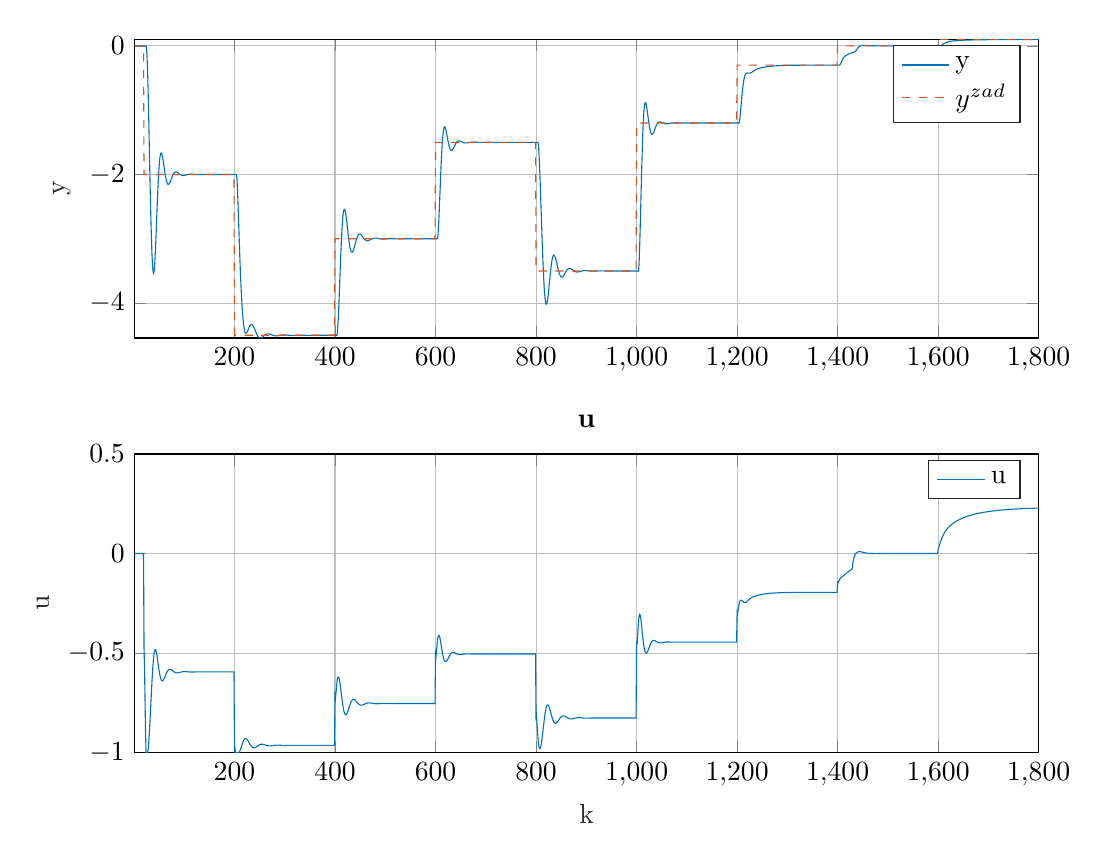
\begin{tikzpicture}

\begin{axis}[%
width=4.521in,
height=1.493in,
at={(0.758in,2.554in)},
scale only axis,
xmin=1,
xmax=1800,
ymin=-4.5419,
ymax=0.1,
ylabel style={font=\color{white!15!black}},
ylabel={y},
axis background/.style={fill=white},
xmajorgrids,
ymajorgrids,
legend style={legend cell align=left, align=left, draw=white!15!black}
]
\addplot [color=mycolor1]
  table[row sep=crcr]{%
1	0\\
2	0\\
3	0\\
4	0\\
5	0\\
6	0\\
7	0\\
8	0\\
9	0\\
10	0\\
11	0\\
12	0\\
13	0\\
14	0\\
15	0\\
16	0\\
17	0\\
18	0\\
19	0\\
20	0\\
21	0\\
22	0\\
23	0\\
24	0\\
25	-0.046722\\
26	-0.17222\\
27	-0.37125\\
28	-0.64589\\
29	-0.98751\\
30	-1.3671\\
31	-1.7547\\
32	-2.1308\\
33	-2.4813\\
34	-2.7944\\
35	-3.06\\
36	-3.2706\\
37	-3.4213\\
38	-3.5099\\
39	-3.5368\\
40	-3.5049\\
41	-3.4197\\
42	-3.2891\\
43	-3.123\\
44	-2.9326\\
45	-2.7299\\
46	-2.5263\\
47	-2.3322\\
48	-2.1559\\
49	-2.0037\\
50	-1.8791\\
51	-1.7839\\
52	-1.7177\\
53	-1.6789\\
54	-1.6647\\
55	-1.6716\\
56	-1.6959\\
57	-1.7335\\
58	-1.7806\\
59	-1.8334\\
60	-1.8884\\
61	-1.9427\\
62	-1.9938\\
63	-2.0396\\
64	-2.0787\\
65	-2.1099\\
66	-2.1328\\
67	-2.1474\\
68	-2.154\\
69	-2.1533\\
70	-2.1462\\
71	-2.1338\\
72	-2.1174\\
73	-2.0983\\
74	-2.0777\\
75	-2.0567\\
76	-2.0364\\
77	-2.0176\\
78	-2.0009\\
79	-1.9869\\
80	-1.9757\\
81	-1.9675\\
82	-1.9622\\
83	-1.9597\\
84	-1.9596\\
85	-1.9616\\
86	-1.9653\\
87	-1.9702\\
88	-1.9759\\
89	-1.9821\\
90	-1.9884\\
91	-1.9944\\
92	-1.9999\\
93	-2.0048\\
94	-2.0088\\
95	-2.0118\\
96	-2.014\\
97	-2.0152\\
98	-2.0156\\
99	-2.0152\\
100	-2.0142\\
101	-2.0127\\
102	-2.0109\\
103	-2.0088\\
104	-2.0066\\
105	-2.0044\\
106	-2.0024\\
107	-2.0005\\
108	-1.9989\\
109	-1.9976\\
110	-1.9966\\
111	-1.9959\\
112	-1.9955\\
113	-1.9954\\
114	-1.9955\\
115	-1.9959\\
116	-1.9963\\
117	-1.9969\\
118	-1.9976\\
119	-1.9983\\
120	-1.999\\
121	-1.9996\\
122	-2.0002\\
123	-2.0007\\
124	-2.001\\
125	-2.0013\\
126	-2.0015\\
127	-2.0016\\
128	-2.0016\\
129	-2.0015\\
130	-2.0014\\
131	-2.0012\\
132	-2.001\\
133	-2.0008\\
134	-2.0006\\
135	-2.0003\\
136	-2.0001\\
137	-1.9999\\
138	-1.9998\\
139	-1.9997\\
140	-1.9996\\
141	-1.9995\\
142	-1.9995\\
143	-1.9995\\
144	-1.9995\\
145	-1.9996\\
146	-1.9996\\
147	-1.9997\\
148	-1.9998\\
149	-1.9998\\
150	-1.9999\\
151	-2\\
152	-2\\
153	-2.0001\\
154	-2.0001\\
155	-2.0002\\
156	-2.0002\\
157	-2.0002\\
158	-2.0002\\
159	-2.0002\\
160	-2.0001\\
161	-2.0001\\
162	-2.0001\\
163	-2.0001\\
164	-2\\
165	-2\\
166	-2\\
167	-2\\
168	-2\\
169	-2\\
170	-2\\
171	-1.9999\\
172	-1.9999\\
173	-1.9999\\
174	-2\\
175	-2\\
176	-2\\
177	-2\\
178	-2\\
179	-2\\
180	-2\\
181	-2\\
182	-2\\
183	-2\\
184	-2\\
185	-2\\
186	-2\\
187	-2\\
188	-2\\
189	-2\\
190	-2\\
191	-2\\
192	-2\\
193	-2\\
194	-2\\
195	-2\\
196	-2\\
197	-2\\
198	-2\\
199	-2\\
200	-2\\
201	-2\\
202	-2\\
203	-2\\
204	-2\\
205	-2.0801\\
206	-2.2427\\
207	-2.4526\\
208	-2.6856\\
209	-2.9234\\
210	-3.1541\\
211	-3.3704\\
212	-3.5682\\
213	-3.7459\\
214	-3.903\\
215	-4.0393\\
216	-4.155\\
217	-4.2505\\
218	-4.3267\\
219	-4.3847\\
220	-4.426\\
221	-4.4525\\
222	-4.4661\\
223	-4.4689\\
224	-4.4632\\
225	-4.451\\
226	-4.4346\\
227	-4.4158\\
228	-4.3963\\
229	-4.3778\\
230	-4.3614\\
231	-4.3482\\
232	-4.3387\\
233	-4.3334\\
234	-4.3325\\
235	-4.3358\\
236	-4.3431\\
237	-4.354\\
238	-4.3678\\
239	-4.3839\\
240	-4.4017\\
241	-4.4205\\
242	-4.4394\\
243	-4.458\\
244	-4.4756\\
245	-4.4917\\
246	-4.5059\\
247	-4.5179\\
248	-4.5275\\
249	-4.5347\\
250	-4.5394\\
251	-4.5418\\
252	-4.5419\\
253	-4.5402\\
254	-4.5368\\
255	-4.532\\
256	-4.5263\\
257	-4.52\\
258	-4.5133\\
259	-4.5066\\
260	-4.5002\\
261	-4.4944\\
262	-4.4892\\
263	-4.4849\\
264	-4.4816\\
265	-4.4792\\
266	-4.4779\\
267	-4.4775\\
268	-4.478\\
269	-4.4793\\
270	-4.4812\\
271	-4.4836\\
272	-4.4865\\
273	-4.4895\\
274	-4.4927\\
275	-4.4958\\
276	-4.4988\\
277	-4.5015\\
278	-4.5038\\
279	-4.5058\\
280	-4.5073\\
281	-4.5084\\
282	-4.5091\\
283	-4.5093\\
284	-4.5091\\
285	-4.5086\\
286	-4.5078\\
287	-4.5067\\
288	-4.5055\\
289	-4.5042\\
290	-4.5028\\
291	-4.5015\\
292	-4.5002\\
293	-4.4991\\
294	-4.4981\\
295	-4.4973\\
296	-4.4966\\
297	-4.4962\\
298	-4.4959\\
299	-4.4958\\
300	-4.496\\
301	-4.4962\\
302	-4.4966\\
303	-4.4971\\
304	-4.4976\\
305	-4.4982\\
306	-4.4988\\
307	-4.4994\\
308	-4.4999\\
309	-4.5004\\
310	-4.5009\\
311	-4.5012\\
312	-4.5015\\
313	-4.5017\\
314	-4.5018\\
315	-4.5018\\
316	-4.5018\\
317	-4.5016\\
318	-4.5015\\
319	-4.5013\\
320	-4.501\\
321	-4.5008\\
322	-4.5005\\
323	-4.5003\\
324	-4.5\\
325	-4.4998\\
326	-4.4996\\
327	-4.4995\\
328	-4.4993\\
329	-4.4993\\
330	-4.4992\\
331	-4.4992\\
332	-4.4992\\
333	-4.4993\\
334	-4.4994\\
335	-4.4995\\
336	-4.4996\\
337	-4.4997\\
338	-4.4998\\
339	-4.4999\\
340	-4.5\\
341	-4.5001\\
342	-4.5002\\
343	-4.5002\\
344	-4.5003\\
345	-4.5003\\
346	-4.5003\\
347	-4.5003\\
348	-4.5003\\
349	-4.5003\\
350	-4.5003\\
351	-4.5002\\
352	-4.5002\\
353	-4.5001\\
354	-4.5001\\
355	-4.5\\
356	-4.5\\
357	-4.5\\
358	-4.4999\\
359	-4.4999\\
360	-4.4999\\
361	-4.4999\\
362	-4.4998\\
363	-4.4998\\
364	-4.4999\\
365	-4.4999\\
366	-4.4999\\
367	-4.4999\\
368	-4.4999\\
369	-4.4999\\
370	-4.5\\
371	-4.5\\
372	-4.5\\
373	-4.5\\
374	-4.5\\
375	-4.5\\
376	-4.5001\\
377	-4.5001\\
378	-4.5001\\
379	-4.5001\\
380	-4.5001\\
381	-4.5001\\
382	-4.5001\\
383	-4.5\\
384	-4.5\\
385	-4.5\\
386	-4.5\\
387	-4.5\\
388	-4.5\\
389	-4.5\\
390	-4.5\\
391	-4.5\\
392	-4.5\\
393	-4.5\\
394	-4.5\\
395	-4.5\\
396	-4.5\\
397	-4.5\\
398	-4.5\\
399	-4.5\\
400	-4.5\\
401	-4.5\\
402	-4.5\\
403	-4.5\\
404	-4.5\\
405	-4.4319\\
406	-4.3057\\
407	-4.143\\
408	-3.9553\\
409	-3.7516\\
410	-3.5418\\
411	-3.3365\\
412	-3.1448\\
413	-2.9739\\
414	-2.8288\\
415	-2.7127\\
416	-2.6269\\
417	-2.5708\\
418	-2.5429\\
419	-2.5405\\
420	-2.5601\\
421	-2.598\\
422	-2.65\\
423	-2.7121\\
424	-2.7804\\
425	-2.851\\
426	-2.9208\\
427	-2.9868\\
428	-3.0467\\
429	-3.0985\\
430	-3.1409\\
431	-3.1731\\
432	-3.1949\\
433	-3.2063\\
434	-3.2081\\
435	-3.2012\\
436	-3.1867\\
437	-3.1662\\
438	-3.1412\\
439	-3.1133\\
440	-3.0839\\
441	-3.0545\\
442	-3.0265\\
443	-3.0007\\
444	-2.9781\\
445	-2.9593\\
446	-2.9446\\
447	-2.9341\\
448	-2.9279\\
449	-2.9256\\
450	-2.9268\\
451	-2.9311\\
452	-2.938\\
453	-2.9468\\
454	-2.9569\\
455	-2.9677\\
456	-2.9786\\
457	-2.9893\\
458	-2.9992\\
459	-3.008\\
460	-3.0155\\
461	-3.0215\\
462	-3.0258\\
463	-3.0286\\
464	-3.0298\\
465	-3.0297\\
466	-3.0282\\
467	-3.0258\\
468	-3.0225\\
469	-3.0187\\
470	-3.0145\\
471	-3.0102\\
472	-3.0059\\
473	-3.0019\\
474	-2.9983\\
475	-2.9952\\
476	-2.9927\\
477	-2.9908\\
478	-2.9895\\
479	-2.9888\\
480	-2.9887\\
481	-2.9891\\
482	-2.9899\\
483	-2.9911\\
484	-2.9925\\
485	-2.994\\
486	-2.9957\\
487	-2.9973\\
488	-2.9989\\
489	-3.0003\\
490	-3.0016\\
491	-3.0026\\
492	-3.0034\\
493	-3.004\\
494	-3.0043\\
495	-3.0044\\
496	-3.0043\\
497	-3.004\\
498	-3.0036\\
499	-3.0031\\
500	-3.0025\\
501	-3.0019\\
502	-3.0012\\
503	-3.0006\\
504	-3.0001\\
505	-2.9996\\
506	-2.9991\\
507	-2.9988\\
508	-2.9985\\
509	-2.9984\\
510	-2.9983\\
511	-2.9983\\
512	-2.9984\\
513	-2.9986\\
514	-2.9987\\
515	-2.999\\
516	-2.9992\\
517	-2.9994\\
518	-2.9997\\
519	-2.9999\\
520	-3.0001\\
521	-3.0003\\
522	-3.0004\\
523	-3.0005\\
524	-3.0006\\
525	-3.0006\\
526	-3.0007\\
527	-3.0006\\
528	-3.0006\\
529	-3.0005\\
530	-3.0004\\
531	-3.0003\\
532	-3.0002\\
533	-3.0001\\
534	-3.0001\\
535	-3\\
536	-2.9999\\
537	-2.9998\\
538	-2.9998\\
539	-2.9998\\
540	-2.9998\\
541	-2.9997\\
542	-2.9998\\
543	-2.9998\\
544	-2.9998\\
545	-2.9998\\
546	-2.9999\\
547	-2.9999\\
548	-2.9999\\
549	-3\\
550	-3\\
551	-3\\
552	-3.0001\\
553	-3.0001\\
554	-3.0001\\
555	-3.0001\\
556	-3.0001\\
557	-3.0001\\
558	-3.0001\\
559	-3.0001\\
560	-3.0001\\
561	-3.0001\\
562	-3\\
563	-3\\
564	-3\\
565	-3\\
566	-3\\
567	-3\\
568	-3\\
569	-3\\
570	-3\\
571	-3\\
572	-3\\
573	-3\\
574	-3\\
575	-3\\
576	-3\\
577	-3\\
578	-3\\
579	-3\\
580	-3\\
581	-3\\
582	-3\\
583	-3\\
584	-3\\
585	-3\\
586	-3\\
587	-3\\
588	-3\\
589	-3\\
590	-3\\
591	-3\\
592	-3\\
593	-3\\
594	-3\\
595	-3\\
596	-3\\
597	-3\\
598	-3\\
599	-3\\
600	-3\\
601	-3\\
602	-3\\
603	-3\\
604	-3\\
605	-2.9262\\
606	-2.7955\\
607	-2.631\\
608	-2.4459\\
609	-2.2501\\
610	-2.0544\\
611	-1.8697\\
612	-1.704\\
613	-1.5627\\
614	-1.4488\\
615	-1.363\\
616	-1.3044\\
617	-1.2709\\
618	-1.2593\\
619	-1.266\\
620	-1.2872\\
621	-1.3192\\
622	-1.3582\\
623	-1.401\\
624	-1.4446\\
625	-1.4866\\
626	-1.5249\\
627	-1.558\\
628	-1.5849\\
629	-1.6051\\
630	-1.6185\\
631	-1.6252\\
632	-1.6259\\
633	-1.6214\\
634	-1.6125\\
635	-1.6003\\
636	-1.5858\\
637	-1.5701\\
638	-1.5541\\
639	-1.5386\\
640	-1.5242\\
641	-1.5115\\
642	-1.5007\\
643	-1.4921\\
644	-1.4858\\
645	-1.4815\\
646	-1.4792\\
647	-1.4787\\
648	-1.4796\\
649	-1.4816\\
650	-1.4845\\
651	-1.488\\
652	-1.4917\\
653	-1.4954\\
654	-1.4989\\
655	-1.502\\
656	-1.5047\\
657	-1.5069\\
658	-1.5084\\
659	-1.5094\\
660	-1.5099\\
661	-1.5098\\
662	-1.5094\\
663	-1.5086\\
664	-1.5076\\
665	-1.5064\\
666	-1.5051\\
667	-1.5039\\
668	-1.5026\\
669	-1.5015\\
670	-1.5005\\
671	-1.4997\\
672	-1.4991\\
673	-1.4986\\
674	-1.4983\\
675	-1.4982\\
676	-1.4982\\
677	-1.4983\\
678	-1.4985\\
679	-1.4987\\
680	-1.499\\
681	-1.4993\\
682	-1.4996\\
683	-1.4999\\
684	-1.5002\\
685	-1.5004\\
686	-1.5006\\
687	-1.5007\\
688	-1.5007\\
689	-1.5008\\
690	-1.5008\\
691	-1.5007\\
692	-1.5007\\
693	-1.5006\\
694	-1.5005\\
695	-1.5004\\
696	-1.5003\\
697	-1.5002\\
698	-1.5001\\
699	-1.5\\
700	-1.5\\
701	-1.4999\\
702	-1.4999\\
703	-1.4999\\
704	-1.4998\\
705	-1.4998\\
706	-1.4999\\
707	-1.4999\\
708	-1.4999\\
709	-1.4999\\
710	-1.4999\\
711	-1.5\\
712	-1.5\\
713	-1.5\\
714	-1.5\\
715	-1.5\\
716	-1.5001\\
717	-1.5001\\
718	-1.5001\\
719	-1.5001\\
720	-1.5001\\
721	-1.5001\\
722	-1.5\\
723	-1.5\\
724	-1.5\\
725	-1.5\\
726	-1.5\\
727	-1.5\\
728	-1.5\\
729	-1.5\\
730	-1.5\\
731	-1.5\\
732	-1.5\\
733	-1.5\\
734	-1.5\\
735	-1.5\\
736	-1.5\\
737	-1.5\\
738	-1.5\\
739	-1.5\\
740	-1.5\\
741	-1.5\\
742	-1.5\\
743	-1.5\\
744	-1.5\\
745	-1.5\\
746	-1.5\\
747	-1.5\\
748	-1.5\\
749	-1.5\\
750	-1.5\\
751	-1.5\\
752	-1.5\\
753	-1.5\\
754	-1.5\\
755	-1.5\\
756	-1.5\\
757	-1.5\\
758	-1.5\\
759	-1.5\\
760	-1.5\\
761	-1.5\\
762	-1.5\\
763	-1.5\\
764	-1.5\\
765	-1.5\\
766	-1.5\\
767	-1.5\\
768	-1.5\\
769	-1.5\\
770	-1.5\\
771	-1.5\\
772	-1.5\\
773	-1.5\\
774	-1.5\\
775	-1.5\\
776	-1.5\\
777	-1.5\\
778	-1.5\\
779	-1.5\\
780	-1.5\\
781	-1.5\\
782	-1.5\\
783	-1.5\\
784	-1.5\\
785	-1.5\\
786	-1.5\\
787	-1.5\\
788	-1.5\\
789	-1.5\\
790	-1.5\\
791	-1.5\\
792	-1.5\\
793	-1.5\\
794	-1.5\\
795	-1.5\\
796	-1.5\\
797	-1.5\\
798	-1.5\\
799	-1.5\\
800	-1.5\\
801	-1.5\\
802	-1.5\\
803	-1.5\\
804	-1.5\\
805	-1.567\\
806	-1.7013\\
807	-1.877\\
808	-2.0809\\
809	-2.3039\\
810	-2.5375\\
811	-2.7728\\
812	-3.0019\\
813	-3.2178\\
814	-3.4145\\
815	-3.5876\\
816	-3.7335\\
817	-3.8499\\
818	-3.9358\\
819	-3.9911\\
820	-4.0172\\
821	-4.0161\\
822	-3.9909\\
823	-3.9454\\
824	-3.8839\\
825	-3.8108\\
826	-3.7307\\
827	-3.6481\\
828	-3.5669\\
829	-3.4908\\
830	-3.4227\\
831	-3.3645\\
832	-3.3179\\
833	-3.2836\\
834	-3.2617\\
835	-3.2518\\
836	-3.2529\\
837	-3.2638\\
838	-3.283\\
839	-3.3087\\
840	-3.3393\\
841	-3.3729\\
842	-3.4078\\
843	-3.4426\\
844	-3.4758\\
845	-3.5062\\
846	-3.533\\
847	-3.5554\\
848	-3.573\\
849	-3.5856\\
850	-3.5932\\
851	-3.596\\
852	-3.5945\\
853	-3.5892\\
854	-3.5807\\
855	-3.5697\\
856	-3.5569\\
857	-3.5432\\
858	-3.5291\\
859	-3.5153\\
860	-3.5024\\
861	-3.4908\\
862	-3.4808\\
863	-3.4727\\
864	-3.4666\\
865	-3.4626\\
866	-3.4605\\
867	-3.4604\\
868	-3.4619\\
869	-3.4648\\
870	-3.4688\\
871	-3.4737\\
872	-3.4792\\
873	-3.4849\\
874	-3.4906\\
875	-3.4961\\
876	-3.5011\\
877	-3.5056\\
878	-3.5093\\
879	-3.5122\\
880	-3.5143\\
881	-3.5156\\
882	-3.5161\\
883	-3.5159\\
884	-3.515\\
885	-3.5136\\
886	-3.5118\\
887	-3.5096\\
888	-3.5074\\
889	-3.505\\
890	-3.5027\\
891	-3.5006\\
892	-3.4986\\
893	-3.497\\
894	-3.4956\\
895	-3.4946\\
896	-3.4939\\
897	-3.4935\\
898	-3.4935\\
899	-3.4937\\
900	-3.4941\\
901	-3.4948\\
902	-3.4956\\
903	-3.4965\\
904	-3.4974\\
905	-3.4984\\
906	-3.4993\\
907	-3.5001\\
908	-3.5009\\
909	-3.5015\\
910	-3.502\\
911	-3.5024\\
912	-3.5026\\
913	-3.5027\\
914	-3.5026\\
915	-3.5025\\
916	-3.5023\\
917	-3.502\\
918	-3.5016\\
919	-3.5012\\
920	-3.5009\\
921	-3.5005\\
922	-3.5001\\
923	-3.4998\\
924	-3.4995\\
925	-3.4993\\
926	-3.4991\\
927	-3.499\\
928	-3.4989\\
929	-3.4989\\
930	-3.4989\\
931	-3.499\\
932	-3.4991\\
933	-3.4993\\
934	-3.4994\\
935	-3.4996\\
936	-3.4997\\
937	-3.4999\\
938	-3.5\\
939	-3.5001\\
940	-3.5002\\
941	-3.5003\\
942	-3.5004\\
943	-3.5004\\
944	-3.5004\\
945	-3.5004\\
946	-3.5004\\
947	-3.5004\\
948	-3.5003\\
949	-3.5003\\
950	-3.5002\\
951	-3.5001\\
952	-3.5001\\
953	-3.5\\
954	-3.5\\
955	-3.4999\\
956	-3.4999\\
957	-3.4999\\
958	-3.4998\\
959	-3.4998\\
960	-3.4998\\
961	-3.4998\\
962	-3.4998\\
963	-3.4999\\
964	-3.4999\\
965	-3.4999\\
966	-3.4999\\
967	-3.5\\
968	-3.5\\
969	-3.5\\
970	-3.5\\
971	-3.5\\
972	-3.5001\\
973	-3.5001\\
974	-3.5001\\
975	-3.5001\\
976	-3.5001\\
977	-3.5001\\
978	-3.5001\\
979	-3.5001\\
980	-3.5\\
981	-3.5\\
982	-3.5\\
983	-3.5\\
984	-3.5\\
985	-3.5\\
986	-3.5\\
987	-3.5\\
988	-3.5\\
989	-3.5\\
990	-3.5\\
991	-3.5\\
992	-3.5\\
993	-3.5\\
994	-3.5\\
995	-3.5\\
996	-3.5\\
997	-3.5\\
998	-3.5\\
999	-3.5\\
1000	-3.5\\
1001	-3.5\\
1002	-3.5\\
1003	-3.5\\
1004	-3.5\\
1005	-3.3746\\
1006	-3.1592\\
1007	-2.8907\\
1008	-2.5911\\
1009	-2.2772\\
1010	-1.9699\\
1011	-1.6876\\
1012	-1.4432\\
1013	-1.2434\\
1014	-1.0904\\
1015	-0.98243\\
1016	-0.91576\\
1017	-0.88498\\
1018	-0.88403\\
1019	-0.90662\\
1020	-0.94665\\
1021	-0.9984\\
1022	-1.0567\\
1023	-1.1171\\
1024	-1.1757\\
1025	-1.2296\\
1026	-1.2766\\
1027	-1.315\\
1028	-1.344\\
1029	-1.3635\\
1030	-1.3737\\
1031	-1.3755\\
1032	-1.3699\\
1033	-1.3582\\
1034	-1.3421\\
1035	-1.3229\\
1036	-1.3021\\
1037	-1.2809\\
1038	-1.2605\\
1039	-1.2416\\
1040	-1.225\\
1041	-1.211\\
1042	-1.1999\\
1043	-1.1916\\
1044	-1.1861\\
1045	-1.183\\
1046	-1.182\\
1047	-1.1828\\
1048	-1.1849\\
1049	-1.1879\\
1050	-1.1915\\
1051	-1.1954\\
1052	-1.1992\\
1053	-1.2028\\
1054	-1.2059\\
1055	-1.2084\\
1056	-1.2103\\
1057	-1.2116\\
1058	-1.2123\\
1059	-1.2124\\
1060	-1.212\\
1061	-1.2112\\
1062	-1.2102\\
1063	-1.2089\\
1064	-1.2075\\
1065	-1.2061\\
1066	-1.2047\\
1067	-1.2035\\
1068	-1.2023\\
1069	-1.2014\\
1070	-1.2006\\
1071	-1.2\\
1072	-1.1996\\
1073	-1.1993\\
1074	-1.1992\\
1075	-1.1992\\
1076	-1.1993\\
1077	-1.1994\\
1078	-1.1996\\
1079	-1.1999\\
1080	-1.2001\\
1081	-1.2003\\
1082	-1.2005\\
1083	-1.2006\\
1084	-1.2008\\
1085	-1.2008\\
1086	-1.2009\\
1087	-1.2009\\
1088	-1.2009\\
1089	-1.2008\\
1090	-1.2007\\
1091	-1.2007\\
1092	-1.2006\\
1093	-1.2005\\
1094	-1.2004\\
1095	-1.2003\\
1096	-1.2002\\
1097	-1.2001\\
1098	-1.2001\\
1099	-1.2\\
1100	-1.2\\
1101	-1.2\\
1102	-1.2\\
1103	-1.2\\
1104	-1.2\\
1105	-1.2\\
1106	-1.2\\
1107	-1.2\\
1108	-1.2\\
1109	-1.2\\
1110	-1.2\\
1111	-1.2001\\
1112	-1.2001\\
1113	-1.2001\\
1114	-1.2001\\
1115	-1.2001\\
1116	-1.2001\\
1117	-1.2001\\
1118	-1.2001\\
1119	-1.2\\
1120	-1.2\\
1121	-1.2\\
1122	-1.2\\
1123	-1.2\\
1124	-1.2\\
1125	-1.2\\
1126	-1.2\\
1127	-1.2\\
1128	-1.2\\
1129	-1.2\\
1130	-1.2\\
1131	-1.2\\
1132	-1.2\\
1133	-1.2\\
1134	-1.2\\
1135	-1.2\\
1136	-1.2\\
1137	-1.2\\
1138	-1.2\\
1139	-1.2\\
1140	-1.2\\
1141	-1.2\\
1142	-1.2\\
1143	-1.2\\
1144	-1.2\\
1145	-1.2\\
1146	-1.2\\
1147	-1.2\\
1148	-1.2\\
1149	-1.2\\
1150	-1.2\\
1151	-1.2\\
1152	-1.2\\
1153	-1.2\\
1154	-1.2\\
1155	-1.2\\
1156	-1.2\\
1157	-1.2\\
1158	-1.2\\
1159	-1.2\\
1160	-1.2\\
1161	-1.2\\
1162	-1.2\\
1163	-1.2\\
1164	-1.2\\
1165	-1.2\\
1166	-1.2\\
1167	-1.2\\
1168	-1.2\\
1169	-1.2\\
1170	-1.2\\
1171	-1.2\\
1172	-1.2\\
1173	-1.2\\
1174	-1.2\\
1175	-1.2\\
1176	-1.2\\
1177	-1.2\\
1178	-1.2\\
1179	-1.2\\
1180	-1.2\\
1181	-1.2\\
1182	-1.2\\
1183	-1.2\\
1184	-1.2\\
1185	-1.2\\
1186	-1.2\\
1187	-1.2\\
1188	-1.2\\
1189	-1.2\\
1190	-1.2\\
1191	-1.2\\
1192	-1.2\\
1193	-1.2\\
1194	-1.2\\
1195	-1.2\\
1196	-1.2\\
1197	-1.2\\
1198	-1.2\\
1199	-1.2\\
1200	-1.2\\
1201	-1.2\\
1202	-1.2\\
1203	-1.2\\
1204	-1.2\\
1205	-1.1595\\
1206	-1.0904\\
1207	-1.0075\\
1208	-0.91874\\
1209	-0.82958\\
1210	-0.7449\\
1211	-0.66863\\
1212	-0.60311\\
1213	-0.54926\\
1214	-0.50692\\
1215	-0.4752\\
1216	-0.45274\\
1217	-0.43794\\
1218	-0.42911\\
1219	-0.42465\\
1220	-0.42312\\
1221	-0.42329\\
1222	-0.42418\\
1223	-0.42504\\
1224	-0.42536\\
1225	-0.42481\\
1226	-0.42326\\
1227	-0.4207\\
1228	-0.41721\\
1229	-0.41295\\
1230	-0.40811\\
1231	-0.40289\\
1232	-0.39746\\
1233	-0.392\\
1234	-0.38665\\
1235	-0.38152\\
1236	-0.37667\\
1237	-0.37216\\
1238	-0.36799\\
1239	-0.36418\\
1240	-0.3607\\
1241	-0.35754\\
1242	-0.35465\\
1243	-0.352\\
1244	-0.34956\\
1245	-0.34729\\
1246	-0.34517\\
1247	-0.34318\\
1248	-0.34129\\
1249	-0.33949\\
1250	-0.33777\\
1251	-0.33611\\
1252	-0.33452\\
1253	-0.33299\\
1254	-0.33152\\
1255	-0.33011\\
1256	-0.32875\\
1257	-0.32745\\
1258	-0.3262\\
1259	-0.32501\\
1260	-0.32388\\
1261	-0.32279\\
1262	-0.32176\\
1263	-0.32077\\
1264	-0.31984\\
1265	-0.31895\\
1266	-0.3181\\
1267	-0.31729\\
1268	-0.31651\\
1269	-0.31578\\
1270	-0.31508\\
1271	-0.31441\\
1272	-0.31377\\
1273	-0.31316\\
1274	-0.31258\\
1275	-0.31203\\
1276	-0.3115\\
1277	-0.31099\\
1278	-0.31051\\
1279	-0.31005\\
1280	-0.3096\\
1281	-0.30918\\
1282	-0.30878\\
1283	-0.30839\\
1284	-0.30802\\
1285	-0.30767\\
1286	-0.30733\\
1287	-0.30701\\
1288	-0.30671\\
1289	-0.30641\\
1290	-0.30613\\
1291	-0.30586\\
1292	-0.30561\\
1293	-0.30536\\
1294	-0.30513\\
1295	-0.3049\\
1296	-0.30469\\
1297	-0.30448\\
1298	-0.30429\\
1299	-0.3041\\
1300	-0.30392\\
1301	-0.30375\\
1302	-0.30359\\
1303	-0.30343\\
1304	-0.30328\\
1305	-0.30314\\
1306	-0.303\\
1307	-0.30287\\
1308	-0.30275\\
1309	-0.30263\\
1310	-0.30251\\
1311	-0.3024\\
1312	-0.3023\\
1313	-0.3022\\
1314	-0.3021\\
1315	-0.30201\\
1316	-0.30192\\
1317	-0.30184\\
1318	-0.30176\\
1319	-0.30168\\
1320	-0.30161\\
1321	-0.30154\\
1322	-0.30147\\
1323	-0.30141\\
1324	-0.30135\\
1325	-0.30129\\
1326	-0.30123\\
1327	-0.30118\\
1328	-0.30113\\
1329	-0.30108\\
1330	-0.30103\\
1331	-0.30099\\
1332	-0.30095\\
1333	-0.3009\\
1334	-0.30087\\
1335	-0.30083\\
1336	-0.30079\\
1337	-0.30076\\
1338	-0.30072\\
1339	-0.30069\\
1340	-0.30066\\
1341	-0.30063\\
1342	-0.30061\\
1343	-0.30058\\
1344	-0.30056\\
1345	-0.30053\\
1346	-0.30051\\
1347	-0.30049\\
1348	-0.30046\\
1349	-0.30044\\
1350	-0.30043\\
1351	-0.30041\\
1352	-0.30039\\
1353	-0.30037\\
1354	-0.30036\\
1355	-0.30034\\
1356	-0.30033\\
1357	-0.30031\\
1358	-0.3003\\
1359	-0.30029\\
1360	-0.30027\\
1361	-0.30026\\
1362	-0.30025\\
1363	-0.30024\\
1364	-0.30023\\
1365	-0.30022\\
1366	-0.30021\\
1367	-0.3002\\
1368	-0.30019\\
1369	-0.30018\\
1370	-0.30018\\
1371	-0.30017\\
1372	-0.30016\\
1373	-0.30015\\
1374	-0.30015\\
1375	-0.30014\\
1376	-0.30013\\
1377	-0.30013\\
1378	-0.30012\\
1379	-0.30012\\
1380	-0.30011\\
1381	-0.30011\\
1382	-0.3001\\
1383	-0.3001\\
1384	-0.30009\\
1385	-0.30009\\
1386	-0.30009\\
1387	-0.30008\\
1388	-0.30008\\
1389	-0.30008\\
1390	-0.30007\\
1391	-0.30007\\
1392	-0.30007\\
1393	-0.30006\\
1394	-0.30006\\
1395	-0.30006\\
1396	-0.30006\\
1397	-0.30005\\
1398	-0.30005\\
1399	-0.30005\\
1400	-0.30005\\
1401	-0.30004\\
1402	-0.30004\\
1403	-0.30004\\
1404	-0.30004\\
1405	-0.2917\\
1406	-0.27707\\
1407	-0.26021\\
1408	-0.24291\\
1409	-0.22617\\
1410	-0.21067\\
1411	-0.19685\\
1412	-0.18488\\
1413	-0.17473\\
1414	-0.16621\\
1415	-0.1591\\
1416	-0.15313\\
1417	-0.14805\\
1418	-0.14361\\
1419	-0.13964\\
1420	-0.13598\\
1421	-0.13252\\
1422	-0.12917\\
1423	-0.12591\\
1424	-0.12269\\
1425	-0.11951\\
1426	-0.11638\\
1427	-0.1133\\
1428	-0.11027\\
1429	-0.10732\\
1430	-0.10445\\
1431	-0.10166\\
1432	-0.098959\\
1433	-0.096353\\
1434	-0.093839\\
1435	-0.089198\\
1436	-0.081196\\
1437	-0.070678\\
1438	-0.059038\\
1439	-0.047265\\
1440	-0.036174\\
1441	-0.026429\\
1442	-0.018324\\
1443	-0.011847\\
1444	-0.0067464\\
1445	-0.0027384\\
1446	0.00037222\\
1447	0.002737\\
1448	0.0044835\\
1449	0.005722\\
1450	0.0065467\\
1451	0.0070376\\
1452	0.0072624\\
1453	0.0072783\\
1454	0.0071332\\
1455	0.0068672\\
1456	0.0065136\\
1457	0.0060996\\
1458	0.0056476\\
1459	0.0051755\\
1460	0.0046977\\
1461	0.0042254\\
1462	0.0037673\\
1463	0.0033298\\
1464	0.0029175\\
1465	0.0025336\\
1466	0.0021798\\
1467	0.0018571\\
1468	0.0015654\\
1469	0.0013042\\
1470	0.0010722\\
1471	0.00086819\\
1472	0.00069025\\
1473	0.00053654\\
1474	0.00040504\\
1475	0.00029373\\
1476	0.00020057\\
1477	0.00012361\\
1478	6.0962e-05\\
1479	1.0834e-05\\
1480	-2.8433e-05\\
1481	-5.8371e-05\\
1482	-8.0383e-05\\
1483	-9.5734e-05\\
1484	-0.00010556\\
1485	-0.00011086\\
1486	-0.00011252\\
1487	-0.00011131\\
1488	-0.0001079\\
1489	-0.00010284\\
1490	-9.6611e-05\\
1491	-8.9615e-05\\
1492	-8.2175e-05\\
1493	-7.4555e-05\\
1494	-6.6964e-05\\
1495	-5.9564e-05\\
1496	-5.2479e-05\\
1497	-4.5795e-05\\
1498	-3.9574e-05\\
1499	-3.3849e-05\\
1500	-2.864e-05\\
1501	-2.3948e-05\\
1502	-1.9762e-05\\
1503	-1.6064e-05\\
1504	-1.2827e-05\\
1505	-1.0022e-05\\
1506	-7.6156e-06\\
1507	-5.5726e-06\\
1508	-3.8581e-06\\
1509	-2.4375e-06\\
1510	-1.2773e-06\\
1511	-3.4556e-07\\
1512	3.8752e-07\\
1513	9.4966e-07\\
1514	1.3662e-06\\
1515	1.6602e-06\\
1516	1.8521e-06\\
1517	1.9604e-06\\
1518	2.0012e-06\\
1519	1.9884e-06\\
1520	1.9343e-06\\
1521	1.8492e-06\\
1522	1.7418e-06\\
1523	1.6195e-06\\
1524	1.4882e-06\\
1525	1.353e-06\\
1526	1.2176e-06\\
1527	1.0852e-06\\
1528	9.5793e-07\\
1529	8.3757e-07\\
1530	7.2525e-07\\
1531	6.2168e-07\\
1532	5.2723e-07\\
1533	4.4197e-07\\
1534	3.6577e-07\\
1535	2.9831e-07\\
1536	2.3916e-07\\
1537	1.8779e-07\\
1538	1.4363e-07\\
1539	1.0605e-07\\
1540	7.443e-08\\
1541	4.8162e-08\\
1542	2.6639e-08\\
1543	9.2902e-09\\
1544	-4.4235e-09\\
1545	-1.5002e-08\\
1546	-2.2905e-08\\
1547	-2.8549e-08\\
1548	-3.2309e-08\\
1549	-3.4518e-08\\
1550	-3.547e-08\\
1551	-3.5424e-08\\
1552	-3.46e-08\\
1553	-3.319e-08\\
1554	-3.1354e-08\\
1555	-2.9228e-08\\
1556	-2.6923e-08\\
1557	-2.453e-08\\
1558	-2.2122e-08\\
1559	-1.9755e-08\\
1560	-1.7474e-08\\
1561	-1.5309e-08\\
1562	-1.3283e-08\\
1563	-1.1411e-08\\
1564	-9.6994e-09\\
1565	-8.1514e-09\\
1566	-6.765e-09\\
1567	-5.5352e-09\\
1568	-4.4547e-09\\
1569	-3.5145e-09\\
1570	-2.7043e-09\\
1571	-2.0135e-09\\
1572	-1.4308e-09\\
1573	-9.4541e-10\\
1574	-5.4646e-10\\
1575	-2.237e-10\\
1576	3.2554e-11\\
1577	2.3135e-10\\
1578	3.8098e-10\\
1579	4.8901e-10\\
1580	5.6225e-10\\
1581	6.0677e-10\\
1582	6.2795e-10\\
1583	6.3049e-10\\
1584	6.1845e-10\\
1585	5.9533e-10\\
1586	5.641e-10\\
1587	5.2724e-10\\
1588	4.8683e-10\\
1589	4.4455e-10\\
1590	4.0175e-10\\
1591	3.5949e-10\\
1592	3.1861e-10\\
1593	2.7969e-10\\
1594	2.4318e-10\\
1595	2.0935e-10\\
1596	1.7835e-10\\
1597	1.5026e-10\\
1598	1.2504e-10\\
1599	1.0263e-10\\
1600	8.2904e-11\\
1601	6.5702e-11\\
1602	5.0848e-11\\
1603	3.8153e-11\\
1604	2.7421e-11\\
1605	0.0014818\\
1606	0.0049077\\
1607	0.00936\\
1608	0.014417\\
1609	0.019762\\
1610	0.025159\\
1611	0.030424\\
1612	0.035423\\
1613	0.040075\\
1614	0.044339\\
1615	0.048206\\
1616	0.051687\\
1617	0.054804\\
1618	0.05759\\
1619	0.060079\\
1620	0.062306\\
1621	0.064303\\
1622	0.0661\\
1623	0.067725\\
1624	0.069201\\
1625	0.070547\\
1626	0.071782\\
1627	0.07292\\
1628	0.073972\\
1629	0.07495\\
1630	0.075862\\
1631	0.076716\\
1632	0.077517\\
1633	0.07827\\
1634	0.078982\\
1635	0.079655\\
1636	0.080292\\
1637	0.080897\\
1638	0.081472\\
1639	0.08202\\
1640	0.082543\\
1641	0.083042\\
1642	0.083519\\
1643	0.083976\\
1644	0.084413\\
1645	0.084833\\
1646	0.085235\\
1647	0.085622\\
1648	0.085994\\
1649	0.086352\\
1650	0.086696\\
1651	0.087028\\
1652	0.087348\\
1653	0.087657\\
1654	0.087955\\
1655	0.088243\\
1656	0.088522\\
1657	0.088791\\
1658	0.089051\\
1659	0.089303\\
1660	0.089547\\
1661	0.089783\\
1662	0.090012\\
1663	0.090235\\
1664	0.09045\\
1665	0.090659\\
1666	0.090862\\
1667	0.091059\\
1668	0.091251\\
1669	0.091437\\
1670	0.091618\\
1671	0.091793\\
1672	0.091964\\
1673	0.092131\\
1674	0.092293\\
1675	0.09245\\
1676	0.092604\\
1677	0.092753\\
1678	0.092899\\
1679	0.093041\\
1680	0.093179\\
1681	0.093314\\
1682	0.093446\\
1683	0.093574\\
1684	0.093699\\
1685	0.093821\\
1686	0.09394\\
1687	0.094057\\
1688	0.09417\\
1689	0.094281\\
1690	0.094389\\
1691	0.094495\\
1692	0.094599\\
1693	0.0947\\
1694	0.094798\\
1695	0.094895\\
1696	0.094989\\
1697	0.095081\\
1698	0.095172\\
1699	0.09526\\
1700	0.095346\\
1701	0.095431\\
1702	0.095513\\
1703	0.095594\\
1704	0.095673\\
1705	0.095751\\
1706	0.095827\\
1707	0.095901\\
1708	0.095974\\
1709	0.096045\\
1710	0.096115\\
1711	0.096183\\
1712	0.09625\\
1713	0.096315\\
1714	0.09638\\
1715	0.096443\\
1716	0.096504\\
1717	0.096565\\
1718	0.096624\\
1719	0.096682\\
1720	0.096739\\
1721	0.096795\\
1722	0.09685\\
1723	0.096903\\
1724	0.096956\\
1725	0.097008\\
1726	0.097058\\
1727	0.097108\\
1728	0.097157\\
1729	0.097205\\
1730	0.097252\\
1731	0.097298\\
1732	0.097343\\
1733	0.097387\\
1734	0.097431\\
1735	0.097474\\
1736	0.097515\\
1737	0.097557\\
1738	0.097597\\
1739	0.097637\\
1740	0.097676\\
1741	0.097714\\
1742	0.097751\\
1743	0.097788\\
1744	0.097825\\
1745	0.09786\\
1746	0.097895\\
1747	0.097929\\
1748	0.097963\\
1749	0.097996\\
1750	0.098029\\
1751	0.098061\\
1752	0.098092\\
1753	0.098123\\
1754	0.098153\\
1755	0.098183\\
1756	0.098212\\
1757	0.098241\\
1758	0.098269\\
1759	0.098297\\
1760	0.098324\\
1761	0.098351\\
1762	0.098377\\
1763	0.098403\\
1764	0.098429\\
1765	0.098454\\
1766	0.098478\\
1767	0.098502\\
1768	0.098526\\
1769	0.09855\\
1770	0.098573\\
1771	0.098595\\
1772	0.098617\\
1773	0.098639\\
1774	0.098661\\
1775	0.098682\\
1776	0.098702\\
1777	0.098723\\
1778	0.098743\\
1779	0.098763\\
1780	0.098782\\
1781	0.098801\\
1782	0.09882\\
1783	0.098838\\
1784	0.098857\\
1785	0.098874\\
1786	0.098892\\
1787	0.098909\\
1788	0.098926\\
1789	0.098943\\
1790	0.098959\\
1791	0.098976\\
1792	0.098991\\
1793	0.099007\\
1794	0.099023\\
1795	0.099038\\
1796	0.099053\\
1797	0.099067\\
1798	0.099082\\
1799	0.099096\\
1800	0.09911\\
};
\addlegendentry{y}

\addplot [color=mycolor2, dashed]
  table[row sep=crcr]{%
1	0\\
2	0\\
3	0\\
4	0\\
5	0\\
6	0\\
7	0\\
8	0\\
9	0\\
10	0\\
11	0\\
12	0\\
13	0\\
14	0\\
15	0\\
16	0\\
17	0\\
18	0\\
19	0\\
20	-2\\
21	-2\\
22	-2\\
23	-2\\
24	-2\\
25	-2\\
26	-2\\
27	-2\\
28	-2\\
29	-2\\
30	-2\\
31	-2\\
32	-2\\
33	-2\\
34	-2\\
35	-2\\
36	-2\\
37	-2\\
38	-2\\
39	-2\\
40	-2\\
41	-2\\
42	-2\\
43	-2\\
44	-2\\
45	-2\\
46	-2\\
47	-2\\
48	-2\\
49	-2\\
50	-2\\
51	-2\\
52	-2\\
53	-2\\
54	-2\\
55	-2\\
56	-2\\
57	-2\\
58	-2\\
59	-2\\
60	-2\\
61	-2\\
62	-2\\
63	-2\\
64	-2\\
65	-2\\
66	-2\\
67	-2\\
68	-2\\
69	-2\\
70	-2\\
71	-2\\
72	-2\\
73	-2\\
74	-2\\
75	-2\\
76	-2\\
77	-2\\
78	-2\\
79	-2\\
80	-2\\
81	-2\\
82	-2\\
83	-2\\
84	-2\\
85	-2\\
86	-2\\
87	-2\\
88	-2\\
89	-2\\
90	-2\\
91	-2\\
92	-2\\
93	-2\\
94	-2\\
95	-2\\
96	-2\\
97	-2\\
98	-2\\
99	-2\\
100	-2\\
101	-2\\
102	-2\\
103	-2\\
104	-2\\
105	-2\\
106	-2\\
107	-2\\
108	-2\\
109	-2\\
110	-2\\
111	-2\\
112	-2\\
113	-2\\
114	-2\\
115	-2\\
116	-2\\
117	-2\\
118	-2\\
119	-2\\
120	-2\\
121	-2\\
122	-2\\
123	-2\\
124	-2\\
125	-2\\
126	-2\\
127	-2\\
128	-2\\
129	-2\\
130	-2\\
131	-2\\
132	-2\\
133	-2\\
134	-2\\
135	-2\\
136	-2\\
137	-2\\
138	-2\\
139	-2\\
140	-2\\
141	-2\\
142	-2\\
143	-2\\
144	-2\\
145	-2\\
146	-2\\
147	-2\\
148	-2\\
149	-2\\
150	-2\\
151	-2\\
152	-2\\
153	-2\\
154	-2\\
155	-2\\
156	-2\\
157	-2\\
158	-2\\
159	-2\\
160	-2\\
161	-2\\
162	-2\\
163	-2\\
164	-2\\
165	-2\\
166	-2\\
167	-2\\
168	-2\\
169	-2\\
170	-2\\
171	-2\\
172	-2\\
173	-2\\
174	-2\\
175	-2\\
176	-2\\
177	-2\\
178	-2\\
179	-2\\
180	-2\\
181	-2\\
182	-2\\
183	-2\\
184	-2\\
185	-2\\
186	-2\\
187	-2\\
188	-2\\
189	-2\\
190	-2\\
191	-2\\
192	-2\\
193	-2\\
194	-2\\
195	-2\\
196	-2\\
197	-2\\
198	-2\\
199	-2\\
200	-4.5\\
201	-4.5\\
202	-4.5\\
203	-4.5\\
204	-4.5\\
205	-4.5\\
206	-4.5\\
207	-4.5\\
208	-4.5\\
209	-4.5\\
210	-4.5\\
211	-4.5\\
212	-4.5\\
213	-4.5\\
214	-4.5\\
215	-4.5\\
216	-4.5\\
217	-4.5\\
218	-4.5\\
219	-4.5\\
220	-4.5\\
221	-4.5\\
222	-4.5\\
223	-4.5\\
224	-4.5\\
225	-4.5\\
226	-4.5\\
227	-4.5\\
228	-4.5\\
229	-4.5\\
230	-4.5\\
231	-4.5\\
232	-4.5\\
233	-4.5\\
234	-4.5\\
235	-4.5\\
236	-4.5\\
237	-4.5\\
238	-4.5\\
239	-4.5\\
240	-4.5\\
241	-4.5\\
242	-4.5\\
243	-4.5\\
244	-4.5\\
245	-4.5\\
246	-4.5\\
247	-4.5\\
248	-4.5\\
249	-4.5\\
250	-4.5\\
251	-4.5\\
252	-4.5\\
253	-4.5\\
254	-4.5\\
255	-4.5\\
256	-4.5\\
257	-4.5\\
258	-4.5\\
259	-4.5\\
260	-4.5\\
261	-4.5\\
262	-4.5\\
263	-4.5\\
264	-4.5\\
265	-4.5\\
266	-4.5\\
267	-4.5\\
268	-4.5\\
269	-4.5\\
270	-4.5\\
271	-4.5\\
272	-4.5\\
273	-4.5\\
274	-4.5\\
275	-4.5\\
276	-4.5\\
277	-4.5\\
278	-4.5\\
279	-4.5\\
280	-4.5\\
281	-4.5\\
282	-4.5\\
283	-4.5\\
284	-4.5\\
285	-4.5\\
286	-4.5\\
287	-4.5\\
288	-4.5\\
289	-4.5\\
290	-4.5\\
291	-4.5\\
292	-4.5\\
293	-4.5\\
294	-4.5\\
295	-4.5\\
296	-4.5\\
297	-4.5\\
298	-4.5\\
299	-4.5\\
300	-4.5\\
301	-4.5\\
302	-4.5\\
303	-4.5\\
304	-4.5\\
305	-4.5\\
306	-4.5\\
307	-4.5\\
308	-4.5\\
309	-4.5\\
310	-4.5\\
311	-4.5\\
312	-4.5\\
313	-4.5\\
314	-4.5\\
315	-4.5\\
316	-4.5\\
317	-4.5\\
318	-4.5\\
319	-4.5\\
320	-4.5\\
321	-4.5\\
322	-4.5\\
323	-4.5\\
324	-4.5\\
325	-4.5\\
326	-4.5\\
327	-4.5\\
328	-4.5\\
329	-4.5\\
330	-4.5\\
331	-4.5\\
332	-4.5\\
333	-4.5\\
334	-4.5\\
335	-4.5\\
336	-4.5\\
337	-4.5\\
338	-4.5\\
339	-4.5\\
340	-4.5\\
341	-4.5\\
342	-4.5\\
343	-4.5\\
344	-4.5\\
345	-4.5\\
346	-4.5\\
347	-4.5\\
348	-4.5\\
349	-4.5\\
350	-4.5\\
351	-4.5\\
352	-4.5\\
353	-4.5\\
354	-4.5\\
355	-4.5\\
356	-4.5\\
357	-4.5\\
358	-4.5\\
359	-4.5\\
360	-4.5\\
361	-4.5\\
362	-4.5\\
363	-4.5\\
364	-4.5\\
365	-4.5\\
366	-4.5\\
367	-4.5\\
368	-4.5\\
369	-4.5\\
370	-4.5\\
371	-4.5\\
372	-4.5\\
373	-4.5\\
374	-4.5\\
375	-4.5\\
376	-4.5\\
377	-4.5\\
378	-4.5\\
379	-4.5\\
380	-4.5\\
381	-4.5\\
382	-4.5\\
383	-4.5\\
384	-4.5\\
385	-4.5\\
386	-4.5\\
387	-4.5\\
388	-4.5\\
389	-4.5\\
390	-4.5\\
391	-4.5\\
392	-4.5\\
393	-4.5\\
394	-4.5\\
395	-4.5\\
396	-4.5\\
397	-4.5\\
398	-4.5\\
399	-4.5\\
400	-3\\
401	-3\\
402	-3\\
403	-3\\
404	-3\\
405	-3\\
406	-3\\
407	-3\\
408	-3\\
409	-3\\
410	-3\\
411	-3\\
412	-3\\
413	-3\\
414	-3\\
415	-3\\
416	-3\\
417	-3\\
418	-3\\
419	-3\\
420	-3\\
421	-3\\
422	-3\\
423	-3\\
424	-3\\
425	-3\\
426	-3\\
427	-3\\
428	-3\\
429	-3\\
430	-3\\
431	-3\\
432	-3\\
433	-3\\
434	-3\\
435	-3\\
436	-3\\
437	-3\\
438	-3\\
439	-3\\
440	-3\\
441	-3\\
442	-3\\
443	-3\\
444	-3\\
445	-3\\
446	-3\\
447	-3\\
448	-3\\
449	-3\\
450	-3\\
451	-3\\
452	-3\\
453	-3\\
454	-3\\
455	-3\\
456	-3\\
457	-3\\
458	-3\\
459	-3\\
460	-3\\
461	-3\\
462	-3\\
463	-3\\
464	-3\\
465	-3\\
466	-3\\
467	-3\\
468	-3\\
469	-3\\
470	-3\\
471	-3\\
472	-3\\
473	-3\\
474	-3\\
475	-3\\
476	-3\\
477	-3\\
478	-3\\
479	-3\\
480	-3\\
481	-3\\
482	-3\\
483	-3\\
484	-3\\
485	-3\\
486	-3\\
487	-3\\
488	-3\\
489	-3\\
490	-3\\
491	-3\\
492	-3\\
493	-3\\
494	-3\\
495	-3\\
496	-3\\
497	-3\\
498	-3\\
499	-3\\
500	-3\\
501	-3\\
502	-3\\
503	-3\\
504	-3\\
505	-3\\
506	-3\\
507	-3\\
508	-3\\
509	-3\\
510	-3\\
511	-3\\
512	-3\\
513	-3\\
514	-3\\
515	-3\\
516	-3\\
517	-3\\
518	-3\\
519	-3\\
520	-3\\
521	-3\\
522	-3\\
523	-3\\
524	-3\\
525	-3\\
526	-3\\
527	-3\\
528	-3\\
529	-3\\
530	-3\\
531	-3\\
532	-3\\
533	-3\\
534	-3\\
535	-3\\
536	-3\\
537	-3\\
538	-3\\
539	-3\\
540	-3\\
541	-3\\
542	-3\\
543	-3\\
544	-3\\
545	-3\\
546	-3\\
547	-3\\
548	-3\\
549	-3\\
550	-3\\
551	-3\\
552	-3\\
553	-3\\
554	-3\\
555	-3\\
556	-3\\
557	-3\\
558	-3\\
559	-3\\
560	-3\\
561	-3\\
562	-3\\
563	-3\\
564	-3\\
565	-3\\
566	-3\\
567	-3\\
568	-3\\
569	-3\\
570	-3\\
571	-3\\
572	-3\\
573	-3\\
574	-3\\
575	-3\\
576	-3\\
577	-3\\
578	-3\\
579	-3\\
580	-3\\
581	-3\\
582	-3\\
583	-3\\
584	-3\\
585	-3\\
586	-3\\
587	-3\\
588	-3\\
589	-3\\
590	-3\\
591	-3\\
592	-3\\
593	-3\\
594	-3\\
595	-3\\
596	-3\\
597	-3\\
598	-3\\
599	-3\\
600	-1.5\\
601	-1.5\\
602	-1.5\\
603	-1.5\\
604	-1.5\\
605	-1.5\\
606	-1.5\\
607	-1.5\\
608	-1.5\\
609	-1.5\\
610	-1.5\\
611	-1.5\\
612	-1.5\\
613	-1.5\\
614	-1.5\\
615	-1.5\\
616	-1.5\\
617	-1.5\\
618	-1.5\\
619	-1.5\\
620	-1.5\\
621	-1.5\\
622	-1.5\\
623	-1.5\\
624	-1.5\\
625	-1.5\\
626	-1.5\\
627	-1.5\\
628	-1.5\\
629	-1.5\\
630	-1.5\\
631	-1.5\\
632	-1.5\\
633	-1.5\\
634	-1.5\\
635	-1.5\\
636	-1.5\\
637	-1.5\\
638	-1.5\\
639	-1.5\\
640	-1.5\\
641	-1.5\\
642	-1.5\\
643	-1.5\\
644	-1.5\\
645	-1.5\\
646	-1.5\\
647	-1.5\\
648	-1.5\\
649	-1.5\\
650	-1.5\\
651	-1.5\\
652	-1.5\\
653	-1.5\\
654	-1.5\\
655	-1.5\\
656	-1.5\\
657	-1.5\\
658	-1.5\\
659	-1.5\\
660	-1.5\\
661	-1.5\\
662	-1.5\\
663	-1.5\\
664	-1.5\\
665	-1.5\\
666	-1.5\\
667	-1.5\\
668	-1.5\\
669	-1.5\\
670	-1.5\\
671	-1.5\\
672	-1.5\\
673	-1.5\\
674	-1.5\\
675	-1.5\\
676	-1.5\\
677	-1.5\\
678	-1.5\\
679	-1.5\\
680	-1.5\\
681	-1.5\\
682	-1.5\\
683	-1.5\\
684	-1.5\\
685	-1.5\\
686	-1.5\\
687	-1.5\\
688	-1.5\\
689	-1.5\\
690	-1.5\\
691	-1.5\\
692	-1.5\\
693	-1.5\\
694	-1.5\\
695	-1.5\\
696	-1.5\\
697	-1.5\\
698	-1.5\\
699	-1.5\\
700	-1.5\\
701	-1.5\\
702	-1.5\\
703	-1.5\\
704	-1.5\\
705	-1.5\\
706	-1.5\\
707	-1.5\\
708	-1.5\\
709	-1.5\\
710	-1.5\\
711	-1.5\\
712	-1.5\\
713	-1.5\\
714	-1.5\\
715	-1.5\\
716	-1.5\\
717	-1.5\\
718	-1.5\\
719	-1.5\\
720	-1.5\\
721	-1.5\\
722	-1.5\\
723	-1.5\\
724	-1.5\\
725	-1.5\\
726	-1.5\\
727	-1.5\\
728	-1.5\\
729	-1.5\\
730	-1.5\\
731	-1.5\\
732	-1.5\\
733	-1.5\\
734	-1.5\\
735	-1.5\\
736	-1.5\\
737	-1.5\\
738	-1.5\\
739	-1.5\\
740	-1.5\\
741	-1.5\\
742	-1.5\\
743	-1.5\\
744	-1.5\\
745	-1.5\\
746	-1.5\\
747	-1.5\\
748	-1.5\\
749	-1.5\\
750	-1.5\\
751	-1.5\\
752	-1.5\\
753	-1.5\\
754	-1.5\\
755	-1.5\\
756	-1.5\\
757	-1.5\\
758	-1.5\\
759	-1.5\\
760	-1.5\\
761	-1.5\\
762	-1.5\\
763	-1.5\\
764	-1.5\\
765	-1.5\\
766	-1.5\\
767	-1.5\\
768	-1.5\\
769	-1.5\\
770	-1.5\\
771	-1.5\\
772	-1.5\\
773	-1.5\\
774	-1.5\\
775	-1.5\\
776	-1.5\\
777	-1.5\\
778	-1.5\\
779	-1.5\\
780	-1.5\\
781	-1.5\\
782	-1.5\\
783	-1.5\\
784	-1.5\\
785	-1.5\\
786	-1.5\\
787	-1.5\\
788	-1.5\\
789	-1.5\\
790	-1.5\\
791	-1.5\\
792	-1.5\\
793	-1.5\\
794	-1.5\\
795	-1.5\\
796	-1.5\\
797	-1.5\\
798	-1.5\\
799	-1.5\\
800	-3.5\\
801	-3.5\\
802	-3.5\\
803	-3.5\\
804	-3.5\\
805	-3.5\\
806	-3.5\\
807	-3.5\\
808	-3.5\\
809	-3.5\\
810	-3.5\\
811	-3.5\\
812	-3.5\\
813	-3.5\\
814	-3.5\\
815	-3.5\\
816	-3.5\\
817	-3.5\\
818	-3.5\\
819	-3.5\\
820	-3.5\\
821	-3.5\\
822	-3.5\\
823	-3.5\\
824	-3.5\\
825	-3.5\\
826	-3.5\\
827	-3.5\\
828	-3.5\\
829	-3.5\\
830	-3.5\\
831	-3.5\\
832	-3.5\\
833	-3.5\\
834	-3.5\\
835	-3.5\\
836	-3.5\\
837	-3.5\\
838	-3.5\\
839	-3.5\\
840	-3.5\\
841	-3.5\\
842	-3.5\\
843	-3.5\\
844	-3.5\\
845	-3.5\\
846	-3.5\\
847	-3.5\\
848	-3.5\\
849	-3.5\\
850	-3.5\\
851	-3.5\\
852	-3.5\\
853	-3.5\\
854	-3.5\\
855	-3.5\\
856	-3.5\\
857	-3.5\\
858	-3.5\\
859	-3.5\\
860	-3.5\\
861	-3.5\\
862	-3.5\\
863	-3.5\\
864	-3.5\\
865	-3.5\\
866	-3.5\\
867	-3.5\\
868	-3.5\\
869	-3.5\\
870	-3.5\\
871	-3.5\\
872	-3.5\\
873	-3.5\\
874	-3.5\\
875	-3.5\\
876	-3.5\\
877	-3.5\\
878	-3.5\\
879	-3.5\\
880	-3.5\\
881	-3.5\\
882	-3.5\\
883	-3.5\\
884	-3.5\\
885	-3.5\\
886	-3.5\\
887	-3.5\\
888	-3.5\\
889	-3.5\\
890	-3.5\\
891	-3.5\\
892	-3.5\\
893	-3.5\\
894	-3.5\\
895	-3.5\\
896	-3.5\\
897	-3.5\\
898	-3.5\\
899	-3.5\\
900	-3.5\\
901	-3.5\\
902	-3.5\\
903	-3.5\\
904	-3.5\\
905	-3.5\\
906	-3.5\\
907	-3.5\\
908	-3.5\\
909	-3.5\\
910	-3.5\\
911	-3.5\\
912	-3.5\\
913	-3.5\\
914	-3.5\\
915	-3.5\\
916	-3.5\\
917	-3.5\\
918	-3.5\\
919	-3.5\\
920	-3.5\\
921	-3.5\\
922	-3.5\\
923	-3.5\\
924	-3.5\\
925	-3.5\\
926	-3.5\\
927	-3.5\\
928	-3.5\\
929	-3.5\\
930	-3.5\\
931	-3.5\\
932	-3.5\\
933	-3.5\\
934	-3.5\\
935	-3.5\\
936	-3.5\\
937	-3.5\\
938	-3.5\\
939	-3.5\\
940	-3.5\\
941	-3.5\\
942	-3.5\\
943	-3.5\\
944	-3.5\\
945	-3.5\\
946	-3.5\\
947	-3.5\\
948	-3.5\\
949	-3.5\\
950	-3.5\\
951	-3.5\\
952	-3.5\\
953	-3.5\\
954	-3.5\\
955	-3.5\\
956	-3.5\\
957	-3.5\\
958	-3.5\\
959	-3.5\\
960	-3.5\\
961	-3.5\\
962	-3.5\\
963	-3.5\\
964	-3.5\\
965	-3.5\\
966	-3.5\\
967	-3.5\\
968	-3.5\\
969	-3.5\\
970	-3.5\\
971	-3.5\\
972	-3.5\\
973	-3.5\\
974	-3.5\\
975	-3.5\\
976	-3.5\\
977	-3.5\\
978	-3.5\\
979	-3.5\\
980	-3.5\\
981	-3.5\\
982	-3.5\\
983	-3.5\\
984	-3.5\\
985	-3.5\\
986	-3.5\\
987	-3.5\\
988	-3.5\\
989	-3.5\\
990	-3.5\\
991	-3.5\\
992	-3.5\\
993	-3.5\\
994	-3.5\\
995	-3.5\\
996	-3.5\\
997	-3.5\\
998	-3.5\\
999	-3.5\\
1000	-1.2\\
1001	-1.2\\
1002	-1.2\\
1003	-1.2\\
1004	-1.2\\
1005	-1.2\\
1006	-1.2\\
1007	-1.2\\
1008	-1.2\\
1009	-1.2\\
1010	-1.2\\
1011	-1.2\\
1012	-1.2\\
1013	-1.2\\
1014	-1.2\\
1015	-1.2\\
1016	-1.2\\
1017	-1.2\\
1018	-1.2\\
1019	-1.2\\
1020	-1.2\\
1021	-1.2\\
1022	-1.2\\
1023	-1.2\\
1024	-1.2\\
1025	-1.2\\
1026	-1.2\\
1027	-1.2\\
1028	-1.2\\
1029	-1.2\\
1030	-1.2\\
1031	-1.2\\
1032	-1.2\\
1033	-1.2\\
1034	-1.2\\
1035	-1.2\\
1036	-1.2\\
1037	-1.2\\
1038	-1.2\\
1039	-1.2\\
1040	-1.2\\
1041	-1.2\\
1042	-1.2\\
1043	-1.2\\
1044	-1.2\\
1045	-1.2\\
1046	-1.2\\
1047	-1.2\\
1048	-1.2\\
1049	-1.2\\
1050	-1.2\\
1051	-1.2\\
1052	-1.2\\
1053	-1.2\\
1054	-1.2\\
1055	-1.2\\
1056	-1.2\\
1057	-1.2\\
1058	-1.2\\
1059	-1.2\\
1060	-1.2\\
1061	-1.2\\
1062	-1.2\\
1063	-1.2\\
1064	-1.2\\
1065	-1.2\\
1066	-1.2\\
1067	-1.2\\
1068	-1.2\\
1069	-1.2\\
1070	-1.2\\
1071	-1.2\\
1072	-1.2\\
1073	-1.2\\
1074	-1.2\\
1075	-1.2\\
1076	-1.2\\
1077	-1.2\\
1078	-1.2\\
1079	-1.2\\
1080	-1.2\\
1081	-1.2\\
1082	-1.2\\
1083	-1.2\\
1084	-1.2\\
1085	-1.2\\
1086	-1.2\\
1087	-1.2\\
1088	-1.2\\
1089	-1.2\\
1090	-1.2\\
1091	-1.2\\
1092	-1.2\\
1093	-1.2\\
1094	-1.2\\
1095	-1.2\\
1096	-1.2\\
1097	-1.2\\
1098	-1.2\\
1099	-1.2\\
1100	-1.2\\
1101	-1.2\\
1102	-1.2\\
1103	-1.2\\
1104	-1.2\\
1105	-1.2\\
1106	-1.2\\
1107	-1.2\\
1108	-1.2\\
1109	-1.2\\
1110	-1.2\\
1111	-1.2\\
1112	-1.2\\
1113	-1.2\\
1114	-1.2\\
1115	-1.2\\
1116	-1.2\\
1117	-1.2\\
1118	-1.2\\
1119	-1.2\\
1120	-1.2\\
1121	-1.2\\
1122	-1.2\\
1123	-1.2\\
1124	-1.2\\
1125	-1.2\\
1126	-1.2\\
1127	-1.2\\
1128	-1.2\\
1129	-1.2\\
1130	-1.2\\
1131	-1.2\\
1132	-1.2\\
1133	-1.2\\
1134	-1.2\\
1135	-1.2\\
1136	-1.2\\
1137	-1.2\\
1138	-1.2\\
1139	-1.2\\
1140	-1.2\\
1141	-1.2\\
1142	-1.2\\
1143	-1.2\\
1144	-1.2\\
1145	-1.2\\
1146	-1.2\\
1147	-1.2\\
1148	-1.2\\
1149	-1.2\\
1150	-1.2\\
1151	-1.2\\
1152	-1.2\\
1153	-1.2\\
1154	-1.2\\
1155	-1.2\\
1156	-1.2\\
1157	-1.2\\
1158	-1.2\\
1159	-1.2\\
1160	-1.2\\
1161	-1.2\\
1162	-1.2\\
1163	-1.2\\
1164	-1.2\\
1165	-1.2\\
1166	-1.2\\
1167	-1.2\\
1168	-1.2\\
1169	-1.2\\
1170	-1.2\\
1171	-1.2\\
1172	-1.2\\
1173	-1.2\\
1174	-1.2\\
1175	-1.2\\
1176	-1.2\\
1177	-1.2\\
1178	-1.2\\
1179	-1.2\\
1180	-1.2\\
1181	-1.2\\
1182	-1.2\\
1183	-1.2\\
1184	-1.2\\
1185	-1.2\\
1186	-1.2\\
1187	-1.2\\
1188	-1.2\\
1189	-1.2\\
1190	-1.2\\
1191	-1.2\\
1192	-1.2\\
1193	-1.2\\
1194	-1.2\\
1195	-1.2\\
1196	-1.2\\
1197	-1.2\\
1198	-1.2\\
1199	-1.2\\
1200	-0.3\\
1201	-0.3\\
1202	-0.3\\
1203	-0.3\\
1204	-0.3\\
1205	-0.3\\
1206	-0.3\\
1207	-0.3\\
1208	-0.3\\
1209	-0.3\\
1210	-0.3\\
1211	-0.3\\
1212	-0.3\\
1213	-0.3\\
1214	-0.3\\
1215	-0.3\\
1216	-0.3\\
1217	-0.3\\
1218	-0.3\\
1219	-0.3\\
1220	-0.3\\
1221	-0.3\\
1222	-0.3\\
1223	-0.3\\
1224	-0.3\\
1225	-0.3\\
1226	-0.3\\
1227	-0.3\\
1228	-0.3\\
1229	-0.3\\
1230	-0.3\\
1231	-0.3\\
1232	-0.3\\
1233	-0.3\\
1234	-0.3\\
1235	-0.3\\
1236	-0.3\\
1237	-0.3\\
1238	-0.3\\
1239	-0.3\\
1240	-0.3\\
1241	-0.3\\
1242	-0.3\\
1243	-0.3\\
1244	-0.3\\
1245	-0.3\\
1246	-0.3\\
1247	-0.3\\
1248	-0.3\\
1249	-0.3\\
1250	-0.3\\
1251	-0.3\\
1252	-0.3\\
1253	-0.3\\
1254	-0.3\\
1255	-0.3\\
1256	-0.3\\
1257	-0.3\\
1258	-0.3\\
1259	-0.3\\
1260	-0.3\\
1261	-0.3\\
1262	-0.3\\
1263	-0.3\\
1264	-0.3\\
1265	-0.3\\
1266	-0.3\\
1267	-0.3\\
1268	-0.3\\
1269	-0.3\\
1270	-0.3\\
1271	-0.3\\
1272	-0.3\\
1273	-0.3\\
1274	-0.3\\
1275	-0.3\\
1276	-0.3\\
1277	-0.3\\
1278	-0.3\\
1279	-0.3\\
1280	-0.3\\
1281	-0.3\\
1282	-0.3\\
1283	-0.3\\
1284	-0.3\\
1285	-0.3\\
1286	-0.3\\
1287	-0.3\\
1288	-0.3\\
1289	-0.3\\
1290	-0.3\\
1291	-0.3\\
1292	-0.3\\
1293	-0.3\\
1294	-0.3\\
1295	-0.3\\
1296	-0.3\\
1297	-0.3\\
1298	-0.3\\
1299	-0.3\\
1300	-0.3\\
1301	-0.3\\
1302	-0.3\\
1303	-0.3\\
1304	-0.3\\
1305	-0.3\\
1306	-0.3\\
1307	-0.3\\
1308	-0.3\\
1309	-0.3\\
1310	-0.3\\
1311	-0.3\\
1312	-0.3\\
1313	-0.3\\
1314	-0.3\\
1315	-0.3\\
1316	-0.3\\
1317	-0.3\\
1318	-0.3\\
1319	-0.3\\
1320	-0.3\\
1321	-0.3\\
1322	-0.3\\
1323	-0.3\\
1324	-0.3\\
1325	-0.3\\
1326	-0.3\\
1327	-0.3\\
1328	-0.3\\
1329	-0.3\\
1330	-0.3\\
1331	-0.3\\
1332	-0.3\\
1333	-0.3\\
1334	-0.3\\
1335	-0.3\\
1336	-0.3\\
1337	-0.3\\
1338	-0.3\\
1339	-0.3\\
1340	-0.3\\
1341	-0.3\\
1342	-0.3\\
1343	-0.3\\
1344	-0.3\\
1345	-0.3\\
1346	-0.3\\
1347	-0.3\\
1348	-0.3\\
1349	-0.3\\
1350	-0.3\\
1351	-0.3\\
1352	-0.3\\
1353	-0.3\\
1354	-0.3\\
1355	-0.3\\
1356	-0.3\\
1357	-0.3\\
1358	-0.3\\
1359	-0.3\\
1360	-0.3\\
1361	-0.3\\
1362	-0.3\\
1363	-0.3\\
1364	-0.3\\
1365	-0.3\\
1366	-0.3\\
1367	-0.3\\
1368	-0.3\\
1369	-0.3\\
1370	-0.3\\
1371	-0.3\\
1372	-0.3\\
1373	-0.3\\
1374	-0.3\\
1375	-0.3\\
1376	-0.3\\
1377	-0.3\\
1378	-0.3\\
1379	-0.3\\
1380	-0.3\\
1381	-0.3\\
1382	-0.3\\
1383	-0.3\\
1384	-0.3\\
1385	-0.3\\
1386	-0.3\\
1387	-0.3\\
1388	-0.3\\
1389	-0.3\\
1390	-0.3\\
1391	-0.3\\
1392	-0.3\\
1393	-0.3\\
1394	-0.3\\
1395	-0.3\\
1396	-0.3\\
1397	-0.3\\
1398	-0.3\\
1399	-0.3\\
1400	0\\
1401	0\\
1402	0\\
1403	0\\
1404	0\\
1405	0\\
1406	0\\
1407	0\\
1408	0\\
1409	0\\
1410	0\\
1411	0\\
1412	0\\
1413	0\\
1414	0\\
1415	0\\
1416	0\\
1417	0\\
1418	0\\
1419	0\\
1420	0\\
1421	0\\
1422	0\\
1423	0\\
1424	0\\
1425	0\\
1426	0\\
1427	0\\
1428	0\\
1429	0\\
1430	0\\
1431	0\\
1432	0\\
1433	0\\
1434	0\\
1435	0\\
1436	0\\
1437	0\\
1438	0\\
1439	0\\
1440	0\\
1441	0\\
1442	0\\
1443	0\\
1444	0\\
1445	0\\
1446	0\\
1447	0\\
1448	0\\
1449	0\\
1450	0\\
1451	0\\
1452	0\\
1453	0\\
1454	0\\
1455	0\\
1456	0\\
1457	0\\
1458	0\\
1459	0\\
1460	0\\
1461	0\\
1462	0\\
1463	0\\
1464	0\\
1465	0\\
1466	0\\
1467	0\\
1468	0\\
1469	0\\
1470	0\\
1471	0\\
1472	0\\
1473	0\\
1474	0\\
1475	0\\
1476	0\\
1477	0\\
1478	0\\
1479	0\\
1480	0\\
1481	0\\
1482	0\\
1483	0\\
1484	0\\
1485	0\\
1486	0\\
1487	0\\
1488	0\\
1489	0\\
1490	0\\
1491	0\\
1492	0\\
1493	0\\
1494	0\\
1495	0\\
1496	0\\
1497	0\\
1498	0\\
1499	0\\
1500	0\\
1501	0\\
1502	0\\
1503	0\\
1504	0\\
1505	0\\
1506	0\\
1507	0\\
1508	0\\
1509	0\\
1510	0\\
1511	0\\
1512	0\\
1513	0\\
1514	0\\
1515	0\\
1516	0\\
1517	0\\
1518	0\\
1519	0\\
1520	0\\
1521	0\\
1522	0\\
1523	0\\
1524	0\\
1525	0\\
1526	0\\
1527	0\\
1528	0\\
1529	0\\
1530	0\\
1531	0\\
1532	0\\
1533	0\\
1534	0\\
1535	0\\
1536	0\\
1537	0\\
1538	0\\
1539	0\\
1540	0\\
1541	0\\
1542	0\\
1543	0\\
1544	0\\
1545	0\\
1546	0\\
1547	0\\
1548	0\\
1549	0\\
1550	0\\
1551	0\\
1552	0\\
1553	0\\
1554	0\\
1555	0\\
1556	0\\
1557	0\\
1558	0\\
1559	0\\
1560	0\\
1561	0\\
1562	0\\
1563	0\\
1564	0\\
1565	0\\
1566	0\\
1567	0\\
1568	0\\
1569	0\\
1570	0\\
1571	0\\
1572	0\\
1573	0\\
1574	0\\
1575	0\\
1576	0\\
1577	0\\
1578	0\\
1579	0\\
1580	0\\
1581	0\\
1582	0\\
1583	0\\
1584	0\\
1585	0\\
1586	0\\
1587	0\\
1588	0\\
1589	0\\
1590	0\\
1591	0\\
1592	0\\
1593	0\\
1594	0\\
1595	0\\
1596	0\\
1597	0\\
1598	0\\
1599	0\\
1600	0.1\\
1601	0.1\\
1602	0.1\\
1603	0.1\\
1604	0.1\\
1605	0.1\\
1606	0.1\\
1607	0.1\\
1608	0.1\\
1609	0.1\\
1610	0.1\\
1611	0.1\\
1612	0.1\\
1613	0.1\\
1614	0.1\\
1615	0.1\\
1616	0.1\\
1617	0.1\\
1618	0.1\\
1619	0.1\\
1620	0.1\\
1621	0.1\\
1622	0.1\\
1623	0.1\\
1624	0.1\\
1625	0.1\\
1626	0.1\\
1627	0.1\\
1628	0.1\\
1629	0.1\\
1630	0.1\\
1631	0.1\\
1632	0.1\\
1633	0.1\\
1634	0.1\\
1635	0.1\\
1636	0.1\\
1637	0.1\\
1638	0.1\\
1639	0.1\\
1640	0.1\\
1641	0.1\\
1642	0.1\\
1643	0.1\\
1644	0.1\\
1645	0.1\\
1646	0.1\\
1647	0.1\\
1648	0.1\\
1649	0.1\\
1650	0.1\\
1651	0.1\\
1652	0.1\\
1653	0.1\\
1654	0.1\\
1655	0.1\\
1656	0.1\\
1657	0.1\\
1658	0.1\\
1659	0.1\\
1660	0.1\\
1661	0.1\\
1662	0.1\\
1663	0.1\\
1664	0.1\\
1665	0.1\\
1666	0.1\\
1667	0.1\\
1668	0.1\\
1669	0.1\\
1670	0.1\\
1671	0.1\\
1672	0.1\\
1673	0.1\\
1674	0.1\\
1675	0.1\\
1676	0.1\\
1677	0.1\\
1678	0.1\\
1679	0.1\\
1680	0.1\\
1681	0.1\\
1682	0.1\\
1683	0.1\\
1684	0.1\\
1685	0.1\\
1686	0.1\\
1687	0.1\\
1688	0.1\\
1689	0.1\\
1690	0.1\\
1691	0.1\\
1692	0.1\\
1693	0.1\\
1694	0.1\\
1695	0.1\\
1696	0.1\\
1697	0.1\\
1698	0.1\\
1699	0.1\\
1700	0.1\\
1701	0.1\\
1702	0.1\\
1703	0.1\\
1704	0.1\\
1705	0.1\\
1706	0.1\\
1707	0.1\\
1708	0.1\\
1709	0.1\\
1710	0.1\\
1711	0.1\\
1712	0.1\\
1713	0.1\\
1714	0.1\\
1715	0.1\\
1716	0.1\\
1717	0.1\\
1718	0.1\\
1719	0.1\\
1720	0.1\\
1721	0.1\\
1722	0.1\\
1723	0.1\\
1724	0.1\\
1725	0.1\\
1726	0.1\\
1727	0.1\\
1728	0.1\\
1729	0.1\\
1730	0.1\\
1731	0.1\\
1732	0.1\\
1733	0.1\\
1734	0.1\\
1735	0.1\\
1736	0.1\\
1737	0.1\\
1738	0.1\\
1739	0.1\\
1740	0.1\\
1741	0.1\\
1742	0.1\\
1743	0.1\\
1744	0.1\\
1745	0.1\\
1746	0.1\\
1747	0.1\\
1748	0.1\\
1749	0.1\\
1750	0.1\\
1751	0.1\\
1752	0.1\\
1753	0.1\\
1754	0.1\\
1755	0.1\\
1756	0.1\\
1757	0.1\\
1758	0.1\\
1759	0.1\\
1760	0.1\\
1761	0.1\\
1762	0.1\\
1763	0.1\\
1764	0.1\\
1765	0.1\\
1766	0.1\\
1767	0.1\\
1768	0.1\\
1769	0.1\\
1770	0.1\\
1771	0.1\\
1772	0.1\\
1773	0.1\\
1774	0.1\\
1775	0.1\\
1776	0.1\\
1777	0.1\\
1778	0.1\\
1779	0.1\\
1780	0.1\\
1781	0.1\\
1782	0.1\\
1783	0.1\\
1784	0.1\\
1785	0.1\\
1786	0.1\\
1787	0.1\\
1788	0.1\\
1789	0.1\\
1790	0.1\\
1791	0.1\\
1792	0.1\\
1793	0.1\\
1794	0.1\\
1795	0.1\\
1796	0.1\\
1797	0.1\\
1798	0.1\\
1799	0.1\\
1800	0.1\\
};
\addlegendentry{$\text{y}^{\text{zad}}$}

\end{axis}

\begin{axis}[%
width=4.521in,
height=1.493in,
at={(0.758in,0.481in)},
scale only axis,
xmin=1,
xmax=1800,
xlabel style={font=\color{white!15!black}},
xlabel={k},
ymin=-1,
ymax=0.5,
ylabel style={font=\color{white!15!black}},
ylabel={u},
axis background/.style={fill=white},
title style={font=\bfseries},
title={u},
xmajorgrids,
ymajorgrids,
legend style={legend cell align=left, align=left, draw=white!15!black}
]
\addplot [color=mycolor1]
  table[row sep=crcr]{%
1	0\\
2	0\\
3	0\\
4	0\\
5	0\\
6	0\\
7	0\\
8	0\\
9	0\\
10	0\\
11	0\\
12	0\\
13	0\\
14	0\\
15	0\\
16	0\\
17	0\\
18	0\\
19	0\\
20	-0.47241\\
21	-0.57015\\
22	-0.73305\\
23	-0.89595\\
24	-1\\
25	-1\\
26	-1\\
27	-1\\
28	-0.98887\\
29	-0.96349\\
30	-0.92727\\
31	-0.8838\\
32	-0.83539\\
33	-0.7841\\
34	-0.73203\\
35	-0.68123\\
36	-0.63357\\
37	-0.59066\\
38	-0.55385\\
39	-0.52414\\
40	-0.50218\\
41	-0.48818\\
42	-0.48195\\
43	-0.48286\\
44	-0.48994\\
45	-0.50193\\
46	-0.51743\\
47	-0.53503\\
48	-0.55342\\
49	-0.57147\\
50	-0.58828\\
51	-0.60318\\
52	-0.61572\\
53	-0.62563\\
54	-0.63285\\
55	-0.63743\\
56	-0.63952\\
57	-0.6394\\
58	-0.63735\\
59	-0.63374\\
60	-0.62893\\
61	-0.62331\\
62	-0.61721\\
63	-0.61098\\
64	-0.60492\\
65	-0.59928\\
66	-0.59425\\
67	-0.58998\\
68	-0.58657\\
69	-0.58406\\
70	-0.58244\\
71	-0.58166\\
72	-0.58164\\
73	-0.58228\\
74	-0.58344\\
75	-0.585\\
76	-0.58682\\
77	-0.58878\\
78	-0.59076\\
79	-0.59266\\
80	-0.5944\\
81	-0.59592\\
82	-0.59718\\
83	-0.59816\\
84	-0.59884\\
85	-0.59924\\
86	-0.59938\\
87	-0.59929\\
88	-0.59899\\
89	-0.59854\\
90	-0.59798\\
91	-0.59735\\
92	-0.59668\\
93	-0.59602\\
94	-0.59539\\
95	-0.59482\\
96	-0.59433\\
97	-0.59392\\
98	-0.59361\\
99	-0.5934\\
100	-0.59328\\
101	-0.59325\\
102	-0.59329\\
103	-0.59339\\
104	-0.59354\\
105	-0.59373\\
106	-0.59393\\
107	-0.59415\\
108	-0.59436\\
109	-0.59456\\
110	-0.59474\\
111	-0.59489\\
112	-0.59501\\
113	-0.5951\\
114	-0.59516\\
115	-0.59519\\
116	-0.59519\\
117	-0.59517\\
118	-0.59513\\
119	-0.59507\\
120	-0.59501\\
121	-0.59494\\
122	-0.59487\\
123	-0.5948\\
124	-0.59474\\
125	-0.59468\\
126	-0.59463\\
127	-0.59459\\
128	-0.59457\\
129	-0.59455\\
130	-0.59454\\
131	-0.59454\\
132	-0.59455\\
133	-0.59456\\
134	-0.59458\\
135	-0.5946\\
136	-0.59463\\
137	-0.59465\\
138	-0.59467\\
139	-0.59469\\
140	-0.59471\\
141	-0.59472\\
142	-0.59474\\
143	-0.59474\\
144	-0.59475\\
145	-0.59475\\
146	-0.59475\\
147	-0.59475\\
148	-0.59474\\
149	-0.59473\\
150	-0.59473\\
151	-0.59472\\
152	-0.59471\\
153	-0.5947\\
154	-0.5947\\
155	-0.59469\\
156	-0.59469\\
157	-0.59468\\
158	-0.59468\\
159	-0.59468\\
160	-0.59468\\
161	-0.59468\\
162	-0.59468\\
163	-0.59468\\
164	-0.59469\\
165	-0.59469\\
166	-0.59469\\
167	-0.59469\\
168	-0.5947\\
169	-0.5947\\
170	-0.5947\\
171	-0.5947\\
172	-0.5947\\
173	-0.5947\\
174	-0.5947\\
175	-0.5947\\
176	-0.5947\\
177	-0.5947\\
178	-0.5947\\
179	-0.5947\\
180	-0.5947\\
181	-0.5947\\
182	-0.5947\\
183	-0.5947\\
184	-0.5947\\
185	-0.5947\\
186	-0.5947\\
187	-0.5947\\
188	-0.5947\\
189	-0.5947\\
190	-0.5947\\
191	-0.5947\\
192	-0.5947\\
193	-0.5947\\
194	-0.5947\\
195	-0.5947\\
196	-0.5947\\
197	-0.5947\\
198	-0.5947\\
199	-0.5947\\
200	-1\\
201	-0.97946\\
202	-1\\
203	-1\\
204	-1\\
205	-1\\
206	-1\\
207	-1\\
208	-1\\
209	-0.99934\\
210	-0.99567\\
211	-0.99002\\
212	-0.98313\\
213	-0.97553\\
214	-0.96762\\
215	-0.95978\\
216	-0.95236\\
217	-0.94568\\
218	-0.93998\\
219	-0.93542\\
220	-0.93212\\
221	-0.93012\\
222	-0.92941\\
223	-0.92991\\
224	-0.93151\\
225	-0.93407\\
226	-0.93741\\
227	-0.94132\\
228	-0.94562\\
229	-0.95011\\
230	-0.9546\\
231	-0.95892\\
232	-0.96293\\
233	-0.96651\\
234	-0.96956\\
235	-0.97204\\
236	-0.97389\\
237	-0.97513\\
238	-0.97576\\
239	-0.97582\\
240	-0.97538\\
241	-0.9745\\
242	-0.97326\\
243	-0.97175\\
244	-0.97006\\
245	-0.96827\\
246	-0.96646\\
247	-0.96471\\
248	-0.96309\\
249	-0.96163\\
250	-0.9604\\
251	-0.95941\\
252	-0.95868\\
253	-0.95821\\
254	-0.95801\\
255	-0.95804\\
256	-0.95829\\
257	-0.95873\\
258	-0.95932\\
259	-0.96002\\
260	-0.96079\\
261	-0.9616\\
262	-0.96241\\
263	-0.96319\\
264	-0.96392\\
265	-0.96456\\
266	-0.9651\\
267	-0.96554\\
268	-0.96585\\
269	-0.96606\\
270	-0.96614\\
271	-0.96612\\
272	-0.96601\\
273	-0.96582\\
274	-0.96556\\
275	-0.96526\\
276	-0.96492\\
277	-0.96457\\
278	-0.96421\\
279	-0.96387\\
280	-0.96356\\
281	-0.96329\\
282	-0.96305\\
283	-0.96287\\
284	-0.96274\\
285	-0.96265\\
286	-0.96262\\
287	-0.96263\\
288	-0.96269\\
289	-0.96277\\
290	-0.96289\\
291	-0.96303\\
292	-0.96317\\
293	-0.96333\\
294	-0.96348\\
295	-0.96363\\
296	-0.96377\\
297	-0.96389\\
298	-0.96399\\
299	-0.96407\\
300	-0.96412\\
301	-0.96416\\
302	-0.96417\\
303	-0.96416\\
304	-0.96414\\
305	-0.9641\\
306	-0.96405\\
307	-0.96399\\
308	-0.96392\\
309	-0.96385\\
310	-0.96379\\
311	-0.96372\\
312	-0.96366\\
313	-0.96361\\
314	-0.96357\\
315	-0.96353\\
316	-0.96351\\
317	-0.9635\\
318	-0.96349\\
319	-0.9635\\
320	-0.96351\\
321	-0.96352\\
322	-0.96355\\
323	-0.96357\\
324	-0.9636\\
325	-0.96363\\
326	-0.96366\\
327	-0.96369\\
328	-0.96372\\
329	-0.96374\\
330	-0.96376\\
331	-0.96377\\
332	-0.96378\\
333	-0.96379\\
334	-0.96379\\
335	-0.96379\\
336	-0.96378\\
337	-0.96377\\
338	-0.96376\\
339	-0.96375\\
340	-0.96374\\
341	-0.96373\\
342	-0.96371\\
343	-0.9637\\
344	-0.96369\\
345	-0.96368\\
346	-0.96367\\
347	-0.96367\\
348	-0.96366\\
349	-0.96366\\
350	-0.96366\\
351	-0.96366\\
352	-0.96366\\
353	-0.96367\\
354	-0.96367\\
355	-0.96368\\
356	-0.96368\\
357	-0.96369\\
358	-0.96369\\
359	-0.9637\\
360	-0.9637\\
361	-0.96371\\
362	-0.96371\\
363	-0.96371\\
364	-0.96372\\
365	-0.96372\\
366	-0.96372\\
367	-0.96372\\
368	-0.96371\\
369	-0.96371\\
370	-0.96371\\
371	-0.96371\\
372	-0.96371\\
373	-0.9637\\
374	-0.9637\\
375	-0.9637\\
376	-0.9637\\
377	-0.9637\\
378	-0.96369\\
379	-0.96369\\
380	-0.96369\\
381	-0.96369\\
382	-0.96369\\
383	-0.96369\\
384	-0.96369\\
385	-0.96369\\
386	-0.96369\\
387	-0.96369\\
388	-0.9637\\
389	-0.9637\\
390	-0.9637\\
391	-0.9637\\
392	-0.9637\\
393	-0.9637\\
394	-0.9637\\
395	-0.9637\\
396	-0.9637\\
397	-0.9637\\
398	-0.9637\\
399	-0.9637\\
400	-0.71188\\
401	-0.72421\\
402	-0.69684\\
403	-0.66948\\
404	-0.64212\\
405	-0.62619\\
406	-0.61944\\
407	-0.61961\\
408	-0.62596\\
409	-0.63777\\
410	-0.65389\\
411	-0.67292\\
412	-0.69352\\
413	-0.7145\\
414	-0.73481\\
415	-0.75359\\
416	-0.77017\\
417	-0.78412\\
418	-0.79514\\
419	-0.80315\\
420	-0.80818\\
421	-0.81036\\
422	-0.80996\\
423	-0.8073\\
424	-0.80274\\
425	-0.79668\\
426	-0.78956\\
427	-0.78176\\
428	-0.7737\\
429	-0.76574\\
430	-0.7582\\
431	-0.75134\\
432	-0.74538\\
433	-0.74048\\
434	-0.73672\\
435	-0.73413\\
436	-0.7327\\
437	-0.73235\\
438	-0.73298\\
439	-0.73444\\
440	-0.73656\\
441	-0.73918\\
442	-0.74212\\
443	-0.74522\\
444	-0.74832\\
445	-0.75128\\
446	-0.75399\\
447	-0.75637\\
448	-0.75834\\
449	-0.75988\\
450	-0.76097\\
451	-0.76161\\
452	-0.76183\\
453	-0.76167\\
454	-0.76118\\
455	-0.76042\\
456	-0.75945\\
457	-0.75834\\
458	-0.75716\\
459	-0.75596\\
460	-0.75479\\
461	-0.7537\\
462	-0.75274\\
463	-0.75191\\
464	-0.75126\\
465	-0.75078\\
466	-0.75047\\
467	-0.75033\\
468	-0.75034\\
469	-0.75049\\
470	-0.75075\\
471	-0.7511\\
472	-0.75151\\
473	-0.75196\\
474	-0.75242\\
475	-0.75288\\
476	-0.75331\\
477	-0.7537\\
478	-0.75403\\
479	-0.7543\\
480	-0.75451\\
481	-0.75465\\
482	-0.75472\\
483	-0.75473\\
484	-0.75469\\
485	-0.7546\\
486	-0.75447\\
487	-0.75432\\
488	-0.75415\\
489	-0.75397\\
490	-0.75379\\
491	-0.75362\\
492	-0.75347\\
493	-0.75333\\
494	-0.75322\\
495	-0.75313\\
496	-0.75307\\
497	-0.75304\\
498	-0.75302\\
499	-0.75303\\
500	-0.75306\\
501	-0.75311\\
502	-0.75316\\
503	-0.75323\\
504	-0.7533\\
505	-0.75336\\
506	-0.75343\\
507	-0.75349\\
508	-0.75355\\
509	-0.75359\\
510	-0.75363\\
511	-0.75366\\
512	-0.75368\\
513	-0.75368\\
514	-0.75368\\
515	-0.75367\\
516	-0.75366\\
517	-0.75364\\
518	-0.75361\\
519	-0.75359\\
520	-0.75356\\
521	-0.75353\\
522	-0.75351\\
523	-0.75349\\
524	-0.75347\\
525	-0.75345\\
526	-0.75344\\
527	-0.75343\\
528	-0.75343\\
529	-0.75343\\
530	-0.75343\\
531	-0.75344\\
532	-0.75344\\
533	-0.75345\\
534	-0.75346\\
535	-0.75347\\
536	-0.75348\\
537	-0.75349\\
538	-0.7535\\
539	-0.75351\\
540	-0.75352\\
541	-0.75352\\
542	-0.75352\\
543	-0.75353\\
544	-0.75353\\
545	-0.75353\\
546	-0.75352\\
547	-0.75352\\
548	-0.75352\\
549	-0.75351\\
550	-0.75351\\
551	-0.75351\\
552	-0.7535\\
553	-0.7535\\
554	-0.7535\\
555	-0.75349\\
556	-0.75349\\
557	-0.75349\\
558	-0.75349\\
559	-0.75349\\
560	-0.75349\\
561	-0.75349\\
562	-0.75349\\
563	-0.75349\\
564	-0.75349\\
565	-0.75349\\
566	-0.7535\\
567	-0.7535\\
568	-0.7535\\
569	-0.7535\\
570	-0.7535\\
571	-0.7535\\
572	-0.7535\\
573	-0.7535\\
574	-0.7535\\
575	-0.7535\\
576	-0.7535\\
577	-0.7535\\
578	-0.7535\\
579	-0.7535\\
580	-0.7535\\
581	-0.7535\\
582	-0.7535\\
583	-0.7535\\
584	-0.7535\\
585	-0.7535\\
586	-0.7535\\
587	-0.7535\\
588	-0.7535\\
589	-0.7535\\
590	-0.7535\\
591	-0.7535\\
592	-0.7535\\
593	-0.7535\\
594	-0.7535\\
595	-0.7535\\
596	-0.7535\\
597	-0.7535\\
598	-0.7535\\
599	-0.7535\\
600	-0.50168\\
601	-0.514\\
602	-0.48664\\
603	-0.45928\\
604	-0.43191\\
605	-0.41693\\
606	-0.41092\\
607	-0.41144\\
608	-0.41752\\
609	-0.42825\\
610	-0.44223\\
611	-0.45796\\
612	-0.47414\\
613	-0.48976\\
614	-0.504\\
615	-0.51632\\
616	-0.52638\\
617	-0.53403\\
618	-0.53927\\
619	-0.54223\\
620	-0.54311\\
621	-0.54219\\
622	-0.53978\\
623	-0.53621\\
624	-0.53183\\
625	-0.52695\\
626	-0.52188\\
627	-0.51688\\
628	-0.51218\\
629	-0.50795\\
630	-0.50432\\
631	-0.50138\\
632	-0.49916\\
633	-0.49765\\
634	-0.4968\\
635	-0.49657\\
636	-0.49684\\
637	-0.49753\\
638	-0.49852\\
639	-0.49971\\
640	-0.50101\\
641	-0.50233\\
642	-0.50358\\
643	-0.50473\\
644	-0.50572\\
645	-0.50652\\
646	-0.50713\\
647	-0.50754\\
648	-0.50776\\
649	-0.50781\\
650	-0.50772\\
651	-0.5075\\
652	-0.50719\\
653	-0.50682\\
654	-0.50641\\
655	-0.50599\\
656	-0.50559\\
657	-0.50521\\
658	-0.50488\\
659	-0.5046\\
660	-0.50438\\
661	-0.50422\\
662	-0.50412\\
663	-0.50406\\
664	-0.50406\\
665	-0.50409\\
666	-0.50416\\
667	-0.50424\\
668	-0.50434\\
669	-0.50445\\
670	-0.50456\\
671	-0.50466\\
672	-0.50475\\
673	-0.50483\\
674	-0.50489\\
675	-0.50493\\
676	-0.50496\\
677	-0.50498\\
678	-0.50498\\
679	-0.50497\\
680	-0.50495\\
681	-0.50492\\
682	-0.50489\\
683	-0.50486\\
684	-0.50483\\
685	-0.5048\\
686	-0.50477\\
687	-0.50474\\
688	-0.50472\\
689	-0.5047\\
690	-0.50469\\
691	-0.50468\\
692	-0.50468\\
693	-0.50468\\
694	-0.50468\\
695	-0.50469\\
696	-0.5047\\
697	-0.50471\\
698	-0.50472\\
699	-0.50472\\
700	-0.50473\\
701	-0.50474\\
702	-0.50474\\
703	-0.50475\\
704	-0.50475\\
705	-0.50476\\
706	-0.50476\\
707	-0.50476\\
708	-0.50476\\
709	-0.50475\\
710	-0.50475\\
711	-0.50475\\
712	-0.50475\\
713	-0.50474\\
714	-0.50474\\
715	-0.50474\\
716	-0.50474\\
717	-0.50473\\
718	-0.50473\\
719	-0.50473\\
720	-0.50473\\
721	-0.50473\\
722	-0.50473\\
723	-0.50473\\
724	-0.50473\\
725	-0.50473\\
726	-0.50473\\
727	-0.50474\\
728	-0.50474\\
729	-0.50474\\
730	-0.50474\\
731	-0.50474\\
732	-0.50474\\
733	-0.50474\\
734	-0.50474\\
735	-0.50474\\
736	-0.50474\\
737	-0.50474\\
738	-0.50474\\
739	-0.50474\\
740	-0.50474\\
741	-0.50474\\
742	-0.50474\\
743	-0.50474\\
744	-0.50474\\
745	-0.50474\\
746	-0.50474\\
747	-0.50474\\
748	-0.50474\\
749	-0.50474\\
750	-0.50474\\
751	-0.50474\\
752	-0.50474\\
753	-0.50474\\
754	-0.50474\\
755	-0.50474\\
756	-0.50474\\
757	-0.50474\\
758	-0.50474\\
759	-0.50474\\
760	-0.50474\\
761	-0.50474\\
762	-0.50474\\
763	-0.50474\\
764	-0.50474\\
765	-0.50474\\
766	-0.50474\\
767	-0.50474\\
768	-0.50474\\
769	-0.50474\\
770	-0.50474\\
771	-0.50474\\
772	-0.50474\\
773	-0.50474\\
774	-0.50474\\
775	-0.50474\\
776	-0.50474\\
777	-0.50474\\
778	-0.50474\\
779	-0.50474\\
780	-0.50474\\
781	-0.50474\\
782	-0.50474\\
783	-0.50474\\
784	-0.50474\\
785	-0.50474\\
786	-0.50474\\
787	-0.50474\\
788	-0.50474\\
789	-0.50474\\
790	-0.50474\\
791	-0.50474\\
792	-0.50474\\
793	-0.50474\\
794	-0.50474\\
795	-0.50474\\
796	-0.50474\\
797	-0.50474\\
798	-0.50474\\
799	-0.50474\\
800	-0.8405\\
801	-0.82406\\
802	-0.86055\\
803	-0.89703\\
804	-0.93352\\
805	-0.95875\\
806	-0.97323\\
807	-0.98012\\
808	-0.98014\\
809	-0.97399\\
810	-0.96249\\
811	-0.94671\\
812	-0.92775\\
813	-0.90666\\
814	-0.88449\\
815	-0.8622\\
816	-0.84069\\
817	-0.82074\\
818	-0.80303\\
819	-0.78806\\
820	-0.77619\\
821	-0.76762\\
822	-0.7624\\
823	-0.76042\\
824	-0.76143\\
825	-0.76507\\
826	-0.77091\\
827	-0.77845\\
828	-0.78719\\
829	-0.79659\\
830	-0.80619\\
831	-0.81556\\
832	-0.82431\\
833	-0.83216\\
834	-0.83888\\
835	-0.84431\\
836	-0.84839\\
837	-0.8511\\
838	-0.85248\\
839	-0.85263\\
840	-0.85167\\
841	-0.84977\\
842	-0.84711\\
843	-0.84388\\
844	-0.84027\\
845	-0.83648\\
846	-0.83268\\
847	-0.82903\\
848	-0.82565\\
849	-0.82268\\
850	-0.82017\\
851	-0.8182\\
852	-0.81677\\
853	-0.8159\\
854	-0.81557\\
855	-0.81571\\
856	-0.81629\\
857	-0.81722\\
858	-0.81844\\
859	-0.81984\\
860	-0.82137\\
861	-0.82294\\
862	-0.82447\\
863	-0.82592\\
864	-0.82722\\
865	-0.82835\\
866	-0.82927\\
867	-0.82996\\
868	-0.83043\\
869	-0.83068\\
870	-0.83072\\
871	-0.83057\\
872	-0.83026\\
873	-0.82983\\
874	-0.82929\\
875	-0.82869\\
876	-0.82806\\
877	-0.82743\\
878	-0.82682\\
879	-0.82626\\
880	-0.82576\\
881	-0.82534\\
882	-0.82501\\
883	-0.82477\\
884	-0.82462\\
885	-0.82456\\
886	-0.82458\\
887	-0.82467\\
888	-0.82482\\
889	-0.82502\\
890	-0.82525\\
891	-0.8255\\
892	-0.82576\\
893	-0.82602\\
894	-0.82626\\
895	-0.82647\\
896	-0.82666\\
897	-0.82682\\
898	-0.82693\\
899	-0.82701\\
900	-0.82706\\
901	-0.82707\\
902	-0.82704\\
903	-0.82699\\
904	-0.82692\\
905	-0.82684\\
906	-0.82674\\
907	-0.82663\\
908	-0.82653\\
909	-0.82643\\
910	-0.82633\\
911	-0.82625\\
912	-0.82618\\
913	-0.82612\\
914	-0.82608\\
915	-0.82606\\
916	-0.82605\\
917	-0.82605\\
918	-0.82606\\
919	-0.82609\\
920	-0.82612\\
921	-0.82616\\
922	-0.8262\\
923	-0.82624\\
924	-0.82628\\
925	-0.82632\\
926	-0.82636\\
927	-0.82639\\
928	-0.82642\\
929	-0.82644\\
930	-0.82645\\
931	-0.82646\\
932	-0.82646\\
933	-0.82646\\
934	-0.82645\\
935	-0.82644\\
936	-0.82642\\
937	-0.82641\\
938	-0.82639\\
939	-0.82637\\
940	-0.82636\\
941	-0.82634\\
942	-0.82633\\
943	-0.82631\\
944	-0.8263\\
945	-0.8263\\
946	-0.82629\\
947	-0.82629\\
948	-0.82629\\
949	-0.82629\\
950	-0.8263\\
951	-0.8263\\
952	-0.82631\\
953	-0.82632\\
954	-0.82632\\
955	-0.82633\\
956	-0.82634\\
957	-0.82634\\
958	-0.82635\\
959	-0.82635\\
960	-0.82636\\
961	-0.82636\\
962	-0.82636\\
963	-0.82636\\
964	-0.82636\\
965	-0.82636\\
966	-0.82636\\
967	-0.82635\\
968	-0.82635\\
969	-0.82635\\
970	-0.82635\\
971	-0.82634\\
972	-0.82634\\
973	-0.82634\\
974	-0.82634\\
975	-0.82633\\
976	-0.82633\\
977	-0.82633\\
978	-0.82633\\
979	-0.82633\\
980	-0.82633\\
981	-0.82633\\
982	-0.82633\\
983	-0.82634\\
984	-0.82634\\
985	-0.82634\\
986	-0.82634\\
987	-0.82634\\
988	-0.82634\\
989	-0.82634\\
990	-0.82634\\
991	-0.82634\\
992	-0.82634\\
993	-0.82634\\
994	-0.82634\\
995	-0.82634\\
996	-0.82634\\
997	-0.82634\\
998	-0.82634\\
999	-0.82634\\
1000	-0.44022\\
1001	-0.45912\\
1002	-0.41716\\
1003	-0.3752\\
1004	-0.33324\\
1005	-0.31234\\
1006	-0.30551\\
1007	-0.30914\\
1008	-0.3215\\
1009	-0.34089\\
1010	-0.36453\\
1011	-0.38974\\
1012	-0.41441\\
1013	-0.43704\\
1014	-0.45666\\
1015	-0.47273\\
1016	-0.48504\\
1017	-0.49363\\
1018	-0.49872\\
1019	-0.50066\\
1020	-0.49989\\
1021	-0.49689\\
1022	-0.49215\\
1023	-0.48617\\
1024	-0.47943\\
1025	-0.47238\\
1026	-0.46538\\
1027	-0.45878\\
1028	-0.45282\\
1029	-0.4477\\
1030	-0.44351\\
1031	-0.44032\\
1032	-0.43811\\
1033	-0.43681\\
1034	-0.43633\\
1035	-0.43653\\
1036	-0.43728\\
1037	-0.43842\\
1038	-0.43981\\
1039	-0.44133\\
1040	-0.44286\\
1041	-0.44431\\
1042	-0.44561\\
1043	-0.44671\\
1044	-0.44757\\
1045	-0.4482\\
1046	-0.44859\\
1047	-0.44877\\
1048	-0.44875\\
1049	-0.44857\\
1050	-0.44826\\
1051	-0.44786\\
1052	-0.44741\\
1053	-0.44693\\
1054	-0.44645\\
1055	-0.446\\
1056	-0.44559\\
1057	-0.44524\\
1058	-0.44495\\
1059	-0.44472\\
1060	-0.44456\\
1061	-0.44446\\
1062	-0.44442\\
1063	-0.44442\\
1064	-0.44445\\
1065	-0.44452\\
1066	-0.4446\\
1067	-0.44469\\
1068	-0.44478\\
1069	-0.44487\\
1070	-0.44495\\
1071	-0.44502\\
1072	-0.44508\\
1073	-0.44512\\
1074	-0.44514\\
1075	-0.44516\\
1076	-0.44515\\
1077	-0.44514\\
1078	-0.44512\\
1079	-0.4451\\
1080	-0.44507\\
1081	-0.44504\\
1082	-0.44501\\
1083	-0.44498\\
1084	-0.44495\\
1085	-0.44492\\
1086	-0.4449\\
1087	-0.44489\\
1088	-0.44488\\
1089	-0.44487\\
1090	-0.44486\\
1091	-0.44486\\
1092	-0.44486\\
1093	-0.44487\\
1094	-0.44487\\
1095	-0.44488\\
1096	-0.44488\\
1097	-0.44489\\
1098	-0.44489\\
1099	-0.4449\\
1100	-0.4449\\
1101	-0.4449\\
1102	-0.4449\\
1103	-0.44491\\
1104	-0.44491\\
1105	-0.4449\\
1106	-0.4449\\
1107	-0.4449\\
1108	-0.4449\\
1109	-0.4449\\
1110	-0.4449\\
1111	-0.44489\\
1112	-0.44489\\
1113	-0.44489\\
1114	-0.44489\\
1115	-0.44489\\
1116	-0.44489\\
1117	-0.44489\\
1118	-0.44489\\
1119	-0.44489\\
1120	-0.44489\\
1121	-0.44489\\
1122	-0.44489\\
1123	-0.44489\\
1124	-0.44489\\
1125	-0.44489\\
1126	-0.44489\\
1127	-0.44489\\
1128	-0.44489\\
1129	-0.44489\\
1130	-0.44489\\
1131	-0.44489\\
1132	-0.44489\\
1133	-0.44489\\
1134	-0.44489\\
1135	-0.44489\\
1136	-0.44489\\
1137	-0.44489\\
1138	-0.44489\\
1139	-0.44489\\
1140	-0.44489\\
1141	-0.44489\\
1142	-0.44489\\
1143	-0.44489\\
1144	-0.44489\\
1145	-0.44489\\
1146	-0.44489\\
1147	-0.44489\\
1148	-0.44489\\
1149	-0.44489\\
1150	-0.44489\\
1151	-0.44489\\
1152	-0.44489\\
1153	-0.44489\\
1154	-0.44489\\
1155	-0.44489\\
1156	-0.44489\\
1157	-0.44489\\
1158	-0.44489\\
1159	-0.44489\\
1160	-0.44489\\
1161	-0.44489\\
1162	-0.44489\\
1163	-0.44489\\
1164	-0.44489\\
1165	-0.44489\\
1166	-0.44489\\
1167	-0.44489\\
1168	-0.44489\\
1169	-0.44489\\
1170	-0.44489\\
1171	-0.44489\\
1172	-0.44489\\
1173	-0.44489\\
1174	-0.44489\\
1175	-0.44489\\
1176	-0.44489\\
1177	-0.44489\\
1178	-0.44489\\
1179	-0.44489\\
1180	-0.44489\\
1181	-0.44489\\
1182	-0.44489\\
1183	-0.44489\\
1184	-0.44489\\
1185	-0.44489\\
1186	-0.44489\\
1187	-0.44489\\
1188	-0.44489\\
1189	-0.44489\\
1190	-0.44489\\
1191	-0.44489\\
1192	-0.44489\\
1193	-0.44489\\
1194	-0.44489\\
1195	-0.44489\\
1196	-0.44489\\
1197	-0.44489\\
1198	-0.44489\\
1199	-0.44489\\
1200	-0.29379\\
1201	-0.30119\\
1202	-0.28477\\
1203	-0.26835\\
1204	-0.25194\\
1205	-0.24231\\
1206	-0.23717\\
1207	-0.23484\\
1208	-0.23464\\
1209	-0.23597\\
1210	-0.23817\\
1211	-0.24061\\
1212	-0.24287\\
1213	-0.24465\\
1214	-0.24579\\
1215	-0.24622\\
1216	-0.24595\\
1217	-0.24506\\
1218	-0.24363\\
1219	-0.24179\\
1220	-0.23965\\
1221	-0.23734\\
1222	-0.23494\\
1223	-0.23256\\
1224	-0.23025\\
1225	-0.22806\\
1226	-0.22603\\
1227	-0.22417\\
1228	-0.22249\\
1229	-0.22097\\
1230	-0.21961\\
1231	-0.21839\\
1232	-0.21728\\
1233	-0.21628\\
1234	-0.21535\\
1235	-0.21449\\
1236	-0.21368\\
1237	-0.21291\\
1238	-0.21218\\
1239	-0.21147\\
1240	-0.21078\\
1241	-0.21011\\
1242	-0.20946\\
1243	-0.20883\\
1244	-0.20823\\
1245	-0.20764\\
1246	-0.20707\\
1247	-0.20652\\
1248	-0.206\\
1249	-0.2055\\
1250	-0.20502\\
1251	-0.20456\\
1252	-0.20413\\
1253	-0.20371\\
1254	-0.20332\\
1255	-0.20294\\
1256	-0.20258\\
1257	-0.20224\\
1258	-0.20192\\
1259	-0.2016\\
1260	-0.20131\\
1261	-0.20102\\
1262	-0.20075\\
1263	-0.20049\\
1264	-0.20025\\
1265	-0.20001\\
1266	-0.19978\\
1267	-0.19957\\
1268	-0.19936\\
1269	-0.19916\\
1270	-0.19897\\
1271	-0.19879\\
1272	-0.19862\\
1273	-0.19845\\
1274	-0.19829\\
1275	-0.19814\\
1276	-0.19799\\
1277	-0.19786\\
1278	-0.19772\\
1279	-0.1976\\
1280	-0.19747\\
1281	-0.19736\\
1282	-0.19725\\
1283	-0.19714\\
1284	-0.19704\\
1285	-0.19694\\
1286	-0.19685\\
1287	-0.19676\\
1288	-0.19668\\
1289	-0.1966\\
1290	-0.19652\\
1291	-0.19644\\
1292	-0.19637\\
1293	-0.19631\\
1294	-0.19624\\
1295	-0.19618\\
1296	-0.19612\\
1297	-0.19606\\
1298	-0.19601\\
1299	-0.19596\\
1300	-0.19591\\
1301	-0.19586\\
1302	-0.19581\\
1303	-0.19577\\
1304	-0.19573\\
1305	-0.19569\\
1306	-0.19565\\
1307	-0.19561\\
1308	-0.19558\\
1309	-0.19555\\
1310	-0.19551\\
1311	-0.19548\\
1312	-0.19545\\
1313	-0.19543\\
1314	-0.1954\\
1315	-0.19537\\
1316	-0.19535\\
1317	-0.19533\\
1318	-0.1953\\
1319	-0.19528\\
1320	-0.19526\\
1321	-0.19524\\
1322	-0.19522\\
1323	-0.19521\\
1324	-0.19519\\
1325	-0.19517\\
1326	-0.19516\\
1327	-0.19514\\
1328	-0.19513\\
1329	-0.19511\\
1330	-0.1951\\
1331	-0.19509\\
1332	-0.19508\\
1333	-0.19506\\
1334	-0.19505\\
1335	-0.19504\\
1336	-0.19503\\
1337	-0.19502\\
1338	-0.19501\\
1339	-0.195\\
1340	-0.195\\
1341	-0.19499\\
1342	-0.19498\\
1343	-0.19497\\
1344	-0.19497\\
1345	-0.19496\\
1346	-0.19495\\
1347	-0.19495\\
1348	-0.19494\\
1349	-0.19494\\
1350	-0.19493\\
1351	-0.19492\\
1352	-0.19492\\
1353	-0.19491\\
1354	-0.19491\\
1355	-0.19491\\
1356	-0.1949\\
1357	-0.1949\\
1358	-0.19489\\
1359	-0.19489\\
1360	-0.19489\\
1361	-0.19488\\
1362	-0.19488\\
1363	-0.19488\\
1364	-0.19487\\
1365	-0.19487\\
1366	-0.19487\\
1367	-0.19487\\
1368	-0.19486\\
1369	-0.19486\\
1370	-0.19486\\
1371	-0.19486\\
1372	-0.19486\\
1373	-0.19485\\
1374	-0.19485\\
1375	-0.19485\\
1376	-0.19485\\
1377	-0.19485\\
1378	-0.19484\\
1379	-0.19484\\
1380	-0.19484\\
1381	-0.19484\\
1382	-0.19484\\
1383	-0.19484\\
1384	-0.19484\\
1385	-0.19484\\
1386	-0.19483\\
1387	-0.19483\\
1388	-0.19483\\
1389	-0.19483\\
1390	-0.19483\\
1391	-0.19483\\
1392	-0.19483\\
1393	-0.19483\\
1394	-0.19483\\
1395	-0.19483\\
1396	-0.19483\\
1397	-0.19483\\
1398	-0.19482\\
1399	-0.19482\\
1400	-0.14446\\
1401	-0.14692\\
1402	-0.14145\\
1403	-0.13598\\
1404	-0.1305\\
1405	-0.12643\\
1406	-0.12335\\
1407	-0.12073\\
1408	-0.11845\\
1409	-0.11637\\
1410	-0.1144\\
1411	-0.11247\\
1412	-0.11052\\
1413	-0.10854\\
1414	-0.10651\\
1415	-0.10444\\
1416	-0.10236\\
1417	-0.10026\\
1418	-0.098168\\
1419	-0.096098\\
1420	-0.09406\\
1421	-0.092064\\
1422	-0.090116\\
1423	-0.08822\\
1424	-0.086377\\
1425	-0.084586\\
1426	-0.082848\\
1427	-0.08116\\
1428	-0.079519\\
1429	-0.077923\\
1430	-0.054969\\
1431	-0.038426\\
1432	-0.026511\\
1433	-0.017937\\
1434	-0.0085243\\
1435	-0.0035545\\
1436	-0.00029356\\
1437	0.0017806\\
1438	0.0036029\\
1439	0.0060099\\
1440	0.0076235\\
1441	0.0086294\\
1442	0.0091851\\
1443	0.0094119\\
1444	0.0093829\\
1445	0.0091519\\
1446	0.0087708\\
1447	0.0082833\\
1448	0.0077248\\
1449	0.007124\\
1450	0.0065035\\
1451	0.0058812\\
1452	0.0052709\\
1453	0.0046829\\
1454	0.0041249\\
1455	0.003602\\
1456	0.0031175\\
1457	0.0026733\\
1458	0.0022697\\
1459	0.0019065\\
1460	0.0015825\\
1461	0.0012958\\
1462	0.0010445\\
1463	0.00082606\\
1464	0.00063797\\
1465	0.0004776\\
1466	0.00034229\\
1467	0.00022945\\
1468	0.00013658\\
1469	6.1277e-05\\
1470	1.3213e-06\\
1471	-4.537e-05\\
1472	-8.0703e-05\\
1473	-0.00010641\\
1474	-0.00012406\\
1475	-0.00013504\\
1476	-0.00014059\\
1477	-0.00014178\\
1478	-0.00013956\\
1479	-0.00013473\\
1480	-0.00012797\\
1481	-0.00011986\\
1482	-0.00011088\\
1483	-0.00010143\\
1484	-9.1808e-05\\
1485	-8.2278e-05\\
1486	-7.3029e-05\\
1487	-6.4204e-05\\
1488	-5.5905e-05\\
1489	-4.82e-05\\
1490	-4.113e-05\\
1491	-3.4711e-05\\
1492	-2.8941e-05\\
1493	-2.3805e-05\\
1494	-1.9278e-05\\
1495	-1.5324e-05\\
1496	-1.1905e-05\\
1497	-8.9784e-06\\
1498	-6.5003e-06\\
1499	-4.4264e-06\\
1500	-2.7133e-06\\
1501	-1.3192e-06\\
1502	-2.0448e-07\\
1503	6.6796e-07\\
1504	1.3324e-06\\
1505	1.82e-06\\
1506	2.1593e-06\\
1507	2.3754e-06\\
1508	2.4909e-06\\
1509	2.5254e-06\\
1510	2.4962e-06\\
1511	2.418e-06\\
1512	2.3033e-06\\
1513	2.1628e-06\\
1514	2.0054e-06\\
1515	1.8383e-06\\
1516	1.6673e-06\\
1517	1.4971e-06\\
1518	1.3313e-06\\
1519	1.1727e-06\\
1520	1.0231e-06\\
1521	8.8389e-07\\
1522	7.5587e-07\\
1523	6.394e-07\\
1524	5.345e-07\\
1525	4.4095e-07\\
1526	3.5832e-07\\
1527	2.8602e-07\\
1528	2.2337e-07\\
1529	1.6963e-07\\
1530	1.2402e-07\\
1531	8.5756e-08\\
1532	5.4056e-08\\
1533	2.8174e-08\\
1534	7.3974e-09\\
1535	-8.9433e-09\\
1536	-2.1467e-08\\
1537	-3.074e-08\\
1538	-3.7277e-08\\
1539	-4.1538e-08\\
1540	-4.3932e-08\\
1541	-4.4819e-08\\
1542	-4.4514e-08\\
1543	-4.3287e-08\\
1544	-4.137e-08\\
1545	-3.8958e-08\\
1546	-3.6214e-08\\
1547	-3.3272e-08\\
1548	-3.0243e-08\\
1549	-2.7212e-08\\
1550	-2.4248e-08\\
1551	-2.1401e-08\\
1552	-1.8708e-08\\
1553	-1.6197e-08\\
1554	-1.3881e-08\\
1555	-1.1769e-08\\
1556	-9.864e-09\\
1557	-8.1612e-09\\
1558	-6.6541e-09\\
1559	-5.3328e-09\\
1560	-4.1856e-09\\
1561	-3.1993e-09\\
1562	-2.3604e-09\\
1563	-1.6547e-09\\
1564	-1.0686e-09\\
1565	-5.8845e-10\\
1566	-2.0156e-10\\
1567	1.0414e-10\\
1568	3.3983e-10\\
1569	5.1578e-10\\
1570	6.4131e-10\\
1571	7.2478e-10\\
1572	7.7367e-10\\
1573	7.9453e-10\\
1574	7.9312e-10\\
1575	7.7439e-10\\
1576	7.4259e-10\\
1577	7.0134e-10\\
1578	6.5363e-10\\
1579	6.0195e-10\\
1580	5.4834e-10\\
1581	4.9442e-10\\
1582	4.4144e-10\\
1583	3.9039e-10\\
1584	3.4196e-10\\
1585	2.9666e-10\\
1586	2.5479e-10\\
1587	2.1653e-10\\
1588	1.8193e-10\\
1589	1.5095e-10\\
1590	1.2348e-10\\
1591	9.934e-11\\
1592	7.834e-11\\
1593	6.0249e-11\\
1594	4.4825e-11\\
1595	3.182e-11\\
1596	2.0987e-11\\
1597	1.2087e-11\\
1598	4.8888e-12\\
1599	-8.2407e-13\\
1600	0.02362\\
1601	0.028507\\
1602	0.036652\\
1603	0.044797\\
1604	0.052942\\
1605	0.060737\\
1606	0.068001\\
1607	0.074806\\
1608	0.081139\\
1609	0.087012\\
1610	0.092447\\
1611	0.097475\\
1612	0.10213\\
1613	0.10646\\
1614	0.11048\\
1615	0.11424\\
1616	0.11776\\
1617	0.12108\\
1618	0.1242\\
1619	0.12716\\
1620	0.12996\\
1621	0.13264\\
1622	0.13518\\
1623	0.13762\\
1624	0.13995\\
1625	0.14219\\
1626	0.14434\\
1627	0.14641\\
1628	0.14841\\
1629	0.15033\\
1630	0.15219\\
1631	0.15398\\
1632	0.15572\\
1633	0.15739\\
1634	0.15902\\
1635	0.1606\\
1636	0.16213\\
1637	0.16361\\
1638	0.16505\\
1639	0.16645\\
1640	0.16781\\
1641	0.16913\\
1642	0.17041\\
1643	0.17166\\
1644	0.17288\\
1645	0.17406\\
1646	0.17522\\
1647	0.17634\\
1648	0.17744\\
1649	0.17851\\
1650	0.17955\\
1651	0.18056\\
1652	0.18156\\
1653	0.18252\\
1654	0.18347\\
1655	0.18439\\
1656	0.18529\\
1657	0.18617\\
1658	0.18703\\
1659	0.18787\\
1660	0.1887\\
1661	0.1895\\
1662	0.19029\\
1663	0.19105\\
1664	0.19181\\
1665	0.19254\\
1666	0.19326\\
1667	0.19396\\
1668	0.19465\\
1669	0.19533\\
1670	0.19599\\
1671	0.19664\\
1672	0.19727\\
1673	0.19789\\
1674	0.1985\\
1675	0.1991\\
1676	0.19968\\
1677	0.20025\\
1678	0.20081\\
1679	0.20136\\
1680	0.2019\\
1681	0.20243\\
1682	0.20295\\
1683	0.20345\\
1684	0.20395\\
1685	0.20444\\
1686	0.20492\\
1687	0.20539\\
1688	0.20585\\
1689	0.2063\\
1690	0.20675\\
1691	0.20718\\
1692	0.20761\\
1693	0.20803\\
1694	0.20844\\
1695	0.20885\\
1696	0.20924\\
1697	0.20963\\
1698	0.21001\\
1699	0.21039\\
1700	0.21076\\
1701	0.21112\\
1702	0.21148\\
1703	0.21182\\
1704	0.21217\\
1705	0.2125\\
1706	0.21283\\
1707	0.21316\\
1708	0.21348\\
1709	0.21379\\
1710	0.2141\\
1711	0.2144\\
1712	0.2147\\
1713	0.21499\\
1714	0.21528\\
1715	0.21556\\
1716	0.21584\\
1717	0.21611\\
1718	0.21638\\
1719	0.21664\\
1720	0.2169\\
1721	0.21715\\
1722	0.2174\\
1723	0.21765\\
1724	0.21789\\
1725	0.21813\\
1726	0.21836\\
1727	0.21859\\
1728	0.21882\\
1729	0.21904\\
1730	0.21926\\
1731	0.21947\\
1732	0.21968\\
1733	0.21989\\
1734	0.22009\\
1735	0.2203\\
1736	0.22049\\
1737	0.22069\\
1738	0.22088\\
1739	0.22106\\
1740	0.22125\\
1741	0.22143\\
1742	0.22161\\
1743	0.22179\\
1744	0.22196\\
1745	0.22213\\
1746	0.2223\\
1747	0.22246\\
1748	0.22262\\
1749	0.22278\\
1750	0.22294\\
1751	0.22309\\
1752	0.22324\\
1753	0.22339\\
1754	0.22354\\
1755	0.22368\\
1756	0.22383\\
1757	0.22397\\
1758	0.2241\\
1759	0.22424\\
1760	0.22437\\
1761	0.2245\\
1762	0.22463\\
1763	0.22476\\
1764	0.22488\\
1765	0.22501\\
1766	0.22513\\
1767	0.22525\\
1768	0.22536\\
1769	0.22548\\
1770	0.22559\\
1771	0.2257\\
1772	0.22581\\
1773	0.22592\\
1774	0.22603\\
1775	0.22613\\
1776	0.22624\\
1777	0.22634\\
1778	0.22644\\
1779	0.22654\\
1780	0.22663\\
1781	0.22673\\
1782	0.22682\\
1783	0.22691\\
1784	0.22701\\
1785	0.22709\\
1786	0.22718\\
1787	0.22727\\
1788	0.22736\\
1789	0.22744\\
1790	0.22752\\
1791	0.2276\\
1792	0.22768\\
1793	0.22776\\
1794	0.22784\\
1795	0.22792\\
1796	0.22799\\
1797	0.22807\\
1798	0.22814\\
1799	0.22821\\
1800	0.22828\\
};
\addlegendentry{u}

\end{axis}
\end{tikzpicture}%
   \caption{Dwa regulatory lokalne PID}
   \label{projekt:zad6:PID:2:figure}
\end{figure}

\begin{figure}[H] 
   \centering
   % This file was created by matlab2tikz.
%
\definecolor{mycolor1}{rgb}{0.00000,0.44700,0.74100}%
\definecolor{mycolor2}{rgb}{0.85000,0.32500,0.09800}%
%
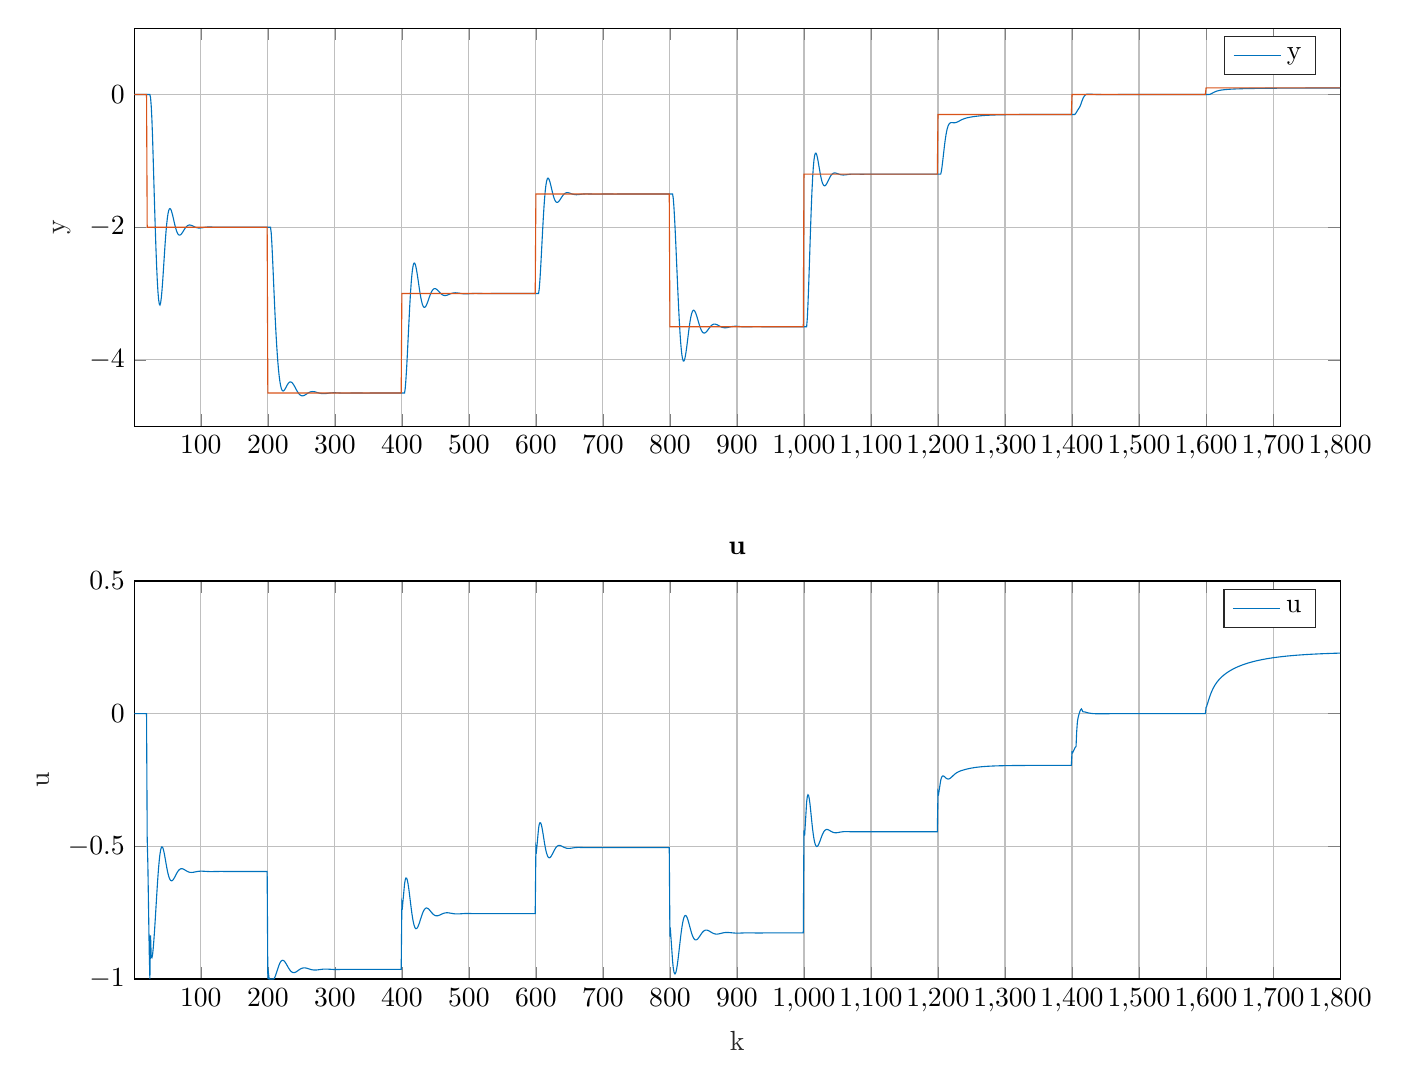
\begin{tikzpicture}

\begin{axis}[%
width=6.028in,
height=1.99in,
at={(1.011in,3.406in)},
scale only axis,
xmin=1,
xmax=1800,
ymin=-5,
ymax=1,
ylabel style={font=\color{white!15!black}},
ylabel={y},
axis background/.style={fill=white},
xmajorgrids,
ymajorgrids,
legend style={legend cell align=left, align=left, draw=white!15!black}
]
\addplot [color=mycolor1]
  table[row sep=crcr]{%
1	0\\
2	0\\
3	0\\
4	0\\
5	0\\
6	0\\
7	0\\
8	0\\
9	0\\
10	0\\
11	0\\
12	0\\
13	0\\
14	0\\
15	0\\
16	0\\
17	0\\
18	0\\
19	0\\
20	0\\
21	0\\
22	0\\
23	0\\
24	0\\
25	-0.046722\\
26	-0.17222\\
27	-0.37125\\
28	-0.64589\\
29	-0.98751\\
30	-1.3387\\
31	-1.6791\\
32	-2.0058\\
33	-2.3073\\
34	-2.5731\\
35	-2.7949\\
36	-2.9676\\
37	-3.0883\\
38	-3.1563\\
39	-3.1729\\
40	-3.1418\\
41	-3.0685\\
42	-2.9604\\
43	-2.8259\\
44	-2.6744\\
45	-2.5154\\
46	-2.3576\\
47	-2.2087\\
48	-2.0748\\
49	-1.9603\\
50	-1.8678\\
51	-1.7982\\
52	-1.7512\\
53	-1.7254\\
54	-1.7186\\
55	-1.7279\\
56	-1.7505\\
57	-1.7831\\
58	-1.8227\\
59	-1.8662\\
60	-1.911\\
61	-1.9547\\
62	-1.9955\\
63	-2.0317\\
64	-2.0622\\
65	-2.0864\\
66	-2.1039\\
67	-2.1146\\
68	-2.1191\\
69	-2.1178\\
70	-2.1116\\
71	-2.1014\\
72	-2.0881\\
73	-2.0729\\
74	-2.0566\\
75	-2.0402\\
76	-2.0245\\
77	-2.01\\
78	-1.9973\\
79	-1.9866\\
80	-1.9783\\
81	-1.9724\\
82	-1.9687\\
83	-1.9671\\
84	-1.9674\\
85	-1.9693\\
86	-1.9725\\
87	-1.9766\\
88	-1.9813\\
89	-1.9863\\
90	-1.9913\\
91	-1.9961\\
92	-2.0004\\
93	-2.0041\\
94	-2.0072\\
95	-2.0095\\
96	-2.0111\\
97	-2.012\\
98	-2.0122\\
99	-2.0118\\
100	-2.0109\\
101	-2.0097\\
102	-2.0082\\
103	-2.0065\\
104	-2.0048\\
105	-2.0031\\
106	-2.0015\\
107	-2.0001\\
108	-1.9989\\
109	-1.9979\\
110	-1.9971\\
111	-1.9966\\
112	-1.9964\\
113	-1.9963\\
114	-1.9965\\
115	-1.9968\\
116	-1.9972\\
117	-1.9976\\
118	-1.9982\\
119	-1.9987\\
120	-1.9993\\
121	-1.9998\\
122	-2.0002\\
123	-2.0006\\
124	-2.0009\\
125	-2.0011\\
126	-2.0012\\
127	-2.0013\\
128	-2.0013\\
129	-2.0012\\
130	-2.0011\\
131	-2.0009\\
132	-2.0008\\
133	-2.0006\\
134	-2.0004\\
135	-2.0002\\
136	-2.0001\\
137	-1.9999\\
138	-1.9998\\
139	-1.9997\\
140	-1.9997\\
141	-1.9996\\
142	-1.9996\\
143	-1.9996\\
144	-1.9996\\
145	-1.9997\\
146	-1.9997\\
147	-1.9998\\
148	-1.9998\\
149	-1.9999\\
150	-1.9999\\
151	-2\\
152	-2\\
153	-2.0001\\
154	-2.0001\\
155	-2.0001\\
156	-2.0001\\
157	-2.0001\\
158	-2.0001\\
159	-2.0001\\
160	-2.0001\\
161	-2.0001\\
162	-2.0001\\
163	-2.0001\\
164	-2\\
165	-2\\
166	-2\\
167	-2\\
168	-2\\
169	-2\\
170	-2\\
171	-2\\
172	-2\\
173	-2\\
174	-2\\
175	-2\\
176	-2\\
177	-2\\
178	-2\\
179	-2\\
180	-2\\
181	-2\\
182	-2\\
183	-2\\
184	-2\\
185	-2\\
186	-2\\
187	-2\\
188	-2\\
189	-2\\
190	-2\\
191	-2\\
192	-2\\
193	-2\\
194	-2\\
195	-2\\
196	-2\\
197	-2\\
198	-2\\
199	-2\\
200	-2\\
201	-2\\
202	-2\\
203	-2\\
204	-2\\
205	-2.0801\\
206	-2.2427\\
207	-2.4526\\
208	-2.6856\\
209	-2.9234\\
210	-3.1541\\
211	-3.3704\\
212	-3.5682\\
213	-3.7459\\
214	-3.903\\
215	-4.0393\\
216	-4.155\\
217	-4.2505\\
218	-4.3267\\
219	-4.3847\\
220	-4.426\\
221	-4.4525\\
222	-4.4661\\
223	-4.4689\\
224	-4.4632\\
225	-4.451\\
226	-4.4346\\
227	-4.4158\\
228	-4.3963\\
229	-4.3778\\
230	-4.3614\\
231	-4.3482\\
232	-4.3387\\
233	-4.3334\\
234	-4.3325\\
235	-4.3358\\
236	-4.3431\\
237	-4.354\\
238	-4.3678\\
239	-4.3839\\
240	-4.4017\\
241	-4.4205\\
242	-4.4394\\
243	-4.458\\
244	-4.4756\\
245	-4.4917\\
246	-4.5059\\
247	-4.5179\\
248	-4.5275\\
249	-4.5347\\
250	-4.5394\\
251	-4.5418\\
252	-4.5419\\
253	-4.5402\\
254	-4.5368\\
255	-4.532\\
256	-4.5263\\
257	-4.52\\
258	-4.5133\\
259	-4.5066\\
260	-4.5002\\
261	-4.4944\\
262	-4.4892\\
263	-4.4849\\
264	-4.4816\\
265	-4.4792\\
266	-4.4779\\
267	-4.4775\\
268	-4.478\\
269	-4.4793\\
270	-4.4812\\
271	-4.4836\\
272	-4.4865\\
273	-4.4895\\
274	-4.4927\\
275	-4.4958\\
276	-4.4988\\
277	-4.5015\\
278	-4.5038\\
279	-4.5058\\
280	-4.5073\\
281	-4.5084\\
282	-4.5091\\
283	-4.5093\\
284	-4.5091\\
285	-4.5086\\
286	-4.5078\\
287	-4.5067\\
288	-4.5055\\
289	-4.5042\\
290	-4.5028\\
291	-4.5015\\
292	-4.5002\\
293	-4.4991\\
294	-4.4981\\
295	-4.4973\\
296	-4.4966\\
297	-4.4962\\
298	-4.4959\\
299	-4.4958\\
300	-4.496\\
301	-4.4962\\
302	-4.4966\\
303	-4.4971\\
304	-4.4976\\
305	-4.4982\\
306	-4.4988\\
307	-4.4994\\
308	-4.4999\\
309	-4.5004\\
310	-4.5009\\
311	-4.5012\\
312	-4.5015\\
313	-4.5017\\
314	-4.5018\\
315	-4.5018\\
316	-4.5018\\
317	-4.5016\\
318	-4.5015\\
319	-4.5013\\
320	-4.501\\
321	-4.5008\\
322	-4.5005\\
323	-4.5003\\
324	-4.5\\
325	-4.4998\\
326	-4.4996\\
327	-4.4995\\
328	-4.4993\\
329	-4.4993\\
330	-4.4992\\
331	-4.4992\\
332	-4.4992\\
333	-4.4993\\
334	-4.4994\\
335	-4.4995\\
336	-4.4996\\
337	-4.4997\\
338	-4.4998\\
339	-4.4999\\
340	-4.5\\
341	-4.5001\\
342	-4.5002\\
343	-4.5002\\
344	-4.5003\\
345	-4.5003\\
346	-4.5003\\
347	-4.5003\\
348	-4.5003\\
349	-4.5003\\
350	-4.5003\\
351	-4.5002\\
352	-4.5002\\
353	-4.5001\\
354	-4.5001\\
355	-4.5\\
356	-4.5\\
357	-4.5\\
358	-4.4999\\
359	-4.4999\\
360	-4.4999\\
361	-4.4999\\
362	-4.4998\\
363	-4.4998\\
364	-4.4999\\
365	-4.4999\\
366	-4.4999\\
367	-4.4999\\
368	-4.4999\\
369	-4.4999\\
370	-4.5\\
371	-4.5\\
372	-4.5\\
373	-4.5\\
374	-4.5\\
375	-4.5\\
376	-4.5001\\
377	-4.5001\\
378	-4.5001\\
379	-4.5001\\
380	-4.5001\\
381	-4.5001\\
382	-4.5001\\
383	-4.5\\
384	-4.5\\
385	-4.5\\
386	-4.5\\
387	-4.5\\
388	-4.5\\
389	-4.5\\
390	-4.5\\
391	-4.5\\
392	-4.5\\
393	-4.5\\
394	-4.5\\
395	-4.5\\
396	-4.5\\
397	-4.5\\
398	-4.5\\
399	-4.5\\
400	-4.5\\
401	-4.5\\
402	-4.5\\
403	-4.5\\
404	-4.5\\
405	-4.4319\\
406	-4.3057\\
407	-4.143\\
408	-3.9553\\
409	-3.7516\\
410	-3.5418\\
411	-3.3365\\
412	-3.1448\\
413	-2.9739\\
414	-2.8288\\
415	-2.7127\\
416	-2.6269\\
417	-2.5708\\
418	-2.5429\\
419	-2.5405\\
420	-2.5601\\
421	-2.598\\
422	-2.65\\
423	-2.7121\\
424	-2.7804\\
425	-2.851\\
426	-2.9208\\
427	-2.9868\\
428	-3.0467\\
429	-3.0985\\
430	-3.1409\\
431	-3.1731\\
432	-3.1949\\
433	-3.2063\\
434	-3.2081\\
435	-3.2012\\
436	-3.1867\\
437	-3.1662\\
438	-3.1412\\
439	-3.1133\\
440	-3.0839\\
441	-3.0545\\
442	-3.0265\\
443	-3.0007\\
444	-2.9781\\
445	-2.9593\\
446	-2.9446\\
447	-2.9341\\
448	-2.9279\\
449	-2.9256\\
450	-2.9268\\
451	-2.9311\\
452	-2.938\\
453	-2.9468\\
454	-2.9569\\
455	-2.9677\\
456	-2.9786\\
457	-2.9893\\
458	-2.9992\\
459	-3.008\\
460	-3.0155\\
461	-3.0215\\
462	-3.0258\\
463	-3.0286\\
464	-3.0298\\
465	-3.0297\\
466	-3.0282\\
467	-3.0258\\
468	-3.0225\\
469	-3.0187\\
470	-3.0145\\
471	-3.0102\\
472	-3.0059\\
473	-3.0019\\
474	-2.9983\\
475	-2.9952\\
476	-2.9927\\
477	-2.9908\\
478	-2.9895\\
479	-2.9888\\
480	-2.9887\\
481	-2.9891\\
482	-2.9899\\
483	-2.9911\\
484	-2.9925\\
485	-2.994\\
486	-2.9957\\
487	-2.9973\\
488	-2.9989\\
489	-3.0003\\
490	-3.0016\\
491	-3.0026\\
492	-3.0034\\
493	-3.004\\
494	-3.0043\\
495	-3.0044\\
496	-3.0043\\
497	-3.004\\
498	-3.0036\\
499	-3.0031\\
500	-3.0025\\
501	-3.0019\\
502	-3.0012\\
503	-3.0006\\
504	-3.0001\\
505	-2.9996\\
506	-2.9991\\
507	-2.9988\\
508	-2.9985\\
509	-2.9984\\
510	-2.9983\\
511	-2.9983\\
512	-2.9984\\
513	-2.9986\\
514	-2.9987\\
515	-2.999\\
516	-2.9992\\
517	-2.9994\\
518	-2.9997\\
519	-2.9999\\
520	-3.0001\\
521	-3.0003\\
522	-3.0004\\
523	-3.0005\\
524	-3.0006\\
525	-3.0006\\
526	-3.0007\\
527	-3.0006\\
528	-3.0006\\
529	-3.0005\\
530	-3.0004\\
531	-3.0003\\
532	-3.0002\\
533	-3.0001\\
534	-3.0001\\
535	-3\\
536	-2.9999\\
537	-2.9998\\
538	-2.9998\\
539	-2.9998\\
540	-2.9998\\
541	-2.9997\\
542	-2.9998\\
543	-2.9998\\
544	-2.9998\\
545	-2.9998\\
546	-2.9999\\
547	-2.9999\\
548	-2.9999\\
549	-3\\
550	-3\\
551	-3\\
552	-3.0001\\
553	-3.0001\\
554	-3.0001\\
555	-3.0001\\
556	-3.0001\\
557	-3.0001\\
558	-3.0001\\
559	-3.0001\\
560	-3.0001\\
561	-3.0001\\
562	-3\\
563	-3\\
564	-3\\
565	-3\\
566	-3\\
567	-3\\
568	-3\\
569	-3\\
570	-3\\
571	-3\\
572	-3\\
573	-3\\
574	-3\\
575	-3\\
576	-3\\
577	-3\\
578	-3\\
579	-3\\
580	-3\\
581	-3\\
582	-3\\
583	-3\\
584	-3\\
585	-3\\
586	-3\\
587	-3\\
588	-3\\
589	-3\\
590	-3\\
591	-3\\
592	-3\\
593	-3\\
594	-3\\
595	-3\\
596	-3\\
597	-3\\
598	-3\\
599	-3\\
600	-3\\
601	-3\\
602	-3\\
603	-3\\
604	-3\\
605	-2.9262\\
606	-2.7955\\
607	-2.631\\
608	-2.4459\\
609	-2.2501\\
610	-2.0544\\
611	-1.8697\\
612	-1.704\\
613	-1.5627\\
614	-1.4488\\
615	-1.363\\
616	-1.3044\\
617	-1.2709\\
618	-1.2593\\
619	-1.266\\
620	-1.2872\\
621	-1.3192\\
622	-1.3582\\
623	-1.401\\
624	-1.4446\\
625	-1.4866\\
626	-1.5249\\
627	-1.558\\
628	-1.5849\\
629	-1.6051\\
630	-1.6185\\
631	-1.6252\\
632	-1.6259\\
633	-1.6214\\
634	-1.6125\\
635	-1.6003\\
636	-1.5858\\
637	-1.5701\\
638	-1.5541\\
639	-1.5386\\
640	-1.5242\\
641	-1.5115\\
642	-1.5007\\
643	-1.4921\\
644	-1.4858\\
645	-1.4815\\
646	-1.4792\\
647	-1.4787\\
648	-1.4796\\
649	-1.4816\\
650	-1.4845\\
651	-1.488\\
652	-1.4917\\
653	-1.4954\\
654	-1.4989\\
655	-1.502\\
656	-1.5047\\
657	-1.5069\\
658	-1.5084\\
659	-1.5094\\
660	-1.5099\\
661	-1.5098\\
662	-1.5094\\
663	-1.5086\\
664	-1.5076\\
665	-1.5064\\
666	-1.5051\\
667	-1.5039\\
668	-1.5026\\
669	-1.5015\\
670	-1.5005\\
671	-1.4997\\
672	-1.4991\\
673	-1.4986\\
674	-1.4983\\
675	-1.4982\\
676	-1.4982\\
677	-1.4983\\
678	-1.4985\\
679	-1.4987\\
680	-1.499\\
681	-1.4993\\
682	-1.4996\\
683	-1.4999\\
684	-1.5002\\
685	-1.5004\\
686	-1.5006\\
687	-1.5007\\
688	-1.5007\\
689	-1.5008\\
690	-1.5008\\
691	-1.5007\\
692	-1.5007\\
693	-1.5006\\
694	-1.5005\\
695	-1.5004\\
696	-1.5003\\
697	-1.5002\\
698	-1.5001\\
699	-1.5\\
700	-1.5\\
701	-1.4999\\
702	-1.4999\\
703	-1.4999\\
704	-1.4998\\
705	-1.4998\\
706	-1.4999\\
707	-1.4999\\
708	-1.4999\\
709	-1.4999\\
710	-1.4999\\
711	-1.5\\
712	-1.5\\
713	-1.5\\
714	-1.5\\
715	-1.5\\
716	-1.5001\\
717	-1.5001\\
718	-1.5001\\
719	-1.5001\\
720	-1.5001\\
721	-1.5001\\
722	-1.5\\
723	-1.5\\
724	-1.5\\
725	-1.5\\
726	-1.5\\
727	-1.5\\
728	-1.5\\
729	-1.5\\
730	-1.5\\
731	-1.5\\
732	-1.5\\
733	-1.5\\
734	-1.5\\
735	-1.5\\
736	-1.5\\
737	-1.5\\
738	-1.5\\
739	-1.5\\
740	-1.5\\
741	-1.5\\
742	-1.5\\
743	-1.5\\
744	-1.5\\
745	-1.5\\
746	-1.5\\
747	-1.5\\
748	-1.5\\
749	-1.5\\
750	-1.5\\
751	-1.5\\
752	-1.5\\
753	-1.5\\
754	-1.5\\
755	-1.5\\
756	-1.5\\
757	-1.5\\
758	-1.5\\
759	-1.5\\
760	-1.5\\
761	-1.5\\
762	-1.5\\
763	-1.5\\
764	-1.5\\
765	-1.5\\
766	-1.5\\
767	-1.5\\
768	-1.5\\
769	-1.5\\
770	-1.5\\
771	-1.5\\
772	-1.5\\
773	-1.5\\
774	-1.5\\
775	-1.5\\
776	-1.5\\
777	-1.5\\
778	-1.5\\
779	-1.5\\
780	-1.5\\
781	-1.5\\
782	-1.5\\
783	-1.5\\
784	-1.5\\
785	-1.5\\
786	-1.5\\
787	-1.5\\
788	-1.5\\
789	-1.5\\
790	-1.5\\
791	-1.5\\
792	-1.5\\
793	-1.5\\
794	-1.5\\
795	-1.5\\
796	-1.5\\
797	-1.5\\
798	-1.5\\
799	-1.5\\
800	-1.5\\
801	-1.5\\
802	-1.5\\
803	-1.5\\
804	-1.5\\
805	-1.567\\
806	-1.7013\\
807	-1.877\\
808	-2.0809\\
809	-2.3039\\
810	-2.5375\\
811	-2.7728\\
812	-3.0019\\
813	-3.2178\\
814	-3.4145\\
815	-3.5876\\
816	-3.7335\\
817	-3.8499\\
818	-3.9358\\
819	-3.9911\\
820	-4.0172\\
821	-4.0161\\
822	-3.9909\\
823	-3.9454\\
824	-3.8839\\
825	-3.8108\\
826	-3.7307\\
827	-3.6481\\
828	-3.5669\\
829	-3.4908\\
830	-3.4227\\
831	-3.3645\\
832	-3.3179\\
833	-3.2836\\
834	-3.2617\\
835	-3.2518\\
836	-3.2529\\
837	-3.2638\\
838	-3.283\\
839	-3.3087\\
840	-3.3393\\
841	-3.3729\\
842	-3.4078\\
843	-3.4426\\
844	-3.4758\\
845	-3.5062\\
846	-3.533\\
847	-3.5554\\
848	-3.573\\
849	-3.5856\\
850	-3.5932\\
851	-3.596\\
852	-3.5945\\
853	-3.5892\\
854	-3.5807\\
855	-3.5697\\
856	-3.5569\\
857	-3.5432\\
858	-3.5291\\
859	-3.5153\\
860	-3.5024\\
861	-3.4908\\
862	-3.4808\\
863	-3.4727\\
864	-3.4666\\
865	-3.4626\\
866	-3.4605\\
867	-3.4604\\
868	-3.4619\\
869	-3.4648\\
870	-3.4688\\
871	-3.4737\\
872	-3.4792\\
873	-3.4849\\
874	-3.4906\\
875	-3.4961\\
876	-3.5011\\
877	-3.5056\\
878	-3.5093\\
879	-3.5122\\
880	-3.5143\\
881	-3.5156\\
882	-3.5161\\
883	-3.5159\\
884	-3.515\\
885	-3.5136\\
886	-3.5118\\
887	-3.5096\\
888	-3.5074\\
889	-3.505\\
890	-3.5027\\
891	-3.5006\\
892	-3.4986\\
893	-3.497\\
894	-3.4956\\
895	-3.4946\\
896	-3.4939\\
897	-3.4935\\
898	-3.4935\\
899	-3.4937\\
900	-3.4941\\
901	-3.4948\\
902	-3.4956\\
903	-3.4965\\
904	-3.4974\\
905	-3.4984\\
906	-3.4993\\
907	-3.5001\\
908	-3.5009\\
909	-3.5015\\
910	-3.502\\
911	-3.5024\\
912	-3.5026\\
913	-3.5027\\
914	-3.5026\\
915	-3.5025\\
916	-3.5023\\
917	-3.502\\
918	-3.5016\\
919	-3.5012\\
920	-3.5009\\
921	-3.5005\\
922	-3.5001\\
923	-3.4998\\
924	-3.4995\\
925	-3.4993\\
926	-3.4991\\
927	-3.499\\
928	-3.4989\\
929	-3.4989\\
930	-3.4989\\
931	-3.499\\
932	-3.4991\\
933	-3.4993\\
934	-3.4994\\
935	-3.4996\\
936	-3.4997\\
937	-3.4999\\
938	-3.5\\
939	-3.5001\\
940	-3.5002\\
941	-3.5003\\
942	-3.5004\\
943	-3.5004\\
944	-3.5004\\
945	-3.5004\\
946	-3.5004\\
947	-3.5004\\
948	-3.5003\\
949	-3.5003\\
950	-3.5002\\
951	-3.5001\\
952	-3.5001\\
953	-3.5\\
954	-3.5\\
955	-3.4999\\
956	-3.4999\\
957	-3.4999\\
958	-3.4998\\
959	-3.4998\\
960	-3.4998\\
961	-3.4998\\
962	-3.4998\\
963	-3.4999\\
964	-3.4999\\
965	-3.4999\\
966	-3.4999\\
967	-3.5\\
968	-3.5\\
969	-3.5\\
970	-3.5\\
971	-3.5\\
972	-3.5001\\
973	-3.5001\\
974	-3.5001\\
975	-3.5001\\
976	-3.5001\\
977	-3.5001\\
978	-3.5001\\
979	-3.5001\\
980	-3.5\\
981	-3.5\\
982	-3.5\\
983	-3.5\\
984	-3.5\\
985	-3.5\\
986	-3.5\\
987	-3.5\\
988	-3.5\\
989	-3.5\\
990	-3.5\\
991	-3.5\\
992	-3.5\\
993	-3.5\\
994	-3.5\\
995	-3.5\\
996	-3.5\\
997	-3.5\\
998	-3.5\\
999	-3.5\\
1000	-3.5\\
1001	-3.5\\
1002	-3.5\\
1003	-3.5\\
1004	-3.5\\
1005	-3.3746\\
1006	-3.1592\\
1007	-2.8907\\
1008	-2.5911\\
1009	-2.2772\\
1010	-1.9699\\
1011	-1.6876\\
1012	-1.4432\\
1013	-1.2434\\
1014	-1.0904\\
1015	-0.98243\\
1016	-0.91576\\
1017	-0.88498\\
1018	-0.88403\\
1019	-0.90662\\
1020	-0.94665\\
1021	-0.9984\\
1022	-1.0567\\
1023	-1.1171\\
1024	-1.1757\\
1025	-1.2296\\
1026	-1.2766\\
1027	-1.315\\
1028	-1.344\\
1029	-1.3635\\
1030	-1.3737\\
1031	-1.3755\\
1032	-1.3699\\
1033	-1.3582\\
1034	-1.3421\\
1035	-1.3229\\
1036	-1.3021\\
1037	-1.2809\\
1038	-1.2605\\
1039	-1.2416\\
1040	-1.225\\
1041	-1.211\\
1042	-1.1999\\
1043	-1.1916\\
1044	-1.1861\\
1045	-1.183\\
1046	-1.182\\
1047	-1.1828\\
1048	-1.1849\\
1049	-1.1879\\
1050	-1.1915\\
1051	-1.1954\\
1052	-1.1992\\
1053	-1.2028\\
1054	-1.2059\\
1055	-1.2084\\
1056	-1.2103\\
1057	-1.2116\\
1058	-1.2123\\
1059	-1.2124\\
1060	-1.212\\
1061	-1.2112\\
1062	-1.2102\\
1063	-1.2089\\
1064	-1.2075\\
1065	-1.2061\\
1066	-1.2047\\
1067	-1.2035\\
1068	-1.2023\\
1069	-1.2014\\
1070	-1.2006\\
1071	-1.2\\
1072	-1.1996\\
1073	-1.1993\\
1074	-1.1992\\
1075	-1.1992\\
1076	-1.1993\\
1077	-1.1994\\
1078	-1.1996\\
1079	-1.1999\\
1080	-1.2001\\
1081	-1.2003\\
1082	-1.2005\\
1083	-1.2006\\
1084	-1.2008\\
1085	-1.2008\\
1086	-1.2009\\
1087	-1.2009\\
1088	-1.2009\\
1089	-1.2008\\
1090	-1.2007\\
1091	-1.2007\\
1092	-1.2006\\
1093	-1.2005\\
1094	-1.2004\\
1095	-1.2003\\
1096	-1.2002\\
1097	-1.2001\\
1098	-1.2001\\
1099	-1.2\\
1100	-1.2\\
1101	-1.2\\
1102	-1.2\\
1103	-1.2\\
1104	-1.2\\
1105	-1.2\\
1106	-1.2\\
1107	-1.2\\
1108	-1.2\\
1109	-1.2\\
1110	-1.2\\
1111	-1.2001\\
1112	-1.2001\\
1113	-1.2001\\
1114	-1.2001\\
1115	-1.2001\\
1116	-1.2001\\
1117	-1.2001\\
1118	-1.2001\\
1119	-1.2\\
1120	-1.2\\
1121	-1.2\\
1122	-1.2\\
1123	-1.2\\
1124	-1.2\\
1125	-1.2\\
1126	-1.2\\
1127	-1.2\\
1128	-1.2\\
1129	-1.2\\
1130	-1.2\\
1131	-1.2\\
1132	-1.2\\
1133	-1.2\\
1134	-1.2\\
1135	-1.2\\
1136	-1.2\\
1137	-1.2\\
1138	-1.2\\
1139	-1.2\\
1140	-1.2\\
1141	-1.2\\
1142	-1.2\\
1143	-1.2\\
1144	-1.2\\
1145	-1.2\\
1146	-1.2\\
1147	-1.2\\
1148	-1.2\\
1149	-1.2\\
1150	-1.2\\
1151	-1.2\\
1152	-1.2\\
1153	-1.2\\
1154	-1.2\\
1155	-1.2\\
1156	-1.2\\
1157	-1.2\\
1158	-1.2\\
1159	-1.2\\
1160	-1.2\\
1161	-1.2\\
1162	-1.2\\
1163	-1.2\\
1164	-1.2\\
1165	-1.2\\
1166	-1.2\\
1167	-1.2\\
1168	-1.2\\
1169	-1.2\\
1170	-1.2\\
1171	-1.2\\
1172	-1.2\\
1173	-1.2\\
1174	-1.2\\
1175	-1.2\\
1176	-1.2\\
1177	-1.2\\
1178	-1.2\\
1179	-1.2\\
1180	-1.2\\
1181	-1.2\\
1182	-1.2\\
1183	-1.2\\
1184	-1.2\\
1185	-1.2\\
1186	-1.2\\
1187	-1.2\\
1188	-1.2\\
1189	-1.2\\
1190	-1.2\\
1191	-1.2\\
1192	-1.2\\
1193	-1.2\\
1194	-1.2\\
1195	-1.2\\
1196	-1.2\\
1197	-1.2\\
1198	-1.2\\
1199	-1.2\\
1200	-1.2\\
1201	-1.2\\
1202	-1.2\\
1203	-1.2\\
1204	-1.2\\
1205	-1.1595\\
1206	-1.0904\\
1207	-1.0075\\
1208	-0.91874\\
1209	-0.82958\\
1210	-0.7449\\
1211	-0.66863\\
1212	-0.60311\\
1213	-0.54926\\
1214	-0.50692\\
1215	-0.4752\\
1216	-0.45274\\
1217	-0.43794\\
1218	-0.42911\\
1219	-0.42465\\
1220	-0.42312\\
1221	-0.42329\\
1222	-0.42418\\
1223	-0.42504\\
1224	-0.42536\\
1225	-0.42481\\
1226	-0.42326\\
1227	-0.4207\\
1228	-0.41721\\
1229	-0.41295\\
1230	-0.40811\\
1231	-0.40289\\
1232	-0.39746\\
1233	-0.392\\
1234	-0.38665\\
1235	-0.38152\\
1236	-0.37667\\
1237	-0.37216\\
1238	-0.36799\\
1239	-0.36418\\
1240	-0.3607\\
1241	-0.35754\\
1242	-0.35465\\
1243	-0.352\\
1244	-0.34956\\
1245	-0.34729\\
1246	-0.34517\\
1247	-0.34318\\
1248	-0.34129\\
1249	-0.33949\\
1250	-0.33777\\
1251	-0.33611\\
1252	-0.33452\\
1253	-0.33299\\
1254	-0.33152\\
1255	-0.33011\\
1256	-0.32875\\
1257	-0.32745\\
1258	-0.3262\\
1259	-0.32501\\
1260	-0.32388\\
1261	-0.32279\\
1262	-0.32176\\
1263	-0.32077\\
1264	-0.31984\\
1265	-0.31895\\
1266	-0.3181\\
1267	-0.31729\\
1268	-0.31651\\
1269	-0.31578\\
1270	-0.31508\\
1271	-0.31441\\
1272	-0.31377\\
1273	-0.31316\\
1274	-0.31258\\
1275	-0.31203\\
1276	-0.3115\\
1277	-0.31099\\
1278	-0.31051\\
1279	-0.31005\\
1280	-0.3096\\
1281	-0.30918\\
1282	-0.30878\\
1283	-0.30839\\
1284	-0.30802\\
1285	-0.30767\\
1286	-0.30733\\
1287	-0.30701\\
1288	-0.30671\\
1289	-0.30641\\
1290	-0.30613\\
1291	-0.30586\\
1292	-0.30561\\
1293	-0.30536\\
1294	-0.30513\\
1295	-0.3049\\
1296	-0.30469\\
1297	-0.30448\\
1298	-0.30429\\
1299	-0.3041\\
1300	-0.30392\\
1301	-0.30375\\
1302	-0.30359\\
1303	-0.30343\\
1304	-0.30328\\
1305	-0.30314\\
1306	-0.303\\
1307	-0.30287\\
1308	-0.30275\\
1309	-0.30263\\
1310	-0.30251\\
1311	-0.3024\\
1312	-0.3023\\
1313	-0.3022\\
1314	-0.3021\\
1315	-0.30201\\
1316	-0.30192\\
1317	-0.30184\\
1318	-0.30176\\
1319	-0.30168\\
1320	-0.30161\\
1321	-0.30154\\
1322	-0.30147\\
1323	-0.30141\\
1324	-0.30135\\
1325	-0.30129\\
1326	-0.30123\\
1327	-0.30118\\
1328	-0.30113\\
1329	-0.30108\\
1330	-0.30103\\
1331	-0.30099\\
1332	-0.30095\\
1333	-0.3009\\
1334	-0.30087\\
1335	-0.30083\\
1336	-0.30079\\
1337	-0.30076\\
1338	-0.30072\\
1339	-0.30069\\
1340	-0.30066\\
1341	-0.30063\\
1342	-0.30061\\
1343	-0.30058\\
1344	-0.30056\\
1345	-0.30053\\
1346	-0.30051\\
1347	-0.30049\\
1348	-0.30046\\
1349	-0.30044\\
1350	-0.30043\\
1351	-0.30041\\
1352	-0.30039\\
1353	-0.30037\\
1354	-0.30036\\
1355	-0.30034\\
1356	-0.30033\\
1357	-0.30031\\
1358	-0.3003\\
1359	-0.30029\\
1360	-0.30027\\
1361	-0.30026\\
1362	-0.30025\\
1363	-0.30024\\
1364	-0.30023\\
1365	-0.30022\\
1366	-0.30021\\
1367	-0.3002\\
1368	-0.30019\\
1369	-0.30018\\
1370	-0.30018\\
1371	-0.30017\\
1372	-0.30016\\
1373	-0.30015\\
1374	-0.30015\\
1375	-0.30014\\
1376	-0.30013\\
1377	-0.30013\\
1378	-0.30012\\
1379	-0.30012\\
1380	-0.30011\\
1381	-0.30011\\
1382	-0.3001\\
1383	-0.3001\\
1384	-0.30009\\
1385	-0.30009\\
1386	-0.30009\\
1387	-0.30008\\
1388	-0.30008\\
1389	-0.30008\\
1390	-0.30007\\
1391	-0.30007\\
1392	-0.30007\\
1393	-0.30006\\
1394	-0.30006\\
1395	-0.30006\\
1396	-0.30006\\
1397	-0.30005\\
1398	-0.30005\\
1399	-0.30005\\
1400	-0.30005\\
1401	-0.30004\\
1402	-0.30004\\
1403	-0.30004\\
1404	-0.30004\\
1405	-0.2917\\
1406	-0.27707\\
1407	-0.26021\\
1408	-0.24291\\
1409	-0.22617\\
1410	-0.21067\\
1411	-0.19685\\
1412	-0.17785\\
1413	-0.15151\\
1414	-0.12184\\
1415	-0.093042\\
1416	-0.067422\\
1417	-0.045827\\
1418	-0.028371\\
1419	-0.014777\\
1420	-0.0048728\\
1421	0.0014373\\
1422	0.0048604\\
1423	0.00648\\
1424	0.0070753\\
1425	0.0070758\\
1426	0.0067294\\
1427	0.0061924\\
1428	0.005566\\
1429	0.0049132\\
1430	0.0042715\\
1431	0.0036628\\
1432	0.0030994\\
1433	0.0025874\\
1434	0.0021286\\
1435	0.0017228\\
1436	0.0013677\\
1437	0.0010605\\
1438	0.00079754\\
1439	0.00057494\\
1440	0.00038876\\
1441	0.00023511\\
1442	0.00011021\\
1443	1.0491e-05\\
1444	-6.7409e-05\\
1445	-0.00012658\\
1446	-0.00016985\\
1447	-0.00019977\\
1448	-0.00021863\\
1449	-0.00022845\\
1450	-0.00023101\\
1451	-0.00022787\\
1452	-0.00022036\\
1453	-0.0002096\\
1454	-0.00019657\\
1455	-0.00018204\\
1456	-0.00016668\\
1457	-0.00015101\\
1458	-0.00013545\\
1459	-0.00012032\\
1460	-0.00010586\\
1461	-9.2254e-05\\
1462	-7.9605e-05\\
1463	-6.7987e-05\\
1464	-5.7429e-05\\
1465	-4.7931e-05\\
1466	-3.9471e-05\\
1467	-3.2006e-05\\
1468	-2.5483e-05\\
1469	-1.9837e-05\\
1470	-1.5001e-05\\
1471	-1.0902e-05\\
1472	-7.4679e-06\\
1473	-4.6285e-06\\
1474	-2.315e-06\\
1475	-4.6227e-07\\
1476	9.9047e-07\\
1477	2.0995e-06\\
1478	2.9163e-06\\
1479	3.4875e-06\\
1480	3.8546e-06\\
1481	4.0548e-06\\
1482	4.1205e-06\\
1483	4.0801e-06\\
1484	3.958e-06\\
1485	3.7749e-06\\
1486	3.5485e-06\\
1487	3.2934e-06\\
1488	3.0215e-06\\
1489	2.7427e-06\\
1490	2.4647e-06\\
1491	2.1934e-06\\
1492	1.9335e-06\\
1493	1.6882e-06\\
1494	1.4596e-06\\
1495	1.2492e-06\\
1496	1.0577e-06\\
1497	8.8504e-07\\
1498	7.3095e-07\\
1499	5.9474e-07\\
1500	4.7547e-07\\
1501	3.7204e-07\\
1502	2.8325e-07\\
1503	2.0782e-07\\
1504	1.4448e-07\\
1505	9.1946e-08\\
1506	4.9005e-08\\
1507	1.4483e-08\\
1508	-1.2716e-08\\
1509	-3.361e-08\\
1510	-4.9131e-08\\
1511	-6.0122e-08\\
1512	-6.7344e-08\\
1513	-7.147e-08\\
1514	-7.3093e-08\\
1515	-7.2733e-08\\
1516	-7.0836e-08\\
1517	-6.7784e-08\\
1518	-6.3902e-08\\
1519	-5.9459e-08\\
1520	-5.4678e-08\\
1521	-4.9741e-08\\
1522	-4.4792e-08\\
1523	-3.9942e-08\\
1524	-3.5279e-08\\
1525	-3.0865e-08\\
1526	-2.6742e-08\\
1527	-2.2937e-08\\
1528	-1.9465e-08\\
1529	-1.633e-08\\
1530	-1.3525e-08\\
1531	-1.1041e-08\\
1532	-8.862e-09\\
1533	-6.9683e-09\\
1534	-5.339e-09\\
1535	-3.9518e-09\\
1536	-2.784e-09\\
1537	-1.8129e-09\\
1538	-1.0165e-09\\
1539	-3.7391e-10\\
1540	1.3472e-10\\
1541	5.2774e-10\\
1542	8.22e-10\\
1543	1.0328e-09\\
1544	1.174e-09\\
1545	1.2579e-09\\
1546	1.2952e-09\\
1547	1.2954e-09\\
1548	1.2668e-09\\
1549	1.2164e-09\\
1550	1.1501e-09\\
1551	1.073e-09\\
1552	9.8904e-10\\
1553	9.0172e-10\\
1554	8.1368e-10\\
1555	7.2706e-10\\
1556	6.4346e-10\\
1557	5.6407e-10\\
1558	4.8972e-10\\
1559	4.2095e-10\\
1560	3.5805e-10\\
1561	3.0112e-10\\
1562	2.5011e-10\\
1563	2.0483e-10\\
1564	1.6503e-10\\
1565	1.3037e-10\\
1566	1.0049e-10\\
1567	7.4988e-11\\
1568	5.347e-11\\
1569	3.5528e-11\\
1570	2.0769e-11\\
1571	8.8164e-12\\
1572	-6.8526e-13\\
1573	-8.0677e-12\\
1574	-1.3636e-11\\
1575	-1.7669e-11\\
1576	-2.0415e-11\\
1577	-2.21e-11\\
1578	-2.2921e-11\\
1579	-2.305e-11\\
1580	-2.2638e-11\\
1581	-2.1815e-11\\
1582	-2.0689e-11\\
1583	-1.9352e-11\\
1584	-1.7882e-11\\
1585	-1.6339e-11\\
1586	-1.4775e-11\\
1587	-1.3229e-11\\
1588	-1.1731e-11\\
1589	-1.0304e-11\\
1590	-8.9643e-12\\
1591	-7.7219e-12\\
1592	-6.5829e-12\\
1593	-5.5498e-12\\
1594	-4.6221e-12\\
1595	-3.7972e-12\\
1596	-3.0705e-12\\
1597	-2.4364e-12\\
1598	-1.8886e-12\\
1599	-1.4202e-12\\
1600	-1.0239e-12\\
1601	-6.9257e-13\\
1602	-4.1924e-13\\
1603	-1.9711e-13\\
1604	-1.9789e-14\\
1605	0.0014818\\
1606	0.0049077\\
1607	0.00936\\
1608	0.014417\\
1609	0.019762\\
1610	0.025159\\
1611	0.030424\\
1612	0.035423\\
1613	0.040075\\
1614	0.044339\\
1615	0.048206\\
1616	0.051687\\
1617	0.054804\\
1618	0.05759\\
1619	0.060079\\
1620	0.062306\\
1621	0.064303\\
1622	0.0661\\
1623	0.067725\\
1624	0.069201\\
1625	0.070547\\
1626	0.071782\\
1627	0.07292\\
1628	0.073972\\
1629	0.07495\\
1630	0.075862\\
1631	0.076716\\
1632	0.077517\\
1633	0.07827\\
1634	0.078982\\
1635	0.079655\\
1636	0.080292\\
1637	0.080897\\
1638	0.081472\\
1639	0.08202\\
1640	0.082543\\
1641	0.083042\\
1642	0.083519\\
1643	0.083976\\
1644	0.084413\\
1645	0.084833\\
1646	0.085235\\
1647	0.085622\\
1648	0.085994\\
1649	0.086352\\
1650	0.086696\\
1651	0.087028\\
1652	0.087348\\
1653	0.087657\\
1654	0.087955\\
1655	0.088243\\
1656	0.088522\\
1657	0.088791\\
1658	0.089051\\
1659	0.089303\\
1660	0.089547\\
1661	0.089783\\
1662	0.090012\\
1663	0.090235\\
1664	0.09045\\
1665	0.090659\\
1666	0.090862\\
1667	0.091059\\
1668	0.091251\\
1669	0.091437\\
1670	0.091618\\
1671	0.091793\\
1672	0.091964\\
1673	0.092131\\
1674	0.092293\\
1675	0.09245\\
1676	0.092604\\
1677	0.092753\\
1678	0.092899\\
1679	0.093041\\
1680	0.093179\\
1681	0.093314\\
1682	0.093446\\
1683	0.093574\\
1684	0.093699\\
1685	0.093821\\
1686	0.09394\\
1687	0.094057\\
1688	0.09417\\
1689	0.094281\\
1690	0.094389\\
1691	0.094495\\
1692	0.094599\\
1693	0.0947\\
1694	0.094798\\
1695	0.094895\\
1696	0.094989\\
1697	0.095081\\
1698	0.095172\\
1699	0.09526\\
1700	0.095346\\
1701	0.095431\\
1702	0.095513\\
1703	0.095594\\
1704	0.095673\\
1705	0.095751\\
1706	0.095827\\
1707	0.095901\\
1708	0.095974\\
1709	0.096045\\
1710	0.096115\\
1711	0.096183\\
1712	0.09625\\
1713	0.096315\\
1714	0.09638\\
1715	0.096443\\
1716	0.096504\\
1717	0.096565\\
1718	0.096624\\
1719	0.096682\\
1720	0.096739\\
1721	0.096795\\
1722	0.09685\\
1723	0.096903\\
1724	0.096956\\
1725	0.097008\\
1726	0.097058\\
1727	0.097108\\
1728	0.097157\\
1729	0.097205\\
1730	0.097252\\
1731	0.097298\\
1732	0.097343\\
1733	0.097387\\
1734	0.097431\\
1735	0.097474\\
1736	0.097515\\
1737	0.097557\\
1738	0.097597\\
1739	0.097637\\
1740	0.097676\\
1741	0.097714\\
1742	0.097751\\
1743	0.097788\\
1744	0.097825\\
1745	0.09786\\
1746	0.097895\\
1747	0.097929\\
1748	0.097963\\
1749	0.097996\\
1750	0.098029\\
1751	0.098061\\
1752	0.098092\\
1753	0.098123\\
1754	0.098153\\
1755	0.098183\\
1756	0.098212\\
1757	0.098241\\
1758	0.098269\\
1759	0.098297\\
1760	0.098324\\
1761	0.098351\\
1762	0.098377\\
1763	0.098403\\
1764	0.098429\\
1765	0.098454\\
1766	0.098478\\
1767	0.098502\\
1768	0.098526\\
1769	0.09855\\
1770	0.098573\\
1771	0.098595\\
1772	0.098617\\
1773	0.098639\\
1774	0.098661\\
1775	0.098682\\
1776	0.098702\\
1777	0.098723\\
1778	0.098743\\
1779	0.098763\\
1780	0.098782\\
1781	0.098801\\
1782	0.09882\\
1783	0.098838\\
1784	0.098857\\
1785	0.098874\\
1786	0.098892\\
1787	0.098909\\
1788	0.098926\\
1789	0.098943\\
1790	0.098959\\
1791	0.098976\\
1792	0.098991\\
1793	0.099007\\
1794	0.099023\\
1795	0.099038\\
1796	0.099053\\
1797	0.099067\\
1798	0.099082\\
1799	0.099096\\
1800	0.09911\\
};
\addlegendentry{y}

\addplot [color=mycolor2, forget plot]
  table[row sep=crcr]{%
1	0\\
2	0\\
3	0\\
4	0\\
5	0\\
6	0\\
7	0\\
8	0\\
9	0\\
10	0\\
11	0\\
12	0\\
13	0\\
14	0\\
15	0\\
16	0\\
17	0\\
18	0\\
19	0\\
20	-2\\
21	-2\\
22	-2\\
23	-2\\
24	-2\\
25	-2\\
26	-2\\
27	-2\\
28	-2\\
29	-2\\
30	-2\\
31	-2\\
32	-2\\
33	-2\\
34	-2\\
35	-2\\
36	-2\\
37	-2\\
38	-2\\
39	-2\\
40	-2\\
41	-2\\
42	-2\\
43	-2\\
44	-2\\
45	-2\\
46	-2\\
47	-2\\
48	-2\\
49	-2\\
50	-2\\
51	-2\\
52	-2\\
53	-2\\
54	-2\\
55	-2\\
56	-2\\
57	-2\\
58	-2\\
59	-2\\
60	-2\\
61	-2\\
62	-2\\
63	-2\\
64	-2\\
65	-2\\
66	-2\\
67	-2\\
68	-2\\
69	-2\\
70	-2\\
71	-2\\
72	-2\\
73	-2\\
74	-2\\
75	-2\\
76	-2\\
77	-2\\
78	-2\\
79	-2\\
80	-2\\
81	-2\\
82	-2\\
83	-2\\
84	-2\\
85	-2\\
86	-2\\
87	-2\\
88	-2\\
89	-2\\
90	-2\\
91	-2\\
92	-2\\
93	-2\\
94	-2\\
95	-2\\
96	-2\\
97	-2\\
98	-2\\
99	-2\\
100	-2\\
101	-2\\
102	-2\\
103	-2\\
104	-2\\
105	-2\\
106	-2\\
107	-2\\
108	-2\\
109	-2\\
110	-2\\
111	-2\\
112	-2\\
113	-2\\
114	-2\\
115	-2\\
116	-2\\
117	-2\\
118	-2\\
119	-2\\
120	-2\\
121	-2\\
122	-2\\
123	-2\\
124	-2\\
125	-2\\
126	-2\\
127	-2\\
128	-2\\
129	-2\\
130	-2\\
131	-2\\
132	-2\\
133	-2\\
134	-2\\
135	-2\\
136	-2\\
137	-2\\
138	-2\\
139	-2\\
140	-2\\
141	-2\\
142	-2\\
143	-2\\
144	-2\\
145	-2\\
146	-2\\
147	-2\\
148	-2\\
149	-2\\
150	-2\\
151	-2\\
152	-2\\
153	-2\\
154	-2\\
155	-2\\
156	-2\\
157	-2\\
158	-2\\
159	-2\\
160	-2\\
161	-2\\
162	-2\\
163	-2\\
164	-2\\
165	-2\\
166	-2\\
167	-2\\
168	-2\\
169	-2\\
170	-2\\
171	-2\\
172	-2\\
173	-2\\
174	-2\\
175	-2\\
176	-2\\
177	-2\\
178	-2\\
179	-2\\
180	-2\\
181	-2\\
182	-2\\
183	-2\\
184	-2\\
185	-2\\
186	-2\\
187	-2\\
188	-2\\
189	-2\\
190	-2\\
191	-2\\
192	-2\\
193	-2\\
194	-2\\
195	-2\\
196	-2\\
197	-2\\
198	-2\\
199	-2\\
200	-4.5\\
201	-4.5\\
202	-4.5\\
203	-4.5\\
204	-4.5\\
205	-4.5\\
206	-4.5\\
207	-4.5\\
208	-4.5\\
209	-4.5\\
210	-4.5\\
211	-4.5\\
212	-4.5\\
213	-4.5\\
214	-4.5\\
215	-4.5\\
216	-4.5\\
217	-4.5\\
218	-4.5\\
219	-4.5\\
220	-4.5\\
221	-4.5\\
222	-4.5\\
223	-4.5\\
224	-4.5\\
225	-4.5\\
226	-4.5\\
227	-4.5\\
228	-4.5\\
229	-4.5\\
230	-4.5\\
231	-4.5\\
232	-4.5\\
233	-4.5\\
234	-4.5\\
235	-4.5\\
236	-4.5\\
237	-4.5\\
238	-4.5\\
239	-4.5\\
240	-4.5\\
241	-4.5\\
242	-4.5\\
243	-4.5\\
244	-4.5\\
245	-4.5\\
246	-4.5\\
247	-4.5\\
248	-4.5\\
249	-4.5\\
250	-4.5\\
251	-4.5\\
252	-4.5\\
253	-4.5\\
254	-4.5\\
255	-4.5\\
256	-4.5\\
257	-4.5\\
258	-4.5\\
259	-4.5\\
260	-4.5\\
261	-4.5\\
262	-4.5\\
263	-4.5\\
264	-4.5\\
265	-4.5\\
266	-4.5\\
267	-4.5\\
268	-4.5\\
269	-4.5\\
270	-4.5\\
271	-4.5\\
272	-4.5\\
273	-4.5\\
274	-4.5\\
275	-4.5\\
276	-4.5\\
277	-4.5\\
278	-4.5\\
279	-4.5\\
280	-4.5\\
281	-4.5\\
282	-4.5\\
283	-4.5\\
284	-4.5\\
285	-4.5\\
286	-4.5\\
287	-4.5\\
288	-4.5\\
289	-4.5\\
290	-4.5\\
291	-4.5\\
292	-4.5\\
293	-4.5\\
294	-4.5\\
295	-4.5\\
296	-4.5\\
297	-4.5\\
298	-4.5\\
299	-4.5\\
300	-4.5\\
301	-4.5\\
302	-4.5\\
303	-4.5\\
304	-4.5\\
305	-4.5\\
306	-4.5\\
307	-4.5\\
308	-4.5\\
309	-4.5\\
310	-4.5\\
311	-4.5\\
312	-4.5\\
313	-4.5\\
314	-4.5\\
315	-4.5\\
316	-4.5\\
317	-4.5\\
318	-4.5\\
319	-4.5\\
320	-4.5\\
321	-4.5\\
322	-4.5\\
323	-4.5\\
324	-4.5\\
325	-4.5\\
326	-4.5\\
327	-4.5\\
328	-4.5\\
329	-4.5\\
330	-4.5\\
331	-4.5\\
332	-4.5\\
333	-4.5\\
334	-4.5\\
335	-4.5\\
336	-4.5\\
337	-4.5\\
338	-4.5\\
339	-4.5\\
340	-4.5\\
341	-4.5\\
342	-4.5\\
343	-4.5\\
344	-4.5\\
345	-4.5\\
346	-4.5\\
347	-4.5\\
348	-4.5\\
349	-4.5\\
350	-4.5\\
351	-4.5\\
352	-4.5\\
353	-4.5\\
354	-4.5\\
355	-4.5\\
356	-4.5\\
357	-4.5\\
358	-4.5\\
359	-4.5\\
360	-4.5\\
361	-4.5\\
362	-4.5\\
363	-4.5\\
364	-4.5\\
365	-4.5\\
366	-4.5\\
367	-4.5\\
368	-4.5\\
369	-4.5\\
370	-4.5\\
371	-4.5\\
372	-4.5\\
373	-4.5\\
374	-4.5\\
375	-4.5\\
376	-4.5\\
377	-4.5\\
378	-4.5\\
379	-4.5\\
380	-4.5\\
381	-4.5\\
382	-4.5\\
383	-4.5\\
384	-4.5\\
385	-4.5\\
386	-4.5\\
387	-4.5\\
388	-4.5\\
389	-4.5\\
390	-4.5\\
391	-4.5\\
392	-4.5\\
393	-4.5\\
394	-4.5\\
395	-4.5\\
396	-4.5\\
397	-4.5\\
398	-4.5\\
399	-4.5\\
400	-3\\
401	-3\\
402	-3\\
403	-3\\
404	-3\\
405	-3\\
406	-3\\
407	-3\\
408	-3\\
409	-3\\
410	-3\\
411	-3\\
412	-3\\
413	-3\\
414	-3\\
415	-3\\
416	-3\\
417	-3\\
418	-3\\
419	-3\\
420	-3\\
421	-3\\
422	-3\\
423	-3\\
424	-3\\
425	-3\\
426	-3\\
427	-3\\
428	-3\\
429	-3\\
430	-3\\
431	-3\\
432	-3\\
433	-3\\
434	-3\\
435	-3\\
436	-3\\
437	-3\\
438	-3\\
439	-3\\
440	-3\\
441	-3\\
442	-3\\
443	-3\\
444	-3\\
445	-3\\
446	-3\\
447	-3\\
448	-3\\
449	-3\\
450	-3\\
451	-3\\
452	-3\\
453	-3\\
454	-3\\
455	-3\\
456	-3\\
457	-3\\
458	-3\\
459	-3\\
460	-3\\
461	-3\\
462	-3\\
463	-3\\
464	-3\\
465	-3\\
466	-3\\
467	-3\\
468	-3\\
469	-3\\
470	-3\\
471	-3\\
472	-3\\
473	-3\\
474	-3\\
475	-3\\
476	-3\\
477	-3\\
478	-3\\
479	-3\\
480	-3\\
481	-3\\
482	-3\\
483	-3\\
484	-3\\
485	-3\\
486	-3\\
487	-3\\
488	-3\\
489	-3\\
490	-3\\
491	-3\\
492	-3\\
493	-3\\
494	-3\\
495	-3\\
496	-3\\
497	-3\\
498	-3\\
499	-3\\
500	-3\\
501	-3\\
502	-3\\
503	-3\\
504	-3\\
505	-3\\
506	-3\\
507	-3\\
508	-3\\
509	-3\\
510	-3\\
511	-3\\
512	-3\\
513	-3\\
514	-3\\
515	-3\\
516	-3\\
517	-3\\
518	-3\\
519	-3\\
520	-3\\
521	-3\\
522	-3\\
523	-3\\
524	-3\\
525	-3\\
526	-3\\
527	-3\\
528	-3\\
529	-3\\
530	-3\\
531	-3\\
532	-3\\
533	-3\\
534	-3\\
535	-3\\
536	-3\\
537	-3\\
538	-3\\
539	-3\\
540	-3\\
541	-3\\
542	-3\\
543	-3\\
544	-3\\
545	-3\\
546	-3\\
547	-3\\
548	-3\\
549	-3\\
550	-3\\
551	-3\\
552	-3\\
553	-3\\
554	-3\\
555	-3\\
556	-3\\
557	-3\\
558	-3\\
559	-3\\
560	-3\\
561	-3\\
562	-3\\
563	-3\\
564	-3\\
565	-3\\
566	-3\\
567	-3\\
568	-3\\
569	-3\\
570	-3\\
571	-3\\
572	-3\\
573	-3\\
574	-3\\
575	-3\\
576	-3\\
577	-3\\
578	-3\\
579	-3\\
580	-3\\
581	-3\\
582	-3\\
583	-3\\
584	-3\\
585	-3\\
586	-3\\
587	-3\\
588	-3\\
589	-3\\
590	-3\\
591	-3\\
592	-3\\
593	-3\\
594	-3\\
595	-3\\
596	-3\\
597	-3\\
598	-3\\
599	-3\\
600	-1.5\\
601	-1.5\\
602	-1.5\\
603	-1.5\\
604	-1.5\\
605	-1.5\\
606	-1.5\\
607	-1.5\\
608	-1.5\\
609	-1.5\\
610	-1.5\\
611	-1.5\\
612	-1.5\\
613	-1.5\\
614	-1.5\\
615	-1.5\\
616	-1.5\\
617	-1.5\\
618	-1.5\\
619	-1.5\\
620	-1.5\\
621	-1.5\\
622	-1.5\\
623	-1.5\\
624	-1.5\\
625	-1.5\\
626	-1.5\\
627	-1.5\\
628	-1.5\\
629	-1.5\\
630	-1.5\\
631	-1.5\\
632	-1.5\\
633	-1.5\\
634	-1.5\\
635	-1.5\\
636	-1.5\\
637	-1.5\\
638	-1.5\\
639	-1.5\\
640	-1.5\\
641	-1.5\\
642	-1.5\\
643	-1.5\\
644	-1.5\\
645	-1.5\\
646	-1.5\\
647	-1.5\\
648	-1.5\\
649	-1.5\\
650	-1.5\\
651	-1.5\\
652	-1.5\\
653	-1.5\\
654	-1.5\\
655	-1.5\\
656	-1.5\\
657	-1.5\\
658	-1.5\\
659	-1.5\\
660	-1.5\\
661	-1.5\\
662	-1.5\\
663	-1.5\\
664	-1.5\\
665	-1.5\\
666	-1.5\\
667	-1.5\\
668	-1.5\\
669	-1.5\\
670	-1.5\\
671	-1.5\\
672	-1.5\\
673	-1.5\\
674	-1.5\\
675	-1.5\\
676	-1.5\\
677	-1.5\\
678	-1.5\\
679	-1.5\\
680	-1.5\\
681	-1.5\\
682	-1.5\\
683	-1.5\\
684	-1.5\\
685	-1.5\\
686	-1.5\\
687	-1.5\\
688	-1.5\\
689	-1.5\\
690	-1.5\\
691	-1.5\\
692	-1.5\\
693	-1.5\\
694	-1.5\\
695	-1.5\\
696	-1.5\\
697	-1.5\\
698	-1.5\\
699	-1.5\\
700	-1.5\\
701	-1.5\\
702	-1.5\\
703	-1.5\\
704	-1.5\\
705	-1.5\\
706	-1.5\\
707	-1.5\\
708	-1.5\\
709	-1.5\\
710	-1.5\\
711	-1.5\\
712	-1.5\\
713	-1.5\\
714	-1.5\\
715	-1.5\\
716	-1.5\\
717	-1.5\\
718	-1.5\\
719	-1.5\\
720	-1.5\\
721	-1.5\\
722	-1.5\\
723	-1.5\\
724	-1.5\\
725	-1.5\\
726	-1.5\\
727	-1.5\\
728	-1.5\\
729	-1.5\\
730	-1.5\\
731	-1.5\\
732	-1.5\\
733	-1.5\\
734	-1.5\\
735	-1.5\\
736	-1.5\\
737	-1.5\\
738	-1.5\\
739	-1.5\\
740	-1.5\\
741	-1.5\\
742	-1.5\\
743	-1.5\\
744	-1.5\\
745	-1.5\\
746	-1.5\\
747	-1.5\\
748	-1.5\\
749	-1.5\\
750	-1.5\\
751	-1.5\\
752	-1.5\\
753	-1.5\\
754	-1.5\\
755	-1.5\\
756	-1.5\\
757	-1.5\\
758	-1.5\\
759	-1.5\\
760	-1.5\\
761	-1.5\\
762	-1.5\\
763	-1.5\\
764	-1.5\\
765	-1.5\\
766	-1.5\\
767	-1.5\\
768	-1.5\\
769	-1.5\\
770	-1.5\\
771	-1.5\\
772	-1.5\\
773	-1.5\\
774	-1.5\\
775	-1.5\\
776	-1.5\\
777	-1.5\\
778	-1.5\\
779	-1.5\\
780	-1.5\\
781	-1.5\\
782	-1.5\\
783	-1.5\\
784	-1.5\\
785	-1.5\\
786	-1.5\\
787	-1.5\\
788	-1.5\\
789	-1.5\\
790	-1.5\\
791	-1.5\\
792	-1.5\\
793	-1.5\\
794	-1.5\\
795	-1.5\\
796	-1.5\\
797	-1.5\\
798	-1.5\\
799	-1.5\\
800	-3.5\\
801	-3.5\\
802	-3.5\\
803	-3.5\\
804	-3.5\\
805	-3.5\\
806	-3.5\\
807	-3.5\\
808	-3.5\\
809	-3.5\\
810	-3.5\\
811	-3.5\\
812	-3.5\\
813	-3.5\\
814	-3.5\\
815	-3.5\\
816	-3.5\\
817	-3.5\\
818	-3.5\\
819	-3.5\\
820	-3.5\\
821	-3.5\\
822	-3.5\\
823	-3.5\\
824	-3.5\\
825	-3.5\\
826	-3.5\\
827	-3.5\\
828	-3.5\\
829	-3.5\\
830	-3.5\\
831	-3.5\\
832	-3.5\\
833	-3.5\\
834	-3.5\\
835	-3.5\\
836	-3.5\\
837	-3.5\\
838	-3.5\\
839	-3.5\\
840	-3.5\\
841	-3.5\\
842	-3.5\\
843	-3.5\\
844	-3.5\\
845	-3.5\\
846	-3.5\\
847	-3.5\\
848	-3.5\\
849	-3.5\\
850	-3.5\\
851	-3.5\\
852	-3.5\\
853	-3.5\\
854	-3.5\\
855	-3.5\\
856	-3.5\\
857	-3.5\\
858	-3.5\\
859	-3.5\\
860	-3.5\\
861	-3.5\\
862	-3.5\\
863	-3.5\\
864	-3.5\\
865	-3.5\\
866	-3.5\\
867	-3.5\\
868	-3.5\\
869	-3.5\\
870	-3.5\\
871	-3.5\\
872	-3.5\\
873	-3.5\\
874	-3.5\\
875	-3.5\\
876	-3.5\\
877	-3.5\\
878	-3.5\\
879	-3.5\\
880	-3.5\\
881	-3.5\\
882	-3.5\\
883	-3.5\\
884	-3.5\\
885	-3.5\\
886	-3.5\\
887	-3.5\\
888	-3.5\\
889	-3.5\\
890	-3.5\\
891	-3.5\\
892	-3.5\\
893	-3.5\\
894	-3.5\\
895	-3.5\\
896	-3.5\\
897	-3.5\\
898	-3.5\\
899	-3.5\\
900	-3.5\\
901	-3.5\\
902	-3.5\\
903	-3.5\\
904	-3.5\\
905	-3.5\\
906	-3.5\\
907	-3.5\\
908	-3.5\\
909	-3.5\\
910	-3.5\\
911	-3.5\\
912	-3.5\\
913	-3.5\\
914	-3.5\\
915	-3.5\\
916	-3.5\\
917	-3.5\\
918	-3.5\\
919	-3.5\\
920	-3.5\\
921	-3.5\\
922	-3.5\\
923	-3.5\\
924	-3.5\\
925	-3.5\\
926	-3.5\\
927	-3.5\\
928	-3.5\\
929	-3.5\\
930	-3.5\\
931	-3.5\\
932	-3.5\\
933	-3.5\\
934	-3.5\\
935	-3.5\\
936	-3.5\\
937	-3.5\\
938	-3.5\\
939	-3.5\\
940	-3.5\\
941	-3.5\\
942	-3.5\\
943	-3.5\\
944	-3.5\\
945	-3.5\\
946	-3.5\\
947	-3.5\\
948	-3.5\\
949	-3.5\\
950	-3.5\\
951	-3.5\\
952	-3.5\\
953	-3.5\\
954	-3.5\\
955	-3.5\\
956	-3.5\\
957	-3.5\\
958	-3.5\\
959	-3.5\\
960	-3.5\\
961	-3.5\\
962	-3.5\\
963	-3.5\\
964	-3.5\\
965	-3.5\\
966	-3.5\\
967	-3.5\\
968	-3.5\\
969	-3.5\\
970	-3.5\\
971	-3.5\\
972	-3.5\\
973	-3.5\\
974	-3.5\\
975	-3.5\\
976	-3.5\\
977	-3.5\\
978	-3.5\\
979	-3.5\\
980	-3.5\\
981	-3.5\\
982	-3.5\\
983	-3.5\\
984	-3.5\\
985	-3.5\\
986	-3.5\\
987	-3.5\\
988	-3.5\\
989	-3.5\\
990	-3.5\\
991	-3.5\\
992	-3.5\\
993	-3.5\\
994	-3.5\\
995	-3.5\\
996	-3.5\\
997	-3.5\\
998	-3.5\\
999	-3.5\\
1000	-1.2\\
1001	-1.2\\
1002	-1.2\\
1003	-1.2\\
1004	-1.2\\
1005	-1.2\\
1006	-1.2\\
1007	-1.2\\
1008	-1.2\\
1009	-1.2\\
1010	-1.2\\
1011	-1.2\\
1012	-1.2\\
1013	-1.2\\
1014	-1.2\\
1015	-1.2\\
1016	-1.2\\
1017	-1.2\\
1018	-1.2\\
1019	-1.2\\
1020	-1.2\\
1021	-1.2\\
1022	-1.2\\
1023	-1.2\\
1024	-1.2\\
1025	-1.2\\
1026	-1.2\\
1027	-1.2\\
1028	-1.2\\
1029	-1.2\\
1030	-1.2\\
1031	-1.2\\
1032	-1.2\\
1033	-1.2\\
1034	-1.2\\
1035	-1.2\\
1036	-1.2\\
1037	-1.2\\
1038	-1.2\\
1039	-1.2\\
1040	-1.2\\
1041	-1.2\\
1042	-1.2\\
1043	-1.2\\
1044	-1.2\\
1045	-1.2\\
1046	-1.2\\
1047	-1.2\\
1048	-1.2\\
1049	-1.2\\
1050	-1.2\\
1051	-1.2\\
1052	-1.2\\
1053	-1.2\\
1054	-1.2\\
1055	-1.2\\
1056	-1.2\\
1057	-1.2\\
1058	-1.2\\
1059	-1.2\\
1060	-1.2\\
1061	-1.2\\
1062	-1.2\\
1063	-1.2\\
1064	-1.2\\
1065	-1.2\\
1066	-1.2\\
1067	-1.2\\
1068	-1.2\\
1069	-1.2\\
1070	-1.2\\
1071	-1.2\\
1072	-1.2\\
1073	-1.2\\
1074	-1.2\\
1075	-1.2\\
1076	-1.2\\
1077	-1.2\\
1078	-1.2\\
1079	-1.2\\
1080	-1.2\\
1081	-1.2\\
1082	-1.2\\
1083	-1.2\\
1084	-1.2\\
1085	-1.2\\
1086	-1.2\\
1087	-1.2\\
1088	-1.2\\
1089	-1.2\\
1090	-1.2\\
1091	-1.2\\
1092	-1.2\\
1093	-1.2\\
1094	-1.2\\
1095	-1.2\\
1096	-1.2\\
1097	-1.2\\
1098	-1.2\\
1099	-1.2\\
1100	-1.2\\
1101	-1.2\\
1102	-1.2\\
1103	-1.2\\
1104	-1.2\\
1105	-1.2\\
1106	-1.2\\
1107	-1.2\\
1108	-1.2\\
1109	-1.2\\
1110	-1.2\\
1111	-1.2\\
1112	-1.2\\
1113	-1.2\\
1114	-1.2\\
1115	-1.2\\
1116	-1.2\\
1117	-1.2\\
1118	-1.2\\
1119	-1.2\\
1120	-1.2\\
1121	-1.2\\
1122	-1.2\\
1123	-1.2\\
1124	-1.2\\
1125	-1.2\\
1126	-1.2\\
1127	-1.2\\
1128	-1.2\\
1129	-1.2\\
1130	-1.2\\
1131	-1.2\\
1132	-1.2\\
1133	-1.2\\
1134	-1.2\\
1135	-1.2\\
1136	-1.2\\
1137	-1.2\\
1138	-1.2\\
1139	-1.2\\
1140	-1.2\\
1141	-1.2\\
1142	-1.2\\
1143	-1.2\\
1144	-1.2\\
1145	-1.2\\
1146	-1.2\\
1147	-1.2\\
1148	-1.2\\
1149	-1.2\\
1150	-1.2\\
1151	-1.2\\
1152	-1.2\\
1153	-1.2\\
1154	-1.2\\
1155	-1.2\\
1156	-1.2\\
1157	-1.2\\
1158	-1.2\\
1159	-1.2\\
1160	-1.2\\
1161	-1.2\\
1162	-1.2\\
1163	-1.2\\
1164	-1.2\\
1165	-1.2\\
1166	-1.2\\
1167	-1.2\\
1168	-1.2\\
1169	-1.2\\
1170	-1.2\\
1171	-1.2\\
1172	-1.2\\
1173	-1.2\\
1174	-1.2\\
1175	-1.2\\
1176	-1.2\\
1177	-1.2\\
1178	-1.2\\
1179	-1.2\\
1180	-1.2\\
1181	-1.2\\
1182	-1.2\\
1183	-1.2\\
1184	-1.2\\
1185	-1.2\\
1186	-1.2\\
1187	-1.2\\
1188	-1.2\\
1189	-1.2\\
1190	-1.2\\
1191	-1.2\\
1192	-1.2\\
1193	-1.2\\
1194	-1.2\\
1195	-1.2\\
1196	-1.2\\
1197	-1.2\\
1198	-1.2\\
1199	-1.2\\
1200	-0.3\\
1201	-0.3\\
1202	-0.3\\
1203	-0.3\\
1204	-0.3\\
1205	-0.3\\
1206	-0.3\\
1207	-0.3\\
1208	-0.3\\
1209	-0.3\\
1210	-0.3\\
1211	-0.3\\
1212	-0.3\\
1213	-0.3\\
1214	-0.3\\
1215	-0.3\\
1216	-0.3\\
1217	-0.3\\
1218	-0.3\\
1219	-0.3\\
1220	-0.3\\
1221	-0.3\\
1222	-0.3\\
1223	-0.3\\
1224	-0.3\\
1225	-0.3\\
1226	-0.3\\
1227	-0.3\\
1228	-0.3\\
1229	-0.3\\
1230	-0.3\\
1231	-0.3\\
1232	-0.3\\
1233	-0.3\\
1234	-0.3\\
1235	-0.3\\
1236	-0.3\\
1237	-0.3\\
1238	-0.3\\
1239	-0.3\\
1240	-0.3\\
1241	-0.3\\
1242	-0.3\\
1243	-0.3\\
1244	-0.3\\
1245	-0.3\\
1246	-0.3\\
1247	-0.3\\
1248	-0.3\\
1249	-0.3\\
1250	-0.3\\
1251	-0.3\\
1252	-0.3\\
1253	-0.3\\
1254	-0.3\\
1255	-0.3\\
1256	-0.3\\
1257	-0.3\\
1258	-0.3\\
1259	-0.3\\
1260	-0.3\\
1261	-0.3\\
1262	-0.3\\
1263	-0.3\\
1264	-0.3\\
1265	-0.3\\
1266	-0.3\\
1267	-0.3\\
1268	-0.3\\
1269	-0.3\\
1270	-0.3\\
1271	-0.3\\
1272	-0.3\\
1273	-0.3\\
1274	-0.3\\
1275	-0.3\\
1276	-0.3\\
1277	-0.3\\
1278	-0.3\\
1279	-0.3\\
1280	-0.3\\
1281	-0.3\\
1282	-0.3\\
1283	-0.3\\
1284	-0.3\\
1285	-0.3\\
1286	-0.3\\
1287	-0.3\\
1288	-0.3\\
1289	-0.3\\
1290	-0.3\\
1291	-0.3\\
1292	-0.3\\
1293	-0.3\\
1294	-0.3\\
1295	-0.3\\
1296	-0.3\\
1297	-0.3\\
1298	-0.3\\
1299	-0.3\\
1300	-0.3\\
1301	-0.3\\
1302	-0.3\\
1303	-0.3\\
1304	-0.3\\
1305	-0.3\\
1306	-0.3\\
1307	-0.3\\
1308	-0.3\\
1309	-0.3\\
1310	-0.3\\
1311	-0.3\\
1312	-0.3\\
1313	-0.3\\
1314	-0.3\\
1315	-0.3\\
1316	-0.3\\
1317	-0.3\\
1318	-0.3\\
1319	-0.3\\
1320	-0.3\\
1321	-0.3\\
1322	-0.3\\
1323	-0.3\\
1324	-0.3\\
1325	-0.3\\
1326	-0.3\\
1327	-0.3\\
1328	-0.3\\
1329	-0.3\\
1330	-0.3\\
1331	-0.3\\
1332	-0.3\\
1333	-0.3\\
1334	-0.3\\
1335	-0.3\\
1336	-0.3\\
1337	-0.3\\
1338	-0.3\\
1339	-0.3\\
1340	-0.3\\
1341	-0.3\\
1342	-0.3\\
1343	-0.3\\
1344	-0.3\\
1345	-0.3\\
1346	-0.3\\
1347	-0.3\\
1348	-0.3\\
1349	-0.3\\
1350	-0.3\\
1351	-0.3\\
1352	-0.3\\
1353	-0.3\\
1354	-0.3\\
1355	-0.3\\
1356	-0.3\\
1357	-0.3\\
1358	-0.3\\
1359	-0.3\\
1360	-0.3\\
1361	-0.3\\
1362	-0.3\\
1363	-0.3\\
1364	-0.3\\
1365	-0.3\\
1366	-0.3\\
1367	-0.3\\
1368	-0.3\\
1369	-0.3\\
1370	-0.3\\
1371	-0.3\\
1372	-0.3\\
1373	-0.3\\
1374	-0.3\\
1375	-0.3\\
1376	-0.3\\
1377	-0.3\\
1378	-0.3\\
1379	-0.3\\
1380	-0.3\\
1381	-0.3\\
1382	-0.3\\
1383	-0.3\\
1384	-0.3\\
1385	-0.3\\
1386	-0.3\\
1387	-0.3\\
1388	-0.3\\
1389	-0.3\\
1390	-0.3\\
1391	-0.3\\
1392	-0.3\\
1393	-0.3\\
1394	-0.3\\
1395	-0.3\\
1396	-0.3\\
1397	-0.3\\
1398	-0.3\\
1399	-0.3\\
1400	0\\
1401	0\\
1402	0\\
1403	0\\
1404	0\\
1405	0\\
1406	0\\
1407	0\\
1408	0\\
1409	0\\
1410	0\\
1411	0\\
1412	0\\
1413	0\\
1414	0\\
1415	0\\
1416	0\\
1417	0\\
1418	0\\
1419	0\\
1420	0\\
1421	0\\
1422	0\\
1423	0\\
1424	0\\
1425	0\\
1426	0\\
1427	0\\
1428	0\\
1429	0\\
1430	0\\
1431	0\\
1432	0\\
1433	0\\
1434	0\\
1435	0\\
1436	0\\
1437	0\\
1438	0\\
1439	0\\
1440	0\\
1441	0\\
1442	0\\
1443	0\\
1444	0\\
1445	0\\
1446	0\\
1447	0\\
1448	0\\
1449	0\\
1450	0\\
1451	0\\
1452	0\\
1453	0\\
1454	0\\
1455	0\\
1456	0\\
1457	0\\
1458	0\\
1459	0\\
1460	0\\
1461	0\\
1462	0\\
1463	0\\
1464	0\\
1465	0\\
1466	0\\
1467	0\\
1468	0\\
1469	0\\
1470	0\\
1471	0\\
1472	0\\
1473	0\\
1474	0\\
1475	0\\
1476	0\\
1477	0\\
1478	0\\
1479	0\\
1480	0\\
1481	0\\
1482	0\\
1483	0\\
1484	0\\
1485	0\\
1486	0\\
1487	0\\
1488	0\\
1489	0\\
1490	0\\
1491	0\\
1492	0\\
1493	0\\
1494	0\\
1495	0\\
1496	0\\
1497	0\\
1498	0\\
1499	0\\
1500	0\\
1501	0\\
1502	0\\
1503	0\\
1504	0\\
1505	0\\
1506	0\\
1507	0\\
1508	0\\
1509	0\\
1510	0\\
1511	0\\
1512	0\\
1513	0\\
1514	0\\
1515	0\\
1516	0\\
1517	0\\
1518	0\\
1519	0\\
1520	0\\
1521	0\\
1522	0\\
1523	0\\
1524	0\\
1525	0\\
1526	0\\
1527	0\\
1528	0\\
1529	0\\
1530	0\\
1531	0\\
1532	0\\
1533	0\\
1534	0\\
1535	0\\
1536	0\\
1537	0\\
1538	0\\
1539	0\\
1540	0\\
1541	0\\
1542	0\\
1543	0\\
1544	0\\
1545	0\\
1546	0\\
1547	0\\
1548	0\\
1549	0\\
1550	0\\
1551	0\\
1552	0\\
1553	0\\
1554	0\\
1555	0\\
1556	0\\
1557	0\\
1558	0\\
1559	0\\
1560	0\\
1561	0\\
1562	0\\
1563	0\\
1564	0\\
1565	0\\
1566	0\\
1567	0\\
1568	0\\
1569	0\\
1570	0\\
1571	0\\
1572	0\\
1573	0\\
1574	0\\
1575	0\\
1576	0\\
1577	0\\
1578	0\\
1579	0\\
1580	0\\
1581	0\\
1582	0\\
1583	0\\
1584	0\\
1585	0\\
1586	0\\
1587	0\\
1588	0\\
1589	0\\
1590	0\\
1591	0\\
1592	0\\
1593	0\\
1594	0\\
1595	0\\
1596	0\\
1597	0\\
1598	0\\
1599	0\\
1600	0.1\\
1601	0.1\\
1602	0.1\\
1603	0.1\\
1604	0.1\\
1605	0.1\\
1606	0.1\\
1607	0.1\\
1608	0.1\\
1609	0.1\\
1610	0.1\\
1611	0.1\\
1612	0.1\\
1613	0.1\\
1614	0.1\\
1615	0.1\\
1616	0.1\\
1617	0.1\\
1618	0.1\\
1619	0.1\\
1620	0.1\\
1621	0.1\\
1622	0.1\\
1623	0.1\\
1624	0.1\\
1625	0.1\\
1626	0.1\\
1627	0.1\\
1628	0.1\\
1629	0.1\\
1630	0.1\\
1631	0.1\\
1632	0.1\\
1633	0.1\\
1634	0.1\\
1635	0.1\\
1636	0.1\\
1637	0.1\\
1638	0.1\\
1639	0.1\\
1640	0.1\\
1641	0.1\\
1642	0.1\\
1643	0.1\\
1644	0.1\\
1645	0.1\\
1646	0.1\\
1647	0.1\\
1648	0.1\\
1649	0.1\\
1650	0.1\\
1651	0.1\\
1652	0.1\\
1653	0.1\\
1654	0.1\\
1655	0.1\\
1656	0.1\\
1657	0.1\\
1658	0.1\\
1659	0.1\\
1660	0.1\\
1661	0.1\\
1662	0.1\\
1663	0.1\\
1664	0.1\\
1665	0.1\\
1666	0.1\\
1667	0.1\\
1668	0.1\\
1669	0.1\\
1670	0.1\\
1671	0.1\\
1672	0.1\\
1673	0.1\\
1674	0.1\\
1675	0.1\\
1676	0.1\\
1677	0.1\\
1678	0.1\\
1679	0.1\\
1680	0.1\\
1681	0.1\\
1682	0.1\\
1683	0.1\\
1684	0.1\\
1685	0.1\\
1686	0.1\\
1687	0.1\\
1688	0.1\\
1689	0.1\\
1690	0.1\\
1691	0.1\\
1692	0.1\\
1693	0.1\\
1694	0.1\\
1695	0.1\\
1696	0.1\\
1697	0.1\\
1698	0.1\\
1699	0.1\\
1700	0.1\\
1701	0.1\\
1702	0.1\\
1703	0.1\\
1704	0.1\\
1705	0.1\\
1706	0.1\\
1707	0.1\\
1708	0.1\\
1709	0.1\\
1710	0.1\\
1711	0.1\\
1712	0.1\\
1713	0.1\\
1714	0.1\\
1715	0.1\\
1716	0.1\\
1717	0.1\\
1718	0.1\\
1719	0.1\\
1720	0.1\\
1721	0.1\\
1722	0.1\\
1723	0.1\\
1724	0.1\\
1725	0.1\\
1726	0.1\\
1727	0.1\\
1728	0.1\\
1729	0.1\\
1730	0.1\\
1731	0.1\\
1732	0.1\\
1733	0.1\\
1734	0.1\\
1735	0.1\\
1736	0.1\\
1737	0.1\\
1738	0.1\\
1739	0.1\\
1740	0.1\\
1741	0.1\\
1742	0.1\\
1743	0.1\\
1744	0.1\\
1745	0.1\\
1746	0.1\\
1747	0.1\\
1748	0.1\\
1749	0.1\\
1750	0.1\\
1751	0.1\\
1752	0.1\\
1753	0.1\\
1754	0.1\\
1755	0.1\\
1756	0.1\\
1757	0.1\\
1758	0.1\\
1759	0.1\\
1760	0.1\\
1761	0.1\\
1762	0.1\\
1763	0.1\\
1764	0.1\\
1765	0.1\\
1766	0.1\\
1767	0.1\\
1768	0.1\\
1769	0.1\\
1770	0.1\\
1771	0.1\\
1772	0.1\\
1773	0.1\\
1774	0.1\\
1775	0.1\\
1776	0.1\\
1777	0.1\\
1778	0.1\\
1779	0.1\\
1780	0.1\\
1781	0.1\\
1782	0.1\\
1783	0.1\\
1784	0.1\\
1785	0.1\\
1786	0.1\\
1787	0.1\\
1788	0.1\\
1789	0.1\\
1790	0.1\\
1791	0.1\\
1792	0.1\\
1793	0.1\\
1794	0.1\\
1795	0.1\\
1796	0.1\\
1797	0.1\\
1798	0.1\\
1799	0.1\\
1800	0.1\\
};
\end{axis}

\begin{axis}[%
width=6.028in,
height=1.99in,
at={(1.011in,0.642in)},
scale only axis,
xmin=1,
xmax=1800,
xlabel style={font=\color{white!15!black}},
xlabel={k},
ymin=-1,
ymax=0.5,
ylabel style={font=\color{white!15!black}},
ylabel={u},
axis background/.style={fill=white},
title style={font=\bfseries},
title={u},
xmajorgrids,
ymajorgrids,
legend style={legend cell align=left, align=left, draw=white!15!black}
]
\addplot [color=mycolor1]
  table[row sep=crcr]{%
1	0\\
2	0\\
3	0\\
4	0\\
5	0\\
6	0\\
7	0\\
8	0\\
9	0\\
10	0\\
11	0\\
12	0\\
13	0\\
14	0\\
15	0\\
16	0\\
17	0\\
18	0\\
19	0\\
20	-0.47241\\
21	-0.57015\\
22	-0.73305\\
23	-0.89595\\
24	-1\\
25	-0.83535\\
26	-0.91669\\
27	-0.91994\\
28	-0.90881\\
29	-0.88343\\
30	-0.85199\\
31	-0.81619\\
32	-0.7762\\
33	-0.73412\\
34	-0.69188\\
35	-0.65121\\
36	-0.61359\\
37	-0.58024\\
38	-0.55217\\
39	-0.53008\\
40	-0.51435\\
41	-0.505\\
42	-0.50173\\
43	-0.50392\\
44	-0.51073\\
45	-0.52112\\
46	-0.534\\
47	-0.5483\\
48	-0.56303\\
49	-0.57734\\
50	-0.59057\\
51	-0.60222\\
52	-0.61195\\
53	-0.61958\\
54	-0.62505\\
55	-0.62843\\
56	-0.62985\\
57	-0.62952\\
58	-0.6277\\
59	-0.62468\\
60	-0.62075\\
61	-0.61622\\
62	-0.61136\\
63	-0.60644\\
64	-0.60169\\
65	-0.59731\\
66	-0.59344\\
67	-0.5902\\
68	-0.58764\\
69	-0.5858\\
70	-0.58466\\
71	-0.58418\\
72	-0.58428\\
73	-0.58488\\
74	-0.58588\\
75	-0.58717\\
76	-0.58865\\
77	-0.59022\\
78	-0.59179\\
79	-0.59328\\
80	-0.59464\\
81	-0.59582\\
82	-0.59679\\
83	-0.59752\\
84	-0.59803\\
85	-0.59831\\
86	-0.59838\\
87	-0.59828\\
88	-0.59802\\
89	-0.59765\\
90	-0.5972\\
91	-0.59669\\
92	-0.59616\\
93	-0.59564\\
94	-0.59515\\
95	-0.59471\\
96	-0.59433\\
97	-0.59402\\
98	-0.59379\\
99	-0.59364\\
100	-0.59356\\
101	-0.59354\\
102	-0.59359\\
103	-0.59368\\
104	-0.5938\\
105	-0.59395\\
106	-0.59412\\
107	-0.59429\\
108	-0.59446\\
109	-0.59461\\
110	-0.59475\\
111	-0.59486\\
112	-0.59496\\
113	-0.59502\\
114	-0.59507\\
115	-0.59509\\
116	-0.59508\\
117	-0.59507\\
118	-0.59503\\
119	-0.59499\\
120	-0.59494\\
121	-0.59488\\
122	-0.59482\\
123	-0.59477\\
124	-0.59472\\
125	-0.59468\\
126	-0.59464\\
127	-0.59461\\
128	-0.59459\\
129	-0.59458\\
130	-0.59457\\
131	-0.59457\\
132	-0.59458\\
133	-0.59459\\
134	-0.59461\\
135	-0.59463\\
136	-0.59464\\
137	-0.59466\\
138	-0.59468\\
139	-0.5947\\
140	-0.59471\\
141	-0.59472\\
142	-0.59473\\
143	-0.59474\\
144	-0.59474\\
145	-0.59474\\
146	-0.59474\\
147	-0.59474\\
148	-0.59473\\
149	-0.59473\\
150	-0.59472\\
151	-0.59471\\
152	-0.59471\\
153	-0.5947\\
154	-0.5947\\
155	-0.59469\\
156	-0.59469\\
157	-0.59469\\
158	-0.59469\\
159	-0.59468\\
160	-0.59468\\
161	-0.59468\\
162	-0.59469\\
163	-0.59469\\
164	-0.59469\\
165	-0.59469\\
166	-0.59469\\
167	-0.59469\\
168	-0.5947\\
169	-0.5947\\
170	-0.5947\\
171	-0.5947\\
172	-0.5947\\
173	-0.5947\\
174	-0.5947\\
175	-0.5947\\
176	-0.5947\\
177	-0.5947\\
178	-0.5947\\
179	-0.5947\\
180	-0.5947\\
181	-0.5947\\
182	-0.5947\\
183	-0.5947\\
184	-0.5947\\
185	-0.5947\\
186	-0.5947\\
187	-0.5947\\
188	-0.5947\\
189	-0.5947\\
190	-0.5947\\
191	-0.5947\\
192	-0.5947\\
193	-0.5947\\
194	-0.5947\\
195	-0.5947\\
196	-0.5947\\
197	-0.5947\\
198	-0.5947\\
199	-0.5947\\
200	-1\\
201	-0.97946\\
202	-1\\
203	-1\\
204	-1\\
205	-1\\
206	-1\\
207	-1\\
208	-1\\
209	-0.99934\\
210	-0.99567\\
211	-0.99002\\
212	-0.98313\\
213	-0.97553\\
214	-0.96762\\
215	-0.95978\\
216	-0.95236\\
217	-0.94568\\
218	-0.93998\\
219	-0.93542\\
220	-0.93212\\
221	-0.93012\\
222	-0.92941\\
223	-0.92991\\
224	-0.93151\\
225	-0.93407\\
226	-0.93741\\
227	-0.94132\\
228	-0.94562\\
229	-0.95011\\
230	-0.9546\\
231	-0.95892\\
232	-0.96293\\
233	-0.96651\\
234	-0.96956\\
235	-0.97204\\
236	-0.97389\\
237	-0.97513\\
238	-0.97576\\
239	-0.97582\\
240	-0.97538\\
241	-0.9745\\
242	-0.97326\\
243	-0.97175\\
244	-0.97006\\
245	-0.96827\\
246	-0.96646\\
247	-0.96471\\
248	-0.96309\\
249	-0.96163\\
250	-0.9604\\
251	-0.95941\\
252	-0.95868\\
253	-0.95821\\
254	-0.95801\\
255	-0.95804\\
256	-0.95829\\
257	-0.95873\\
258	-0.95932\\
259	-0.96002\\
260	-0.96079\\
261	-0.9616\\
262	-0.96241\\
263	-0.96319\\
264	-0.96392\\
265	-0.96456\\
266	-0.9651\\
267	-0.96554\\
268	-0.96585\\
269	-0.96606\\
270	-0.96614\\
271	-0.96612\\
272	-0.96601\\
273	-0.96582\\
274	-0.96556\\
275	-0.96526\\
276	-0.96492\\
277	-0.96457\\
278	-0.96421\\
279	-0.96387\\
280	-0.96356\\
281	-0.96329\\
282	-0.96305\\
283	-0.96287\\
284	-0.96274\\
285	-0.96265\\
286	-0.96262\\
287	-0.96263\\
288	-0.96269\\
289	-0.96277\\
290	-0.96289\\
291	-0.96303\\
292	-0.96317\\
293	-0.96333\\
294	-0.96348\\
295	-0.96363\\
296	-0.96377\\
297	-0.96389\\
298	-0.96399\\
299	-0.96407\\
300	-0.96412\\
301	-0.96416\\
302	-0.96417\\
303	-0.96416\\
304	-0.96414\\
305	-0.9641\\
306	-0.96405\\
307	-0.96399\\
308	-0.96392\\
309	-0.96385\\
310	-0.96379\\
311	-0.96372\\
312	-0.96366\\
313	-0.96361\\
314	-0.96357\\
315	-0.96353\\
316	-0.96351\\
317	-0.9635\\
318	-0.96349\\
319	-0.9635\\
320	-0.96351\\
321	-0.96352\\
322	-0.96355\\
323	-0.96357\\
324	-0.9636\\
325	-0.96363\\
326	-0.96366\\
327	-0.96369\\
328	-0.96372\\
329	-0.96374\\
330	-0.96376\\
331	-0.96377\\
332	-0.96378\\
333	-0.96379\\
334	-0.96379\\
335	-0.96379\\
336	-0.96378\\
337	-0.96377\\
338	-0.96376\\
339	-0.96375\\
340	-0.96374\\
341	-0.96373\\
342	-0.96371\\
343	-0.9637\\
344	-0.96369\\
345	-0.96368\\
346	-0.96367\\
347	-0.96367\\
348	-0.96366\\
349	-0.96366\\
350	-0.96366\\
351	-0.96366\\
352	-0.96366\\
353	-0.96367\\
354	-0.96367\\
355	-0.96368\\
356	-0.96368\\
357	-0.96369\\
358	-0.96369\\
359	-0.9637\\
360	-0.9637\\
361	-0.96371\\
362	-0.96371\\
363	-0.96371\\
364	-0.96372\\
365	-0.96372\\
366	-0.96372\\
367	-0.96372\\
368	-0.96371\\
369	-0.96371\\
370	-0.96371\\
371	-0.96371\\
372	-0.96371\\
373	-0.9637\\
374	-0.9637\\
375	-0.9637\\
376	-0.9637\\
377	-0.9637\\
378	-0.96369\\
379	-0.96369\\
380	-0.96369\\
381	-0.96369\\
382	-0.96369\\
383	-0.96369\\
384	-0.96369\\
385	-0.96369\\
386	-0.96369\\
387	-0.96369\\
388	-0.9637\\
389	-0.9637\\
390	-0.9637\\
391	-0.9637\\
392	-0.9637\\
393	-0.9637\\
394	-0.9637\\
395	-0.9637\\
396	-0.9637\\
397	-0.9637\\
398	-0.9637\\
399	-0.9637\\
400	-0.71188\\
401	-0.72421\\
402	-0.69684\\
403	-0.66948\\
404	-0.64212\\
405	-0.62619\\
406	-0.61944\\
407	-0.61961\\
408	-0.62596\\
409	-0.63777\\
410	-0.65389\\
411	-0.67292\\
412	-0.69352\\
413	-0.7145\\
414	-0.73481\\
415	-0.75359\\
416	-0.77017\\
417	-0.78412\\
418	-0.79514\\
419	-0.80315\\
420	-0.80818\\
421	-0.81036\\
422	-0.80996\\
423	-0.8073\\
424	-0.80274\\
425	-0.79668\\
426	-0.78956\\
427	-0.78176\\
428	-0.7737\\
429	-0.76574\\
430	-0.7582\\
431	-0.75134\\
432	-0.74538\\
433	-0.74048\\
434	-0.73672\\
435	-0.73413\\
436	-0.7327\\
437	-0.73235\\
438	-0.73298\\
439	-0.73444\\
440	-0.73656\\
441	-0.73918\\
442	-0.74212\\
443	-0.74522\\
444	-0.74832\\
445	-0.75128\\
446	-0.75399\\
447	-0.75637\\
448	-0.75834\\
449	-0.75988\\
450	-0.76097\\
451	-0.76161\\
452	-0.76183\\
453	-0.76167\\
454	-0.76118\\
455	-0.76042\\
456	-0.75945\\
457	-0.75834\\
458	-0.75716\\
459	-0.75596\\
460	-0.75479\\
461	-0.7537\\
462	-0.75274\\
463	-0.75191\\
464	-0.75126\\
465	-0.75078\\
466	-0.75047\\
467	-0.75033\\
468	-0.75034\\
469	-0.75049\\
470	-0.75075\\
471	-0.7511\\
472	-0.75151\\
473	-0.75196\\
474	-0.75242\\
475	-0.75288\\
476	-0.75331\\
477	-0.7537\\
478	-0.75403\\
479	-0.7543\\
480	-0.75451\\
481	-0.75465\\
482	-0.75472\\
483	-0.75473\\
484	-0.75469\\
485	-0.7546\\
486	-0.75447\\
487	-0.75432\\
488	-0.75415\\
489	-0.75397\\
490	-0.75379\\
491	-0.75362\\
492	-0.75347\\
493	-0.75333\\
494	-0.75322\\
495	-0.75313\\
496	-0.75307\\
497	-0.75304\\
498	-0.75302\\
499	-0.75303\\
500	-0.75306\\
501	-0.75311\\
502	-0.75316\\
503	-0.75323\\
504	-0.7533\\
505	-0.75336\\
506	-0.75343\\
507	-0.75349\\
508	-0.75355\\
509	-0.75359\\
510	-0.75363\\
511	-0.75366\\
512	-0.75368\\
513	-0.75368\\
514	-0.75368\\
515	-0.75367\\
516	-0.75366\\
517	-0.75364\\
518	-0.75361\\
519	-0.75359\\
520	-0.75356\\
521	-0.75353\\
522	-0.75351\\
523	-0.75349\\
524	-0.75347\\
525	-0.75345\\
526	-0.75344\\
527	-0.75343\\
528	-0.75343\\
529	-0.75343\\
530	-0.75343\\
531	-0.75344\\
532	-0.75344\\
533	-0.75345\\
534	-0.75346\\
535	-0.75347\\
536	-0.75348\\
537	-0.75349\\
538	-0.7535\\
539	-0.75351\\
540	-0.75352\\
541	-0.75352\\
542	-0.75352\\
543	-0.75353\\
544	-0.75353\\
545	-0.75353\\
546	-0.75352\\
547	-0.75352\\
548	-0.75352\\
549	-0.75351\\
550	-0.75351\\
551	-0.75351\\
552	-0.7535\\
553	-0.7535\\
554	-0.7535\\
555	-0.75349\\
556	-0.75349\\
557	-0.75349\\
558	-0.75349\\
559	-0.75349\\
560	-0.75349\\
561	-0.75349\\
562	-0.75349\\
563	-0.75349\\
564	-0.75349\\
565	-0.75349\\
566	-0.7535\\
567	-0.7535\\
568	-0.7535\\
569	-0.7535\\
570	-0.7535\\
571	-0.7535\\
572	-0.7535\\
573	-0.7535\\
574	-0.7535\\
575	-0.7535\\
576	-0.7535\\
577	-0.7535\\
578	-0.7535\\
579	-0.7535\\
580	-0.7535\\
581	-0.7535\\
582	-0.7535\\
583	-0.7535\\
584	-0.7535\\
585	-0.7535\\
586	-0.7535\\
587	-0.7535\\
588	-0.7535\\
589	-0.7535\\
590	-0.7535\\
591	-0.7535\\
592	-0.7535\\
593	-0.7535\\
594	-0.7535\\
595	-0.7535\\
596	-0.7535\\
597	-0.7535\\
598	-0.7535\\
599	-0.7535\\
600	-0.50168\\
601	-0.514\\
602	-0.48664\\
603	-0.45928\\
604	-0.43191\\
605	-0.41693\\
606	-0.41092\\
607	-0.41144\\
608	-0.41752\\
609	-0.42825\\
610	-0.44223\\
611	-0.45796\\
612	-0.47414\\
613	-0.48976\\
614	-0.504\\
615	-0.51632\\
616	-0.52638\\
617	-0.53403\\
618	-0.53927\\
619	-0.54223\\
620	-0.54311\\
621	-0.54219\\
622	-0.53978\\
623	-0.53621\\
624	-0.53183\\
625	-0.52695\\
626	-0.52188\\
627	-0.51688\\
628	-0.51218\\
629	-0.50795\\
630	-0.50432\\
631	-0.50138\\
632	-0.49916\\
633	-0.49765\\
634	-0.4968\\
635	-0.49657\\
636	-0.49684\\
637	-0.49753\\
638	-0.49852\\
639	-0.49971\\
640	-0.50101\\
641	-0.50233\\
642	-0.50358\\
643	-0.50473\\
644	-0.50572\\
645	-0.50652\\
646	-0.50713\\
647	-0.50754\\
648	-0.50776\\
649	-0.50781\\
650	-0.50772\\
651	-0.5075\\
652	-0.50719\\
653	-0.50682\\
654	-0.50641\\
655	-0.50599\\
656	-0.50559\\
657	-0.50521\\
658	-0.50488\\
659	-0.5046\\
660	-0.50438\\
661	-0.50422\\
662	-0.50412\\
663	-0.50406\\
664	-0.50406\\
665	-0.50409\\
666	-0.50416\\
667	-0.50424\\
668	-0.50434\\
669	-0.50445\\
670	-0.50456\\
671	-0.50466\\
672	-0.50475\\
673	-0.50483\\
674	-0.50489\\
675	-0.50493\\
676	-0.50496\\
677	-0.50498\\
678	-0.50498\\
679	-0.50497\\
680	-0.50495\\
681	-0.50492\\
682	-0.50489\\
683	-0.50486\\
684	-0.50483\\
685	-0.5048\\
686	-0.50477\\
687	-0.50474\\
688	-0.50472\\
689	-0.5047\\
690	-0.50469\\
691	-0.50468\\
692	-0.50468\\
693	-0.50468\\
694	-0.50468\\
695	-0.50469\\
696	-0.5047\\
697	-0.50471\\
698	-0.50472\\
699	-0.50472\\
700	-0.50473\\
701	-0.50474\\
702	-0.50474\\
703	-0.50475\\
704	-0.50475\\
705	-0.50476\\
706	-0.50476\\
707	-0.50476\\
708	-0.50476\\
709	-0.50475\\
710	-0.50475\\
711	-0.50475\\
712	-0.50475\\
713	-0.50474\\
714	-0.50474\\
715	-0.50474\\
716	-0.50474\\
717	-0.50473\\
718	-0.50473\\
719	-0.50473\\
720	-0.50473\\
721	-0.50473\\
722	-0.50473\\
723	-0.50473\\
724	-0.50473\\
725	-0.50473\\
726	-0.50473\\
727	-0.50474\\
728	-0.50474\\
729	-0.50474\\
730	-0.50474\\
731	-0.50474\\
732	-0.50474\\
733	-0.50474\\
734	-0.50474\\
735	-0.50474\\
736	-0.50474\\
737	-0.50474\\
738	-0.50474\\
739	-0.50474\\
740	-0.50474\\
741	-0.50474\\
742	-0.50474\\
743	-0.50474\\
744	-0.50474\\
745	-0.50474\\
746	-0.50474\\
747	-0.50474\\
748	-0.50474\\
749	-0.50474\\
750	-0.50474\\
751	-0.50474\\
752	-0.50474\\
753	-0.50474\\
754	-0.50474\\
755	-0.50474\\
756	-0.50474\\
757	-0.50474\\
758	-0.50474\\
759	-0.50474\\
760	-0.50474\\
761	-0.50474\\
762	-0.50474\\
763	-0.50474\\
764	-0.50474\\
765	-0.50474\\
766	-0.50474\\
767	-0.50474\\
768	-0.50474\\
769	-0.50474\\
770	-0.50474\\
771	-0.50474\\
772	-0.50474\\
773	-0.50474\\
774	-0.50474\\
775	-0.50474\\
776	-0.50474\\
777	-0.50474\\
778	-0.50474\\
779	-0.50474\\
780	-0.50474\\
781	-0.50474\\
782	-0.50474\\
783	-0.50474\\
784	-0.50474\\
785	-0.50474\\
786	-0.50474\\
787	-0.50474\\
788	-0.50474\\
789	-0.50474\\
790	-0.50474\\
791	-0.50474\\
792	-0.50474\\
793	-0.50474\\
794	-0.50474\\
795	-0.50474\\
796	-0.50474\\
797	-0.50474\\
798	-0.50474\\
799	-0.50474\\
800	-0.8405\\
801	-0.82406\\
802	-0.86055\\
803	-0.89703\\
804	-0.93352\\
805	-0.95875\\
806	-0.97323\\
807	-0.98012\\
808	-0.98014\\
809	-0.97399\\
810	-0.96249\\
811	-0.94671\\
812	-0.92775\\
813	-0.90666\\
814	-0.88449\\
815	-0.8622\\
816	-0.84069\\
817	-0.82074\\
818	-0.80303\\
819	-0.78806\\
820	-0.77619\\
821	-0.76762\\
822	-0.7624\\
823	-0.76042\\
824	-0.76143\\
825	-0.76507\\
826	-0.77091\\
827	-0.77845\\
828	-0.78719\\
829	-0.79659\\
830	-0.80619\\
831	-0.81556\\
832	-0.82431\\
833	-0.83216\\
834	-0.83888\\
835	-0.84431\\
836	-0.84839\\
837	-0.8511\\
838	-0.85248\\
839	-0.85263\\
840	-0.85167\\
841	-0.84977\\
842	-0.84711\\
843	-0.84388\\
844	-0.84027\\
845	-0.83648\\
846	-0.83268\\
847	-0.82903\\
848	-0.82565\\
849	-0.82268\\
850	-0.82017\\
851	-0.8182\\
852	-0.81677\\
853	-0.8159\\
854	-0.81557\\
855	-0.81571\\
856	-0.81629\\
857	-0.81722\\
858	-0.81844\\
859	-0.81984\\
860	-0.82137\\
861	-0.82294\\
862	-0.82447\\
863	-0.82592\\
864	-0.82722\\
865	-0.82835\\
866	-0.82927\\
867	-0.82996\\
868	-0.83043\\
869	-0.83068\\
870	-0.83072\\
871	-0.83057\\
872	-0.83026\\
873	-0.82983\\
874	-0.82929\\
875	-0.82869\\
876	-0.82806\\
877	-0.82743\\
878	-0.82682\\
879	-0.82626\\
880	-0.82576\\
881	-0.82534\\
882	-0.82501\\
883	-0.82477\\
884	-0.82462\\
885	-0.82456\\
886	-0.82458\\
887	-0.82467\\
888	-0.82482\\
889	-0.82502\\
890	-0.82525\\
891	-0.8255\\
892	-0.82576\\
893	-0.82602\\
894	-0.82626\\
895	-0.82647\\
896	-0.82666\\
897	-0.82682\\
898	-0.82693\\
899	-0.82701\\
900	-0.82706\\
901	-0.82707\\
902	-0.82704\\
903	-0.82699\\
904	-0.82692\\
905	-0.82684\\
906	-0.82674\\
907	-0.82663\\
908	-0.82653\\
909	-0.82643\\
910	-0.82633\\
911	-0.82625\\
912	-0.82618\\
913	-0.82612\\
914	-0.82608\\
915	-0.82606\\
916	-0.82605\\
917	-0.82605\\
918	-0.82606\\
919	-0.82609\\
920	-0.82612\\
921	-0.82616\\
922	-0.8262\\
923	-0.82624\\
924	-0.82628\\
925	-0.82632\\
926	-0.82636\\
927	-0.82639\\
928	-0.82642\\
929	-0.82644\\
930	-0.82645\\
931	-0.82646\\
932	-0.82646\\
933	-0.82646\\
934	-0.82645\\
935	-0.82644\\
936	-0.82642\\
937	-0.82641\\
938	-0.82639\\
939	-0.82637\\
940	-0.82636\\
941	-0.82634\\
942	-0.82633\\
943	-0.82631\\
944	-0.8263\\
945	-0.8263\\
946	-0.82629\\
947	-0.82629\\
948	-0.82629\\
949	-0.82629\\
950	-0.8263\\
951	-0.8263\\
952	-0.82631\\
953	-0.82632\\
954	-0.82632\\
955	-0.82633\\
956	-0.82634\\
957	-0.82634\\
958	-0.82635\\
959	-0.82635\\
960	-0.82636\\
961	-0.82636\\
962	-0.82636\\
963	-0.82636\\
964	-0.82636\\
965	-0.82636\\
966	-0.82636\\
967	-0.82635\\
968	-0.82635\\
969	-0.82635\\
970	-0.82635\\
971	-0.82634\\
972	-0.82634\\
973	-0.82634\\
974	-0.82634\\
975	-0.82633\\
976	-0.82633\\
977	-0.82633\\
978	-0.82633\\
979	-0.82633\\
980	-0.82633\\
981	-0.82633\\
982	-0.82633\\
983	-0.82634\\
984	-0.82634\\
985	-0.82634\\
986	-0.82634\\
987	-0.82634\\
988	-0.82634\\
989	-0.82634\\
990	-0.82634\\
991	-0.82634\\
992	-0.82634\\
993	-0.82634\\
994	-0.82634\\
995	-0.82634\\
996	-0.82634\\
997	-0.82634\\
998	-0.82634\\
999	-0.82634\\
1000	-0.44022\\
1001	-0.45912\\
1002	-0.41716\\
1003	-0.3752\\
1004	-0.33324\\
1005	-0.31234\\
1006	-0.30551\\
1007	-0.30914\\
1008	-0.3215\\
1009	-0.34089\\
1010	-0.36453\\
1011	-0.38974\\
1012	-0.41441\\
1013	-0.43704\\
1014	-0.45666\\
1015	-0.47273\\
1016	-0.48504\\
1017	-0.49363\\
1018	-0.49872\\
1019	-0.50066\\
1020	-0.49989\\
1021	-0.49689\\
1022	-0.49215\\
1023	-0.48617\\
1024	-0.47943\\
1025	-0.47238\\
1026	-0.46538\\
1027	-0.45878\\
1028	-0.45282\\
1029	-0.4477\\
1030	-0.44351\\
1031	-0.44032\\
1032	-0.43811\\
1033	-0.43681\\
1034	-0.43633\\
1035	-0.43653\\
1036	-0.43728\\
1037	-0.43842\\
1038	-0.43981\\
1039	-0.44133\\
1040	-0.44286\\
1041	-0.44431\\
1042	-0.44561\\
1043	-0.44671\\
1044	-0.44757\\
1045	-0.4482\\
1046	-0.44859\\
1047	-0.44877\\
1048	-0.44875\\
1049	-0.44857\\
1050	-0.44826\\
1051	-0.44786\\
1052	-0.44741\\
1053	-0.44693\\
1054	-0.44645\\
1055	-0.446\\
1056	-0.44559\\
1057	-0.44524\\
1058	-0.44495\\
1059	-0.44472\\
1060	-0.44456\\
1061	-0.44446\\
1062	-0.44442\\
1063	-0.44442\\
1064	-0.44445\\
1065	-0.44452\\
1066	-0.4446\\
1067	-0.44469\\
1068	-0.44478\\
1069	-0.44487\\
1070	-0.44495\\
1071	-0.44502\\
1072	-0.44508\\
1073	-0.44512\\
1074	-0.44514\\
1075	-0.44516\\
1076	-0.44515\\
1077	-0.44514\\
1078	-0.44512\\
1079	-0.4451\\
1080	-0.44507\\
1081	-0.44504\\
1082	-0.44501\\
1083	-0.44498\\
1084	-0.44495\\
1085	-0.44492\\
1086	-0.4449\\
1087	-0.44489\\
1088	-0.44488\\
1089	-0.44487\\
1090	-0.44486\\
1091	-0.44486\\
1092	-0.44486\\
1093	-0.44487\\
1094	-0.44487\\
1095	-0.44488\\
1096	-0.44488\\
1097	-0.44489\\
1098	-0.44489\\
1099	-0.4449\\
1100	-0.4449\\
1101	-0.4449\\
1102	-0.4449\\
1103	-0.44491\\
1104	-0.44491\\
1105	-0.4449\\
1106	-0.4449\\
1107	-0.4449\\
1108	-0.4449\\
1109	-0.4449\\
1110	-0.4449\\
1111	-0.44489\\
1112	-0.44489\\
1113	-0.44489\\
1114	-0.44489\\
1115	-0.44489\\
1116	-0.44489\\
1117	-0.44489\\
1118	-0.44489\\
1119	-0.44489\\
1120	-0.44489\\
1121	-0.44489\\
1122	-0.44489\\
1123	-0.44489\\
1124	-0.44489\\
1125	-0.44489\\
1126	-0.44489\\
1127	-0.44489\\
1128	-0.44489\\
1129	-0.44489\\
1130	-0.44489\\
1131	-0.44489\\
1132	-0.44489\\
1133	-0.44489\\
1134	-0.44489\\
1135	-0.44489\\
1136	-0.44489\\
1137	-0.44489\\
1138	-0.44489\\
1139	-0.44489\\
1140	-0.44489\\
1141	-0.44489\\
1142	-0.44489\\
1143	-0.44489\\
1144	-0.44489\\
1145	-0.44489\\
1146	-0.44489\\
1147	-0.44489\\
1148	-0.44489\\
1149	-0.44489\\
1150	-0.44489\\
1151	-0.44489\\
1152	-0.44489\\
1153	-0.44489\\
1154	-0.44489\\
1155	-0.44489\\
1156	-0.44489\\
1157	-0.44489\\
1158	-0.44489\\
1159	-0.44489\\
1160	-0.44489\\
1161	-0.44489\\
1162	-0.44489\\
1163	-0.44489\\
1164	-0.44489\\
1165	-0.44489\\
1166	-0.44489\\
1167	-0.44489\\
1168	-0.44489\\
1169	-0.44489\\
1170	-0.44489\\
1171	-0.44489\\
1172	-0.44489\\
1173	-0.44489\\
1174	-0.44489\\
1175	-0.44489\\
1176	-0.44489\\
1177	-0.44489\\
1178	-0.44489\\
1179	-0.44489\\
1180	-0.44489\\
1181	-0.44489\\
1182	-0.44489\\
1183	-0.44489\\
1184	-0.44489\\
1185	-0.44489\\
1186	-0.44489\\
1187	-0.44489\\
1188	-0.44489\\
1189	-0.44489\\
1190	-0.44489\\
1191	-0.44489\\
1192	-0.44489\\
1193	-0.44489\\
1194	-0.44489\\
1195	-0.44489\\
1196	-0.44489\\
1197	-0.44489\\
1198	-0.44489\\
1199	-0.44489\\
1200	-0.29379\\
1201	-0.30119\\
1202	-0.28477\\
1203	-0.26835\\
1204	-0.25194\\
1205	-0.24231\\
1206	-0.23717\\
1207	-0.23484\\
1208	-0.23464\\
1209	-0.23597\\
1210	-0.23817\\
1211	-0.24061\\
1212	-0.24287\\
1213	-0.24465\\
1214	-0.24579\\
1215	-0.24622\\
1216	-0.24595\\
1217	-0.24506\\
1218	-0.24363\\
1219	-0.24179\\
1220	-0.23965\\
1221	-0.23734\\
1222	-0.23494\\
1223	-0.23256\\
1224	-0.23025\\
1225	-0.22806\\
1226	-0.22603\\
1227	-0.22417\\
1228	-0.22249\\
1229	-0.22097\\
1230	-0.21961\\
1231	-0.21839\\
1232	-0.21728\\
1233	-0.21628\\
1234	-0.21535\\
1235	-0.21449\\
1236	-0.21368\\
1237	-0.21291\\
1238	-0.21218\\
1239	-0.21147\\
1240	-0.21078\\
1241	-0.21011\\
1242	-0.20946\\
1243	-0.20883\\
1244	-0.20823\\
1245	-0.20764\\
1246	-0.20707\\
1247	-0.20652\\
1248	-0.206\\
1249	-0.2055\\
1250	-0.20502\\
1251	-0.20456\\
1252	-0.20413\\
1253	-0.20371\\
1254	-0.20332\\
1255	-0.20294\\
1256	-0.20258\\
1257	-0.20224\\
1258	-0.20192\\
1259	-0.2016\\
1260	-0.20131\\
1261	-0.20102\\
1262	-0.20075\\
1263	-0.20049\\
1264	-0.20025\\
1265	-0.20001\\
1266	-0.19978\\
1267	-0.19957\\
1268	-0.19936\\
1269	-0.19916\\
1270	-0.19897\\
1271	-0.19879\\
1272	-0.19862\\
1273	-0.19845\\
1274	-0.19829\\
1275	-0.19814\\
1276	-0.19799\\
1277	-0.19786\\
1278	-0.19772\\
1279	-0.1976\\
1280	-0.19747\\
1281	-0.19736\\
1282	-0.19725\\
1283	-0.19714\\
1284	-0.19704\\
1285	-0.19694\\
1286	-0.19685\\
1287	-0.19676\\
1288	-0.19668\\
1289	-0.1966\\
1290	-0.19652\\
1291	-0.19644\\
1292	-0.19637\\
1293	-0.19631\\
1294	-0.19624\\
1295	-0.19618\\
1296	-0.19612\\
1297	-0.19606\\
1298	-0.19601\\
1299	-0.19596\\
1300	-0.19591\\
1301	-0.19586\\
1302	-0.19581\\
1303	-0.19577\\
1304	-0.19573\\
1305	-0.19569\\
1306	-0.19565\\
1307	-0.19561\\
1308	-0.19558\\
1309	-0.19555\\
1310	-0.19551\\
1311	-0.19548\\
1312	-0.19545\\
1313	-0.19543\\
1314	-0.1954\\
1315	-0.19537\\
1316	-0.19535\\
1317	-0.19533\\
1318	-0.1953\\
1319	-0.19528\\
1320	-0.19526\\
1321	-0.19524\\
1322	-0.19522\\
1323	-0.19521\\
1324	-0.19519\\
1325	-0.19517\\
1326	-0.19516\\
1327	-0.19514\\
1328	-0.19513\\
1329	-0.19511\\
1330	-0.1951\\
1331	-0.19509\\
1332	-0.19508\\
1333	-0.19506\\
1334	-0.19505\\
1335	-0.19504\\
1336	-0.19503\\
1337	-0.19502\\
1338	-0.19501\\
1339	-0.195\\
1340	-0.195\\
1341	-0.19499\\
1342	-0.19498\\
1343	-0.19497\\
1344	-0.19497\\
1345	-0.19496\\
1346	-0.19495\\
1347	-0.19495\\
1348	-0.19494\\
1349	-0.19494\\
1350	-0.19493\\
1351	-0.19492\\
1352	-0.19492\\
1353	-0.19491\\
1354	-0.19491\\
1355	-0.19491\\
1356	-0.1949\\
1357	-0.1949\\
1358	-0.19489\\
1359	-0.19489\\
1360	-0.19489\\
1361	-0.19488\\
1362	-0.19488\\
1363	-0.19488\\
1364	-0.19487\\
1365	-0.19487\\
1366	-0.19487\\
1367	-0.19487\\
1368	-0.19486\\
1369	-0.19486\\
1370	-0.19486\\
1371	-0.19486\\
1372	-0.19486\\
1373	-0.19485\\
1374	-0.19485\\
1375	-0.19485\\
1376	-0.19485\\
1377	-0.19485\\
1378	-0.19484\\
1379	-0.19484\\
1380	-0.19484\\
1381	-0.19484\\
1382	-0.19484\\
1383	-0.19484\\
1384	-0.19484\\
1385	-0.19484\\
1386	-0.19483\\
1387	-0.19483\\
1388	-0.19483\\
1389	-0.19483\\
1390	-0.19483\\
1391	-0.19483\\
1392	-0.19483\\
1393	-0.19483\\
1394	-0.19483\\
1395	-0.19483\\
1396	-0.19483\\
1397	-0.19483\\
1398	-0.19482\\
1399	-0.19482\\
1400	-0.14446\\
1401	-0.14692\\
1402	-0.14145\\
1403	-0.13598\\
1404	-0.1305\\
1405	-0.12643\\
1406	-0.12335\\
1407	-0.066031\\
1408	-0.031534\\
1409	-0.015624\\
1410	-0.0060739\\
1411	0.0029416\\
1412	0.010138\\
1413	0.015001\\
1414	0.017998\\
1415	0.014196\\
1416	0.0079024\\
1417	0.0066\\
1418	0.0069128\\
1419	0.0065814\\
1420	0.0058885\\
1421	0.0051176\\
1422	0.0043975\\
1423	0.0037306\\
1424	0.003115\\
1425	0.002558\\
1426	0.0020635\\
1427	0.0016309\\
1428	0.001257\\
1429	0.00093746\\
1430	0.00066759\\
1431	0.00044254\\
1432	0.00025745\\
1433	0.0001076\\
1434	-1.147e-05\\
1435	-0.00010393\\
1436	-0.00017361\\
1437	-0.00022401\\
1438	-0.00025829\\
1439	-0.00027923\\
1440	-0.00028934\\
1441	-0.00029077\\
1442	-0.00028543\\
1443	-0.00027492\\
1444	-0.00026062\\
1445	-0.00024369\\
1446	-0.00022509\\
1447	-0.0002056\\
1448	-0.00018585\\
1449	-0.00016634\\
1450	-0.00014744\\
1451	-0.00012945\\
1452	-0.00011257\\
1453	-9.6912e-05\\
1454	-8.257e-05\\
1455	-6.9566e-05\\
1456	-5.7894e-05\\
1457	-4.7519e-05\\
1458	-3.8384e-05\\
1459	-3.0418e-05\\
1460	-2.354e-05\\
1461	-1.7661e-05\\
1462	-1.2691e-05\\
1463	-8.5393e-06\\
1464	-5.1171e-06\\
1465	-2.3389e-06\\
1466	-1.2389e-07\\
1467	1.6034e-06\\
1468	2.9127e-06\\
1469	3.8673e-06\\
1470	4.5245e-06\\
1471	4.9357e-06\\
1472	5.1461e-06\\
1473	5.1956e-06\\
1474	5.1186e-06\\
1475	4.9449e-06\\
1476	4.6998e-06\\
1477	4.4045e-06\\
1478	4.0767e-06\\
1479	3.7308e-06\\
1480	3.3787e-06\\
1481	3.0294e-06\\
1482	2.6901e-06\\
1483	2.3662e-06\\
1484	2.0614e-06\\
1485	1.7783e-06\\
1486	1.5183e-06\\
1487	1.2822e-06\\
1488	1.0699e-06\\
1489	8.8076e-07\\
1490	7.1396e-07\\
1491	5.6822e-07\\
1492	4.4212e-07\\
1493	3.3412e-07\\
1494	2.4261e-07\\
1495	1.6597e-07\\
1496	1.0261e-07\\
1497	5.1004e-08\\
1498	9.6884e-09\\
1499	-2.2694e-08\\
1500	-4.7401e-08\\
1501	-6.5584e-08\\
1502	-7.8282e-08\\
1503	-8.6429e-08\\
1504	-9.0852e-08\\
1505	-9.2275e-08\\
1506	-9.1333e-08\\
1507	-8.8569e-08\\
1508	-8.4449e-08\\
1509	-7.9364e-08\\
1510	-7.3641e-08\\
1511	-6.7549e-08\\
1512	-6.1304e-08\\
1513	-5.508e-08\\
1514	-4.9009e-08\\
1515	-4.3194e-08\\
1516	-3.7706e-08\\
1517	-3.2596e-08\\
1518	-2.7892e-08\\
1519	-2.361e-08\\
1520	-1.9752e-08\\
1521	-1.6309e-08\\
1522	-1.3266e-08\\
1523	-1.0601e-08\\
1524	-8.2916e-09\\
1525	-6.3089e-09\\
1526	-4.6251e-09\\
1527	-3.2113e-09\\
1528	-2.0392e-09\\
1529	-1.0813e-09\\
1530	-3.1145e-10\\
1531	2.9482e-10\\
1532	7.603e-10\\
1533	1.1058e-09\\
1534	1.3502e-09\\
1535	1.5105e-09\\
1536	1.6017e-09\\
1537	1.6372e-09\\
1538	1.6284e-09\\
1539	1.5853e-09\\
1540	1.5166e-09\\
1541	1.4293e-09\\
1542	1.3296e-09\\
1543	1.2225e-09\\
1544	1.1119e-09\\
1545	1.001e-09\\
1546	8.9251e-10\\
1547	7.8817e-10\\
1548	6.8942e-10\\
1549	5.9721e-10\\
1550	5.1215e-10\\
1551	4.3454e-10\\
1552	3.6445e-10\\
1553	3.0179e-10\\
1554	2.4629e-10\\
1555	1.9761e-10\\
1556	1.5532e-10\\
1557	1.1893e-10\\
1558	8.7966e-11\\
1559	6.19e-11\\
1560	4.023e-11\\
1561	2.2464e-11\\
1562	8.1332e-12\\
1563	-3.2054e-12\\
1564	-1.1962e-11\\
1565	-1.8514e-11\\
1566	-2.3203e-11\\
1567	-2.6339e-11\\
1568	-2.8194e-11\\
1569	-2.9012e-11\\
1570	-2.9005e-11\\
1571	-2.8354e-11\\
1572	-2.7217e-11\\
1573	-2.5727e-11\\
1574	-2.3995e-11\\
1575	-2.2113e-11\\
1576	-2.0157e-11\\
1577	-1.8186e-11\\
1578	-1.6247e-11\\
1579	-1.4376e-11\\
1580	-1.26e-11\\
1581	-1.0937e-11\\
1582	-9.3995e-12\\
1583	-7.9934e-12\\
1584	-6.721e-12\\
1585	-5.581e-12\\
1586	-4.5693e-12\\
1587	-3.6801e-12\\
1588	-2.9061e-12\\
1589	-2.2388e-12\\
1590	-1.6695e-12\\
1591	-1.1892e-12\\
1592	-7.888e-13\\
1593	-4.5953e-13\\
1594	-1.9296e-13\\
1595	1.8872e-14\\
1596	1.8338e-13\\
1597	3.0738e-13\\
1598	3.9709e-13\\
1599	4.5812e-13\\
1600	0.023621\\
1601	0.028508\\
1602	0.036653\\
1603	0.044798\\
1604	0.052943\\
1605	0.060737\\
1606	0.068001\\
1607	0.074806\\
1608	0.081139\\
1609	0.087012\\
1610	0.092447\\
1611	0.097475\\
1612	0.10213\\
1613	0.10646\\
1614	0.11048\\
1615	0.11424\\
1616	0.11776\\
1617	0.12108\\
1618	0.1242\\
1619	0.12716\\
1620	0.12996\\
1621	0.13264\\
1622	0.13518\\
1623	0.13762\\
1624	0.13995\\
1625	0.14219\\
1626	0.14434\\
1627	0.14641\\
1628	0.14841\\
1629	0.15033\\
1630	0.15219\\
1631	0.15398\\
1632	0.15572\\
1633	0.15739\\
1634	0.15902\\
1635	0.1606\\
1636	0.16213\\
1637	0.16361\\
1638	0.16505\\
1639	0.16645\\
1640	0.16781\\
1641	0.16913\\
1642	0.17041\\
1643	0.17166\\
1644	0.17288\\
1645	0.17406\\
1646	0.17522\\
1647	0.17634\\
1648	0.17744\\
1649	0.17851\\
1650	0.17955\\
1651	0.18056\\
1652	0.18156\\
1653	0.18252\\
1654	0.18347\\
1655	0.18439\\
1656	0.18529\\
1657	0.18617\\
1658	0.18703\\
1659	0.18787\\
1660	0.1887\\
1661	0.1895\\
1662	0.19029\\
1663	0.19105\\
1664	0.19181\\
1665	0.19254\\
1666	0.19326\\
1667	0.19396\\
1668	0.19465\\
1669	0.19533\\
1670	0.19599\\
1671	0.19664\\
1672	0.19727\\
1673	0.19789\\
1674	0.1985\\
1675	0.1991\\
1676	0.19968\\
1677	0.20025\\
1678	0.20081\\
1679	0.20136\\
1680	0.2019\\
1681	0.20243\\
1682	0.20295\\
1683	0.20345\\
1684	0.20395\\
1685	0.20444\\
1686	0.20492\\
1687	0.20539\\
1688	0.20585\\
1689	0.2063\\
1690	0.20675\\
1691	0.20718\\
1692	0.20761\\
1693	0.20803\\
1694	0.20844\\
1695	0.20885\\
1696	0.20924\\
1697	0.20963\\
1698	0.21001\\
1699	0.21039\\
1700	0.21076\\
1701	0.21112\\
1702	0.21148\\
1703	0.21182\\
1704	0.21217\\
1705	0.2125\\
1706	0.21283\\
1707	0.21316\\
1708	0.21348\\
1709	0.21379\\
1710	0.2141\\
1711	0.2144\\
1712	0.2147\\
1713	0.21499\\
1714	0.21528\\
1715	0.21556\\
1716	0.21584\\
1717	0.21611\\
1718	0.21638\\
1719	0.21664\\
1720	0.2169\\
1721	0.21715\\
1722	0.2174\\
1723	0.21765\\
1724	0.21789\\
1725	0.21813\\
1726	0.21836\\
1727	0.21859\\
1728	0.21882\\
1729	0.21904\\
1730	0.21926\\
1731	0.21947\\
1732	0.21968\\
1733	0.21989\\
1734	0.22009\\
1735	0.2203\\
1736	0.22049\\
1737	0.22069\\
1738	0.22088\\
1739	0.22106\\
1740	0.22125\\
1741	0.22143\\
1742	0.22161\\
1743	0.22179\\
1744	0.22196\\
1745	0.22213\\
1746	0.2223\\
1747	0.22246\\
1748	0.22262\\
1749	0.22278\\
1750	0.22294\\
1751	0.22309\\
1752	0.22324\\
1753	0.22339\\
1754	0.22354\\
1755	0.22368\\
1756	0.22383\\
1757	0.22397\\
1758	0.2241\\
1759	0.22424\\
1760	0.22437\\
1761	0.2245\\
1762	0.22463\\
1763	0.22476\\
1764	0.22488\\
1765	0.22501\\
1766	0.22513\\
1767	0.22525\\
1768	0.22536\\
1769	0.22548\\
1770	0.22559\\
1771	0.2257\\
1772	0.22581\\
1773	0.22592\\
1774	0.22603\\
1775	0.22613\\
1776	0.22624\\
1777	0.22634\\
1778	0.22644\\
1779	0.22654\\
1780	0.22663\\
1781	0.22673\\
1782	0.22682\\
1783	0.22691\\
1784	0.22701\\
1785	0.22709\\
1786	0.22718\\
1787	0.22727\\
1788	0.22736\\
1789	0.22744\\
1790	0.22752\\
1791	0.2276\\
1792	0.22768\\
1793	0.22776\\
1794	0.22784\\
1795	0.22792\\
1796	0.22799\\
1797	0.22807\\
1798	0.22814\\
1799	0.22821\\
1800	0.22828\\
};
\addlegendentry{u}

\end{axis}
\end{tikzpicture}%
   \caption{Trzy regulatory lokalne PID}
   \label{projekt:zad6:PID:3:figure}
\end{figure}

\begin{figure}[H] 
   \centering
   % This file was created by matlab2tikz.
%
\definecolor{mycolor1}{rgb}{0.00000,0.44700,0.74100}%
\definecolor{mycolor2}{rgb}{0.85000,0.32500,0.09800}%
%
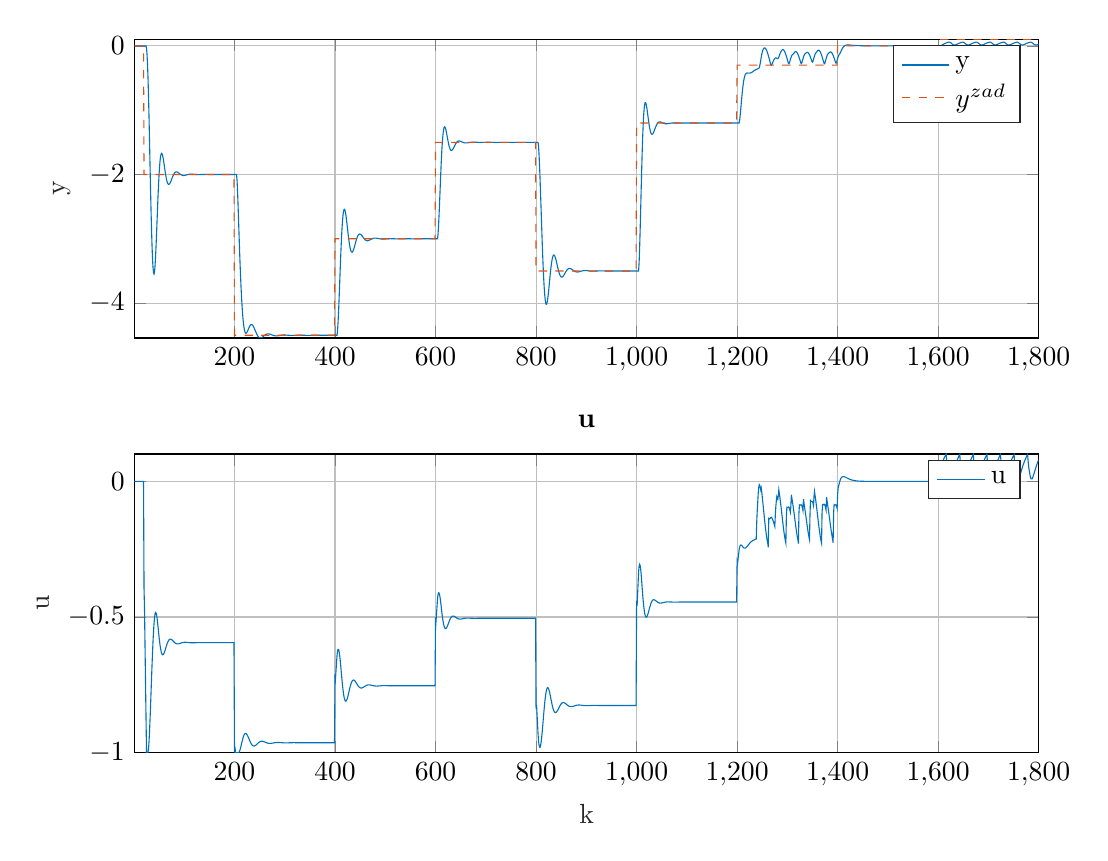
\begin{tikzpicture}

\begin{axis}[%
width=4.521in,
height=1.493in,
at={(0.758in,2.554in)},
scale only axis,
xmin=1,
xmax=1800,
ymin=-4.5419,
ymax=0.1,
ylabel style={font=\color{white!15!black}},
ylabel={y},
axis background/.style={fill=white},
xmajorgrids,
ymajorgrids,
legend style={legend cell align=left, align=left, draw=white!15!black}
]
\addplot [color=mycolor1]
  table[row sep=crcr]{%
1	0\\
2	0\\
3	0\\
4	0\\
5	0\\
6	0\\
7	0\\
8	0\\
9	0\\
10	0\\
11	0\\
12	0\\
13	0\\
14	0\\
15	0\\
16	0\\
17	0\\
18	0\\
19	0\\
20	0\\
21	0\\
22	0\\
23	0\\
24	0\\
25	-0.037705\\
26	-0.13822\\
27	-0.29676\\
28	-0.51497\\
29	-0.79316\\
30	-1.1289\\
31	-1.4987\\
32	-1.8745\\
33	-2.2376\\
34	-2.5744\\
35	-2.8732\\
36	-3.1242\\
37	-3.3203\\
38	-3.457\\
39	-3.5323\\
40	-3.547\\
41	-3.5044\\
42	-3.4103\\
43	-3.2728\\
44	-3.1018\\
45	-2.9088\\
46	-2.7054\\
47	-2.5029\\
48	-2.3114\\
49	-2.1387\\
50	-1.9907\\
51	-1.8706\\
52	-1.7797\\
53	-1.7176\\
54	-1.6824\\
55	-1.6711\\
56	-1.6804\\
57	-1.7064\\
58	-1.7452\\
59	-1.7927\\
60	-1.8454\\
61	-1.8999\\
62	-1.9534\\
63	-2.0033\\
64	-2.0477\\
65	-2.0852\\
66	-2.1148\\
67	-2.1362\\
68	-2.1493\\
69	-2.1546\\
70	-2.1527\\
71	-2.1447\\
72	-2.1316\\
73	-2.1147\\
74	-2.0953\\
75	-2.0746\\
76	-2.0538\\
77	-2.0337\\
78	-2.0152\\
79	-1.999\\
80	-1.9854\\
81	-1.9747\\
82	-1.967\\
83	-1.9621\\
84	-1.96\\
85	-1.9602\\
86	-1.9624\\
87	-1.9663\\
88	-1.9713\\
89	-1.9771\\
90	-1.9833\\
91	-1.9895\\
92	-1.9954\\
93	-2.0008\\
94	-2.0055\\
95	-2.0093\\
96	-2.0122\\
97	-2.0142\\
98	-2.0153\\
99	-2.0155\\
100	-2.0151\\
101	-2.014\\
102	-2.0124\\
103	-2.0105\\
104	-2.0084\\
105	-2.0062\\
106	-2.0041\\
107	-2.0021\\
108	-2.0003\\
109	-1.9987\\
110	-1.9974\\
111	-1.9965\\
112	-1.9959\\
113	-1.9955\\
114	-1.9954\\
115	-1.9956\\
116	-1.996\\
117	-1.9965\\
118	-1.9971\\
119	-1.9977\\
120	-1.9984\\
121	-1.9991\\
122	-1.9997\\
123	-2.0003\\
124	-2.0007\\
125	-2.0011\\
126	-2.0014\\
127	-2.0015\\
128	-2.0016\\
129	-2.0016\\
130	-2.0015\\
131	-2.0014\\
132	-2.0012\\
133	-2.001\\
134	-2.0008\\
135	-2.0005\\
136	-2.0003\\
137	-2.0001\\
138	-1.9999\\
139	-1.9998\\
140	-1.9997\\
141	-1.9996\\
142	-1.9995\\
143	-1.9995\\
144	-1.9995\\
145	-1.9995\\
146	-1.9996\\
147	-1.9996\\
148	-1.9997\\
149	-1.9998\\
150	-1.9999\\
151	-1.9999\\
152	-2\\
153	-2\\
154	-2.0001\\
155	-2.0001\\
156	-2.0002\\
157	-2.0002\\
158	-2.0002\\
159	-2.0002\\
160	-2.0002\\
161	-2.0001\\
162	-2.0001\\
163	-2.0001\\
164	-2.0001\\
165	-2\\
166	-2\\
167	-2\\
168	-2\\
169	-2\\
170	-2\\
171	-1.9999\\
172	-1.9999\\
173	-1.9999\\
174	-1.9999\\
175	-2\\
176	-2\\
177	-2\\
178	-2\\
179	-2\\
180	-2\\
181	-2\\
182	-2\\
183	-2\\
184	-2\\
185	-2\\
186	-2\\
187	-2\\
188	-2\\
189	-2\\
190	-2\\
191	-2\\
192	-2\\
193	-2\\
194	-2\\
195	-2\\
196	-2\\
197	-2\\
198	-2\\
199	-2\\
200	-2\\
201	-2\\
202	-2\\
203	-2\\
204	-2\\
205	-2.0801\\
206	-2.2427\\
207	-2.4526\\
208	-2.6856\\
209	-2.9234\\
210	-3.1541\\
211	-3.3704\\
212	-3.5682\\
213	-3.7459\\
214	-3.903\\
215	-4.0393\\
216	-4.155\\
217	-4.2505\\
218	-4.3267\\
219	-4.3847\\
220	-4.426\\
221	-4.4525\\
222	-4.4661\\
223	-4.4689\\
224	-4.4632\\
225	-4.451\\
226	-4.4346\\
227	-4.4158\\
228	-4.3963\\
229	-4.3778\\
230	-4.3614\\
231	-4.3482\\
232	-4.3387\\
233	-4.3334\\
234	-4.3325\\
235	-4.3358\\
236	-4.3431\\
237	-4.354\\
238	-4.3678\\
239	-4.3839\\
240	-4.4017\\
241	-4.4205\\
242	-4.4394\\
243	-4.458\\
244	-4.4756\\
245	-4.4917\\
246	-4.5059\\
247	-4.5179\\
248	-4.5275\\
249	-4.5347\\
250	-4.5394\\
251	-4.5418\\
252	-4.5419\\
253	-4.5402\\
254	-4.5368\\
255	-4.532\\
256	-4.5263\\
257	-4.52\\
258	-4.5133\\
259	-4.5066\\
260	-4.5002\\
261	-4.4944\\
262	-4.4892\\
263	-4.4849\\
264	-4.4816\\
265	-4.4792\\
266	-4.4779\\
267	-4.4775\\
268	-4.478\\
269	-4.4793\\
270	-4.4812\\
271	-4.4836\\
272	-4.4865\\
273	-4.4895\\
274	-4.4927\\
275	-4.4958\\
276	-4.4988\\
277	-4.5015\\
278	-4.5038\\
279	-4.5058\\
280	-4.5073\\
281	-4.5084\\
282	-4.5091\\
283	-4.5093\\
284	-4.5091\\
285	-4.5086\\
286	-4.5078\\
287	-4.5067\\
288	-4.5055\\
289	-4.5042\\
290	-4.5028\\
291	-4.5015\\
292	-4.5002\\
293	-4.4991\\
294	-4.4981\\
295	-4.4973\\
296	-4.4966\\
297	-4.4962\\
298	-4.4959\\
299	-4.4958\\
300	-4.496\\
301	-4.4962\\
302	-4.4966\\
303	-4.4971\\
304	-4.4976\\
305	-4.4982\\
306	-4.4988\\
307	-4.4994\\
308	-4.4999\\
309	-4.5004\\
310	-4.5009\\
311	-4.5012\\
312	-4.5015\\
313	-4.5017\\
314	-4.5018\\
315	-4.5018\\
316	-4.5018\\
317	-4.5016\\
318	-4.5015\\
319	-4.5013\\
320	-4.501\\
321	-4.5008\\
322	-4.5005\\
323	-4.5003\\
324	-4.5\\
325	-4.4998\\
326	-4.4996\\
327	-4.4995\\
328	-4.4993\\
329	-4.4993\\
330	-4.4992\\
331	-4.4992\\
332	-4.4992\\
333	-4.4993\\
334	-4.4994\\
335	-4.4995\\
336	-4.4996\\
337	-4.4997\\
338	-4.4998\\
339	-4.4999\\
340	-4.5\\
341	-4.5001\\
342	-4.5002\\
343	-4.5002\\
344	-4.5003\\
345	-4.5003\\
346	-4.5003\\
347	-4.5003\\
348	-4.5003\\
349	-4.5003\\
350	-4.5003\\
351	-4.5002\\
352	-4.5002\\
353	-4.5001\\
354	-4.5001\\
355	-4.5\\
356	-4.5\\
357	-4.5\\
358	-4.4999\\
359	-4.4999\\
360	-4.4999\\
361	-4.4999\\
362	-4.4998\\
363	-4.4998\\
364	-4.4999\\
365	-4.4999\\
366	-4.4999\\
367	-4.4999\\
368	-4.4999\\
369	-4.4999\\
370	-4.5\\
371	-4.5\\
372	-4.5\\
373	-4.5\\
374	-4.5\\
375	-4.5\\
376	-4.5001\\
377	-4.5001\\
378	-4.5001\\
379	-4.5001\\
380	-4.5001\\
381	-4.5001\\
382	-4.5001\\
383	-4.5\\
384	-4.5\\
385	-4.5\\
386	-4.5\\
387	-4.5\\
388	-4.5\\
389	-4.5\\
390	-4.5\\
391	-4.5\\
392	-4.5\\
393	-4.5\\
394	-4.5\\
395	-4.5\\
396	-4.5\\
397	-4.5\\
398	-4.5\\
399	-4.5\\
400	-4.5\\
401	-4.5\\
402	-4.5\\
403	-4.5\\
404	-4.5\\
405	-4.4319\\
406	-4.3057\\
407	-4.143\\
408	-3.9553\\
409	-3.7516\\
410	-3.5418\\
411	-3.3365\\
412	-3.1448\\
413	-2.9739\\
414	-2.8288\\
415	-2.7127\\
416	-2.6269\\
417	-2.5708\\
418	-2.5429\\
419	-2.5405\\
420	-2.5601\\
421	-2.598\\
422	-2.65\\
423	-2.7121\\
424	-2.7804\\
425	-2.851\\
426	-2.9208\\
427	-2.9868\\
428	-3.0467\\
429	-3.0985\\
430	-3.1409\\
431	-3.1731\\
432	-3.1949\\
433	-3.2063\\
434	-3.2081\\
435	-3.2012\\
436	-3.1867\\
437	-3.1662\\
438	-3.1412\\
439	-3.1133\\
440	-3.0839\\
441	-3.0545\\
442	-3.0265\\
443	-3.0007\\
444	-2.9781\\
445	-2.9593\\
446	-2.9446\\
447	-2.9341\\
448	-2.9279\\
449	-2.9256\\
450	-2.9268\\
451	-2.9311\\
452	-2.938\\
453	-2.9468\\
454	-2.9569\\
455	-2.9677\\
456	-2.9786\\
457	-2.9893\\
458	-2.9992\\
459	-3.008\\
460	-3.0155\\
461	-3.0215\\
462	-3.0258\\
463	-3.0286\\
464	-3.0298\\
465	-3.0297\\
466	-3.0282\\
467	-3.0258\\
468	-3.0225\\
469	-3.0187\\
470	-3.0145\\
471	-3.0102\\
472	-3.0059\\
473	-3.0019\\
474	-2.9983\\
475	-2.9952\\
476	-2.9927\\
477	-2.9908\\
478	-2.9895\\
479	-2.9888\\
480	-2.9887\\
481	-2.9891\\
482	-2.9899\\
483	-2.9911\\
484	-2.9925\\
485	-2.994\\
486	-2.9957\\
487	-2.9973\\
488	-2.9989\\
489	-3.0003\\
490	-3.0016\\
491	-3.0026\\
492	-3.0034\\
493	-3.004\\
494	-3.0043\\
495	-3.0044\\
496	-3.0043\\
497	-3.004\\
498	-3.0036\\
499	-3.0031\\
500	-3.0025\\
501	-3.0019\\
502	-3.0012\\
503	-3.0006\\
504	-3.0001\\
505	-2.9996\\
506	-2.9991\\
507	-2.9988\\
508	-2.9985\\
509	-2.9984\\
510	-2.9983\\
511	-2.9983\\
512	-2.9984\\
513	-2.9986\\
514	-2.9987\\
515	-2.999\\
516	-2.9992\\
517	-2.9994\\
518	-2.9997\\
519	-2.9999\\
520	-3.0001\\
521	-3.0003\\
522	-3.0004\\
523	-3.0005\\
524	-3.0006\\
525	-3.0006\\
526	-3.0007\\
527	-3.0006\\
528	-3.0006\\
529	-3.0005\\
530	-3.0004\\
531	-3.0003\\
532	-3.0002\\
533	-3.0001\\
534	-3.0001\\
535	-3\\
536	-2.9999\\
537	-2.9998\\
538	-2.9998\\
539	-2.9998\\
540	-2.9998\\
541	-2.9997\\
542	-2.9998\\
543	-2.9998\\
544	-2.9998\\
545	-2.9998\\
546	-2.9999\\
547	-2.9999\\
548	-2.9999\\
549	-3\\
550	-3\\
551	-3\\
552	-3.0001\\
553	-3.0001\\
554	-3.0001\\
555	-3.0001\\
556	-3.0001\\
557	-3.0001\\
558	-3.0001\\
559	-3.0001\\
560	-3.0001\\
561	-3.0001\\
562	-3\\
563	-3\\
564	-3\\
565	-3\\
566	-3\\
567	-3\\
568	-3\\
569	-3\\
570	-3\\
571	-3\\
572	-3\\
573	-3\\
574	-3\\
575	-3\\
576	-3\\
577	-3\\
578	-3\\
579	-3\\
580	-3\\
581	-3\\
582	-3\\
583	-3\\
584	-3\\
585	-3\\
586	-3\\
587	-3\\
588	-3\\
589	-3\\
590	-3\\
591	-3\\
592	-3\\
593	-3\\
594	-3\\
595	-3\\
596	-3\\
597	-3\\
598	-3\\
599	-3\\
600	-3\\
601	-3\\
602	-3\\
603	-3\\
604	-3\\
605	-2.9262\\
606	-2.7955\\
607	-2.631\\
608	-2.4459\\
609	-2.2501\\
610	-2.0544\\
611	-1.8697\\
612	-1.704\\
613	-1.5627\\
614	-1.4488\\
615	-1.363\\
616	-1.3044\\
617	-1.2709\\
618	-1.2593\\
619	-1.266\\
620	-1.2872\\
621	-1.3192\\
622	-1.3582\\
623	-1.401\\
624	-1.4446\\
625	-1.4866\\
626	-1.5249\\
627	-1.558\\
628	-1.5849\\
629	-1.6051\\
630	-1.6185\\
631	-1.6252\\
632	-1.6259\\
633	-1.6214\\
634	-1.6125\\
635	-1.6003\\
636	-1.5858\\
637	-1.5701\\
638	-1.5541\\
639	-1.5386\\
640	-1.5242\\
641	-1.5115\\
642	-1.5007\\
643	-1.4921\\
644	-1.4858\\
645	-1.4815\\
646	-1.4792\\
647	-1.4787\\
648	-1.4796\\
649	-1.4816\\
650	-1.4845\\
651	-1.488\\
652	-1.4917\\
653	-1.4954\\
654	-1.4989\\
655	-1.502\\
656	-1.5047\\
657	-1.5069\\
658	-1.5084\\
659	-1.5094\\
660	-1.5099\\
661	-1.5098\\
662	-1.5094\\
663	-1.5086\\
664	-1.5076\\
665	-1.5064\\
666	-1.5051\\
667	-1.5039\\
668	-1.5026\\
669	-1.5015\\
670	-1.5005\\
671	-1.4997\\
672	-1.4991\\
673	-1.4986\\
674	-1.4983\\
675	-1.4982\\
676	-1.4982\\
677	-1.4983\\
678	-1.4985\\
679	-1.4987\\
680	-1.499\\
681	-1.4993\\
682	-1.4996\\
683	-1.4999\\
684	-1.5002\\
685	-1.5004\\
686	-1.5006\\
687	-1.5007\\
688	-1.5007\\
689	-1.5008\\
690	-1.5008\\
691	-1.5007\\
692	-1.5007\\
693	-1.5006\\
694	-1.5005\\
695	-1.5004\\
696	-1.5003\\
697	-1.5002\\
698	-1.5001\\
699	-1.5\\
700	-1.5\\
701	-1.4999\\
702	-1.4999\\
703	-1.4999\\
704	-1.4998\\
705	-1.4998\\
706	-1.4999\\
707	-1.4999\\
708	-1.4999\\
709	-1.4999\\
710	-1.4999\\
711	-1.5\\
712	-1.5\\
713	-1.5\\
714	-1.5\\
715	-1.5\\
716	-1.5001\\
717	-1.5001\\
718	-1.5001\\
719	-1.5001\\
720	-1.5001\\
721	-1.5001\\
722	-1.5\\
723	-1.5\\
724	-1.5\\
725	-1.5\\
726	-1.5\\
727	-1.5\\
728	-1.5\\
729	-1.5\\
730	-1.5\\
731	-1.5\\
732	-1.5\\
733	-1.5\\
734	-1.5\\
735	-1.5\\
736	-1.5\\
737	-1.5\\
738	-1.5\\
739	-1.5\\
740	-1.5\\
741	-1.5\\
742	-1.5\\
743	-1.5\\
744	-1.5\\
745	-1.5\\
746	-1.5\\
747	-1.5\\
748	-1.5\\
749	-1.5\\
750	-1.5\\
751	-1.5\\
752	-1.5\\
753	-1.5\\
754	-1.5\\
755	-1.5\\
756	-1.5\\
757	-1.5\\
758	-1.5\\
759	-1.5\\
760	-1.5\\
761	-1.5\\
762	-1.5\\
763	-1.5\\
764	-1.5\\
765	-1.5\\
766	-1.5\\
767	-1.5\\
768	-1.5\\
769	-1.5\\
770	-1.5\\
771	-1.5\\
772	-1.5\\
773	-1.5\\
774	-1.5\\
775	-1.5\\
776	-1.5\\
777	-1.5\\
778	-1.5\\
779	-1.5\\
780	-1.5\\
781	-1.5\\
782	-1.5\\
783	-1.5\\
784	-1.5\\
785	-1.5\\
786	-1.5\\
787	-1.5\\
788	-1.5\\
789	-1.5\\
790	-1.5\\
791	-1.5\\
792	-1.5\\
793	-1.5\\
794	-1.5\\
795	-1.5\\
796	-1.5\\
797	-1.5\\
798	-1.5\\
799	-1.5\\
800	-1.5\\
801	-1.5\\
802	-1.5\\
803	-1.5\\
804	-1.5\\
805	-1.567\\
806	-1.7013\\
807	-1.877\\
808	-2.0809\\
809	-2.3039\\
810	-2.5375\\
811	-2.7728\\
812	-3.0019\\
813	-3.2178\\
814	-3.4145\\
815	-3.5876\\
816	-3.7335\\
817	-3.8499\\
818	-3.9358\\
819	-3.9911\\
820	-4.0172\\
821	-4.0161\\
822	-3.9909\\
823	-3.9454\\
824	-3.8839\\
825	-3.8108\\
826	-3.7307\\
827	-3.6481\\
828	-3.5669\\
829	-3.4908\\
830	-3.4227\\
831	-3.3645\\
832	-3.3179\\
833	-3.2836\\
834	-3.2617\\
835	-3.2518\\
836	-3.2529\\
837	-3.2638\\
838	-3.283\\
839	-3.3087\\
840	-3.3393\\
841	-3.3729\\
842	-3.4078\\
843	-3.4426\\
844	-3.4758\\
845	-3.5062\\
846	-3.533\\
847	-3.5554\\
848	-3.573\\
849	-3.5856\\
850	-3.5932\\
851	-3.596\\
852	-3.5945\\
853	-3.5892\\
854	-3.5807\\
855	-3.5697\\
856	-3.5569\\
857	-3.5432\\
858	-3.5291\\
859	-3.5153\\
860	-3.5024\\
861	-3.4908\\
862	-3.4808\\
863	-3.4727\\
864	-3.4666\\
865	-3.4626\\
866	-3.4605\\
867	-3.4604\\
868	-3.4619\\
869	-3.4648\\
870	-3.4688\\
871	-3.4737\\
872	-3.4792\\
873	-3.4849\\
874	-3.4906\\
875	-3.4961\\
876	-3.5011\\
877	-3.5056\\
878	-3.5093\\
879	-3.5122\\
880	-3.5143\\
881	-3.5156\\
882	-3.5161\\
883	-3.5159\\
884	-3.515\\
885	-3.5136\\
886	-3.5118\\
887	-3.5096\\
888	-3.5074\\
889	-3.505\\
890	-3.5027\\
891	-3.5006\\
892	-3.4986\\
893	-3.497\\
894	-3.4956\\
895	-3.4946\\
896	-3.4939\\
897	-3.4935\\
898	-3.4935\\
899	-3.4937\\
900	-3.4941\\
901	-3.4948\\
902	-3.4956\\
903	-3.4965\\
904	-3.4974\\
905	-3.4984\\
906	-3.4993\\
907	-3.5001\\
908	-3.5009\\
909	-3.5015\\
910	-3.502\\
911	-3.5024\\
912	-3.5026\\
913	-3.5027\\
914	-3.5026\\
915	-3.5025\\
916	-3.5023\\
917	-3.502\\
918	-3.5016\\
919	-3.5012\\
920	-3.5009\\
921	-3.5005\\
922	-3.5001\\
923	-3.4998\\
924	-3.4995\\
925	-3.4993\\
926	-3.4991\\
927	-3.499\\
928	-3.4989\\
929	-3.4989\\
930	-3.4989\\
931	-3.499\\
932	-3.4991\\
933	-3.4993\\
934	-3.4994\\
935	-3.4996\\
936	-3.4997\\
937	-3.4999\\
938	-3.5\\
939	-3.5001\\
940	-3.5002\\
941	-3.5003\\
942	-3.5004\\
943	-3.5004\\
944	-3.5004\\
945	-3.5004\\
946	-3.5004\\
947	-3.5004\\
948	-3.5003\\
949	-3.5003\\
950	-3.5002\\
951	-3.5001\\
952	-3.5001\\
953	-3.5\\
954	-3.5\\
955	-3.4999\\
956	-3.4999\\
957	-3.4999\\
958	-3.4998\\
959	-3.4998\\
960	-3.4998\\
961	-3.4998\\
962	-3.4998\\
963	-3.4999\\
964	-3.4999\\
965	-3.4999\\
966	-3.4999\\
967	-3.5\\
968	-3.5\\
969	-3.5\\
970	-3.5\\
971	-3.5\\
972	-3.5001\\
973	-3.5001\\
974	-3.5001\\
975	-3.5001\\
976	-3.5001\\
977	-3.5001\\
978	-3.5001\\
979	-3.5001\\
980	-3.5\\
981	-3.5\\
982	-3.5\\
983	-3.5\\
984	-3.5\\
985	-3.5\\
986	-3.5\\
987	-3.5\\
988	-3.5\\
989	-3.5\\
990	-3.5\\
991	-3.5\\
992	-3.5\\
993	-3.5\\
994	-3.5\\
995	-3.5\\
996	-3.5\\
997	-3.5\\
998	-3.5\\
999	-3.5\\
1000	-3.5\\
1001	-3.5\\
1002	-3.5\\
1003	-3.5\\
1004	-3.5\\
1005	-3.3746\\
1006	-3.1592\\
1007	-2.8907\\
1008	-2.5911\\
1009	-2.2772\\
1010	-1.9699\\
1011	-1.6876\\
1012	-1.4432\\
1013	-1.2434\\
1014	-1.0904\\
1015	-0.98243\\
1016	-0.91576\\
1017	-0.88498\\
1018	-0.88403\\
1019	-0.90662\\
1020	-0.94665\\
1021	-0.9984\\
1022	-1.0567\\
1023	-1.1171\\
1024	-1.1757\\
1025	-1.2296\\
1026	-1.2766\\
1027	-1.315\\
1028	-1.344\\
1029	-1.3635\\
1030	-1.3737\\
1031	-1.3755\\
1032	-1.3699\\
1033	-1.3582\\
1034	-1.3421\\
1035	-1.3229\\
1036	-1.3021\\
1037	-1.2809\\
1038	-1.2605\\
1039	-1.2416\\
1040	-1.225\\
1041	-1.211\\
1042	-1.1999\\
1043	-1.1916\\
1044	-1.1861\\
1045	-1.183\\
1046	-1.182\\
1047	-1.1828\\
1048	-1.1849\\
1049	-1.1879\\
1050	-1.1915\\
1051	-1.1954\\
1052	-1.1992\\
1053	-1.2028\\
1054	-1.2059\\
1055	-1.2084\\
1056	-1.2103\\
1057	-1.2116\\
1058	-1.2123\\
1059	-1.2124\\
1060	-1.212\\
1061	-1.2112\\
1062	-1.2102\\
1063	-1.2089\\
1064	-1.2075\\
1065	-1.2061\\
1066	-1.2047\\
1067	-1.2035\\
1068	-1.2023\\
1069	-1.2014\\
1070	-1.2006\\
1071	-1.2\\
1072	-1.1996\\
1073	-1.1993\\
1074	-1.1992\\
1075	-1.1992\\
1076	-1.1993\\
1077	-1.1994\\
1078	-1.1996\\
1079	-1.1999\\
1080	-1.2001\\
1081	-1.2003\\
1082	-1.2005\\
1083	-1.2006\\
1084	-1.2008\\
1085	-1.2008\\
1086	-1.2009\\
1087	-1.2009\\
1088	-1.2009\\
1089	-1.2008\\
1090	-1.2007\\
1091	-1.2007\\
1092	-1.2006\\
1093	-1.2005\\
1094	-1.2004\\
1095	-1.2003\\
1096	-1.2002\\
1097	-1.2001\\
1098	-1.2001\\
1099	-1.2\\
1100	-1.2\\
1101	-1.2\\
1102	-1.2\\
1103	-1.2\\
1104	-1.2\\
1105	-1.2\\
1106	-1.2\\
1107	-1.2\\
1108	-1.2\\
1109	-1.2\\
1110	-1.2\\
1111	-1.2001\\
1112	-1.2001\\
1113	-1.2001\\
1114	-1.2001\\
1115	-1.2001\\
1116	-1.2001\\
1117	-1.2001\\
1118	-1.2001\\
1119	-1.2\\
1120	-1.2\\
1121	-1.2\\
1122	-1.2\\
1123	-1.2\\
1124	-1.2\\
1125	-1.2\\
1126	-1.2\\
1127	-1.2\\
1128	-1.2\\
1129	-1.2\\
1130	-1.2\\
1131	-1.2\\
1132	-1.2\\
1133	-1.2\\
1134	-1.2\\
1135	-1.2\\
1136	-1.2\\
1137	-1.2\\
1138	-1.2\\
1139	-1.2\\
1140	-1.2\\
1141	-1.2\\
1142	-1.2\\
1143	-1.2\\
1144	-1.2\\
1145	-1.2\\
1146	-1.2\\
1147	-1.2\\
1148	-1.2\\
1149	-1.2\\
1150	-1.2\\
1151	-1.2\\
1152	-1.2\\
1153	-1.2\\
1154	-1.2\\
1155	-1.2\\
1156	-1.2\\
1157	-1.2\\
1158	-1.2\\
1159	-1.2\\
1160	-1.2\\
1161	-1.2\\
1162	-1.2\\
1163	-1.2\\
1164	-1.2\\
1165	-1.2\\
1166	-1.2\\
1167	-1.2\\
1168	-1.2\\
1169	-1.2\\
1170	-1.2\\
1171	-1.2\\
1172	-1.2\\
1173	-1.2\\
1174	-1.2\\
1175	-1.2\\
1176	-1.2\\
1177	-1.2\\
1178	-1.2\\
1179	-1.2\\
1180	-1.2\\
1181	-1.2\\
1182	-1.2\\
1183	-1.2\\
1184	-1.2\\
1185	-1.2\\
1186	-1.2\\
1187	-1.2\\
1188	-1.2\\
1189	-1.2\\
1190	-1.2\\
1191	-1.2\\
1192	-1.2\\
1193	-1.2\\
1194	-1.2\\
1195	-1.2\\
1196	-1.2\\
1197	-1.2\\
1198	-1.2\\
1199	-1.2\\
1200	-1.2\\
1201	-1.2\\
1202	-1.2\\
1203	-1.2\\
1204	-1.2\\
1205	-1.1595\\
1206	-1.0904\\
1207	-1.0075\\
1208	-0.91874\\
1209	-0.82958\\
1210	-0.7449\\
1211	-0.66863\\
1212	-0.60311\\
1213	-0.54926\\
1214	-0.50692\\
1215	-0.4752\\
1216	-0.45274\\
1217	-0.43794\\
1218	-0.42911\\
1219	-0.42465\\
1220	-0.42312\\
1221	-0.42329\\
1222	-0.42418\\
1223	-0.42504\\
1224	-0.42536\\
1225	-0.42481\\
1226	-0.42326\\
1227	-0.4207\\
1228	-0.41721\\
1229	-0.41295\\
1230	-0.40811\\
1231	-0.40289\\
1232	-0.39746\\
1233	-0.392\\
1234	-0.38665\\
1235	-0.38152\\
1236	-0.37667\\
1237	-0.37216\\
1238	-0.36799\\
1239	-0.36418\\
1240	-0.3607\\
1241	-0.35754\\
1242	-0.35465\\
1243	-0.352\\
1244	-0.33925\\
1245	-0.31168\\
1246	-0.27279\\
1247	-0.22691\\
1248	-0.17963\\
1249	-0.13595\\
1250	-0.099474\\
1251	-0.071889\\
1252	-0.053136\\
1253	-0.040906\\
1254	-0.034055\\
1255	-0.032874\\
1256	-0.037108\\
1257	-0.04626\\
1258	-0.05979\\
1259	-0.07719\\
1260	-0.097977\\
1261	-0.12166\\
1262	-0.14772\\
1263	-0.17559\\
1264	-0.20468\\
1265	-0.23431\\
1266	-0.26378\\
1267	-0.29346\\
1268	-0.30264\\
1269	-0.29368\\
1270	-0.27665\\
1271	-0.25719\\
1272	-0.23808\\
1273	-0.22095\\
1274	-0.20697\\
1275	-0.19672\\
1276	-0.19034\\
1277	-0.18767\\
1278	-0.18837\\
1279	-0.19202\\
1280	-0.19814\\
1281	-0.19925\\
1282	-0.19086\\
1283	-0.17418\\
1284	-0.15242\\
1285	-0.13053\\
1286	-0.11213\\
1287	-0.096708\\
1288	-0.081911\\
1289	-0.069305\\
1290	-0.061343\\
1291	-0.058714\\
1292	-0.061303\\
1293	-0.06872\\
1294	-0.080516\\
1295	-0.096216\\
1296	-0.11532\\
1297	-0.1373\\
1298	-0.16162\\
1299	-0.18769\\
1300	-0.21488\\
1301	-0.24254\\
1302	-0.26998\\
1303	-0.27847\\
1304	-0.26473\\
1305	-0.23984\\
1306	-0.21251\\
1307	-0.18699\\
1308	-0.16536\\
1309	-0.1487\\
1310	-0.13745\\
1311	-0.13149\\
1312	-0.12636\\
1313	-0.11635\\
1314	-0.10441\\
1315	-0.095081\\
1316	-0.09009\\
1317	-0.089818\\
1318	-0.094143\\
1319	-0.10278\\
1320	-0.11535\\
1321	-0.13137\\
1322	-0.15033\\
1323	-0.17169\\
1324	-0.19486\\
1325	-0.21923\\
1326	-0.24419\\
1327	-0.27007\\
1328	-0.27573\\
1329	-0.25877\\
1330	-0.23122\\
1331	-0.20195\\
1332	-0.17518\\
1333	-0.15287\\
1334	-0.13602\\
1335	-0.12494\\
1336	-0.11941\\
1337	-0.11298\\
1338	-0.10588\\
1339	-0.10155\\
1340	-0.10128\\
1341	-0.10528\\
1342	-0.11334\\
1343	-0.12512\\
1344	-0.14023\\
1345	-0.15819\\
1346	-0.17847\\
1347	-0.20051\\
1348	-0.22371\\
1349	-0.24747\\
1350	-0.25467\\
1351	-0.23902\\
1352	-0.21159\\
1353	-0.18223\\
1354	-0.15562\\
1355	-0.1338\\
1356	-0.11766\\
1357	-0.10743\\
1358	-0.098182\\
1359	-0.086802\\
1360	-0.076108\\
1361	-0.069165\\
1362	-0.067021\\
1363	-0.069745\\
1364	-0.077073\\
1365	-0.088639\\
1366	-0.10401\\
1367	-0.12271\\
1368	-0.14422\\
1369	-0.16799\\
1370	-0.19343\\
1371	-0.21994\\
1372	-0.24684\\
1373	-0.27346\\
1374	-0.27879\\
1375	-0.26109\\
1376	-0.23268\\
1377	-0.20256\\
1378	-0.17499\\
1379	-0.15199\\
1380	-0.13459\\
1381	-0.12308\\
1382	-0.11724\\
1383	-0.11005\\
1384	-0.10175\\
1385	-0.096136\\
1386	-0.094675\\
1387	-0.097638\\
1388	-0.10483\\
1389	-0.11593\\
1390	-0.13054\\
1391	-0.1482\\
1392	-0.16838\\
1393	-0.19052\\
1394	-0.21403\\
1395	-0.2383\\
1396	-0.26367\\
1397	-0.26941\\
1398	-0.25306\\
1399	-0.22642\\
1400	-0.19815\\
1401	-0.17238\\
1402	-0.151\\
1403	-0.13498\\
1404	-0.1246\\
1405	-0.11289\\
1406	-0.096778\\
1407	-0.078866\\
1408	-0.061567\\
1409	-0.045959\\
1410	-0.032434\\
1411	-0.02108\\
1412	-0.011822\\
1413	-0.0044753\\
1414	0.0012044\\
1415	0.0054747\\
1416	0.0085819\\
1417	0.010748\\
1418	0.012166\\
1419	0.012999\\
1420	0.013381\\
1421	0.013422\\
1422	0.013208\\
1423	0.01281\\
1424	0.012283\\
1425	0.011669\\
1426	0.011001\\
1427	0.010304\\
1428	0.0095987\\
1429	0.0088984\\
1430	0.0082141\\
1431	0.0075536\\
1432	0.0069221\\
1433	0.0063234\\
1434	0.0057596\\
1435	0.0052318\\
1436	0.0047402\\
1437	0.0042844\\
1438	0.0038636\\
1439	0.0034765\\
1440	0.0031217\\
1441	0.0027975\\
1442	0.0025021\\
1443	0.0022337\\
1444	0.0019905\\
1445	0.0017707\\
1446	0.0015725\\
1447	0.0013942\\
1448	0.0012341\\
1449	0.0010907\\
1450	0.00096245\\
1451	0.00084802\\
1452	0.00074609\\
1453	0.00065547\\
1454	0.00057504\\
1455	0.00050377\\
1456	0.00044073\\
1457	0.00038505\\
1458	0.00033596\\
1459	0.00029273\\
1460	0.00025474\\
1461	0.00022138\\
1462	0.00019214\\
1463	0.00016655\\
1464	0.00014418\\
1465	0.00012465\\
1466	0.00010763\\
1467	9.2807e-05\\
1468	7.9923e-05\\
1469	6.8736e-05\\
1470	5.9037e-05\\
1471	5.0637e-05\\
1472	4.3372e-05\\
1473	3.7097e-05\\
1474	3.1685e-05\\
1475	2.7023e-05\\
1476	2.3012e-05\\
1477	1.9565e-05\\
1478	1.6609e-05\\
1479	1.4076e-05\\
1480	1.1908e-05\\
1481	1.0056e-05\\
1482	8.4765e-06\\
1483	7.1308e-06\\
1484	5.9863e-06\\
1485	5.0144e-06\\
1486	4.1904e-06\\
1487	3.4931e-06\\
1488	2.904e-06\\
1489	2.4072e-06\\
1490	1.9891e-06\\
1491	1.638e-06\\
1492	1.3438e-06\\
1493	1.0978e-06\\
1494	8.9264e-07\\
1495	7.2198e-07\\
1496	5.8043e-07\\
1497	4.6339e-07\\
1498	3.6694e-07\\
1499	2.8775e-07\\
1500	2.23e-07\\
1501	1.703e-07\\
1502	1.2763e-07\\
1503	9.3286e-08\\
1504	6.5825e-08\\
1505	4.4042e-08\\
1506	2.6925e-08\\
1507	1.3626e-08\\
1508	3.4374e-09\\
1509	-4.2299e-09\\
1510	-9.8651e-09\\
1511	-1.3873e-08\\
1512	-1.6589e-08\\
1513	-1.8287e-08\\
1514	-1.9192e-08\\
1515	-1.9488e-08\\
1516	-1.9324e-08\\
1517	-1.882e-08\\
1518	-1.8073e-08\\
1519	-1.7158e-08\\
1520	-1.6137e-08\\
1521	-1.5057e-08\\
1522	-1.3953e-08\\
1523	-1.2855e-08\\
1524	-1.1782e-08\\
1525	-1.0749e-08\\
1526	-9.7657e-09\\
1527	-8.8397e-09\\
1528	-7.9744e-09\\
1529	-7.1715e-09\\
1530	-6.431e-09\\
1531	-5.7517e-09\\
1532	-5.1314e-09\\
1533	-4.5674e-09\\
1534	-4.0565e-09\\
1535	-3.5953e-09\\
1536	-3.1803e-09\\
1537	-2.8079e-09\\
1538	-2.4747e-09\\
1539	-2.1773e-09\\
1540	-1.9125e-09\\
1541	-1.6772e-09\\
1542	-1.4686e-09\\
1543	-1.284e-09\\
1544	-1.1209e-09\\
1545	-9.7715e-10\\
1546	-8.5062e-10\\
1547	-7.3944e-10\\
1548	-6.4191e-10\\
1549	-5.5649e-10\\
1550	-4.8179e-10\\
1551	-4.1655e-10\\
1552	-3.5966e-10\\
1553	-3.1013e-10\\
1554	-2.6706e-10\\
1555	-2.2966e-10\\
1556	-1.9723e-10\\
1557	-1.6914e-10\\
1558	-1.4485e-10\\
1559	-1.2387e-10\\
1560	-1.0578e-10\\
1561	-9.0197e-11\\
1562	-7.6791e-11\\
1563	-6.5275e-11\\
1564	-5.5397e-11\\
1565	-4.6935e-11\\
1566	-3.9696e-11\\
1567	-3.3513e-11\\
1568	-2.8239e-11\\
1569	-2.3747e-11\\
1570	-1.9928e-11\\
1571	-1.6686e-11\\
1572	-1.3938e-11\\
1573	-1.1614e-11\\
1574	-9.6502e-12\\
1575	-7.9951e-12\\
1576	-6.6027e-12\\
1577	-5.4338e-12\\
1578	-4.4546e-12\\
1579	-3.6362e-12\\
1580	-2.954e-12\\
1581	-2.3868e-12\\
1582	-1.9167e-12\\
1583	-1.5281e-12\\
1584	-1.2081e-12\\
1585	-9.4556e-13\\
1586	-7.3106e-13\\
1587	-5.5663e-13\\
1588	-4.1554e-13\\
1589	-3.0209e-13\\
1590	-2.1151e-13\\
1591	-1.3976e-13\\
1592	-8.3494e-14\\
1593	-3.9874e-14\\
1594	-6.5513e-15\\
1595	1.8433e-14\\
1596	3.6703e-14\\
1597	4.9606e-14\\
1598	5.825e-14\\
1599	6.3547e-14\\
1600	6.6242e-14\\
1601	6.6945e-14\\
1602	6.6146e-14\\
1603	6.4244e-14\\
1604	6.1557e-14\\
1605	0.0012443\\
1606	0.0041234\\
1607	0.0078733\\
1608	0.012148\\
1609	0.01669\\
1610	0.021308\\
1611	0.025852\\
1612	0.030213\\
1613	0.034325\\
1614	0.038151\\
1615	0.041676\\
1616	0.044905\\
1617	0.047849\\
1618	0.050529\\
1619	0.052967\\
1620	0.055189\\
1621	0.057217\\
1622	0.05831\\
1623	0.057008\\
1624	0.053454\\
1625	0.048012\\
1626	0.041143\\
1627	0.033819\\
1628	0.026886\\
1629	0.020983\\
1630	0.016438\\
1631	0.013456\\
1632	0.01214\\
1633	0.012331\\
1634	0.013762\\
1635	0.016136\\
1636	0.019172\\
1637	0.022627\\
1638	0.026298\\
1639	0.030029\\
1640	0.033704\\
1641	0.037243\\
1642	0.040594\\
1643	0.043731\\
1644	0.046643\\
1645	0.049331\\
1646	0.051803\\
1647	0.054074\\
1648	0.056159\\
1649	0.057309\\
1650	0.056086\\
1651	0.052632\\
1652	0.047647\\
1653	0.04161\\
1654	0.034922\\
1655	0.028308\\
1656	0.022471\\
1657	0.017836\\
1658	0.014684\\
1659	0.01317\\
1660	0.013165\\
1661	0.014415\\
1662	0.01663\\
1663	0.019534\\
1664	0.022881\\
1665	0.026468\\
1666	0.030133\\
1667	0.033758\\
1668	0.037261\\
1669	0.040587\\
1670	0.043707\\
1671	0.046608\\
1672	0.049289\\
1673	0.051758\\
1674	0.054028\\
1675	0.056113\\
1676	0.057264\\
1677	0.056043\\
1678	0.052594\\
1679	0.047614\\
1680	0.041582\\
1681	0.0349\\
1682	0.028292\\
1683	0.022459\\
1684	0.017829\\
1685	0.01468\\
1686	0.013168\\
1687	0.013165\\
1688	0.014416\\
1689	0.016633\\
1690	0.019537\\
1691	0.022884\\
1692	0.026471\\
1693	0.030136\\
1694	0.033762\\
1695	0.037264\\
1696	0.04059\\
1697	0.04371\\
1698	0.046611\\
1699	0.049292\\
1700	0.05176\\
1701	0.05403\\
1702	0.056115\\
1703	0.057266\\
1704	0.056045\\
1705	0.052595\\
1706	0.047615\\
1707	0.041583\\
1708	0.034901\\
1709	0.028292\\
1710	0.02246\\
1711	0.017829\\
1712	0.01468\\
1713	0.013168\\
1714	0.013165\\
1715	0.014416\\
1716	0.016633\\
1717	0.019537\\
1718	0.022884\\
1719	0.026471\\
1720	0.030136\\
1721	0.033762\\
1722	0.037264\\
1723	0.04059\\
1724	0.04371\\
1725	0.046611\\
1726	0.049291\\
1727	0.05176\\
1728	0.054029\\
1729	0.056115\\
1730	0.057266\\
1731	0.056044\\
1732	0.052595\\
1733	0.047615\\
1734	0.041583\\
1735	0.034901\\
1736	0.028292\\
1737	0.02246\\
1738	0.017829\\
1739	0.01468\\
1740	0.013168\\
1741	0.013165\\
1742	0.014416\\
1743	0.016633\\
1744	0.019537\\
1745	0.022884\\
1746	0.026471\\
1747	0.030136\\
1748	0.033762\\
1749	0.037264\\
1750	0.04059\\
1751	0.04371\\
1752	0.046611\\
1753	0.049291\\
1754	0.05176\\
1755	0.054029\\
1756	0.056115\\
1757	0.057266\\
1758	0.056044\\
1759	0.052595\\
1760	0.047615\\
1761	0.041583\\
1762	0.034901\\
1763	0.028292\\
1764	0.02246\\
1765	0.017829\\
1766	0.01468\\
1767	0.013168\\
1768	0.013165\\
1769	0.014416\\
1770	0.016633\\
1771	0.019537\\
1772	0.022884\\
1773	0.026471\\
1774	0.030136\\
1775	0.033762\\
1776	0.037264\\
1777	0.04059\\
1778	0.04371\\
1779	0.046611\\
1780	0.049291\\
1781	0.05176\\
1782	0.054029\\
1783	0.056115\\
1784	0.057266\\
1785	0.056044\\
1786	0.052595\\
1787	0.047615\\
1788	0.041583\\
1789	0.034901\\
1790	0.028292\\
1791	0.02246\\
1792	0.017829\\
1793	0.01468\\
1794	0.013168\\
1795	0.013165\\
1796	0.014416\\
1797	0.016633\\
1798	0.019537\\
1799	0.022884\\
1800	0.026471\\
};
\addlegendentry{y}

\addplot [color=mycolor2, dashed]
  table[row sep=crcr]{%
1	0\\
2	0\\
3	0\\
4	0\\
5	0\\
6	0\\
7	0\\
8	0\\
9	0\\
10	0\\
11	0\\
12	0\\
13	0\\
14	0\\
15	0\\
16	0\\
17	0\\
18	0\\
19	0\\
20	-2\\
21	-2\\
22	-2\\
23	-2\\
24	-2\\
25	-2\\
26	-2\\
27	-2\\
28	-2\\
29	-2\\
30	-2\\
31	-2\\
32	-2\\
33	-2\\
34	-2\\
35	-2\\
36	-2\\
37	-2\\
38	-2\\
39	-2\\
40	-2\\
41	-2\\
42	-2\\
43	-2\\
44	-2\\
45	-2\\
46	-2\\
47	-2\\
48	-2\\
49	-2\\
50	-2\\
51	-2\\
52	-2\\
53	-2\\
54	-2\\
55	-2\\
56	-2\\
57	-2\\
58	-2\\
59	-2\\
60	-2\\
61	-2\\
62	-2\\
63	-2\\
64	-2\\
65	-2\\
66	-2\\
67	-2\\
68	-2\\
69	-2\\
70	-2\\
71	-2\\
72	-2\\
73	-2\\
74	-2\\
75	-2\\
76	-2\\
77	-2\\
78	-2\\
79	-2\\
80	-2\\
81	-2\\
82	-2\\
83	-2\\
84	-2\\
85	-2\\
86	-2\\
87	-2\\
88	-2\\
89	-2\\
90	-2\\
91	-2\\
92	-2\\
93	-2\\
94	-2\\
95	-2\\
96	-2\\
97	-2\\
98	-2\\
99	-2\\
100	-2\\
101	-2\\
102	-2\\
103	-2\\
104	-2\\
105	-2\\
106	-2\\
107	-2\\
108	-2\\
109	-2\\
110	-2\\
111	-2\\
112	-2\\
113	-2\\
114	-2\\
115	-2\\
116	-2\\
117	-2\\
118	-2\\
119	-2\\
120	-2\\
121	-2\\
122	-2\\
123	-2\\
124	-2\\
125	-2\\
126	-2\\
127	-2\\
128	-2\\
129	-2\\
130	-2\\
131	-2\\
132	-2\\
133	-2\\
134	-2\\
135	-2\\
136	-2\\
137	-2\\
138	-2\\
139	-2\\
140	-2\\
141	-2\\
142	-2\\
143	-2\\
144	-2\\
145	-2\\
146	-2\\
147	-2\\
148	-2\\
149	-2\\
150	-2\\
151	-2\\
152	-2\\
153	-2\\
154	-2\\
155	-2\\
156	-2\\
157	-2\\
158	-2\\
159	-2\\
160	-2\\
161	-2\\
162	-2\\
163	-2\\
164	-2\\
165	-2\\
166	-2\\
167	-2\\
168	-2\\
169	-2\\
170	-2\\
171	-2\\
172	-2\\
173	-2\\
174	-2\\
175	-2\\
176	-2\\
177	-2\\
178	-2\\
179	-2\\
180	-2\\
181	-2\\
182	-2\\
183	-2\\
184	-2\\
185	-2\\
186	-2\\
187	-2\\
188	-2\\
189	-2\\
190	-2\\
191	-2\\
192	-2\\
193	-2\\
194	-2\\
195	-2\\
196	-2\\
197	-2\\
198	-2\\
199	-2\\
200	-4.5\\
201	-4.5\\
202	-4.5\\
203	-4.5\\
204	-4.5\\
205	-4.5\\
206	-4.5\\
207	-4.5\\
208	-4.5\\
209	-4.5\\
210	-4.5\\
211	-4.5\\
212	-4.5\\
213	-4.5\\
214	-4.5\\
215	-4.5\\
216	-4.5\\
217	-4.5\\
218	-4.5\\
219	-4.5\\
220	-4.5\\
221	-4.5\\
222	-4.5\\
223	-4.5\\
224	-4.5\\
225	-4.5\\
226	-4.5\\
227	-4.5\\
228	-4.5\\
229	-4.5\\
230	-4.5\\
231	-4.5\\
232	-4.5\\
233	-4.5\\
234	-4.5\\
235	-4.5\\
236	-4.5\\
237	-4.5\\
238	-4.5\\
239	-4.5\\
240	-4.5\\
241	-4.5\\
242	-4.5\\
243	-4.5\\
244	-4.5\\
245	-4.5\\
246	-4.5\\
247	-4.5\\
248	-4.5\\
249	-4.5\\
250	-4.5\\
251	-4.5\\
252	-4.5\\
253	-4.5\\
254	-4.5\\
255	-4.5\\
256	-4.5\\
257	-4.5\\
258	-4.5\\
259	-4.5\\
260	-4.5\\
261	-4.5\\
262	-4.5\\
263	-4.5\\
264	-4.5\\
265	-4.5\\
266	-4.5\\
267	-4.5\\
268	-4.5\\
269	-4.5\\
270	-4.5\\
271	-4.5\\
272	-4.5\\
273	-4.5\\
274	-4.5\\
275	-4.5\\
276	-4.5\\
277	-4.5\\
278	-4.5\\
279	-4.5\\
280	-4.5\\
281	-4.5\\
282	-4.5\\
283	-4.5\\
284	-4.5\\
285	-4.5\\
286	-4.5\\
287	-4.5\\
288	-4.5\\
289	-4.5\\
290	-4.5\\
291	-4.5\\
292	-4.5\\
293	-4.5\\
294	-4.5\\
295	-4.5\\
296	-4.5\\
297	-4.5\\
298	-4.5\\
299	-4.5\\
300	-4.5\\
301	-4.5\\
302	-4.5\\
303	-4.5\\
304	-4.5\\
305	-4.5\\
306	-4.5\\
307	-4.5\\
308	-4.5\\
309	-4.5\\
310	-4.5\\
311	-4.5\\
312	-4.5\\
313	-4.5\\
314	-4.5\\
315	-4.5\\
316	-4.5\\
317	-4.5\\
318	-4.5\\
319	-4.5\\
320	-4.5\\
321	-4.5\\
322	-4.5\\
323	-4.5\\
324	-4.5\\
325	-4.5\\
326	-4.5\\
327	-4.5\\
328	-4.5\\
329	-4.5\\
330	-4.5\\
331	-4.5\\
332	-4.5\\
333	-4.5\\
334	-4.5\\
335	-4.5\\
336	-4.5\\
337	-4.5\\
338	-4.5\\
339	-4.5\\
340	-4.5\\
341	-4.5\\
342	-4.5\\
343	-4.5\\
344	-4.5\\
345	-4.5\\
346	-4.5\\
347	-4.5\\
348	-4.5\\
349	-4.5\\
350	-4.5\\
351	-4.5\\
352	-4.5\\
353	-4.5\\
354	-4.5\\
355	-4.5\\
356	-4.5\\
357	-4.5\\
358	-4.5\\
359	-4.5\\
360	-4.5\\
361	-4.5\\
362	-4.5\\
363	-4.5\\
364	-4.5\\
365	-4.5\\
366	-4.5\\
367	-4.5\\
368	-4.5\\
369	-4.5\\
370	-4.5\\
371	-4.5\\
372	-4.5\\
373	-4.5\\
374	-4.5\\
375	-4.5\\
376	-4.5\\
377	-4.5\\
378	-4.5\\
379	-4.5\\
380	-4.5\\
381	-4.5\\
382	-4.5\\
383	-4.5\\
384	-4.5\\
385	-4.5\\
386	-4.5\\
387	-4.5\\
388	-4.5\\
389	-4.5\\
390	-4.5\\
391	-4.5\\
392	-4.5\\
393	-4.5\\
394	-4.5\\
395	-4.5\\
396	-4.5\\
397	-4.5\\
398	-4.5\\
399	-4.5\\
400	-3\\
401	-3\\
402	-3\\
403	-3\\
404	-3\\
405	-3\\
406	-3\\
407	-3\\
408	-3\\
409	-3\\
410	-3\\
411	-3\\
412	-3\\
413	-3\\
414	-3\\
415	-3\\
416	-3\\
417	-3\\
418	-3\\
419	-3\\
420	-3\\
421	-3\\
422	-3\\
423	-3\\
424	-3\\
425	-3\\
426	-3\\
427	-3\\
428	-3\\
429	-3\\
430	-3\\
431	-3\\
432	-3\\
433	-3\\
434	-3\\
435	-3\\
436	-3\\
437	-3\\
438	-3\\
439	-3\\
440	-3\\
441	-3\\
442	-3\\
443	-3\\
444	-3\\
445	-3\\
446	-3\\
447	-3\\
448	-3\\
449	-3\\
450	-3\\
451	-3\\
452	-3\\
453	-3\\
454	-3\\
455	-3\\
456	-3\\
457	-3\\
458	-3\\
459	-3\\
460	-3\\
461	-3\\
462	-3\\
463	-3\\
464	-3\\
465	-3\\
466	-3\\
467	-3\\
468	-3\\
469	-3\\
470	-3\\
471	-3\\
472	-3\\
473	-3\\
474	-3\\
475	-3\\
476	-3\\
477	-3\\
478	-3\\
479	-3\\
480	-3\\
481	-3\\
482	-3\\
483	-3\\
484	-3\\
485	-3\\
486	-3\\
487	-3\\
488	-3\\
489	-3\\
490	-3\\
491	-3\\
492	-3\\
493	-3\\
494	-3\\
495	-3\\
496	-3\\
497	-3\\
498	-3\\
499	-3\\
500	-3\\
501	-3\\
502	-3\\
503	-3\\
504	-3\\
505	-3\\
506	-3\\
507	-3\\
508	-3\\
509	-3\\
510	-3\\
511	-3\\
512	-3\\
513	-3\\
514	-3\\
515	-3\\
516	-3\\
517	-3\\
518	-3\\
519	-3\\
520	-3\\
521	-3\\
522	-3\\
523	-3\\
524	-3\\
525	-3\\
526	-3\\
527	-3\\
528	-3\\
529	-3\\
530	-3\\
531	-3\\
532	-3\\
533	-3\\
534	-3\\
535	-3\\
536	-3\\
537	-3\\
538	-3\\
539	-3\\
540	-3\\
541	-3\\
542	-3\\
543	-3\\
544	-3\\
545	-3\\
546	-3\\
547	-3\\
548	-3\\
549	-3\\
550	-3\\
551	-3\\
552	-3\\
553	-3\\
554	-3\\
555	-3\\
556	-3\\
557	-3\\
558	-3\\
559	-3\\
560	-3\\
561	-3\\
562	-3\\
563	-3\\
564	-3\\
565	-3\\
566	-3\\
567	-3\\
568	-3\\
569	-3\\
570	-3\\
571	-3\\
572	-3\\
573	-3\\
574	-3\\
575	-3\\
576	-3\\
577	-3\\
578	-3\\
579	-3\\
580	-3\\
581	-3\\
582	-3\\
583	-3\\
584	-3\\
585	-3\\
586	-3\\
587	-3\\
588	-3\\
589	-3\\
590	-3\\
591	-3\\
592	-3\\
593	-3\\
594	-3\\
595	-3\\
596	-3\\
597	-3\\
598	-3\\
599	-3\\
600	-1.5\\
601	-1.5\\
602	-1.5\\
603	-1.5\\
604	-1.5\\
605	-1.5\\
606	-1.5\\
607	-1.5\\
608	-1.5\\
609	-1.5\\
610	-1.5\\
611	-1.5\\
612	-1.5\\
613	-1.5\\
614	-1.5\\
615	-1.5\\
616	-1.5\\
617	-1.5\\
618	-1.5\\
619	-1.5\\
620	-1.5\\
621	-1.5\\
622	-1.5\\
623	-1.5\\
624	-1.5\\
625	-1.5\\
626	-1.5\\
627	-1.5\\
628	-1.5\\
629	-1.5\\
630	-1.5\\
631	-1.5\\
632	-1.5\\
633	-1.5\\
634	-1.5\\
635	-1.5\\
636	-1.5\\
637	-1.5\\
638	-1.5\\
639	-1.5\\
640	-1.5\\
641	-1.5\\
642	-1.5\\
643	-1.5\\
644	-1.5\\
645	-1.5\\
646	-1.5\\
647	-1.5\\
648	-1.5\\
649	-1.5\\
650	-1.5\\
651	-1.5\\
652	-1.5\\
653	-1.5\\
654	-1.5\\
655	-1.5\\
656	-1.5\\
657	-1.5\\
658	-1.5\\
659	-1.5\\
660	-1.5\\
661	-1.5\\
662	-1.5\\
663	-1.5\\
664	-1.5\\
665	-1.5\\
666	-1.5\\
667	-1.5\\
668	-1.5\\
669	-1.5\\
670	-1.5\\
671	-1.5\\
672	-1.5\\
673	-1.5\\
674	-1.5\\
675	-1.5\\
676	-1.5\\
677	-1.5\\
678	-1.5\\
679	-1.5\\
680	-1.5\\
681	-1.5\\
682	-1.5\\
683	-1.5\\
684	-1.5\\
685	-1.5\\
686	-1.5\\
687	-1.5\\
688	-1.5\\
689	-1.5\\
690	-1.5\\
691	-1.5\\
692	-1.5\\
693	-1.5\\
694	-1.5\\
695	-1.5\\
696	-1.5\\
697	-1.5\\
698	-1.5\\
699	-1.5\\
700	-1.5\\
701	-1.5\\
702	-1.5\\
703	-1.5\\
704	-1.5\\
705	-1.5\\
706	-1.5\\
707	-1.5\\
708	-1.5\\
709	-1.5\\
710	-1.5\\
711	-1.5\\
712	-1.5\\
713	-1.5\\
714	-1.5\\
715	-1.5\\
716	-1.5\\
717	-1.5\\
718	-1.5\\
719	-1.5\\
720	-1.5\\
721	-1.5\\
722	-1.5\\
723	-1.5\\
724	-1.5\\
725	-1.5\\
726	-1.5\\
727	-1.5\\
728	-1.5\\
729	-1.5\\
730	-1.5\\
731	-1.5\\
732	-1.5\\
733	-1.5\\
734	-1.5\\
735	-1.5\\
736	-1.5\\
737	-1.5\\
738	-1.5\\
739	-1.5\\
740	-1.5\\
741	-1.5\\
742	-1.5\\
743	-1.5\\
744	-1.5\\
745	-1.5\\
746	-1.5\\
747	-1.5\\
748	-1.5\\
749	-1.5\\
750	-1.5\\
751	-1.5\\
752	-1.5\\
753	-1.5\\
754	-1.5\\
755	-1.5\\
756	-1.5\\
757	-1.5\\
758	-1.5\\
759	-1.5\\
760	-1.5\\
761	-1.5\\
762	-1.5\\
763	-1.5\\
764	-1.5\\
765	-1.5\\
766	-1.5\\
767	-1.5\\
768	-1.5\\
769	-1.5\\
770	-1.5\\
771	-1.5\\
772	-1.5\\
773	-1.5\\
774	-1.5\\
775	-1.5\\
776	-1.5\\
777	-1.5\\
778	-1.5\\
779	-1.5\\
780	-1.5\\
781	-1.5\\
782	-1.5\\
783	-1.5\\
784	-1.5\\
785	-1.5\\
786	-1.5\\
787	-1.5\\
788	-1.5\\
789	-1.5\\
790	-1.5\\
791	-1.5\\
792	-1.5\\
793	-1.5\\
794	-1.5\\
795	-1.5\\
796	-1.5\\
797	-1.5\\
798	-1.5\\
799	-1.5\\
800	-3.5\\
801	-3.5\\
802	-3.5\\
803	-3.5\\
804	-3.5\\
805	-3.5\\
806	-3.5\\
807	-3.5\\
808	-3.5\\
809	-3.5\\
810	-3.5\\
811	-3.5\\
812	-3.5\\
813	-3.5\\
814	-3.5\\
815	-3.5\\
816	-3.5\\
817	-3.5\\
818	-3.5\\
819	-3.5\\
820	-3.5\\
821	-3.5\\
822	-3.5\\
823	-3.5\\
824	-3.5\\
825	-3.5\\
826	-3.5\\
827	-3.5\\
828	-3.5\\
829	-3.5\\
830	-3.5\\
831	-3.5\\
832	-3.5\\
833	-3.5\\
834	-3.5\\
835	-3.5\\
836	-3.5\\
837	-3.5\\
838	-3.5\\
839	-3.5\\
840	-3.5\\
841	-3.5\\
842	-3.5\\
843	-3.5\\
844	-3.5\\
845	-3.5\\
846	-3.5\\
847	-3.5\\
848	-3.5\\
849	-3.5\\
850	-3.5\\
851	-3.5\\
852	-3.5\\
853	-3.5\\
854	-3.5\\
855	-3.5\\
856	-3.5\\
857	-3.5\\
858	-3.5\\
859	-3.5\\
860	-3.5\\
861	-3.5\\
862	-3.5\\
863	-3.5\\
864	-3.5\\
865	-3.5\\
866	-3.5\\
867	-3.5\\
868	-3.5\\
869	-3.5\\
870	-3.5\\
871	-3.5\\
872	-3.5\\
873	-3.5\\
874	-3.5\\
875	-3.5\\
876	-3.5\\
877	-3.5\\
878	-3.5\\
879	-3.5\\
880	-3.5\\
881	-3.5\\
882	-3.5\\
883	-3.5\\
884	-3.5\\
885	-3.5\\
886	-3.5\\
887	-3.5\\
888	-3.5\\
889	-3.5\\
890	-3.5\\
891	-3.5\\
892	-3.5\\
893	-3.5\\
894	-3.5\\
895	-3.5\\
896	-3.5\\
897	-3.5\\
898	-3.5\\
899	-3.5\\
900	-3.5\\
901	-3.5\\
902	-3.5\\
903	-3.5\\
904	-3.5\\
905	-3.5\\
906	-3.5\\
907	-3.5\\
908	-3.5\\
909	-3.5\\
910	-3.5\\
911	-3.5\\
912	-3.5\\
913	-3.5\\
914	-3.5\\
915	-3.5\\
916	-3.5\\
917	-3.5\\
918	-3.5\\
919	-3.5\\
920	-3.5\\
921	-3.5\\
922	-3.5\\
923	-3.5\\
924	-3.5\\
925	-3.5\\
926	-3.5\\
927	-3.5\\
928	-3.5\\
929	-3.5\\
930	-3.5\\
931	-3.5\\
932	-3.5\\
933	-3.5\\
934	-3.5\\
935	-3.5\\
936	-3.5\\
937	-3.5\\
938	-3.5\\
939	-3.5\\
940	-3.5\\
941	-3.5\\
942	-3.5\\
943	-3.5\\
944	-3.5\\
945	-3.5\\
946	-3.5\\
947	-3.5\\
948	-3.5\\
949	-3.5\\
950	-3.5\\
951	-3.5\\
952	-3.5\\
953	-3.5\\
954	-3.5\\
955	-3.5\\
956	-3.5\\
957	-3.5\\
958	-3.5\\
959	-3.5\\
960	-3.5\\
961	-3.5\\
962	-3.5\\
963	-3.5\\
964	-3.5\\
965	-3.5\\
966	-3.5\\
967	-3.5\\
968	-3.5\\
969	-3.5\\
970	-3.5\\
971	-3.5\\
972	-3.5\\
973	-3.5\\
974	-3.5\\
975	-3.5\\
976	-3.5\\
977	-3.5\\
978	-3.5\\
979	-3.5\\
980	-3.5\\
981	-3.5\\
982	-3.5\\
983	-3.5\\
984	-3.5\\
985	-3.5\\
986	-3.5\\
987	-3.5\\
988	-3.5\\
989	-3.5\\
990	-3.5\\
991	-3.5\\
992	-3.5\\
993	-3.5\\
994	-3.5\\
995	-3.5\\
996	-3.5\\
997	-3.5\\
998	-3.5\\
999	-3.5\\
1000	-1.2\\
1001	-1.2\\
1002	-1.2\\
1003	-1.2\\
1004	-1.2\\
1005	-1.2\\
1006	-1.2\\
1007	-1.2\\
1008	-1.2\\
1009	-1.2\\
1010	-1.2\\
1011	-1.2\\
1012	-1.2\\
1013	-1.2\\
1014	-1.2\\
1015	-1.2\\
1016	-1.2\\
1017	-1.2\\
1018	-1.2\\
1019	-1.2\\
1020	-1.2\\
1021	-1.2\\
1022	-1.2\\
1023	-1.2\\
1024	-1.2\\
1025	-1.2\\
1026	-1.2\\
1027	-1.2\\
1028	-1.2\\
1029	-1.2\\
1030	-1.2\\
1031	-1.2\\
1032	-1.2\\
1033	-1.2\\
1034	-1.2\\
1035	-1.2\\
1036	-1.2\\
1037	-1.2\\
1038	-1.2\\
1039	-1.2\\
1040	-1.2\\
1041	-1.2\\
1042	-1.2\\
1043	-1.2\\
1044	-1.2\\
1045	-1.2\\
1046	-1.2\\
1047	-1.2\\
1048	-1.2\\
1049	-1.2\\
1050	-1.2\\
1051	-1.2\\
1052	-1.2\\
1053	-1.2\\
1054	-1.2\\
1055	-1.2\\
1056	-1.2\\
1057	-1.2\\
1058	-1.2\\
1059	-1.2\\
1060	-1.2\\
1061	-1.2\\
1062	-1.2\\
1063	-1.2\\
1064	-1.2\\
1065	-1.2\\
1066	-1.2\\
1067	-1.2\\
1068	-1.2\\
1069	-1.2\\
1070	-1.2\\
1071	-1.2\\
1072	-1.2\\
1073	-1.2\\
1074	-1.2\\
1075	-1.2\\
1076	-1.2\\
1077	-1.2\\
1078	-1.2\\
1079	-1.2\\
1080	-1.2\\
1081	-1.2\\
1082	-1.2\\
1083	-1.2\\
1084	-1.2\\
1085	-1.2\\
1086	-1.2\\
1087	-1.2\\
1088	-1.2\\
1089	-1.2\\
1090	-1.2\\
1091	-1.2\\
1092	-1.2\\
1093	-1.2\\
1094	-1.2\\
1095	-1.2\\
1096	-1.2\\
1097	-1.2\\
1098	-1.2\\
1099	-1.2\\
1100	-1.2\\
1101	-1.2\\
1102	-1.2\\
1103	-1.2\\
1104	-1.2\\
1105	-1.2\\
1106	-1.2\\
1107	-1.2\\
1108	-1.2\\
1109	-1.2\\
1110	-1.2\\
1111	-1.2\\
1112	-1.2\\
1113	-1.2\\
1114	-1.2\\
1115	-1.2\\
1116	-1.2\\
1117	-1.2\\
1118	-1.2\\
1119	-1.2\\
1120	-1.2\\
1121	-1.2\\
1122	-1.2\\
1123	-1.2\\
1124	-1.2\\
1125	-1.2\\
1126	-1.2\\
1127	-1.2\\
1128	-1.2\\
1129	-1.2\\
1130	-1.2\\
1131	-1.2\\
1132	-1.2\\
1133	-1.2\\
1134	-1.2\\
1135	-1.2\\
1136	-1.2\\
1137	-1.2\\
1138	-1.2\\
1139	-1.2\\
1140	-1.2\\
1141	-1.2\\
1142	-1.2\\
1143	-1.2\\
1144	-1.2\\
1145	-1.2\\
1146	-1.2\\
1147	-1.2\\
1148	-1.2\\
1149	-1.2\\
1150	-1.2\\
1151	-1.2\\
1152	-1.2\\
1153	-1.2\\
1154	-1.2\\
1155	-1.2\\
1156	-1.2\\
1157	-1.2\\
1158	-1.2\\
1159	-1.2\\
1160	-1.2\\
1161	-1.2\\
1162	-1.2\\
1163	-1.2\\
1164	-1.2\\
1165	-1.2\\
1166	-1.2\\
1167	-1.2\\
1168	-1.2\\
1169	-1.2\\
1170	-1.2\\
1171	-1.2\\
1172	-1.2\\
1173	-1.2\\
1174	-1.2\\
1175	-1.2\\
1176	-1.2\\
1177	-1.2\\
1178	-1.2\\
1179	-1.2\\
1180	-1.2\\
1181	-1.2\\
1182	-1.2\\
1183	-1.2\\
1184	-1.2\\
1185	-1.2\\
1186	-1.2\\
1187	-1.2\\
1188	-1.2\\
1189	-1.2\\
1190	-1.2\\
1191	-1.2\\
1192	-1.2\\
1193	-1.2\\
1194	-1.2\\
1195	-1.2\\
1196	-1.2\\
1197	-1.2\\
1198	-1.2\\
1199	-1.2\\
1200	-0.3\\
1201	-0.3\\
1202	-0.3\\
1203	-0.3\\
1204	-0.3\\
1205	-0.3\\
1206	-0.3\\
1207	-0.3\\
1208	-0.3\\
1209	-0.3\\
1210	-0.3\\
1211	-0.3\\
1212	-0.3\\
1213	-0.3\\
1214	-0.3\\
1215	-0.3\\
1216	-0.3\\
1217	-0.3\\
1218	-0.3\\
1219	-0.3\\
1220	-0.3\\
1221	-0.3\\
1222	-0.3\\
1223	-0.3\\
1224	-0.3\\
1225	-0.3\\
1226	-0.3\\
1227	-0.3\\
1228	-0.3\\
1229	-0.3\\
1230	-0.3\\
1231	-0.3\\
1232	-0.3\\
1233	-0.3\\
1234	-0.3\\
1235	-0.3\\
1236	-0.3\\
1237	-0.3\\
1238	-0.3\\
1239	-0.3\\
1240	-0.3\\
1241	-0.3\\
1242	-0.3\\
1243	-0.3\\
1244	-0.3\\
1245	-0.3\\
1246	-0.3\\
1247	-0.3\\
1248	-0.3\\
1249	-0.3\\
1250	-0.3\\
1251	-0.3\\
1252	-0.3\\
1253	-0.3\\
1254	-0.3\\
1255	-0.3\\
1256	-0.3\\
1257	-0.3\\
1258	-0.3\\
1259	-0.3\\
1260	-0.3\\
1261	-0.3\\
1262	-0.3\\
1263	-0.3\\
1264	-0.3\\
1265	-0.3\\
1266	-0.3\\
1267	-0.3\\
1268	-0.3\\
1269	-0.3\\
1270	-0.3\\
1271	-0.3\\
1272	-0.3\\
1273	-0.3\\
1274	-0.3\\
1275	-0.3\\
1276	-0.3\\
1277	-0.3\\
1278	-0.3\\
1279	-0.3\\
1280	-0.3\\
1281	-0.3\\
1282	-0.3\\
1283	-0.3\\
1284	-0.3\\
1285	-0.3\\
1286	-0.3\\
1287	-0.3\\
1288	-0.3\\
1289	-0.3\\
1290	-0.3\\
1291	-0.3\\
1292	-0.3\\
1293	-0.3\\
1294	-0.3\\
1295	-0.3\\
1296	-0.3\\
1297	-0.3\\
1298	-0.3\\
1299	-0.3\\
1300	-0.3\\
1301	-0.3\\
1302	-0.3\\
1303	-0.3\\
1304	-0.3\\
1305	-0.3\\
1306	-0.3\\
1307	-0.3\\
1308	-0.3\\
1309	-0.3\\
1310	-0.3\\
1311	-0.3\\
1312	-0.3\\
1313	-0.3\\
1314	-0.3\\
1315	-0.3\\
1316	-0.3\\
1317	-0.3\\
1318	-0.3\\
1319	-0.3\\
1320	-0.3\\
1321	-0.3\\
1322	-0.3\\
1323	-0.3\\
1324	-0.3\\
1325	-0.3\\
1326	-0.3\\
1327	-0.3\\
1328	-0.3\\
1329	-0.3\\
1330	-0.3\\
1331	-0.3\\
1332	-0.3\\
1333	-0.3\\
1334	-0.3\\
1335	-0.3\\
1336	-0.3\\
1337	-0.3\\
1338	-0.3\\
1339	-0.3\\
1340	-0.3\\
1341	-0.3\\
1342	-0.3\\
1343	-0.3\\
1344	-0.3\\
1345	-0.3\\
1346	-0.3\\
1347	-0.3\\
1348	-0.3\\
1349	-0.3\\
1350	-0.3\\
1351	-0.3\\
1352	-0.3\\
1353	-0.3\\
1354	-0.3\\
1355	-0.3\\
1356	-0.3\\
1357	-0.3\\
1358	-0.3\\
1359	-0.3\\
1360	-0.3\\
1361	-0.3\\
1362	-0.3\\
1363	-0.3\\
1364	-0.3\\
1365	-0.3\\
1366	-0.3\\
1367	-0.3\\
1368	-0.3\\
1369	-0.3\\
1370	-0.3\\
1371	-0.3\\
1372	-0.3\\
1373	-0.3\\
1374	-0.3\\
1375	-0.3\\
1376	-0.3\\
1377	-0.3\\
1378	-0.3\\
1379	-0.3\\
1380	-0.3\\
1381	-0.3\\
1382	-0.3\\
1383	-0.3\\
1384	-0.3\\
1385	-0.3\\
1386	-0.3\\
1387	-0.3\\
1388	-0.3\\
1389	-0.3\\
1390	-0.3\\
1391	-0.3\\
1392	-0.3\\
1393	-0.3\\
1394	-0.3\\
1395	-0.3\\
1396	-0.3\\
1397	-0.3\\
1398	-0.3\\
1399	-0.3\\
1400	0\\
1401	0\\
1402	0\\
1403	0\\
1404	0\\
1405	0\\
1406	0\\
1407	0\\
1408	0\\
1409	0\\
1410	0\\
1411	0\\
1412	0\\
1413	0\\
1414	0\\
1415	0\\
1416	0\\
1417	0\\
1418	0\\
1419	0\\
1420	0\\
1421	0\\
1422	0\\
1423	0\\
1424	0\\
1425	0\\
1426	0\\
1427	0\\
1428	0\\
1429	0\\
1430	0\\
1431	0\\
1432	0\\
1433	0\\
1434	0\\
1435	0\\
1436	0\\
1437	0\\
1438	0\\
1439	0\\
1440	0\\
1441	0\\
1442	0\\
1443	0\\
1444	0\\
1445	0\\
1446	0\\
1447	0\\
1448	0\\
1449	0\\
1450	0\\
1451	0\\
1452	0\\
1453	0\\
1454	0\\
1455	0\\
1456	0\\
1457	0\\
1458	0\\
1459	0\\
1460	0\\
1461	0\\
1462	0\\
1463	0\\
1464	0\\
1465	0\\
1466	0\\
1467	0\\
1468	0\\
1469	0\\
1470	0\\
1471	0\\
1472	0\\
1473	0\\
1474	0\\
1475	0\\
1476	0\\
1477	0\\
1478	0\\
1479	0\\
1480	0\\
1481	0\\
1482	0\\
1483	0\\
1484	0\\
1485	0\\
1486	0\\
1487	0\\
1488	0\\
1489	0\\
1490	0\\
1491	0\\
1492	0\\
1493	0\\
1494	0\\
1495	0\\
1496	0\\
1497	0\\
1498	0\\
1499	0\\
1500	0\\
1501	0\\
1502	0\\
1503	0\\
1504	0\\
1505	0\\
1506	0\\
1507	0\\
1508	0\\
1509	0\\
1510	0\\
1511	0\\
1512	0\\
1513	0\\
1514	0\\
1515	0\\
1516	0\\
1517	0\\
1518	0\\
1519	0\\
1520	0\\
1521	0\\
1522	0\\
1523	0\\
1524	0\\
1525	0\\
1526	0\\
1527	0\\
1528	0\\
1529	0\\
1530	0\\
1531	0\\
1532	0\\
1533	0\\
1534	0\\
1535	0\\
1536	0\\
1537	0\\
1538	0\\
1539	0\\
1540	0\\
1541	0\\
1542	0\\
1543	0\\
1544	0\\
1545	0\\
1546	0\\
1547	0\\
1548	0\\
1549	0\\
1550	0\\
1551	0\\
1552	0\\
1553	0\\
1554	0\\
1555	0\\
1556	0\\
1557	0\\
1558	0\\
1559	0\\
1560	0\\
1561	0\\
1562	0\\
1563	0\\
1564	0\\
1565	0\\
1566	0\\
1567	0\\
1568	0\\
1569	0\\
1570	0\\
1571	0\\
1572	0\\
1573	0\\
1574	0\\
1575	0\\
1576	0\\
1577	0\\
1578	0\\
1579	0\\
1580	0\\
1581	0\\
1582	0\\
1583	0\\
1584	0\\
1585	0\\
1586	0\\
1587	0\\
1588	0\\
1589	0\\
1590	0\\
1591	0\\
1592	0\\
1593	0\\
1594	0\\
1595	0\\
1596	0\\
1597	0\\
1598	0\\
1599	0\\
1600	0.1\\
1601	0.1\\
1602	0.1\\
1603	0.1\\
1604	0.1\\
1605	0.1\\
1606	0.1\\
1607	0.1\\
1608	0.1\\
1609	0.1\\
1610	0.1\\
1611	0.1\\
1612	0.1\\
1613	0.1\\
1614	0.1\\
1615	0.1\\
1616	0.1\\
1617	0.1\\
1618	0.1\\
1619	0.1\\
1620	0.1\\
1621	0.1\\
1622	0.1\\
1623	0.1\\
1624	0.1\\
1625	0.1\\
1626	0.1\\
1627	0.1\\
1628	0.1\\
1629	0.1\\
1630	0.1\\
1631	0.1\\
1632	0.1\\
1633	0.1\\
1634	0.1\\
1635	0.1\\
1636	0.1\\
1637	0.1\\
1638	0.1\\
1639	0.1\\
1640	0.1\\
1641	0.1\\
1642	0.1\\
1643	0.1\\
1644	0.1\\
1645	0.1\\
1646	0.1\\
1647	0.1\\
1648	0.1\\
1649	0.1\\
1650	0.1\\
1651	0.1\\
1652	0.1\\
1653	0.1\\
1654	0.1\\
1655	0.1\\
1656	0.1\\
1657	0.1\\
1658	0.1\\
1659	0.1\\
1660	0.1\\
1661	0.1\\
1662	0.1\\
1663	0.1\\
1664	0.1\\
1665	0.1\\
1666	0.1\\
1667	0.1\\
1668	0.1\\
1669	0.1\\
1670	0.1\\
1671	0.1\\
1672	0.1\\
1673	0.1\\
1674	0.1\\
1675	0.1\\
1676	0.1\\
1677	0.1\\
1678	0.1\\
1679	0.1\\
1680	0.1\\
1681	0.1\\
1682	0.1\\
1683	0.1\\
1684	0.1\\
1685	0.1\\
1686	0.1\\
1687	0.1\\
1688	0.1\\
1689	0.1\\
1690	0.1\\
1691	0.1\\
1692	0.1\\
1693	0.1\\
1694	0.1\\
1695	0.1\\
1696	0.1\\
1697	0.1\\
1698	0.1\\
1699	0.1\\
1700	0.1\\
1701	0.1\\
1702	0.1\\
1703	0.1\\
1704	0.1\\
1705	0.1\\
1706	0.1\\
1707	0.1\\
1708	0.1\\
1709	0.1\\
1710	0.1\\
1711	0.1\\
1712	0.1\\
1713	0.1\\
1714	0.1\\
1715	0.1\\
1716	0.1\\
1717	0.1\\
1718	0.1\\
1719	0.1\\
1720	0.1\\
1721	0.1\\
1722	0.1\\
1723	0.1\\
1724	0.1\\
1725	0.1\\
1726	0.1\\
1727	0.1\\
1728	0.1\\
1729	0.1\\
1730	0.1\\
1731	0.1\\
1732	0.1\\
1733	0.1\\
1734	0.1\\
1735	0.1\\
1736	0.1\\
1737	0.1\\
1738	0.1\\
1739	0.1\\
1740	0.1\\
1741	0.1\\
1742	0.1\\
1743	0.1\\
1744	0.1\\
1745	0.1\\
1746	0.1\\
1747	0.1\\
1748	0.1\\
1749	0.1\\
1750	0.1\\
1751	0.1\\
1752	0.1\\
1753	0.1\\
1754	0.1\\
1755	0.1\\
1756	0.1\\
1757	0.1\\
1758	0.1\\
1759	0.1\\
1760	0.1\\
1761	0.1\\
1762	0.1\\
1763	0.1\\
1764	0.1\\
1765	0.1\\
1766	0.1\\
1767	0.1\\
1768	0.1\\
1769	0.1\\
1770	0.1\\
1771	0.1\\
1772	0.1\\
1773	0.1\\
1774	0.1\\
1775	0.1\\
1776	0.1\\
1777	0.1\\
1778	0.1\\
1779	0.1\\
1780	0.1\\
1781	0.1\\
1782	0.1\\
1783	0.1\\
1784	0.1\\
1785	0.1\\
1786	0.1\\
1787	0.1\\
1788	0.1\\
1789	0.1\\
1790	0.1\\
1791	0.1\\
1792	0.1\\
1793	0.1\\
1794	0.1\\
1795	0.1\\
1796	0.1\\
1797	0.1\\
1798	0.1\\
1799	0.1\\
1800	0.1\\
};
\addlegendentry{$\text{y}^{\text{zad}}$}

\end{axis}

\begin{axis}[%
width=4.521in,
height=1.493in,
at={(0.758in,0.481in)},
scale only axis,
xmin=1,
xmax=1800,
xlabel style={font=\color{white!15!black}},
xlabel={k},
ymin=-1,
ymax=0.10099,
ylabel style={font=\color{white!15!black}},
ylabel={u},
axis background/.style={fill=white},
title style={font=\bfseries},
title={u},
xmajorgrids,
ymajorgrids,
legend style={legend cell align=left, align=left, draw=white!15!black}
]
\addplot [color=mycolor1]
  table[row sep=crcr]{%
1	0\\
2	0\\
3	0\\
4	0\\
5	0\\
6	0\\
7	0\\
8	0\\
9	0\\
10	0\\
11	0\\
12	0\\
13	0\\
14	0\\
15	0\\
16	0\\
17	0\\
18	0\\
19	0\\
20	-0.39424\\
21	-0.47397\\
22	-0.60822\\
23	-0.74246\\
24	-0.87671\\
25	-1\\
26	-1\\
27	-1\\
28	-0.99863\\
29	-0.98479\\
30	-0.9578\\
31	-0.92049\\
32	-0.87635\\
33	-0.82761\\
34	-0.77634\\
35	-0.72461\\
36	-0.67445\\
37	-0.62766\\
38	-0.58583\\
39	-0.55022\\
40	-0.52179\\
41	-0.5011\\
42	-0.48833\\
43	-0.48321\\
44	-0.48505\\
45	-0.49283\\
46	-0.5053\\
47	-0.52103\\
48	-0.53866\\
49	-0.55689\\
50	-0.57465\\
51	-0.59106\\
52	-0.6055\\
53	-0.61754\\
54	-0.62697\\
55	-0.63371\\
56	-0.63785\\
57	-0.63957\\
58	-0.63911\\
59	-0.6368\\
60	-0.63299\\
61	-0.62805\\
62	-0.62235\\
63	-0.61624\\
64	-0.61004\\
65	-0.60405\\
66	-0.59851\\
67	-0.59361\\
68	-0.58949\\
69	-0.58623\\
70	-0.58386\\
71	-0.58238\\
72	-0.58172\\
73	-0.58181\\
74	-0.58252\\
75	-0.58374\\
76	-0.58534\\
77	-0.58718\\
78	-0.58913\\
79	-0.59109\\
80	-0.59296\\
81	-0.59466\\
82	-0.59614\\
83	-0.59735\\
84	-0.59828\\
85	-0.59891\\
86	-0.59927\\
87	-0.59936\\
88	-0.59924\\
89	-0.59892\\
90	-0.59845\\
91	-0.59788\\
92	-0.59724\\
93	-0.59657\\
94	-0.59592\\
95	-0.5953\\
96	-0.59474\\
97	-0.59426\\
98	-0.59388\\
99	-0.59358\\
100	-0.59339\\
101	-0.59328\\
102	-0.59326\\
103	-0.59331\\
104	-0.59342\\
105	-0.59358\\
106	-0.59376\\
107	-0.59397\\
108	-0.59419\\
109	-0.59439\\
110	-0.59459\\
111	-0.59476\\
112	-0.59491\\
113	-0.59502\\
114	-0.59511\\
115	-0.59516\\
116	-0.59519\\
117	-0.59519\\
118	-0.59516\\
119	-0.59512\\
120	-0.59506\\
121	-0.595\\
122	-0.59493\\
123	-0.59486\\
124	-0.59479\\
125	-0.59473\\
126	-0.59467\\
127	-0.59463\\
128	-0.59459\\
129	-0.59456\\
130	-0.59455\\
131	-0.59454\\
132	-0.59454\\
133	-0.59455\\
134	-0.59457\\
135	-0.59459\\
136	-0.59461\\
137	-0.59463\\
138	-0.59465\\
139	-0.59468\\
140	-0.59469\\
141	-0.59471\\
142	-0.59473\\
143	-0.59474\\
144	-0.59474\\
145	-0.59475\\
146	-0.59475\\
147	-0.59475\\
148	-0.59475\\
149	-0.59474\\
150	-0.59473\\
151	-0.59473\\
152	-0.59472\\
153	-0.59471\\
154	-0.5947\\
155	-0.5947\\
156	-0.59469\\
157	-0.59469\\
158	-0.59468\\
159	-0.59468\\
160	-0.59468\\
161	-0.59468\\
162	-0.59468\\
163	-0.59468\\
164	-0.59468\\
165	-0.59469\\
166	-0.59469\\
167	-0.59469\\
168	-0.59469\\
169	-0.5947\\
170	-0.5947\\
171	-0.5947\\
172	-0.5947\\
173	-0.5947\\
174	-0.5947\\
175	-0.5947\\
176	-0.5947\\
177	-0.5947\\
178	-0.5947\\
179	-0.5947\\
180	-0.5947\\
181	-0.5947\\
182	-0.5947\\
183	-0.5947\\
184	-0.5947\\
185	-0.5947\\
186	-0.5947\\
187	-0.5947\\
188	-0.5947\\
189	-0.5947\\
190	-0.5947\\
191	-0.5947\\
192	-0.5947\\
193	-0.5947\\
194	-0.5947\\
195	-0.5947\\
196	-0.5947\\
197	-0.5947\\
198	-0.5947\\
199	-0.5947\\
200	-1\\
201	-0.97946\\
202	-1\\
203	-1\\
204	-1\\
205	-1\\
206	-1\\
207	-1\\
208	-1\\
209	-0.99934\\
210	-0.99567\\
211	-0.99002\\
212	-0.98313\\
213	-0.97553\\
214	-0.96762\\
215	-0.95978\\
216	-0.95236\\
217	-0.94568\\
218	-0.93998\\
219	-0.93542\\
220	-0.93212\\
221	-0.93012\\
222	-0.92941\\
223	-0.92991\\
224	-0.93151\\
225	-0.93407\\
226	-0.93741\\
227	-0.94132\\
228	-0.94562\\
229	-0.95011\\
230	-0.9546\\
231	-0.95892\\
232	-0.96293\\
233	-0.96651\\
234	-0.96956\\
235	-0.97204\\
236	-0.97389\\
237	-0.97513\\
238	-0.97576\\
239	-0.97582\\
240	-0.97538\\
241	-0.9745\\
242	-0.97326\\
243	-0.97175\\
244	-0.97006\\
245	-0.96827\\
246	-0.96646\\
247	-0.96471\\
248	-0.96309\\
249	-0.96163\\
250	-0.9604\\
251	-0.95941\\
252	-0.95868\\
253	-0.95821\\
254	-0.95801\\
255	-0.95804\\
256	-0.95829\\
257	-0.95873\\
258	-0.95932\\
259	-0.96002\\
260	-0.96079\\
261	-0.9616\\
262	-0.96241\\
263	-0.96319\\
264	-0.96392\\
265	-0.96456\\
266	-0.9651\\
267	-0.96554\\
268	-0.96585\\
269	-0.96606\\
270	-0.96614\\
271	-0.96612\\
272	-0.96601\\
273	-0.96582\\
274	-0.96556\\
275	-0.96526\\
276	-0.96492\\
277	-0.96457\\
278	-0.96421\\
279	-0.96387\\
280	-0.96356\\
281	-0.96329\\
282	-0.96305\\
283	-0.96287\\
284	-0.96274\\
285	-0.96265\\
286	-0.96262\\
287	-0.96263\\
288	-0.96269\\
289	-0.96277\\
290	-0.96289\\
291	-0.96303\\
292	-0.96317\\
293	-0.96333\\
294	-0.96348\\
295	-0.96363\\
296	-0.96377\\
297	-0.96389\\
298	-0.96399\\
299	-0.96407\\
300	-0.96412\\
301	-0.96416\\
302	-0.96417\\
303	-0.96416\\
304	-0.96414\\
305	-0.9641\\
306	-0.96405\\
307	-0.96399\\
308	-0.96392\\
309	-0.96385\\
310	-0.96379\\
311	-0.96372\\
312	-0.96366\\
313	-0.96361\\
314	-0.96357\\
315	-0.96353\\
316	-0.96351\\
317	-0.9635\\
318	-0.96349\\
319	-0.9635\\
320	-0.96351\\
321	-0.96352\\
322	-0.96355\\
323	-0.96357\\
324	-0.9636\\
325	-0.96363\\
326	-0.96366\\
327	-0.96369\\
328	-0.96372\\
329	-0.96374\\
330	-0.96376\\
331	-0.96377\\
332	-0.96378\\
333	-0.96379\\
334	-0.96379\\
335	-0.96379\\
336	-0.96378\\
337	-0.96377\\
338	-0.96376\\
339	-0.96375\\
340	-0.96374\\
341	-0.96373\\
342	-0.96371\\
343	-0.9637\\
344	-0.96369\\
345	-0.96368\\
346	-0.96367\\
347	-0.96367\\
348	-0.96366\\
349	-0.96366\\
350	-0.96366\\
351	-0.96366\\
352	-0.96366\\
353	-0.96367\\
354	-0.96367\\
355	-0.96368\\
356	-0.96368\\
357	-0.96369\\
358	-0.96369\\
359	-0.9637\\
360	-0.9637\\
361	-0.96371\\
362	-0.96371\\
363	-0.96371\\
364	-0.96372\\
365	-0.96372\\
366	-0.96372\\
367	-0.96372\\
368	-0.96371\\
369	-0.96371\\
370	-0.96371\\
371	-0.96371\\
372	-0.96371\\
373	-0.9637\\
374	-0.9637\\
375	-0.9637\\
376	-0.9637\\
377	-0.9637\\
378	-0.96369\\
379	-0.96369\\
380	-0.96369\\
381	-0.96369\\
382	-0.96369\\
383	-0.96369\\
384	-0.96369\\
385	-0.96369\\
386	-0.96369\\
387	-0.96369\\
388	-0.9637\\
389	-0.9637\\
390	-0.9637\\
391	-0.9637\\
392	-0.9637\\
393	-0.9637\\
394	-0.9637\\
395	-0.9637\\
396	-0.9637\\
397	-0.9637\\
398	-0.9637\\
399	-0.9637\\
400	-0.71188\\
401	-0.72421\\
402	-0.69684\\
403	-0.66948\\
404	-0.64212\\
405	-0.62619\\
406	-0.61944\\
407	-0.61961\\
408	-0.62596\\
409	-0.63777\\
410	-0.65389\\
411	-0.67292\\
412	-0.69352\\
413	-0.7145\\
414	-0.73481\\
415	-0.75359\\
416	-0.77017\\
417	-0.78412\\
418	-0.79514\\
419	-0.80315\\
420	-0.80818\\
421	-0.81036\\
422	-0.80996\\
423	-0.8073\\
424	-0.80274\\
425	-0.79668\\
426	-0.78956\\
427	-0.78176\\
428	-0.7737\\
429	-0.76574\\
430	-0.7582\\
431	-0.75134\\
432	-0.74538\\
433	-0.74048\\
434	-0.73672\\
435	-0.73413\\
436	-0.7327\\
437	-0.73235\\
438	-0.73298\\
439	-0.73444\\
440	-0.73656\\
441	-0.73918\\
442	-0.74212\\
443	-0.74522\\
444	-0.74832\\
445	-0.75128\\
446	-0.75399\\
447	-0.75637\\
448	-0.75834\\
449	-0.75988\\
450	-0.76097\\
451	-0.76161\\
452	-0.76183\\
453	-0.76167\\
454	-0.76118\\
455	-0.76042\\
456	-0.75945\\
457	-0.75834\\
458	-0.75716\\
459	-0.75596\\
460	-0.75479\\
461	-0.7537\\
462	-0.75274\\
463	-0.75191\\
464	-0.75126\\
465	-0.75078\\
466	-0.75047\\
467	-0.75033\\
468	-0.75034\\
469	-0.75049\\
470	-0.75075\\
471	-0.7511\\
472	-0.75151\\
473	-0.75196\\
474	-0.75242\\
475	-0.75288\\
476	-0.75331\\
477	-0.7537\\
478	-0.75403\\
479	-0.7543\\
480	-0.75451\\
481	-0.75465\\
482	-0.75472\\
483	-0.75473\\
484	-0.75469\\
485	-0.7546\\
486	-0.75447\\
487	-0.75432\\
488	-0.75415\\
489	-0.75397\\
490	-0.75379\\
491	-0.75362\\
492	-0.75347\\
493	-0.75333\\
494	-0.75322\\
495	-0.75313\\
496	-0.75307\\
497	-0.75304\\
498	-0.75302\\
499	-0.75303\\
500	-0.75306\\
501	-0.75311\\
502	-0.75316\\
503	-0.75323\\
504	-0.7533\\
505	-0.75336\\
506	-0.75343\\
507	-0.75349\\
508	-0.75355\\
509	-0.75359\\
510	-0.75363\\
511	-0.75366\\
512	-0.75368\\
513	-0.75368\\
514	-0.75368\\
515	-0.75367\\
516	-0.75366\\
517	-0.75364\\
518	-0.75361\\
519	-0.75359\\
520	-0.75356\\
521	-0.75353\\
522	-0.75351\\
523	-0.75349\\
524	-0.75347\\
525	-0.75345\\
526	-0.75344\\
527	-0.75343\\
528	-0.75343\\
529	-0.75343\\
530	-0.75343\\
531	-0.75344\\
532	-0.75344\\
533	-0.75345\\
534	-0.75346\\
535	-0.75347\\
536	-0.75348\\
537	-0.75349\\
538	-0.7535\\
539	-0.75351\\
540	-0.75352\\
541	-0.75352\\
542	-0.75352\\
543	-0.75353\\
544	-0.75353\\
545	-0.75353\\
546	-0.75352\\
547	-0.75352\\
548	-0.75352\\
549	-0.75351\\
550	-0.75351\\
551	-0.75351\\
552	-0.7535\\
553	-0.7535\\
554	-0.7535\\
555	-0.75349\\
556	-0.75349\\
557	-0.75349\\
558	-0.75349\\
559	-0.75349\\
560	-0.75349\\
561	-0.75349\\
562	-0.75349\\
563	-0.75349\\
564	-0.75349\\
565	-0.75349\\
566	-0.7535\\
567	-0.7535\\
568	-0.7535\\
569	-0.7535\\
570	-0.7535\\
571	-0.7535\\
572	-0.7535\\
573	-0.7535\\
574	-0.7535\\
575	-0.7535\\
576	-0.7535\\
577	-0.7535\\
578	-0.7535\\
579	-0.7535\\
580	-0.7535\\
581	-0.7535\\
582	-0.7535\\
583	-0.7535\\
584	-0.7535\\
585	-0.7535\\
586	-0.7535\\
587	-0.7535\\
588	-0.7535\\
589	-0.7535\\
590	-0.7535\\
591	-0.7535\\
592	-0.7535\\
593	-0.7535\\
594	-0.7535\\
595	-0.7535\\
596	-0.7535\\
597	-0.7535\\
598	-0.7535\\
599	-0.7535\\
600	-0.50168\\
601	-0.514\\
602	-0.48664\\
603	-0.45928\\
604	-0.43191\\
605	-0.41693\\
606	-0.41092\\
607	-0.41144\\
608	-0.41752\\
609	-0.42825\\
610	-0.44223\\
611	-0.45796\\
612	-0.47414\\
613	-0.48976\\
614	-0.504\\
615	-0.51632\\
616	-0.52638\\
617	-0.53403\\
618	-0.53927\\
619	-0.54223\\
620	-0.54311\\
621	-0.54219\\
622	-0.53978\\
623	-0.53621\\
624	-0.53183\\
625	-0.52695\\
626	-0.52188\\
627	-0.51688\\
628	-0.51218\\
629	-0.50795\\
630	-0.50432\\
631	-0.50138\\
632	-0.49916\\
633	-0.49765\\
634	-0.4968\\
635	-0.49657\\
636	-0.49684\\
637	-0.49753\\
638	-0.49852\\
639	-0.49971\\
640	-0.50101\\
641	-0.50233\\
642	-0.50358\\
643	-0.50473\\
644	-0.50572\\
645	-0.50652\\
646	-0.50713\\
647	-0.50754\\
648	-0.50776\\
649	-0.50781\\
650	-0.50772\\
651	-0.5075\\
652	-0.50719\\
653	-0.50682\\
654	-0.50641\\
655	-0.50599\\
656	-0.50559\\
657	-0.50521\\
658	-0.50488\\
659	-0.5046\\
660	-0.50438\\
661	-0.50422\\
662	-0.50412\\
663	-0.50406\\
664	-0.50406\\
665	-0.50409\\
666	-0.50416\\
667	-0.50424\\
668	-0.50434\\
669	-0.50445\\
670	-0.50456\\
671	-0.50466\\
672	-0.50475\\
673	-0.50483\\
674	-0.50489\\
675	-0.50493\\
676	-0.50496\\
677	-0.50498\\
678	-0.50498\\
679	-0.50497\\
680	-0.50495\\
681	-0.50492\\
682	-0.50489\\
683	-0.50486\\
684	-0.50483\\
685	-0.5048\\
686	-0.50477\\
687	-0.50474\\
688	-0.50472\\
689	-0.5047\\
690	-0.50469\\
691	-0.50468\\
692	-0.50468\\
693	-0.50468\\
694	-0.50468\\
695	-0.50469\\
696	-0.5047\\
697	-0.50471\\
698	-0.50472\\
699	-0.50472\\
700	-0.50473\\
701	-0.50474\\
702	-0.50474\\
703	-0.50475\\
704	-0.50475\\
705	-0.50476\\
706	-0.50476\\
707	-0.50476\\
708	-0.50476\\
709	-0.50475\\
710	-0.50475\\
711	-0.50475\\
712	-0.50475\\
713	-0.50474\\
714	-0.50474\\
715	-0.50474\\
716	-0.50474\\
717	-0.50473\\
718	-0.50473\\
719	-0.50473\\
720	-0.50473\\
721	-0.50473\\
722	-0.50473\\
723	-0.50473\\
724	-0.50473\\
725	-0.50473\\
726	-0.50473\\
727	-0.50474\\
728	-0.50474\\
729	-0.50474\\
730	-0.50474\\
731	-0.50474\\
732	-0.50474\\
733	-0.50474\\
734	-0.50474\\
735	-0.50474\\
736	-0.50474\\
737	-0.50474\\
738	-0.50474\\
739	-0.50474\\
740	-0.50474\\
741	-0.50474\\
742	-0.50474\\
743	-0.50474\\
744	-0.50474\\
745	-0.50474\\
746	-0.50474\\
747	-0.50474\\
748	-0.50474\\
749	-0.50474\\
750	-0.50474\\
751	-0.50474\\
752	-0.50474\\
753	-0.50474\\
754	-0.50474\\
755	-0.50474\\
756	-0.50474\\
757	-0.50474\\
758	-0.50474\\
759	-0.50474\\
760	-0.50474\\
761	-0.50474\\
762	-0.50474\\
763	-0.50474\\
764	-0.50474\\
765	-0.50474\\
766	-0.50474\\
767	-0.50474\\
768	-0.50474\\
769	-0.50474\\
770	-0.50474\\
771	-0.50474\\
772	-0.50474\\
773	-0.50474\\
774	-0.50474\\
775	-0.50474\\
776	-0.50474\\
777	-0.50474\\
778	-0.50474\\
779	-0.50474\\
780	-0.50474\\
781	-0.50474\\
782	-0.50474\\
783	-0.50474\\
784	-0.50474\\
785	-0.50474\\
786	-0.50474\\
787	-0.50474\\
788	-0.50474\\
789	-0.50474\\
790	-0.50474\\
791	-0.50474\\
792	-0.50474\\
793	-0.50474\\
794	-0.50474\\
795	-0.50474\\
796	-0.50474\\
797	-0.50474\\
798	-0.50474\\
799	-0.50474\\
800	-0.8405\\
801	-0.82406\\
802	-0.86055\\
803	-0.89703\\
804	-0.93352\\
805	-0.95875\\
806	-0.97323\\
807	-0.98012\\
808	-0.98014\\
809	-0.97399\\
810	-0.96249\\
811	-0.94671\\
812	-0.92775\\
813	-0.90666\\
814	-0.88449\\
815	-0.8622\\
816	-0.84069\\
817	-0.82074\\
818	-0.80303\\
819	-0.78806\\
820	-0.77619\\
821	-0.76762\\
822	-0.7624\\
823	-0.76042\\
824	-0.76143\\
825	-0.76507\\
826	-0.77091\\
827	-0.77845\\
828	-0.78719\\
829	-0.79659\\
830	-0.80619\\
831	-0.81556\\
832	-0.82431\\
833	-0.83216\\
834	-0.83888\\
835	-0.84431\\
836	-0.84839\\
837	-0.8511\\
838	-0.85248\\
839	-0.85263\\
840	-0.85167\\
841	-0.84977\\
842	-0.84711\\
843	-0.84388\\
844	-0.84027\\
845	-0.83648\\
846	-0.83268\\
847	-0.82903\\
848	-0.82565\\
849	-0.82268\\
850	-0.82017\\
851	-0.8182\\
852	-0.81677\\
853	-0.8159\\
854	-0.81557\\
855	-0.81571\\
856	-0.81629\\
857	-0.81722\\
858	-0.81844\\
859	-0.81984\\
860	-0.82137\\
861	-0.82294\\
862	-0.82447\\
863	-0.82592\\
864	-0.82722\\
865	-0.82835\\
866	-0.82927\\
867	-0.82996\\
868	-0.83043\\
869	-0.83068\\
870	-0.83072\\
871	-0.83057\\
872	-0.83026\\
873	-0.82983\\
874	-0.82929\\
875	-0.82869\\
876	-0.82806\\
877	-0.82743\\
878	-0.82682\\
879	-0.82626\\
880	-0.82576\\
881	-0.82534\\
882	-0.82501\\
883	-0.82477\\
884	-0.82462\\
885	-0.82456\\
886	-0.82458\\
887	-0.82467\\
888	-0.82482\\
889	-0.82502\\
890	-0.82525\\
891	-0.8255\\
892	-0.82576\\
893	-0.82602\\
894	-0.82626\\
895	-0.82647\\
896	-0.82666\\
897	-0.82682\\
898	-0.82693\\
899	-0.82701\\
900	-0.82706\\
901	-0.82707\\
902	-0.82704\\
903	-0.82699\\
904	-0.82692\\
905	-0.82684\\
906	-0.82674\\
907	-0.82663\\
908	-0.82653\\
909	-0.82643\\
910	-0.82633\\
911	-0.82625\\
912	-0.82618\\
913	-0.82612\\
914	-0.82608\\
915	-0.82606\\
916	-0.82605\\
917	-0.82605\\
918	-0.82606\\
919	-0.82609\\
920	-0.82612\\
921	-0.82616\\
922	-0.8262\\
923	-0.82624\\
924	-0.82628\\
925	-0.82632\\
926	-0.82636\\
927	-0.82639\\
928	-0.82642\\
929	-0.82644\\
930	-0.82645\\
931	-0.82646\\
932	-0.82646\\
933	-0.82646\\
934	-0.82645\\
935	-0.82644\\
936	-0.82642\\
937	-0.82641\\
938	-0.82639\\
939	-0.82637\\
940	-0.82636\\
941	-0.82634\\
942	-0.82633\\
943	-0.82631\\
944	-0.8263\\
945	-0.8263\\
946	-0.82629\\
947	-0.82629\\
948	-0.82629\\
949	-0.82629\\
950	-0.8263\\
951	-0.8263\\
952	-0.82631\\
953	-0.82632\\
954	-0.82632\\
955	-0.82633\\
956	-0.82634\\
957	-0.82634\\
958	-0.82635\\
959	-0.82635\\
960	-0.82636\\
961	-0.82636\\
962	-0.82636\\
963	-0.82636\\
964	-0.82636\\
965	-0.82636\\
966	-0.82636\\
967	-0.82635\\
968	-0.82635\\
969	-0.82635\\
970	-0.82635\\
971	-0.82634\\
972	-0.82634\\
973	-0.82634\\
974	-0.82634\\
975	-0.82633\\
976	-0.82633\\
977	-0.82633\\
978	-0.82633\\
979	-0.82633\\
980	-0.82633\\
981	-0.82633\\
982	-0.82633\\
983	-0.82634\\
984	-0.82634\\
985	-0.82634\\
986	-0.82634\\
987	-0.82634\\
988	-0.82634\\
989	-0.82634\\
990	-0.82634\\
991	-0.82634\\
992	-0.82634\\
993	-0.82634\\
994	-0.82634\\
995	-0.82634\\
996	-0.82634\\
997	-0.82634\\
998	-0.82634\\
999	-0.82634\\
1000	-0.44022\\
1001	-0.45912\\
1002	-0.41716\\
1003	-0.3752\\
1004	-0.33324\\
1005	-0.31234\\
1006	-0.30551\\
1007	-0.30914\\
1008	-0.3215\\
1009	-0.34089\\
1010	-0.36453\\
1011	-0.38974\\
1012	-0.41441\\
1013	-0.43704\\
1014	-0.45666\\
1015	-0.47273\\
1016	-0.48504\\
1017	-0.49363\\
1018	-0.49872\\
1019	-0.50066\\
1020	-0.49989\\
1021	-0.49689\\
1022	-0.49215\\
1023	-0.48617\\
1024	-0.47943\\
1025	-0.47238\\
1026	-0.46538\\
1027	-0.45878\\
1028	-0.45282\\
1029	-0.4477\\
1030	-0.44351\\
1031	-0.44032\\
1032	-0.43811\\
1033	-0.43681\\
1034	-0.43633\\
1035	-0.43653\\
1036	-0.43728\\
1037	-0.43842\\
1038	-0.43981\\
1039	-0.44133\\
1040	-0.44286\\
1041	-0.44431\\
1042	-0.44561\\
1043	-0.44671\\
1044	-0.44757\\
1045	-0.4482\\
1046	-0.44859\\
1047	-0.44877\\
1048	-0.44875\\
1049	-0.44857\\
1050	-0.44826\\
1051	-0.44786\\
1052	-0.44741\\
1053	-0.44693\\
1054	-0.44645\\
1055	-0.446\\
1056	-0.44559\\
1057	-0.44524\\
1058	-0.44495\\
1059	-0.44472\\
1060	-0.44456\\
1061	-0.44446\\
1062	-0.44442\\
1063	-0.44442\\
1064	-0.44445\\
1065	-0.44452\\
1066	-0.4446\\
1067	-0.44469\\
1068	-0.44478\\
1069	-0.44487\\
1070	-0.44495\\
1071	-0.44502\\
1072	-0.44508\\
1073	-0.44512\\
1074	-0.44514\\
1075	-0.44516\\
1076	-0.44515\\
1077	-0.44514\\
1078	-0.44512\\
1079	-0.4451\\
1080	-0.44507\\
1081	-0.44504\\
1082	-0.44501\\
1083	-0.44498\\
1084	-0.44495\\
1085	-0.44492\\
1086	-0.4449\\
1087	-0.44489\\
1088	-0.44488\\
1089	-0.44487\\
1090	-0.44486\\
1091	-0.44486\\
1092	-0.44486\\
1093	-0.44487\\
1094	-0.44487\\
1095	-0.44488\\
1096	-0.44488\\
1097	-0.44489\\
1098	-0.44489\\
1099	-0.4449\\
1100	-0.4449\\
1101	-0.4449\\
1102	-0.4449\\
1103	-0.44491\\
1104	-0.44491\\
1105	-0.4449\\
1106	-0.4449\\
1107	-0.4449\\
1108	-0.4449\\
1109	-0.4449\\
1110	-0.4449\\
1111	-0.44489\\
1112	-0.44489\\
1113	-0.44489\\
1114	-0.44489\\
1115	-0.44489\\
1116	-0.44489\\
1117	-0.44489\\
1118	-0.44489\\
1119	-0.44489\\
1120	-0.44489\\
1121	-0.44489\\
1122	-0.44489\\
1123	-0.44489\\
1124	-0.44489\\
1125	-0.44489\\
1126	-0.44489\\
1127	-0.44489\\
1128	-0.44489\\
1129	-0.44489\\
1130	-0.44489\\
1131	-0.44489\\
1132	-0.44489\\
1133	-0.44489\\
1134	-0.44489\\
1135	-0.44489\\
1136	-0.44489\\
1137	-0.44489\\
1138	-0.44489\\
1139	-0.44489\\
1140	-0.44489\\
1141	-0.44489\\
1142	-0.44489\\
1143	-0.44489\\
1144	-0.44489\\
1145	-0.44489\\
1146	-0.44489\\
1147	-0.44489\\
1148	-0.44489\\
1149	-0.44489\\
1150	-0.44489\\
1151	-0.44489\\
1152	-0.44489\\
1153	-0.44489\\
1154	-0.44489\\
1155	-0.44489\\
1156	-0.44489\\
1157	-0.44489\\
1158	-0.44489\\
1159	-0.44489\\
1160	-0.44489\\
1161	-0.44489\\
1162	-0.44489\\
1163	-0.44489\\
1164	-0.44489\\
1165	-0.44489\\
1166	-0.44489\\
1167	-0.44489\\
1168	-0.44489\\
1169	-0.44489\\
1170	-0.44489\\
1171	-0.44489\\
1172	-0.44489\\
1173	-0.44489\\
1174	-0.44489\\
1175	-0.44489\\
1176	-0.44489\\
1177	-0.44489\\
1178	-0.44489\\
1179	-0.44489\\
1180	-0.44489\\
1181	-0.44489\\
1182	-0.44489\\
1183	-0.44489\\
1184	-0.44489\\
1185	-0.44489\\
1186	-0.44489\\
1187	-0.44489\\
1188	-0.44489\\
1189	-0.44489\\
1190	-0.44489\\
1191	-0.44489\\
1192	-0.44489\\
1193	-0.44489\\
1194	-0.44489\\
1195	-0.44489\\
1196	-0.44489\\
1197	-0.44489\\
1198	-0.44489\\
1199	-0.44489\\
1200	-0.29379\\
1201	-0.30119\\
1202	-0.28477\\
1203	-0.26835\\
1204	-0.25194\\
1205	-0.24231\\
1206	-0.23717\\
1207	-0.23484\\
1208	-0.23464\\
1209	-0.23597\\
1210	-0.23817\\
1211	-0.24061\\
1212	-0.24287\\
1213	-0.24465\\
1214	-0.24579\\
1215	-0.24622\\
1216	-0.24595\\
1217	-0.24506\\
1218	-0.24363\\
1219	-0.24179\\
1220	-0.23965\\
1221	-0.23734\\
1222	-0.23494\\
1223	-0.23256\\
1224	-0.23025\\
1225	-0.22806\\
1226	-0.22603\\
1227	-0.22417\\
1228	-0.22249\\
1229	-0.22097\\
1230	-0.21961\\
1231	-0.21839\\
1232	-0.21728\\
1233	-0.21628\\
1234	-0.21535\\
1235	-0.21449\\
1236	-0.21368\\
1237	-0.21291\\
1238	-0.21218\\
1239	-0.15266\\
1240	-0.10969\\
1241	-0.078685\\
1242	-0.043152\\
1243	-0.023434\\
1244	-0.011967\\
1245	-0.015207\\
1246	-0.021713\\
1247	-0.031282\\
1248	-0.02414\\
1249	-0.039542\\
1250	-0.056553\\
1251	-0.074456\\
1252	-0.092712\\
1253	-0.11118\\
1254	-0.12959\\
1255	-0.14749\\
1256	-0.16455\\
1257	-0.18051\\
1258	-0.19512\\
1259	-0.20819\\
1260	-0.21952\\
1261	-0.22898\\
1262	-0.24293\\
1263	-0.13681\\
1264	-0.13804\\
1265	-0.13771\\
1266	-0.13593\\
1267	-0.1326\\
1268	-0.13194\\
1269	-0.13391\\
1270	-0.13743\\
1271	-0.14207\\
1272	-0.14756\\
1273	-0.15362\\
1274	-0.15998\\
1275	-0.16637\\
1276	-0.1247\\
1277	-0.094386\\
1278	-0.072174\\
1279	-0.055747\\
1280	-0.060094\\
1281	-0.065222\\
1282	-0.052099\\
1283	-0.030818\\
1284	-0.04424\\
1285	-0.057868\\
1286	-0.072273\\
1287	-0.087422\\
1288	-0.10356\\
1289	-0.12028\\
1290	-0.137\\
1291	-0.15332\\
1292	-0.16893\\
1293	-0.18356\\
1294	-0.19696\\
1295	-0.20892\\
1296	-0.21926\\
1297	-0.22785\\
1298	-0.13003\\
1299	-0.095737\\
1300	-0.096679\\
1301	-0.096178\\
1302	-0.094332\\
1303	-0.094943\\
1304	-0.099086\\
1305	-0.10554\\
1306	-0.11342\\
1307	-0.088319\\
1308	-0.049295\\
1309	-0.062659\\
1310	-0.074579\\
1311	-0.086357\\
1312	-0.098517\\
1313	-0.11201\\
1314	-0.12641\\
1315	-0.14106\\
1316	-0.15554\\
1317	-0.16955\\
1318	-0.1828\\
1319	-0.19503\\
1320	-0.20602\\
1321	-0.2156\\
1322	-0.22974\\
1323	-0.11741\\
1324	-0.086612\\
1325	-0.087677\\
1326	-0.087424\\
1327	-0.08573\\
1328	-0.086866\\
1329	-0.091721\\
1330	-0.09892\\
1331	-0.10755\\
1332	-0.065226\\
1333	-0.07936\\
1334	-0.091948\\
1335	-0.10468\\
1336	-0.11722\\
1337	-0.13046\\
1338	-0.14423\\
1339	-0.15792\\
1340	-0.17118\\
1341	-0.18372\\
1342	-0.19531\\
1343	-0.20574\\
1344	-0.21482\\
1345	-0.12329\\
1346	-0.070758\\
1347	-0.073046\\
1348	-0.074029\\
1349	-0.073757\\
1350	-0.075663\\
1351	-0.081366\\
1352	-0.089583\\
1353	-0.055273\\
1354	-0.037372\\
1355	-0.05064\\
1356	-0.064383\\
1357	-0.078198\\
1358	-0.092668\\
1359	-0.10821\\
1360	-0.12431\\
1361	-0.14042\\
1362	-0.15615\\
1363	-0.17119\\
1364	-0.18528\\
1365	-0.19816\\
1366	-0.20963\\
1367	-0.21952\\
1368	-0.22769\\
1369	-0.11636\\
1370	-0.085708\\
1371	-0.08648\\
1372	-0.085856\\
1373	-0.083936\\
1374	-0.08499\\
1375	-0.089829\\
1376	-0.097062\\
1377	-0.10577\\
1378	-0.058091\\
1379	-0.072157\\
1380	-0.084895\\
1381	-0.097792\\
1382	-0.11051\\
1383	-0.12403\\
1384	-0.13822\\
1385	-0.15241\\
1386	-0.16623\\
1387	-0.17939\\
1388	-0.19163\\
1389	-0.20274\\
1390	-0.21252\\
1391	-0.22685\\
1392	-0.11613\\
1393	-0.085935\\
1394	-0.087366\\
1395	-0.087491\\
1396	-0.08618\\
1397	-0.08761\\
1398	-0.092662\\
1399	-0.099985\\
1400	-0.047607\\
1401	-0.024414\\
1402	-0.016888\\
1403	-0.0093278\\
1404	-0.0018766\\
1405	0.0044624\\
1406	0.0091823\\
1407	0.012587\\
1408	0.014959\\
1409	0.016486\\
1410	0.017331\\
1411	0.017638\\
1412	0.017538\\
1413	0.017135\\
1414	0.016517\\
1415	0.015749\\
1416	0.014885\\
1417	0.013967\\
1418	0.013025\\
1419	0.012083\\
1420	0.011158\\
1421	0.010262\\
1422	0.0094041\\
1423	0.0085902\\
1424	0.0078234\\
1425	0.0071056\\
1426	0.0064373\\
1427	0.005818\\
1428	0.0052464\\
1429	0.004721\\
1430	0.0042395\\
1431	0.0037997\\
1432	0.0033991\\
1433	0.0030353\\
1434	0.0027057\\
1435	0.0024077\\
1436	0.0021391\\
1437	0.0018973\\
1438	0.0016803\\
1439	0.0014858\\
1440	0.0013118\\
1441	0.0011565\\
1442	0.0010181\\
1443	0.00089504\\
1444	0.00078573\\
1445	0.00068882\\
1446	0.00060304\\
1447	0.00052724\\
1448	0.00046035\\
1449	0.00040142\\
1450	0.00034958\\
1451	0.00030404\\
1452	0.00026409\\
1453	0.00022909\\
1454	0.00019848\\
1455	0.00017174\\
1456	0.00014841\\
1457	0.00012808\\
1458	0.00011039\\
1459	9.5026e-05\\
1460	8.1689e-05\\
1461	7.013e-05\\
1462	6.0124e-05\\
1463	5.1475e-05\\
1464	4.4008e-05\\
1465	3.757e-05\\
1466	3.2026e-05\\
1467	2.7259e-05\\
1468	2.3166e-05\\
1469	1.9655e-05\\
1470	1.6648e-05\\
1471	1.4077e-05\\
1472	1.1881e-05\\
1473	1.0009e-05\\
1474	8.4144e-06\\
1475	7.0591e-06\\
1476	5.9089e-06\\
1477	4.9342e-06\\
1478	4.1098e-06\\
1479	3.4137e-06\\
1480	2.8271e-06\\
1481	2.3338e-06\\
1482	1.9197e-06\\
1483	1.5729e-06\\
1484	1.2832e-06\\
1485	1.0418e-06\\
1486	8.4113e-07\\
1487	6.7485e-07\\
1488	5.375e-07\\
1489	4.2444e-07\\
1490	3.3173e-07\\
1491	2.5603e-07\\
1492	1.945e-07\\
1493	1.4477e-07\\
1494	1.0482e-07\\
1495	7.2953e-08\\
1496	4.7742e-08\\
1497	2.7995e-08\\
1498	1.2713e-08\\
1499	1.0635e-09\\
1500	-7.6465e-09\\
1501	-1.3992e-08\\
1502	-1.8449e-08\\
1503	-2.1408e-08\\
1504	-2.3193e-08\\
1505	-2.4066e-08\\
1506	-2.4242e-08\\
1507	-2.3895e-08\\
1508	-2.3163e-08\\
1509	-2.216e-08\\
1510	-2.0975e-08\\
1511	-1.9676e-08\\
1512	-1.8319e-08\\
1513	-1.6945e-08\\
1514	-1.5585e-08\\
1515	-1.4263e-08\\
1516	-1.2995e-08\\
1517	-1.1793e-08\\
1518	-1.0663e-08\\
1519	-9.6102e-09\\
1520	-8.6349e-09\\
1521	-7.7368e-09\\
1522	-6.9142e-09\\
1523	-6.1641e-09\\
1524	-5.4828e-09\\
1525	-4.8664e-09\\
1526	-4.3105e-09\\
1527	-3.8107e-09\\
1528	-3.3627e-09\\
1529	-2.9621e-09\\
1530	-2.6048e-09\\
1531	-2.2869e-09\\
1532	-2.0045e-09\\
1533	-1.7544e-09\\
1534	-1.5331e-09\\
1535	-1.3378e-09\\
1536	-1.1657e-09\\
1537	-1.0144e-09\\
1538	-8.8142e-10\\
1539	-7.6484e-10\\
1540	-6.6279e-10\\
1541	-5.7358e-10\\
1542	-4.9571e-10\\
1543	-4.2784e-10\\
1544	-3.6876e-10\\
1545	-3.1742e-10\\
1546	-2.7285e-10\\
1547	-2.3422e-10\\
1548	-2.0078e-10\\
1549	-1.7188e-10\\
1550	-1.4692e-10\\
1551	-1.2541e-10\\
1552	-1.0688e-10\\
1553	-9.0952e-11\\
1554	-7.7275e-11\\
1555	-6.5547e-11\\
1556	-5.5505e-11\\
1557	-4.6919e-11\\
1558	-3.9588e-11\\
1559	-3.3338e-11\\
1560	-2.8018e-11\\
1561	-2.3496e-11\\
1562	-1.966e-11\\
1563	-1.641e-11\\
1564	-1.3662e-11\\
1565	-1.1342e-11\\
1566	-9.3881e-12\\
1567	-7.7451e-12\\
1568	-6.3667e-12\\
1569	-5.2128e-12\\
1570	-4.2492e-12\\
1571	-3.4465e-12\\
1572	-2.7798e-12\\
1573	-2.2276e-12\\
1574	-1.7717e-12\\
1575	-1.3967e-12\\
1576	-1.0893e-12\\
1577	-8.3862e-13\\
1578	-6.3504e-13\\
1579	-4.7066e-13\\
1580	-3.3875e-13\\
1581	-2.3368e-13\\
1582	-1.5069e-13\\
1583	-8.5811e-14\\
1584	-3.5727e-14\\
1585	2.3345e-15\\
1586	3.0678e-14\\
1587	5.1213e-14\\
1588	6.5517e-14\\
1589	7.4893e-14\\
1590	8.0406e-14\\
1591	8.2931e-14\\
1592	8.3176e-14\\
1593	8.1716e-14\\
1594	7.9013e-14\\
1595	7.5436e-14\\
1596	7.1278e-14\\
1597	6.6769e-14\\
1598	6.2087e-14\\
1599	5.7369e-14\\
1600	0.019712\\
1601	0.023698\\
1602	0.030411\\
1603	0.037123\\
1604	0.043835\\
1605	0.050302\\
1606	0.056398\\
1607	0.062172\\
1608	0.067616\\
1609	0.072734\\
1610	0.077539\\
1611	0.082052\\
1612	0.086293\\
1613	0.090285\\
1614	0.094052\\
1615	0.097613\\
1616	0.10099\\
1617	0.075294\\
1618	0.056626\\
1619	0.043041\\
1620	0.025624\\
1621	0.015877\\
1622	0.010488\\
1623	0.0077229\\
1624	0.0081942\\
1625	0.0089392\\
1626	0.013635\\
1627	0.018842\\
1628	0.024451\\
1629	0.030333\\
1630	0.036372\\
1631	0.042445\\
1632	0.048432\\
1633	0.054256\\
1634	0.059864\\
1635	0.065223\\
1636	0.070319\\
1637	0.075146\\
1638	0.07971\\
1639	0.084022\\
1640	0.088096\\
1641	0.091948\\
1642	0.095597\\
1643	0.099057\\
1644	0.073961\\
1645	0.055721\\
1646	0.042442\\
1647	0.032755\\
1648	0.019878\\
1649	0.012748\\
1650	0.0090115\\
1651	0.0091573\\
1652	0.0096112\\
1653	0.014179\\
1654	0.019252\\
1655	0.024742\\
1656	0.030525\\
1657	0.036483\\
1658	0.042493\\
1659	0.048432\\
1660	0.05422\\
1661	0.059803\\
1662	0.065145\\
1663	0.070229\\
1664	0.075049\\
1665	0.07961\\
1666	0.083921\\
1667	0.087996\\
1668	0.09185\\
1669	0.095501\\
1670	0.098965\\
1671	0.073897\\
1672	0.055677\\
1673	0.042413\\
1674	0.032737\\
1675	0.01987\\
1676	0.012745\\
1677	0.0090114\\
1678	0.0091589\\
1679	0.0096135\\
1680	0.014183\\
1681	0.019257\\
1682	0.024747\\
1683	0.03053\\
1684	0.036489\\
1685	0.042499\\
1686	0.048438\\
1687	0.054226\\
1688	0.059808\\
1689	0.065149\\
1690	0.070233\\
1691	0.075053\\
1692	0.079614\\
1693	0.083925\\
1694	0.087999\\
1695	0.091854\\
1696	0.095505\\
1697	0.098968\\
1698	0.073899\\
1699	0.055679\\
1700	0.042414\\
1701	0.032737\\
1702	0.01987\\
1703	0.012745\\
1704	0.0090114\\
1705	0.0091588\\
1706	0.0096134\\
1707	0.014183\\
1708	0.019257\\
1709	0.024747\\
1710	0.03053\\
1711	0.036488\\
1712	0.042498\\
1713	0.048438\\
1714	0.054225\\
1715	0.059807\\
1716	0.065149\\
1717	0.070233\\
1718	0.075053\\
1719	0.079614\\
1720	0.083924\\
1721	0.087999\\
1722	0.091854\\
1723	0.095505\\
1724	0.098968\\
1725	0.073899\\
1726	0.055679\\
1727	0.042414\\
1728	0.032737\\
1729	0.01987\\
1730	0.012745\\
1731	0.0090114\\
1732	0.0091588\\
1733	0.0096134\\
1734	0.014183\\
1735	0.019257\\
1736	0.024747\\
1737	0.03053\\
1738	0.036488\\
1739	0.042499\\
1740	0.048438\\
1741	0.054225\\
1742	0.059807\\
1743	0.065149\\
1744	0.070233\\
1745	0.075053\\
1746	0.079614\\
1747	0.083924\\
1748	0.087999\\
1749	0.091854\\
1750	0.095505\\
1751	0.098968\\
1752	0.073899\\
1753	0.055679\\
1754	0.042414\\
1755	0.032737\\
1756	0.01987\\
1757	0.012745\\
1758	0.0090114\\
1759	0.0091588\\
1760	0.0096134\\
1761	0.014183\\
1762	0.019257\\
1763	0.024747\\
1764	0.03053\\
1765	0.036488\\
1766	0.042499\\
1767	0.048438\\
1768	0.054225\\
1769	0.059807\\
1770	0.065149\\
1771	0.070233\\
1772	0.075053\\
1773	0.079614\\
1774	0.083924\\
1775	0.087999\\
1776	0.091854\\
1777	0.095505\\
1778	0.098968\\
1779	0.073899\\
1780	0.055679\\
1781	0.042414\\
1782	0.032737\\
1783	0.01987\\
1784	0.012745\\
1785	0.0090114\\
1786	0.0091588\\
1787	0.0096134\\
1788	0.014183\\
1789	0.019257\\
1790	0.024747\\
1791	0.03053\\
1792	0.036488\\
1793	0.042499\\
1794	0.048438\\
1795	0.054225\\
1796	0.059807\\
1797	0.065149\\
1798	0.070233\\
1799	0.075053\\
1800	0.079614\\
};
\addlegendentry{u}

\end{axis}
\end{tikzpicture}%
   \caption{Cztery regulatory lokalne PID}
   \label{projekt:zad6:PID:4:figure}
\end{figure}

\begin{figure}[H] 
   \centering
   % This file was created by matlab2tikz.
%
\definecolor{mycolor1}{rgb}{0.00000,0.44700,0.74100}%
\definecolor{mycolor2}{rgb}{0.85000,0.32500,0.09800}%
%
\begin{tikzpicture}

\begin{axis}[%
width=4.521in,
height=1.493in,
at={(0.758in,2.554in)},
scale only axis,
xmin=1,
xmax=1800,
xlabel style={font=\color{white!15!black}},
xlabel={k},
ymin=-4.5419,
ymax=0.1,
ylabel style={font=\color{white!15!black}},
ylabel={y},
axis background/.style={fill=white},
title style={font=\bfseries, align=center},
title={E=235.314\\[1ex]$\text{K}_\text{r}\text{= [0.1323     0.1544     0.1313      0.164     0.2128]}$\\[1ex]$\text{T}_\text{d}\text{= [0.1        0.1        0.1        0.1        0.1]}$\\[1ex]$\text{T}_\text{i}\text{= [3.626      1.587      1.016          1          1]}$},
xmajorgrids,
ymajorgrids,
legend style={legend cell align=left, align=left, draw=white!15!black}
]
\addplot [color=mycolor1]
  table[row sep=crcr]{%
1	0\\
2	0\\
3	0\\
4	0\\
5	0\\
6	0\\
7	0\\
8	0\\
9	0\\
10	0\\
11	0\\
12	0\\
13	0\\
14	0\\
15	0\\
16	0\\
17	0\\
18	0\\
19	0\\
20	0\\
21	0\\
22	0\\
23	0\\
24	0\\
25	-0.047093\\
26	-0.17361\\
27	-0.37427\\
28	-0.65116\\
29	-0.99457\\
30	-1.3042\\
31	-1.5579\\
32	-1.7227\\
33	-1.8043\\
34	-1.8227\\
35	-1.7933\\
36	-1.7293\\
37	-1.6442\\
38	-1.5505\\
39	-1.4589\\
40	-1.3774\\
41	-1.3117\\
42	-1.2651\\
43	-1.2389\\
44	-1.233\\
45	-1.246\\
46	-1.276\\
47	-1.32\\
48	-1.3753\\
49	-1.4387\\
50	-1.5073\\
51	-1.5781\\
52	-1.6485\\
53	-1.7164\\
54	-1.7798\\
55	-1.8371\\
56	-1.8874\\
57	-1.9299\\
58	-1.9643\\
59	-1.9907\\
60	-2.0094\\
61	-2.021\\
62	-2.0264\\
63	-2.0265\\
64	-2.0223\\
65	-2.0151\\
66	-2.0057\\
67	-1.9952\\
68	-1.9845\\
69	-1.9742\\
70	-1.9651\\
71	-1.9574\\
72	-1.9516\\
73	-1.9477\\
74	-1.9458\\
75	-1.9457\\
76	-1.9474\\
77	-1.9506\\
78	-1.9549\\
79	-1.9601\\
80	-1.9659\\
81	-1.972\\
82	-1.9781\\
83	-1.9839\\
84	-1.9893\\
85	-1.9941\\
86	-1.9982\\
87	-2.0015\\
88	-2.004\\
89	-2.0058\\
90	-2.0068\\
91	-2.0072\\
92	-2.007\\
93	-2.0064\\
94	-2.0054\\
95	-2.0042\\
96	-2.0028\\
97	-2.0014\\
98	-2\\
99	-1.9988\\
100	-1.9977\\
101	-1.9968\\
102	-1.9961\\
103	-1.9956\\
104	-1.9954\\
105	-1.9954\\
106	-1.9955\\
107	-1.9958\\
108	-1.9963\\
109	-1.9968\\
110	-1.9973\\
111	-1.9979\\
112	-1.9985\\
113	-1.9991\\
114	-1.9996\\
115	-2\\
116	-2.0004\\
117	-2.0006\\
118	-2.0008\\
119	-2.001\\
120	-2.001\\
121	-2.001\\
122	-2.0009\\
123	-2.0008\\
124	-2.0007\\
125	-2.0005\\
126	-2.0004\\
127	-2.0002\\
128	-2\\
129	-1.9999\\
130	-1.9998\\
131	-1.9997\\
132	-1.9996\\
133	-1.9996\\
134	-1.9996\\
135	-1.9996\\
136	-1.9996\\
137	-1.9996\\
138	-1.9997\\
139	-1.9997\\
140	-1.9998\\
141	-1.9998\\
142	-1.9999\\
143	-2\\
144	-2\\
145	-2\\
146	-2.0001\\
147	-2.0001\\
148	-2.0001\\
149	-2.0001\\
150	-2.0001\\
151	-2.0001\\
152	-2.0001\\
153	-2.0001\\
154	-2.0001\\
155	-2.0001\\
156	-2\\
157	-2\\
158	-2\\
159	-2\\
160	-2\\
161	-2\\
162	-2\\
163	-2\\
164	-2\\
165	-2\\
166	-2\\
167	-2\\
168	-2\\
169	-2\\
170	-2\\
171	-2\\
172	-2\\
173	-2\\
174	-2\\
175	-2\\
176	-2\\
177	-2\\
178	-2\\
179	-2\\
180	-2\\
181	-2\\
182	-2\\
183	-2\\
184	-2\\
185	-2\\
186	-2\\
187	-2\\
188	-2\\
189	-2\\
190	-2\\
191	-2\\
192	-2\\
193	-2\\
194	-2\\
195	-2\\
196	-2\\
197	-2\\
198	-2\\
199	-2\\
200	-2\\
201	-2\\
202	-2\\
203	-2\\
204	-2\\
205	-2.0801\\
206	-2.2427\\
207	-2.4526\\
208	-2.6856\\
209	-2.9234\\
210	-3.1541\\
211	-3.3704\\
212	-3.5682\\
213	-3.7459\\
214	-3.903\\
215	-4.0393\\
216	-4.155\\
217	-4.2505\\
218	-4.3267\\
219	-4.3847\\
220	-4.426\\
221	-4.4525\\
222	-4.4661\\
223	-4.4689\\
224	-4.4632\\
225	-4.451\\
226	-4.4346\\
227	-4.4158\\
228	-4.3963\\
229	-4.3778\\
230	-4.3614\\
231	-4.3482\\
232	-4.3387\\
233	-4.3334\\
234	-4.3325\\
235	-4.3358\\
236	-4.3431\\
237	-4.354\\
238	-4.3678\\
239	-4.3839\\
240	-4.4017\\
241	-4.4205\\
242	-4.4394\\
243	-4.458\\
244	-4.4756\\
245	-4.4917\\
246	-4.5059\\
247	-4.5179\\
248	-4.5275\\
249	-4.5347\\
250	-4.5394\\
251	-4.5418\\
252	-4.5419\\
253	-4.5402\\
254	-4.5368\\
255	-4.532\\
256	-4.5263\\
257	-4.52\\
258	-4.5133\\
259	-4.5066\\
260	-4.5002\\
261	-4.4944\\
262	-4.4892\\
263	-4.4849\\
264	-4.4816\\
265	-4.4792\\
266	-4.4779\\
267	-4.4775\\
268	-4.478\\
269	-4.4793\\
270	-4.4812\\
271	-4.4836\\
272	-4.4865\\
273	-4.4895\\
274	-4.4927\\
275	-4.4958\\
276	-4.4988\\
277	-4.5015\\
278	-4.5038\\
279	-4.5058\\
280	-4.5073\\
281	-4.5084\\
282	-4.5091\\
283	-4.5093\\
284	-4.5091\\
285	-4.5086\\
286	-4.5078\\
287	-4.5067\\
288	-4.5055\\
289	-4.5042\\
290	-4.5028\\
291	-4.5015\\
292	-4.5002\\
293	-4.4991\\
294	-4.4981\\
295	-4.4973\\
296	-4.4966\\
297	-4.4962\\
298	-4.4959\\
299	-4.4958\\
300	-4.496\\
301	-4.4962\\
302	-4.4966\\
303	-4.4971\\
304	-4.4976\\
305	-4.4982\\
306	-4.4988\\
307	-4.4994\\
308	-4.4999\\
309	-4.5004\\
310	-4.5009\\
311	-4.5012\\
312	-4.5015\\
313	-4.5017\\
314	-4.5018\\
315	-4.5018\\
316	-4.5018\\
317	-4.5016\\
318	-4.5015\\
319	-4.5013\\
320	-4.501\\
321	-4.5008\\
322	-4.5005\\
323	-4.5003\\
324	-4.5\\
325	-4.4998\\
326	-4.4996\\
327	-4.4995\\
328	-4.4993\\
329	-4.4993\\
330	-4.4992\\
331	-4.4992\\
332	-4.4992\\
333	-4.4993\\
334	-4.4994\\
335	-4.4995\\
336	-4.4996\\
337	-4.4997\\
338	-4.4998\\
339	-4.4999\\
340	-4.5\\
341	-4.5001\\
342	-4.5002\\
343	-4.5002\\
344	-4.5003\\
345	-4.5003\\
346	-4.5003\\
347	-4.5003\\
348	-4.5003\\
349	-4.5003\\
350	-4.5003\\
351	-4.5002\\
352	-4.5002\\
353	-4.5001\\
354	-4.5001\\
355	-4.5\\
356	-4.5\\
357	-4.5\\
358	-4.4999\\
359	-4.4999\\
360	-4.4999\\
361	-4.4999\\
362	-4.4998\\
363	-4.4998\\
364	-4.4999\\
365	-4.4999\\
366	-4.4999\\
367	-4.4999\\
368	-4.4999\\
369	-4.4999\\
370	-4.5\\
371	-4.5\\
372	-4.5\\
373	-4.5\\
374	-4.5\\
375	-4.5\\
376	-4.5001\\
377	-4.5001\\
378	-4.5001\\
379	-4.5001\\
380	-4.5001\\
381	-4.5001\\
382	-4.5001\\
383	-4.5\\
384	-4.5\\
385	-4.5\\
386	-4.5\\
387	-4.5\\
388	-4.5\\
389	-4.5\\
390	-4.5\\
391	-4.5\\
392	-4.5\\
393	-4.5\\
394	-4.5\\
395	-4.5\\
396	-4.5\\
397	-4.5\\
398	-4.5\\
399	-4.5\\
400	-4.5\\
401	-4.5\\
402	-4.5\\
403	-4.5\\
404	-4.5\\
405	-4.4319\\
406	-4.3057\\
407	-4.143\\
408	-3.9553\\
409	-3.7516\\
410	-3.5418\\
411	-3.3365\\
412	-3.1448\\
413	-2.9739\\
414	-2.8288\\
415	-2.7127\\
416	-2.6269\\
417	-2.5708\\
418	-2.5429\\
419	-2.5405\\
420	-2.5601\\
421	-2.598\\
422	-2.65\\
423	-2.7121\\
424	-2.7804\\
425	-2.851\\
426	-2.9208\\
427	-2.9868\\
428	-3.0467\\
429	-3.0985\\
430	-3.1409\\
431	-3.1731\\
432	-3.1949\\
433	-3.2063\\
434	-3.2081\\
435	-3.2012\\
436	-3.1867\\
437	-3.1662\\
438	-3.1412\\
439	-3.1133\\
440	-3.0839\\
441	-3.0545\\
442	-3.0265\\
443	-3.0007\\
444	-2.9781\\
445	-2.9593\\
446	-2.9446\\
447	-2.9341\\
448	-2.9279\\
449	-2.9256\\
450	-2.9268\\
451	-2.9311\\
452	-2.938\\
453	-2.9468\\
454	-2.9569\\
455	-2.9677\\
456	-2.9786\\
457	-2.9893\\
458	-2.9992\\
459	-3.008\\
460	-3.0155\\
461	-3.0215\\
462	-3.0258\\
463	-3.0286\\
464	-3.0298\\
465	-3.0297\\
466	-3.0282\\
467	-3.0258\\
468	-3.0225\\
469	-3.0187\\
470	-3.0145\\
471	-3.0102\\
472	-3.0059\\
473	-3.0019\\
474	-2.9983\\
475	-2.9952\\
476	-2.9927\\
477	-2.9908\\
478	-2.9895\\
479	-2.9888\\
480	-2.9887\\
481	-2.9891\\
482	-2.9899\\
483	-2.9911\\
484	-2.9925\\
485	-2.994\\
486	-2.9957\\
487	-2.9973\\
488	-2.9989\\
489	-3.0003\\
490	-3.0016\\
491	-3.0026\\
492	-3.0034\\
493	-3.004\\
494	-3.0043\\
495	-3.0044\\
496	-3.0043\\
497	-3.004\\
498	-3.0036\\
499	-3.0031\\
500	-3.0025\\
501	-3.0019\\
502	-3.0012\\
503	-3.0006\\
504	-3.0001\\
505	-2.9996\\
506	-2.9991\\
507	-2.9988\\
508	-2.9985\\
509	-2.9984\\
510	-2.9983\\
511	-2.9983\\
512	-2.9984\\
513	-2.9986\\
514	-2.9987\\
515	-2.999\\
516	-2.9992\\
517	-2.9994\\
518	-2.9997\\
519	-2.9999\\
520	-3.0001\\
521	-3.0003\\
522	-3.0004\\
523	-3.0005\\
524	-3.0006\\
525	-3.0006\\
526	-3.0007\\
527	-3.0006\\
528	-3.0006\\
529	-3.0005\\
530	-3.0004\\
531	-3.0003\\
532	-3.0002\\
533	-3.0001\\
534	-3.0001\\
535	-3\\
536	-2.9999\\
537	-2.9998\\
538	-2.9998\\
539	-2.9998\\
540	-2.9998\\
541	-2.9997\\
542	-2.9998\\
543	-2.9998\\
544	-2.9998\\
545	-2.9998\\
546	-2.9999\\
547	-2.9999\\
548	-2.9999\\
549	-3\\
550	-3\\
551	-3\\
552	-3.0001\\
553	-3.0001\\
554	-3.0001\\
555	-3.0001\\
556	-3.0001\\
557	-3.0001\\
558	-3.0001\\
559	-3.0001\\
560	-3.0001\\
561	-3.0001\\
562	-3\\
563	-3\\
564	-3\\
565	-3\\
566	-3\\
567	-3\\
568	-3\\
569	-3\\
570	-3\\
571	-3\\
572	-3\\
573	-3\\
574	-3\\
575	-3\\
576	-3\\
577	-3\\
578	-3\\
579	-3\\
580	-3\\
581	-3\\
582	-3\\
583	-3\\
584	-3\\
585	-3\\
586	-3\\
587	-3\\
588	-3\\
589	-3\\
590	-3\\
591	-3\\
592	-3\\
593	-3\\
594	-3\\
595	-3\\
596	-3\\
597	-3\\
598	-3\\
599	-3\\
600	-3\\
601	-3\\
602	-3\\
603	-3\\
604	-3\\
605	-2.9262\\
606	-2.7955\\
607	-2.631\\
608	-2.4459\\
609	-2.2501\\
610	-2.0544\\
611	-1.8697\\
612	-1.704\\
613	-1.5627\\
614	-1.4488\\
615	-1.363\\
616	-1.3044\\
617	-1.2709\\
618	-1.2593\\
619	-1.266\\
620	-1.2872\\
621	-1.3192\\
622	-1.3582\\
623	-1.401\\
624	-1.4446\\
625	-1.4866\\
626	-1.5249\\
627	-1.558\\
628	-1.5849\\
629	-1.6051\\
630	-1.6185\\
631	-1.6252\\
632	-1.6259\\
633	-1.6214\\
634	-1.6125\\
635	-1.6003\\
636	-1.5858\\
637	-1.5701\\
638	-1.5541\\
639	-1.5386\\
640	-1.5242\\
641	-1.5115\\
642	-1.5007\\
643	-1.4921\\
644	-1.4858\\
645	-1.4815\\
646	-1.4792\\
647	-1.4787\\
648	-1.4796\\
649	-1.4816\\
650	-1.4845\\
651	-1.488\\
652	-1.4917\\
653	-1.4954\\
654	-1.4989\\
655	-1.502\\
656	-1.5047\\
657	-1.5069\\
658	-1.5084\\
659	-1.5094\\
660	-1.5099\\
661	-1.5098\\
662	-1.5094\\
663	-1.5086\\
664	-1.5076\\
665	-1.5064\\
666	-1.5051\\
667	-1.5039\\
668	-1.5026\\
669	-1.5015\\
670	-1.5005\\
671	-1.4997\\
672	-1.4991\\
673	-1.4986\\
674	-1.4983\\
675	-1.4982\\
676	-1.4982\\
677	-1.4983\\
678	-1.4985\\
679	-1.4987\\
680	-1.499\\
681	-1.4993\\
682	-1.4996\\
683	-1.4999\\
684	-1.5002\\
685	-1.5004\\
686	-1.5006\\
687	-1.5007\\
688	-1.5007\\
689	-1.5008\\
690	-1.5008\\
691	-1.5007\\
692	-1.5007\\
693	-1.5006\\
694	-1.5005\\
695	-1.5004\\
696	-1.5003\\
697	-1.5002\\
698	-1.5001\\
699	-1.5\\
700	-1.5\\
701	-1.4999\\
702	-1.4999\\
703	-1.4999\\
704	-1.4998\\
705	-1.4998\\
706	-1.4999\\
707	-1.4999\\
708	-1.4999\\
709	-1.4999\\
710	-1.4999\\
711	-1.5\\
712	-1.5\\
713	-1.5\\
714	-1.5\\
715	-1.5\\
716	-1.5001\\
717	-1.5001\\
718	-1.5001\\
719	-1.5001\\
720	-1.5001\\
721	-1.5001\\
722	-1.5\\
723	-1.5\\
724	-1.5\\
725	-1.5\\
726	-1.5\\
727	-1.5\\
728	-1.5\\
729	-1.5\\
730	-1.5\\
731	-1.5\\
732	-1.5\\
733	-1.5\\
734	-1.5\\
735	-1.5\\
736	-1.5\\
737	-1.5\\
738	-1.5\\
739	-1.5\\
740	-1.5\\
741	-1.5\\
742	-1.5\\
743	-1.5\\
744	-1.5\\
745	-1.5\\
746	-1.5\\
747	-1.5\\
748	-1.5\\
749	-1.5\\
750	-1.5\\
751	-1.5\\
752	-1.5\\
753	-1.5\\
754	-1.5\\
755	-1.5\\
756	-1.5\\
757	-1.5\\
758	-1.5\\
759	-1.5\\
760	-1.5\\
761	-1.5\\
762	-1.5\\
763	-1.5\\
764	-1.5\\
765	-1.5\\
766	-1.5\\
767	-1.5\\
768	-1.5\\
769	-1.5\\
770	-1.5\\
771	-1.5\\
772	-1.5\\
773	-1.5\\
774	-1.5\\
775	-1.5\\
776	-1.5\\
777	-1.5\\
778	-1.5\\
779	-1.5\\
780	-1.5\\
781	-1.5\\
782	-1.5\\
783	-1.5\\
784	-1.5\\
785	-1.5\\
786	-1.5\\
787	-1.5\\
788	-1.5\\
789	-1.5\\
790	-1.5\\
791	-1.5\\
792	-1.5\\
793	-1.5\\
794	-1.5\\
795	-1.5\\
796	-1.5\\
797	-1.5\\
798	-1.5\\
799	-1.5\\
800	-1.5\\
801	-1.5\\
802	-1.5\\
803	-1.5\\
804	-1.5\\
805	-1.567\\
806	-1.7013\\
807	-1.877\\
808	-2.0809\\
809	-2.3039\\
810	-2.5375\\
811	-2.7728\\
812	-3.0019\\
813	-3.2178\\
814	-3.4145\\
815	-3.5876\\
816	-3.7335\\
817	-3.8499\\
818	-3.9358\\
819	-3.9911\\
820	-4.0172\\
821	-4.0161\\
822	-3.9909\\
823	-3.9454\\
824	-3.8839\\
825	-3.8108\\
826	-3.7307\\
827	-3.6481\\
828	-3.5669\\
829	-3.4908\\
830	-3.4227\\
831	-3.3645\\
832	-3.3179\\
833	-3.2836\\
834	-3.2617\\
835	-3.2518\\
836	-3.2529\\
837	-3.2638\\
838	-3.283\\
839	-3.3087\\
840	-3.3393\\
841	-3.3729\\
842	-3.4078\\
843	-3.4426\\
844	-3.4758\\
845	-3.5062\\
846	-3.533\\
847	-3.5554\\
848	-3.573\\
849	-3.5856\\
850	-3.5932\\
851	-3.596\\
852	-3.5945\\
853	-3.5892\\
854	-3.5807\\
855	-3.5697\\
856	-3.5569\\
857	-3.5432\\
858	-3.5291\\
859	-3.5153\\
860	-3.5024\\
861	-3.4908\\
862	-3.4808\\
863	-3.4727\\
864	-3.4666\\
865	-3.4626\\
866	-3.4605\\
867	-3.4604\\
868	-3.4619\\
869	-3.4648\\
870	-3.4688\\
871	-3.4737\\
872	-3.4792\\
873	-3.4849\\
874	-3.4906\\
875	-3.4961\\
876	-3.5011\\
877	-3.5056\\
878	-3.5093\\
879	-3.5122\\
880	-3.5143\\
881	-3.5156\\
882	-3.5161\\
883	-3.5159\\
884	-3.515\\
885	-3.5136\\
886	-3.5118\\
887	-3.5096\\
888	-3.5074\\
889	-3.505\\
890	-3.5027\\
891	-3.5006\\
892	-3.4986\\
893	-3.497\\
894	-3.4956\\
895	-3.4946\\
896	-3.4939\\
897	-3.4935\\
898	-3.4935\\
899	-3.4937\\
900	-3.4941\\
901	-3.4948\\
902	-3.4956\\
903	-3.4965\\
904	-3.4974\\
905	-3.4984\\
906	-3.4993\\
907	-3.5001\\
908	-3.5009\\
909	-3.5015\\
910	-3.502\\
911	-3.5024\\
912	-3.5026\\
913	-3.5027\\
914	-3.5026\\
915	-3.5025\\
916	-3.5023\\
917	-3.502\\
918	-3.5016\\
919	-3.5012\\
920	-3.5009\\
921	-3.5005\\
922	-3.5001\\
923	-3.4998\\
924	-3.4995\\
925	-3.4993\\
926	-3.4991\\
927	-3.499\\
928	-3.4989\\
929	-3.4989\\
930	-3.4989\\
931	-3.499\\
932	-3.4991\\
933	-3.4993\\
934	-3.4994\\
935	-3.4996\\
936	-3.4997\\
937	-3.4999\\
938	-3.5\\
939	-3.5001\\
940	-3.5002\\
941	-3.5003\\
942	-3.5004\\
943	-3.5004\\
944	-3.5004\\
945	-3.5004\\
946	-3.5004\\
947	-3.5004\\
948	-3.5003\\
949	-3.5003\\
950	-3.5002\\
951	-3.5001\\
952	-3.5001\\
953	-3.5\\
954	-3.5\\
955	-3.4999\\
956	-3.4999\\
957	-3.4999\\
958	-3.4998\\
959	-3.4998\\
960	-3.4998\\
961	-3.4998\\
962	-3.4998\\
963	-3.4999\\
964	-3.4999\\
965	-3.4999\\
966	-3.4999\\
967	-3.5\\
968	-3.5\\
969	-3.5\\
970	-3.5\\
971	-3.5\\
972	-3.5001\\
973	-3.5001\\
974	-3.5001\\
975	-3.5001\\
976	-3.5001\\
977	-3.5001\\
978	-3.5001\\
979	-3.5001\\
980	-3.5\\
981	-3.5\\
982	-3.5\\
983	-3.5\\
984	-3.5\\
985	-3.5\\
986	-3.5\\
987	-3.5\\
988	-3.5\\
989	-3.5\\
990	-3.5\\
991	-3.5\\
992	-3.5\\
993	-3.5\\
994	-3.5\\
995	-3.5\\
996	-3.5\\
997	-3.5\\
998	-3.5\\
999	-3.5\\
1000	-3.5\\
1001	-3.5\\
1002	-3.5\\
1003	-3.5\\
1004	-3.5\\
1005	-3.3746\\
1006	-3.1592\\
1007	-2.8907\\
1008	-2.5911\\
1009	-2.2772\\
1010	-1.9699\\
1011	-1.6876\\
1012	-1.4432\\
1013	-1.2434\\
1014	-1.0904\\
1015	-0.98243\\
1016	-0.91576\\
1017	-0.88498\\
1018	-0.88403\\
1019	-0.90662\\
1020	-0.94665\\
1021	-0.9984\\
1022	-1.0567\\
1023	-1.1171\\
1024	-1.1757\\
1025	-1.2296\\
1026	-1.2766\\
1027	-1.315\\
1028	-1.344\\
1029	-1.3635\\
1030	-1.3737\\
1031	-1.3755\\
1032	-1.3699\\
1033	-1.3582\\
1034	-1.3421\\
1035	-1.3229\\
1036	-1.3021\\
1037	-1.2809\\
1038	-1.2605\\
1039	-1.2416\\
1040	-1.225\\
1041	-1.211\\
1042	-1.1999\\
1043	-1.1916\\
1044	-1.1861\\
1045	-1.183\\
1046	-1.182\\
1047	-1.1828\\
1048	-1.1849\\
1049	-1.1879\\
1050	-1.1915\\
1051	-1.1954\\
1052	-1.1992\\
1053	-1.2028\\
1054	-1.2059\\
1055	-1.2084\\
1056	-1.2103\\
1057	-1.2116\\
1058	-1.2123\\
1059	-1.2124\\
1060	-1.212\\
1061	-1.2112\\
1062	-1.2102\\
1063	-1.2089\\
1064	-1.2075\\
1065	-1.2061\\
1066	-1.2047\\
1067	-1.2035\\
1068	-1.2023\\
1069	-1.2014\\
1070	-1.2006\\
1071	-1.2\\
1072	-1.1996\\
1073	-1.1993\\
1074	-1.1992\\
1075	-1.1992\\
1076	-1.1993\\
1077	-1.1994\\
1078	-1.1996\\
1079	-1.1999\\
1080	-1.2001\\
1081	-1.2003\\
1082	-1.2005\\
1083	-1.2006\\
1084	-1.2008\\
1085	-1.2008\\
1086	-1.2009\\
1087	-1.2009\\
1088	-1.2009\\
1089	-1.2008\\
1090	-1.2007\\
1091	-1.2007\\
1092	-1.2006\\
1093	-1.2005\\
1094	-1.2004\\
1095	-1.2003\\
1096	-1.2002\\
1097	-1.2001\\
1098	-1.2001\\
1099	-1.2\\
1100	-1.2\\
1101	-1.2\\
1102	-1.2\\
1103	-1.2\\
1104	-1.2\\
1105	-1.2\\
1106	-1.2\\
1107	-1.2\\
1108	-1.2\\
1109	-1.2\\
1110	-1.2\\
1111	-1.2001\\
1112	-1.2001\\
1113	-1.2001\\
1114	-1.2001\\
1115	-1.2001\\
1116	-1.2001\\
1117	-1.2001\\
1118	-1.2001\\
1119	-1.2\\
1120	-1.2\\
1121	-1.2\\
1122	-1.2\\
1123	-1.2\\
1124	-1.2\\
1125	-1.2\\
1126	-1.2\\
1127	-1.2\\
1128	-1.2\\
1129	-1.2\\
1130	-1.2\\
1131	-1.2\\
1132	-1.2\\
1133	-1.2\\
1134	-1.2\\
1135	-1.2\\
1136	-1.2\\
1137	-1.2\\
1138	-1.2\\
1139	-1.2\\
1140	-1.2\\
1141	-1.2\\
1142	-1.2\\
1143	-1.2\\
1144	-1.2\\
1145	-1.2\\
1146	-1.2\\
1147	-1.2\\
1148	-1.2\\
1149	-1.2\\
1150	-1.2\\
1151	-1.2\\
1152	-1.2\\
1153	-1.2\\
1154	-1.2\\
1155	-1.2\\
1156	-1.2\\
1157	-1.2\\
1158	-1.2\\
1159	-1.2\\
1160	-1.2\\
1161	-1.2\\
1162	-1.2\\
1163	-1.2\\
1164	-1.2\\
1165	-1.2\\
1166	-1.2\\
1167	-1.2\\
1168	-1.2\\
1169	-1.2\\
1170	-1.2\\
1171	-1.2\\
1172	-1.2\\
1173	-1.2\\
1174	-1.2\\
1175	-1.2\\
1176	-1.2\\
1177	-1.2\\
1178	-1.2\\
1179	-1.2\\
1180	-1.2\\
1181	-1.2\\
1182	-1.2\\
1183	-1.2\\
1184	-1.2\\
1185	-1.2\\
1186	-1.2\\
1187	-1.2\\
1188	-1.2\\
1189	-1.2\\
1190	-1.2\\
1191	-1.2\\
1192	-1.2\\
1193	-1.2\\
1194	-1.2\\
1195	-1.2\\
1196	-1.2\\
1197	-1.2\\
1198	-1.2\\
1199	-1.2\\
1200	-1.2\\
1201	-1.2\\
1202	-1.2\\
1203	-1.2\\
1204	-1.2\\
1205	-1.1595\\
1206	-1.0904\\
1207	-1.0075\\
1208	-0.91874\\
1209	-0.82958\\
1210	-0.7449\\
1211	-0.66863\\
1212	-0.60311\\
1213	-0.54926\\
1214	-0.50692\\
1215	-0.4752\\
1216	-0.45274\\
1217	-0.43794\\
1218	-0.42911\\
1219	-0.42465\\
1220	-0.42312\\
1221	-0.42329\\
1222	-0.42418\\
1223	-0.42504\\
1224	-0.42536\\
1225	-0.42481\\
1226	-0.42326\\
1227	-0.4207\\
1228	-0.41721\\
1229	-0.41295\\
1230	-0.40811\\
1231	-0.40289\\
1232	-0.39746\\
1233	-0.392\\
1234	-0.38665\\
1235	-0.38152\\
1236	-0.37667\\
1237	-0.37216\\
1238	-0.36799\\
1239	-0.36418\\
1240	-0.3607\\
1241	-0.35754\\
1242	-0.34421\\
1243	-0.31597\\
1244	-0.2737\\
1245	-0.2239\\
1246	-0.17414\\
1247	-0.12961\\
1248	-0.093373\\
1249	-0.066524\\
1250	-0.048731\\
1251	-0.039013\\
1252	-0.034098\\
1253	-0.032725\\
1254	-0.035682\\
1255	-0.039634\\
1256	-0.041218\\
1257	-0.040464\\
1258	-0.038414\\
1259	-0.03555\\
1260	-0.032226\\
1261	-0.028906\\
1262	-0.02594\\
1263	-0.023505\\
1264	-0.021641\\
1265	-0.020533\\
1266	-0.020241\\
1267	-0.020556\\
1268	-0.021893\\
1269	-0.024605\\
1270	-0.0284\\
1271	-0.032792\\
1272	-0.037315\\
1273	-0.041607\\
1274	-0.045415\\
1275	-0.047387\\
1276	-0.046854\\
1277	-0.044142\\
1278	-0.04001\\
1279	-0.035506\\
1280	-0.031382\\
1281	-0.02797\\
1282	-0.025243\\
1283	-0.023089\\
1284	-0.021459\\
1285	-0.020517\\
1286	-0.020331\\
1287	-0.020699\\
1288	-0.022054\\
1289	-0.024761\\
1290	-0.028538\\
1291	-0.032905\\
1292	-0.037402\\
1293	-0.041668\\
1294	-0.045452\\
1295	-0.047406\\
1296	-0.046861\\
1297	-0.044141\\
1298	-0.040004\\
1299	-0.035498\\
1300	-0.031375\\
1301	-0.027963\\
1302	-0.025238\\
1303	-0.023086\\
1304	-0.021456\\
1305	-0.020516\\
1306	-0.02033\\
1307	-0.020699\\
1308	-0.022054\\
1309	-0.024761\\
1310	-0.028538\\
1311	-0.032905\\
1312	-0.037402\\
1313	-0.041668\\
1314	-0.045453\\
1315	-0.047406\\
1316	-0.046861\\
1317	-0.044141\\
1318	-0.040004\\
1319	-0.035498\\
1320	-0.031375\\
1321	-0.027963\\
1322	-0.025238\\
1323	-0.023086\\
1324	-0.021456\\
1325	-0.020516\\
1326	-0.02033\\
1327	-0.020699\\
1328	-0.022054\\
1329	-0.024761\\
1330	-0.028538\\
1331	-0.032905\\
1332	-0.037402\\
1333	-0.041668\\
1334	-0.045453\\
1335	-0.047406\\
1336	-0.046861\\
1337	-0.044141\\
1338	-0.040004\\
1339	-0.035498\\
1340	-0.031375\\
1341	-0.027963\\
1342	-0.025238\\
1343	-0.023086\\
1344	-0.021456\\
1345	-0.020516\\
1346	-0.02033\\
1347	-0.020699\\
1348	-0.022054\\
1349	-0.024761\\
1350	-0.028538\\
1351	-0.032905\\
1352	-0.037402\\
1353	-0.041668\\
1354	-0.045453\\
1355	-0.047406\\
1356	-0.046861\\
1357	-0.044141\\
1358	-0.040004\\
1359	-0.035498\\
1360	-0.031375\\
1361	-0.027963\\
1362	-0.025238\\
1363	-0.023086\\
1364	-0.021456\\
1365	-0.020516\\
1366	-0.02033\\
1367	-0.020699\\
1368	-0.022054\\
1369	-0.024761\\
1370	-0.028538\\
1371	-0.032905\\
1372	-0.037402\\
1373	-0.041668\\
1374	-0.045453\\
1375	-0.047406\\
1376	-0.046861\\
1377	-0.044141\\
1378	-0.040004\\
1379	-0.035498\\
1380	-0.031375\\
1381	-0.027963\\
1382	-0.025238\\
1383	-0.023086\\
1384	-0.021456\\
1385	-0.020516\\
1386	-0.02033\\
1387	-0.020699\\
1388	-0.022054\\
1389	-0.024761\\
1390	-0.028538\\
1391	-0.032905\\
1392	-0.037402\\
1393	-0.041668\\
1394	-0.045453\\
1395	-0.047406\\
1396	-0.046861\\
1397	-0.044141\\
1398	-0.040004\\
1399	-0.035498\\
1400	-0.031375\\
1401	-0.027963\\
1402	-0.025238\\
1403	-0.023086\\
1404	-0.021456\\
1405	-0.01779\\
1406	-0.012597\\
1407	-0.0081098\\
1408	-0.0045923\\
1409	-0.0019705\\
1410	-0.00012466\\
1411	0.0011232\\
1412	0.0019595\\
1413	0.0025027\\
1414	0.0028308\\
1415	0.0029988\\
1416	0.0030478\\
1417	0.0030093\\
1418	0.0029073\\
1419	0.0027605\\
1420	0.0025832\\
1421	0.0023871\\
1422	0.002181\\
1423	0.001972\\
1424	0.0017654\\
1425	0.0015653\\
1426	0.0013748\\
1427	0.0011959\\
1428	0.0010301\\
1429	0.00087795\\
1430	0.00073995\\
1431	0.00061597\\
1432	0.00050566\\
1433	0.00040845\\
1434	0.00032359\\
1435	0.00025024\\
1436	0.0001875\\
1437	0.00013441\\
1438	9.0034e-05\\
1439	5.3432e-05\\
1440	2.3708e-05\\
1441	7.3839e-09\\
1442	-1.8469e-05\\
1443	-3.246e-05\\
1444	-4.2642e-05\\
1445	-4.9627e-05\\
1446	-5.3965e-05\\
1447	-5.6141e-05\\
1448	-5.6583e-05\\
1449	-5.5664e-05\\
1450	-5.3705e-05\\
1451	-5.0977e-05\\
1452	-4.7712e-05\\
1453	-4.4101e-05\\
1454	-4.0301e-05\\
1455	-3.6438e-05\\
1456	-3.2613e-05\\
1457	-2.8902e-05\\
1458	-2.5364e-05\\
1459	-2.2039e-05\\
1460	-1.8955e-05\\
1461	-1.6128e-05\\
1462	-1.3563e-05\\
1463	-1.1261e-05\\
1464	-9.2145e-06\\
1465	-7.4136e-06\\
1466	-5.844e-06\\
1467	-4.4899e-06\\
1468	-3.334e-06\\
1469	-2.3585e-06\\
1470	-1.5453e-06\\
1471	-8.7686e-07\\
1472	-3.3617e-07\\
1473	9.2836e-08\\
1474	4.2521e-07\\
1475	6.7482e-07\\
1476	8.5434e-07\\
1477	9.7522e-07\\
1478	1.0477e-06\\
1479	1.0808e-06\\
1480	1.0824e-06\\
1481	1.0595e-06\\
1482	1.0181e-06\\
1483	9.6297e-07\\
1484	8.9853e-07\\
1485	8.2823e-07\\
1486	7.5493e-07\\
1487	6.8093e-07\\
1488	6.0804e-07\\
1489	5.3763e-07\\
1490	4.7074e-07\\
1491	4.0808e-07\\
1492	3.5013e-07\\
1493	2.9712e-07\\
1494	2.4917e-07\\
1495	2.0622e-07\\
1496	1.6814e-07\\
1497	1.3469e-07\\
1498	1.0561e-07\\
1499	8.0585e-08\\
1500	5.9273e-08\\
1501	4.1336e-08\\
1502	2.643e-08\\
1503	1.4219e-08\\
1504	4.3819e-09\\
1505	-3.3844e-09\\
1506	-9.3633e-09\\
1507	-1.3815e-08\\
1508	-1.6977e-08\\
1509	-1.9063e-08\\
1510	-2.0264e-08\\
1511	-2.0747e-08\\
1512	-2.0661e-08\\
1513	-2.0132e-08\\
1514	-1.927e-08\\
1515	-1.8168e-08\\
1516	-1.6903e-08\\
1517	-1.554e-08\\
1518	-1.413e-08\\
1519	-1.2715e-08\\
1520	-1.1328e-08\\
1521	-9.9941e-09\\
1522	-8.731e-09\\
1523	-7.5513e-09\\
1524	-6.463e-09\\
1525	-5.4703e-09\\
1526	-4.5742e-09\\
1527	-3.7736e-09\\
1528	-3.0651e-09\\
1529	-2.4444e-09\\
1530	-1.9059e-09\\
1531	-1.4435e-09\\
1532	-1.0509e-09\\
1533	-7.2128e-10\\
1534	-4.4824e-10\\
1535	-2.2537e-10\\
1536	-4.6601e-11\\
1537	9.3805e-11\\
1538	2.0117e-10\\
1539	2.8037e-10\\
1540	3.3586e-10\\
1541	3.7161e-10\\
1542	3.9119e-10\\
1543	3.9771e-10\\
1544	3.9392e-10\\
1545	3.8216e-10\\
1546	3.6447e-10\\
1547	3.4253e-10\\
1548	3.1778e-10\\
1549	2.914e-10\\
1550	2.6432e-10\\
1551	2.373e-10\\
1552	2.1095e-10\\
1553	1.8569e-10\\
1554	1.6185e-10\\
1555	1.3965e-10\\
1556	1.1923e-10\\
1557	1.0065e-10\\
1558	8.3914e-11\\
1559	6.8994e-11\\
1560	5.5823e-11\\
1561	4.4308e-11\\
1562	3.4342e-11\\
1563	2.5806e-11\\
1564	1.8575e-11\\
1565	1.2523e-11\\
1566	7.5258e-12\\
1567	3.462e-12\\
1568	2.1655e-13\\
1569	-2.3183e-12\\
1570	-4.2427e-12\\
1571	-5.6481e-12\\
1572	-6.6176e-12\\
1573	-7.2256e-12\\
1574	-7.5383e-12\\
1575	-7.6137e-12\\
1576	-7.5025e-12\\
1577	-7.2482e-12\\
1578	-6.8882e-12\\
1579	-6.4537e-12\\
1580	-5.9708e-12\\
1581	-5.4611e-12\\
1582	-4.9418e-12\\
1583	-4.4266e-12\\
1584	-3.9261e-12\\
1585	-3.4482e-12\\
1586	-2.9987e-12\\
1587	-2.5814e-12\\
1588	-2.1983e-12\\
1589	-1.8506e-12\\
1590	-1.5383e-12\\
1591	-1.2604e-12\\
1592	-1.0156e-12\\
1593	-8.0215e-13\\
1594	-6.1781e-13\\
1595	-4.603e-13\\
1596	-3.2724e-13\\
1597	-2.162e-13\\
1598	-1.248e-13\\
1599	-5.0769e-14\\
1600	8.0796e-15\\
1601	5.3776e-14\\
1602	8.8199e-14\\
1603	1.1306e-13\\
1604	1.2992e-13\\
1605	0.0014915\\
1606	0.0049392\\
1607	0.0094191\\
1608	0.014506\\
1609	0.019881\\
1610	0.025308\\
1611	0.030599\\
1612	0.035621\\
1613	0.040291\\
1614	0.04457\\
1615	0.048448\\
1616	0.051936\\
1617	0.055058\\
1618	0.057845\\
1619	0.060334\\
1620	0.062559\\
1621	0.064553\\
1622	0.066347\\
1623	0.067968\\
1624	0.069439\\
1625	0.070781\\
1626	0.072011\\
1627	0.072502\\
1628	0.070373\\
1629	0.065676\\
1630	0.059174\\
1631	0.051755\\
1632	0.044183\\
1633	0.037032\\
1634	0.030691\\
1635	0.025697\\
1636	0.022498\\
1637	0.021091\\
1638	0.021254\\
1639	0.022689\\
1640	0.025083\\
1641	0.028147\\
1642	0.031626\\
1643	0.035309\\
1644	0.039035\\
1645	0.042683\\
1646	0.046173\\
1647	0.049455\\
1648	0.052501\\
1649	0.055303\\
1650	0.057866\\
1651	0.060201\\
1652	0.062325\\
1653	0.064257\\
1654	0.066016\\
1655	0.06762\\
1656	0.069088\\
1657	0.070435\\
1658	0.071675\\
1659	0.072175\\
1660	0.070062\\
1661	0.06539\\
1662	0.058921\\
1663	0.05154\\
1664	0.044007\\
1665	0.036894\\
1666	0.030588\\
1667	0.025624\\
1668	0.022452\\
1669	0.021066\\
1670	0.021246\\
1671	0.022693\\
1672	0.025097\\
1673	0.028167\\
1674	0.03165\\
1675	0.035336\\
1676	0.039062\\
1677	0.04271\\
1678	0.046199\\
1679	0.049479\\
1680	0.052524\\
1681	0.055325\\
1682	0.057886\\
1683	0.060219\\
1684	0.062342\\
1685	0.064272\\
1686	0.066029\\
1687	0.067633\\
1688	0.069099\\
1689	0.070445\\
1690	0.071685\\
1691	0.072184\\
1692	0.07007\\
1693	0.065397\\
1694	0.058927\\
1695	0.051545\\
1696	0.044011\\
1697	0.036897\\
1698	0.030591\\
1699	0.025626\\
1700	0.022453\\
1701	0.021066\\
1702	0.021246\\
1703	0.022693\\
1704	0.025097\\
1705	0.028167\\
1706	0.031649\\
1707	0.035335\\
1708	0.039061\\
1709	0.04271\\
1710	0.046199\\
1711	0.049479\\
1712	0.052523\\
1713	0.055324\\
1714	0.057885\\
1715	0.060219\\
1716	0.062341\\
1717	0.064271\\
1718	0.066029\\
1719	0.067632\\
1720	0.069099\\
1721	0.070445\\
1722	0.071684\\
1723	0.072184\\
1724	0.07007\\
1725	0.065397\\
1726	0.058927\\
1727	0.051545\\
1728	0.044011\\
1729	0.036897\\
1730	0.030591\\
1731	0.025626\\
1732	0.022453\\
1733	0.021066\\
1734	0.021246\\
1735	0.022693\\
1736	0.025097\\
1737	0.028167\\
1738	0.031649\\
1739	0.035335\\
1740	0.039061\\
1741	0.04271\\
1742	0.046199\\
1743	0.049479\\
1744	0.052523\\
1745	0.055324\\
1746	0.057885\\
1747	0.060219\\
1748	0.062341\\
1749	0.064271\\
1750	0.066029\\
1751	0.067632\\
1752	0.069099\\
1753	0.070445\\
1754	0.071684\\
1755	0.072184\\
1756	0.07007\\
1757	0.065397\\
1758	0.058927\\
1759	0.051545\\
1760	0.044011\\
1761	0.036897\\
1762	0.030591\\
1763	0.025626\\
1764	0.022453\\
1765	0.021066\\
1766	0.021246\\
1767	0.022693\\
1768	0.025097\\
1769	0.028167\\
1770	0.031649\\
1771	0.035335\\
1772	0.039061\\
1773	0.04271\\
1774	0.046199\\
1775	0.049479\\
1776	0.052523\\
1777	0.055324\\
1778	0.057885\\
1779	0.060219\\
1780	0.062341\\
1781	0.064271\\
1782	0.066029\\
1783	0.067632\\
1784	0.069099\\
1785	0.070445\\
1786	0.071684\\
1787	0.072184\\
1788	0.07007\\
1789	0.065397\\
1790	0.058927\\
1791	0.051545\\
1792	0.044011\\
1793	0.036897\\
1794	0.030591\\
1795	0.025626\\
1796	0.022453\\
1797	0.021066\\
1798	0.021246\\
1799	0.022693\\
1800	0.025097\\
};
\addlegendentry{Wyjście y}

\addplot [color=mycolor2, dashed]
  table[row sep=crcr]{%
1	0\\
2	0\\
3	0\\
4	0\\
5	0\\
6	0\\
7	0\\
8	0\\
9	0\\
10	0\\
11	0\\
12	0\\
13	0\\
14	0\\
15	0\\
16	0\\
17	0\\
18	0\\
19	0\\
20	-2\\
21	-2\\
22	-2\\
23	-2\\
24	-2\\
25	-2\\
26	-2\\
27	-2\\
28	-2\\
29	-2\\
30	-2\\
31	-2\\
32	-2\\
33	-2\\
34	-2\\
35	-2\\
36	-2\\
37	-2\\
38	-2\\
39	-2\\
40	-2\\
41	-2\\
42	-2\\
43	-2\\
44	-2\\
45	-2\\
46	-2\\
47	-2\\
48	-2\\
49	-2\\
50	-2\\
51	-2\\
52	-2\\
53	-2\\
54	-2\\
55	-2\\
56	-2\\
57	-2\\
58	-2\\
59	-2\\
60	-2\\
61	-2\\
62	-2\\
63	-2\\
64	-2\\
65	-2\\
66	-2\\
67	-2\\
68	-2\\
69	-2\\
70	-2\\
71	-2\\
72	-2\\
73	-2\\
74	-2\\
75	-2\\
76	-2\\
77	-2\\
78	-2\\
79	-2\\
80	-2\\
81	-2\\
82	-2\\
83	-2\\
84	-2\\
85	-2\\
86	-2\\
87	-2\\
88	-2\\
89	-2\\
90	-2\\
91	-2\\
92	-2\\
93	-2\\
94	-2\\
95	-2\\
96	-2\\
97	-2\\
98	-2\\
99	-2\\
100	-2\\
101	-2\\
102	-2\\
103	-2\\
104	-2\\
105	-2\\
106	-2\\
107	-2\\
108	-2\\
109	-2\\
110	-2\\
111	-2\\
112	-2\\
113	-2\\
114	-2\\
115	-2\\
116	-2\\
117	-2\\
118	-2\\
119	-2\\
120	-2\\
121	-2\\
122	-2\\
123	-2\\
124	-2\\
125	-2\\
126	-2\\
127	-2\\
128	-2\\
129	-2\\
130	-2\\
131	-2\\
132	-2\\
133	-2\\
134	-2\\
135	-2\\
136	-2\\
137	-2\\
138	-2\\
139	-2\\
140	-2\\
141	-2\\
142	-2\\
143	-2\\
144	-2\\
145	-2\\
146	-2\\
147	-2\\
148	-2\\
149	-2\\
150	-2\\
151	-2\\
152	-2\\
153	-2\\
154	-2\\
155	-2\\
156	-2\\
157	-2\\
158	-2\\
159	-2\\
160	-2\\
161	-2\\
162	-2\\
163	-2\\
164	-2\\
165	-2\\
166	-2\\
167	-2\\
168	-2\\
169	-2\\
170	-2\\
171	-2\\
172	-2\\
173	-2\\
174	-2\\
175	-2\\
176	-2\\
177	-2\\
178	-2\\
179	-2\\
180	-2\\
181	-2\\
182	-2\\
183	-2\\
184	-2\\
185	-2\\
186	-2\\
187	-2\\
188	-2\\
189	-2\\
190	-2\\
191	-2\\
192	-2\\
193	-2\\
194	-2\\
195	-2\\
196	-2\\
197	-2\\
198	-2\\
199	-2\\
200	-4.5\\
201	-4.5\\
202	-4.5\\
203	-4.5\\
204	-4.5\\
205	-4.5\\
206	-4.5\\
207	-4.5\\
208	-4.5\\
209	-4.5\\
210	-4.5\\
211	-4.5\\
212	-4.5\\
213	-4.5\\
214	-4.5\\
215	-4.5\\
216	-4.5\\
217	-4.5\\
218	-4.5\\
219	-4.5\\
220	-4.5\\
221	-4.5\\
222	-4.5\\
223	-4.5\\
224	-4.5\\
225	-4.5\\
226	-4.5\\
227	-4.5\\
228	-4.5\\
229	-4.5\\
230	-4.5\\
231	-4.5\\
232	-4.5\\
233	-4.5\\
234	-4.5\\
235	-4.5\\
236	-4.5\\
237	-4.5\\
238	-4.5\\
239	-4.5\\
240	-4.5\\
241	-4.5\\
242	-4.5\\
243	-4.5\\
244	-4.5\\
245	-4.5\\
246	-4.5\\
247	-4.5\\
248	-4.5\\
249	-4.5\\
250	-4.5\\
251	-4.5\\
252	-4.5\\
253	-4.5\\
254	-4.5\\
255	-4.5\\
256	-4.5\\
257	-4.5\\
258	-4.5\\
259	-4.5\\
260	-4.5\\
261	-4.5\\
262	-4.5\\
263	-4.5\\
264	-4.5\\
265	-4.5\\
266	-4.5\\
267	-4.5\\
268	-4.5\\
269	-4.5\\
270	-4.5\\
271	-4.5\\
272	-4.5\\
273	-4.5\\
274	-4.5\\
275	-4.5\\
276	-4.5\\
277	-4.5\\
278	-4.5\\
279	-4.5\\
280	-4.5\\
281	-4.5\\
282	-4.5\\
283	-4.5\\
284	-4.5\\
285	-4.5\\
286	-4.5\\
287	-4.5\\
288	-4.5\\
289	-4.5\\
290	-4.5\\
291	-4.5\\
292	-4.5\\
293	-4.5\\
294	-4.5\\
295	-4.5\\
296	-4.5\\
297	-4.5\\
298	-4.5\\
299	-4.5\\
300	-4.5\\
301	-4.5\\
302	-4.5\\
303	-4.5\\
304	-4.5\\
305	-4.5\\
306	-4.5\\
307	-4.5\\
308	-4.5\\
309	-4.5\\
310	-4.5\\
311	-4.5\\
312	-4.5\\
313	-4.5\\
314	-4.5\\
315	-4.5\\
316	-4.5\\
317	-4.5\\
318	-4.5\\
319	-4.5\\
320	-4.5\\
321	-4.5\\
322	-4.5\\
323	-4.5\\
324	-4.5\\
325	-4.5\\
326	-4.5\\
327	-4.5\\
328	-4.5\\
329	-4.5\\
330	-4.5\\
331	-4.5\\
332	-4.5\\
333	-4.5\\
334	-4.5\\
335	-4.5\\
336	-4.5\\
337	-4.5\\
338	-4.5\\
339	-4.5\\
340	-4.5\\
341	-4.5\\
342	-4.5\\
343	-4.5\\
344	-4.5\\
345	-4.5\\
346	-4.5\\
347	-4.5\\
348	-4.5\\
349	-4.5\\
350	-4.5\\
351	-4.5\\
352	-4.5\\
353	-4.5\\
354	-4.5\\
355	-4.5\\
356	-4.5\\
357	-4.5\\
358	-4.5\\
359	-4.5\\
360	-4.5\\
361	-4.5\\
362	-4.5\\
363	-4.5\\
364	-4.5\\
365	-4.5\\
366	-4.5\\
367	-4.5\\
368	-4.5\\
369	-4.5\\
370	-4.5\\
371	-4.5\\
372	-4.5\\
373	-4.5\\
374	-4.5\\
375	-4.5\\
376	-4.5\\
377	-4.5\\
378	-4.5\\
379	-4.5\\
380	-4.5\\
381	-4.5\\
382	-4.5\\
383	-4.5\\
384	-4.5\\
385	-4.5\\
386	-4.5\\
387	-4.5\\
388	-4.5\\
389	-4.5\\
390	-4.5\\
391	-4.5\\
392	-4.5\\
393	-4.5\\
394	-4.5\\
395	-4.5\\
396	-4.5\\
397	-4.5\\
398	-4.5\\
399	-4.5\\
400	-3\\
401	-3\\
402	-3\\
403	-3\\
404	-3\\
405	-3\\
406	-3\\
407	-3\\
408	-3\\
409	-3\\
410	-3\\
411	-3\\
412	-3\\
413	-3\\
414	-3\\
415	-3\\
416	-3\\
417	-3\\
418	-3\\
419	-3\\
420	-3\\
421	-3\\
422	-3\\
423	-3\\
424	-3\\
425	-3\\
426	-3\\
427	-3\\
428	-3\\
429	-3\\
430	-3\\
431	-3\\
432	-3\\
433	-3\\
434	-3\\
435	-3\\
436	-3\\
437	-3\\
438	-3\\
439	-3\\
440	-3\\
441	-3\\
442	-3\\
443	-3\\
444	-3\\
445	-3\\
446	-3\\
447	-3\\
448	-3\\
449	-3\\
450	-3\\
451	-3\\
452	-3\\
453	-3\\
454	-3\\
455	-3\\
456	-3\\
457	-3\\
458	-3\\
459	-3\\
460	-3\\
461	-3\\
462	-3\\
463	-3\\
464	-3\\
465	-3\\
466	-3\\
467	-3\\
468	-3\\
469	-3\\
470	-3\\
471	-3\\
472	-3\\
473	-3\\
474	-3\\
475	-3\\
476	-3\\
477	-3\\
478	-3\\
479	-3\\
480	-3\\
481	-3\\
482	-3\\
483	-3\\
484	-3\\
485	-3\\
486	-3\\
487	-3\\
488	-3\\
489	-3\\
490	-3\\
491	-3\\
492	-3\\
493	-3\\
494	-3\\
495	-3\\
496	-3\\
497	-3\\
498	-3\\
499	-3\\
500	-3\\
501	-3\\
502	-3\\
503	-3\\
504	-3\\
505	-3\\
506	-3\\
507	-3\\
508	-3\\
509	-3\\
510	-3\\
511	-3\\
512	-3\\
513	-3\\
514	-3\\
515	-3\\
516	-3\\
517	-3\\
518	-3\\
519	-3\\
520	-3\\
521	-3\\
522	-3\\
523	-3\\
524	-3\\
525	-3\\
526	-3\\
527	-3\\
528	-3\\
529	-3\\
530	-3\\
531	-3\\
532	-3\\
533	-3\\
534	-3\\
535	-3\\
536	-3\\
537	-3\\
538	-3\\
539	-3\\
540	-3\\
541	-3\\
542	-3\\
543	-3\\
544	-3\\
545	-3\\
546	-3\\
547	-3\\
548	-3\\
549	-3\\
550	-3\\
551	-3\\
552	-3\\
553	-3\\
554	-3\\
555	-3\\
556	-3\\
557	-3\\
558	-3\\
559	-3\\
560	-3\\
561	-3\\
562	-3\\
563	-3\\
564	-3\\
565	-3\\
566	-3\\
567	-3\\
568	-3\\
569	-3\\
570	-3\\
571	-3\\
572	-3\\
573	-3\\
574	-3\\
575	-3\\
576	-3\\
577	-3\\
578	-3\\
579	-3\\
580	-3\\
581	-3\\
582	-3\\
583	-3\\
584	-3\\
585	-3\\
586	-3\\
587	-3\\
588	-3\\
589	-3\\
590	-3\\
591	-3\\
592	-3\\
593	-3\\
594	-3\\
595	-3\\
596	-3\\
597	-3\\
598	-3\\
599	-3\\
600	-1.5\\
601	-1.5\\
602	-1.5\\
603	-1.5\\
604	-1.5\\
605	-1.5\\
606	-1.5\\
607	-1.5\\
608	-1.5\\
609	-1.5\\
610	-1.5\\
611	-1.5\\
612	-1.5\\
613	-1.5\\
614	-1.5\\
615	-1.5\\
616	-1.5\\
617	-1.5\\
618	-1.5\\
619	-1.5\\
620	-1.5\\
621	-1.5\\
622	-1.5\\
623	-1.5\\
624	-1.5\\
625	-1.5\\
626	-1.5\\
627	-1.5\\
628	-1.5\\
629	-1.5\\
630	-1.5\\
631	-1.5\\
632	-1.5\\
633	-1.5\\
634	-1.5\\
635	-1.5\\
636	-1.5\\
637	-1.5\\
638	-1.5\\
639	-1.5\\
640	-1.5\\
641	-1.5\\
642	-1.5\\
643	-1.5\\
644	-1.5\\
645	-1.5\\
646	-1.5\\
647	-1.5\\
648	-1.5\\
649	-1.5\\
650	-1.5\\
651	-1.5\\
652	-1.5\\
653	-1.5\\
654	-1.5\\
655	-1.5\\
656	-1.5\\
657	-1.5\\
658	-1.5\\
659	-1.5\\
660	-1.5\\
661	-1.5\\
662	-1.5\\
663	-1.5\\
664	-1.5\\
665	-1.5\\
666	-1.5\\
667	-1.5\\
668	-1.5\\
669	-1.5\\
670	-1.5\\
671	-1.5\\
672	-1.5\\
673	-1.5\\
674	-1.5\\
675	-1.5\\
676	-1.5\\
677	-1.5\\
678	-1.5\\
679	-1.5\\
680	-1.5\\
681	-1.5\\
682	-1.5\\
683	-1.5\\
684	-1.5\\
685	-1.5\\
686	-1.5\\
687	-1.5\\
688	-1.5\\
689	-1.5\\
690	-1.5\\
691	-1.5\\
692	-1.5\\
693	-1.5\\
694	-1.5\\
695	-1.5\\
696	-1.5\\
697	-1.5\\
698	-1.5\\
699	-1.5\\
700	-1.5\\
701	-1.5\\
702	-1.5\\
703	-1.5\\
704	-1.5\\
705	-1.5\\
706	-1.5\\
707	-1.5\\
708	-1.5\\
709	-1.5\\
710	-1.5\\
711	-1.5\\
712	-1.5\\
713	-1.5\\
714	-1.5\\
715	-1.5\\
716	-1.5\\
717	-1.5\\
718	-1.5\\
719	-1.5\\
720	-1.5\\
721	-1.5\\
722	-1.5\\
723	-1.5\\
724	-1.5\\
725	-1.5\\
726	-1.5\\
727	-1.5\\
728	-1.5\\
729	-1.5\\
730	-1.5\\
731	-1.5\\
732	-1.5\\
733	-1.5\\
734	-1.5\\
735	-1.5\\
736	-1.5\\
737	-1.5\\
738	-1.5\\
739	-1.5\\
740	-1.5\\
741	-1.5\\
742	-1.5\\
743	-1.5\\
744	-1.5\\
745	-1.5\\
746	-1.5\\
747	-1.5\\
748	-1.5\\
749	-1.5\\
750	-1.5\\
751	-1.5\\
752	-1.5\\
753	-1.5\\
754	-1.5\\
755	-1.5\\
756	-1.5\\
757	-1.5\\
758	-1.5\\
759	-1.5\\
760	-1.5\\
761	-1.5\\
762	-1.5\\
763	-1.5\\
764	-1.5\\
765	-1.5\\
766	-1.5\\
767	-1.5\\
768	-1.5\\
769	-1.5\\
770	-1.5\\
771	-1.5\\
772	-1.5\\
773	-1.5\\
774	-1.5\\
775	-1.5\\
776	-1.5\\
777	-1.5\\
778	-1.5\\
779	-1.5\\
780	-1.5\\
781	-1.5\\
782	-1.5\\
783	-1.5\\
784	-1.5\\
785	-1.5\\
786	-1.5\\
787	-1.5\\
788	-1.5\\
789	-1.5\\
790	-1.5\\
791	-1.5\\
792	-1.5\\
793	-1.5\\
794	-1.5\\
795	-1.5\\
796	-1.5\\
797	-1.5\\
798	-1.5\\
799	-1.5\\
800	-3.5\\
801	-3.5\\
802	-3.5\\
803	-3.5\\
804	-3.5\\
805	-3.5\\
806	-3.5\\
807	-3.5\\
808	-3.5\\
809	-3.5\\
810	-3.5\\
811	-3.5\\
812	-3.5\\
813	-3.5\\
814	-3.5\\
815	-3.5\\
816	-3.5\\
817	-3.5\\
818	-3.5\\
819	-3.5\\
820	-3.5\\
821	-3.5\\
822	-3.5\\
823	-3.5\\
824	-3.5\\
825	-3.5\\
826	-3.5\\
827	-3.5\\
828	-3.5\\
829	-3.5\\
830	-3.5\\
831	-3.5\\
832	-3.5\\
833	-3.5\\
834	-3.5\\
835	-3.5\\
836	-3.5\\
837	-3.5\\
838	-3.5\\
839	-3.5\\
840	-3.5\\
841	-3.5\\
842	-3.5\\
843	-3.5\\
844	-3.5\\
845	-3.5\\
846	-3.5\\
847	-3.5\\
848	-3.5\\
849	-3.5\\
850	-3.5\\
851	-3.5\\
852	-3.5\\
853	-3.5\\
854	-3.5\\
855	-3.5\\
856	-3.5\\
857	-3.5\\
858	-3.5\\
859	-3.5\\
860	-3.5\\
861	-3.5\\
862	-3.5\\
863	-3.5\\
864	-3.5\\
865	-3.5\\
866	-3.5\\
867	-3.5\\
868	-3.5\\
869	-3.5\\
870	-3.5\\
871	-3.5\\
872	-3.5\\
873	-3.5\\
874	-3.5\\
875	-3.5\\
876	-3.5\\
877	-3.5\\
878	-3.5\\
879	-3.5\\
880	-3.5\\
881	-3.5\\
882	-3.5\\
883	-3.5\\
884	-3.5\\
885	-3.5\\
886	-3.5\\
887	-3.5\\
888	-3.5\\
889	-3.5\\
890	-3.5\\
891	-3.5\\
892	-3.5\\
893	-3.5\\
894	-3.5\\
895	-3.5\\
896	-3.5\\
897	-3.5\\
898	-3.5\\
899	-3.5\\
900	-3.5\\
901	-3.5\\
902	-3.5\\
903	-3.5\\
904	-3.5\\
905	-3.5\\
906	-3.5\\
907	-3.5\\
908	-3.5\\
909	-3.5\\
910	-3.5\\
911	-3.5\\
912	-3.5\\
913	-3.5\\
914	-3.5\\
915	-3.5\\
916	-3.5\\
917	-3.5\\
918	-3.5\\
919	-3.5\\
920	-3.5\\
921	-3.5\\
922	-3.5\\
923	-3.5\\
924	-3.5\\
925	-3.5\\
926	-3.5\\
927	-3.5\\
928	-3.5\\
929	-3.5\\
930	-3.5\\
931	-3.5\\
932	-3.5\\
933	-3.5\\
934	-3.5\\
935	-3.5\\
936	-3.5\\
937	-3.5\\
938	-3.5\\
939	-3.5\\
940	-3.5\\
941	-3.5\\
942	-3.5\\
943	-3.5\\
944	-3.5\\
945	-3.5\\
946	-3.5\\
947	-3.5\\
948	-3.5\\
949	-3.5\\
950	-3.5\\
951	-3.5\\
952	-3.5\\
953	-3.5\\
954	-3.5\\
955	-3.5\\
956	-3.5\\
957	-3.5\\
958	-3.5\\
959	-3.5\\
960	-3.5\\
961	-3.5\\
962	-3.5\\
963	-3.5\\
964	-3.5\\
965	-3.5\\
966	-3.5\\
967	-3.5\\
968	-3.5\\
969	-3.5\\
970	-3.5\\
971	-3.5\\
972	-3.5\\
973	-3.5\\
974	-3.5\\
975	-3.5\\
976	-3.5\\
977	-3.5\\
978	-3.5\\
979	-3.5\\
980	-3.5\\
981	-3.5\\
982	-3.5\\
983	-3.5\\
984	-3.5\\
985	-3.5\\
986	-3.5\\
987	-3.5\\
988	-3.5\\
989	-3.5\\
990	-3.5\\
991	-3.5\\
992	-3.5\\
993	-3.5\\
994	-3.5\\
995	-3.5\\
996	-3.5\\
997	-3.5\\
998	-3.5\\
999	-3.5\\
1000	-1.2\\
1001	-1.2\\
1002	-1.2\\
1003	-1.2\\
1004	-1.2\\
1005	-1.2\\
1006	-1.2\\
1007	-1.2\\
1008	-1.2\\
1009	-1.2\\
1010	-1.2\\
1011	-1.2\\
1012	-1.2\\
1013	-1.2\\
1014	-1.2\\
1015	-1.2\\
1016	-1.2\\
1017	-1.2\\
1018	-1.2\\
1019	-1.2\\
1020	-1.2\\
1021	-1.2\\
1022	-1.2\\
1023	-1.2\\
1024	-1.2\\
1025	-1.2\\
1026	-1.2\\
1027	-1.2\\
1028	-1.2\\
1029	-1.2\\
1030	-1.2\\
1031	-1.2\\
1032	-1.2\\
1033	-1.2\\
1034	-1.2\\
1035	-1.2\\
1036	-1.2\\
1037	-1.2\\
1038	-1.2\\
1039	-1.2\\
1040	-1.2\\
1041	-1.2\\
1042	-1.2\\
1043	-1.2\\
1044	-1.2\\
1045	-1.2\\
1046	-1.2\\
1047	-1.2\\
1048	-1.2\\
1049	-1.2\\
1050	-1.2\\
1051	-1.2\\
1052	-1.2\\
1053	-1.2\\
1054	-1.2\\
1055	-1.2\\
1056	-1.2\\
1057	-1.2\\
1058	-1.2\\
1059	-1.2\\
1060	-1.2\\
1061	-1.2\\
1062	-1.2\\
1063	-1.2\\
1064	-1.2\\
1065	-1.2\\
1066	-1.2\\
1067	-1.2\\
1068	-1.2\\
1069	-1.2\\
1070	-1.2\\
1071	-1.2\\
1072	-1.2\\
1073	-1.2\\
1074	-1.2\\
1075	-1.2\\
1076	-1.2\\
1077	-1.2\\
1078	-1.2\\
1079	-1.2\\
1080	-1.2\\
1081	-1.2\\
1082	-1.2\\
1083	-1.2\\
1084	-1.2\\
1085	-1.2\\
1086	-1.2\\
1087	-1.2\\
1088	-1.2\\
1089	-1.2\\
1090	-1.2\\
1091	-1.2\\
1092	-1.2\\
1093	-1.2\\
1094	-1.2\\
1095	-1.2\\
1096	-1.2\\
1097	-1.2\\
1098	-1.2\\
1099	-1.2\\
1100	-1.2\\
1101	-1.2\\
1102	-1.2\\
1103	-1.2\\
1104	-1.2\\
1105	-1.2\\
1106	-1.2\\
1107	-1.2\\
1108	-1.2\\
1109	-1.2\\
1110	-1.2\\
1111	-1.2\\
1112	-1.2\\
1113	-1.2\\
1114	-1.2\\
1115	-1.2\\
1116	-1.2\\
1117	-1.2\\
1118	-1.2\\
1119	-1.2\\
1120	-1.2\\
1121	-1.2\\
1122	-1.2\\
1123	-1.2\\
1124	-1.2\\
1125	-1.2\\
1126	-1.2\\
1127	-1.2\\
1128	-1.2\\
1129	-1.2\\
1130	-1.2\\
1131	-1.2\\
1132	-1.2\\
1133	-1.2\\
1134	-1.2\\
1135	-1.2\\
1136	-1.2\\
1137	-1.2\\
1138	-1.2\\
1139	-1.2\\
1140	-1.2\\
1141	-1.2\\
1142	-1.2\\
1143	-1.2\\
1144	-1.2\\
1145	-1.2\\
1146	-1.2\\
1147	-1.2\\
1148	-1.2\\
1149	-1.2\\
1150	-1.2\\
1151	-1.2\\
1152	-1.2\\
1153	-1.2\\
1154	-1.2\\
1155	-1.2\\
1156	-1.2\\
1157	-1.2\\
1158	-1.2\\
1159	-1.2\\
1160	-1.2\\
1161	-1.2\\
1162	-1.2\\
1163	-1.2\\
1164	-1.2\\
1165	-1.2\\
1166	-1.2\\
1167	-1.2\\
1168	-1.2\\
1169	-1.2\\
1170	-1.2\\
1171	-1.2\\
1172	-1.2\\
1173	-1.2\\
1174	-1.2\\
1175	-1.2\\
1176	-1.2\\
1177	-1.2\\
1178	-1.2\\
1179	-1.2\\
1180	-1.2\\
1181	-1.2\\
1182	-1.2\\
1183	-1.2\\
1184	-1.2\\
1185	-1.2\\
1186	-1.2\\
1187	-1.2\\
1188	-1.2\\
1189	-1.2\\
1190	-1.2\\
1191	-1.2\\
1192	-1.2\\
1193	-1.2\\
1194	-1.2\\
1195	-1.2\\
1196	-1.2\\
1197	-1.2\\
1198	-1.2\\
1199	-1.2\\
1200	-0.3\\
1201	-0.3\\
1202	-0.3\\
1203	-0.3\\
1204	-0.3\\
1205	-0.3\\
1206	-0.3\\
1207	-0.3\\
1208	-0.3\\
1209	-0.3\\
1210	-0.3\\
1211	-0.3\\
1212	-0.3\\
1213	-0.3\\
1214	-0.3\\
1215	-0.3\\
1216	-0.3\\
1217	-0.3\\
1218	-0.3\\
1219	-0.3\\
1220	-0.3\\
1221	-0.3\\
1222	-0.3\\
1223	-0.3\\
1224	-0.3\\
1225	-0.3\\
1226	-0.3\\
1227	-0.3\\
1228	-0.3\\
1229	-0.3\\
1230	-0.3\\
1231	-0.3\\
1232	-0.3\\
1233	-0.3\\
1234	-0.3\\
1235	-0.3\\
1236	-0.3\\
1237	-0.3\\
1238	-0.3\\
1239	-0.3\\
1240	-0.3\\
1241	-0.3\\
1242	-0.3\\
1243	-0.3\\
1244	-0.3\\
1245	-0.3\\
1246	-0.3\\
1247	-0.3\\
1248	-0.3\\
1249	-0.3\\
1250	-0.3\\
1251	-0.3\\
1252	-0.3\\
1253	-0.3\\
1254	-0.3\\
1255	-0.3\\
1256	-0.3\\
1257	-0.3\\
1258	-0.3\\
1259	-0.3\\
1260	-0.3\\
1261	-0.3\\
1262	-0.3\\
1263	-0.3\\
1264	-0.3\\
1265	-0.3\\
1266	-0.3\\
1267	-0.3\\
1268	-0.3\\
1269	-0.3\\
1270	-0.3\\
1271	-0.3\\
1272	-0.3\\
1273	-0.3\\
1274	-0.3\\
1275	-0.3\\
1276	-0.3\\
1277	-0.3\\
1278	-0.3\\
1279	-0.3\\
1280	-0.3\\
1281	-0.3\\
1282	-0.3\\
1283	-0.3\\
1284	-0.3\\
1285	-0.3\\
1286	-0.3\\
1287	-0.3\\
1288	-0.3\\
1289	-0.3\\
1290	-0.3\\
1291	-0.3\\
1292	-0.3\\
1293	-0.3\\
1294	-0.3\\
1295	-0.3\\
1296	-0.3\\
1297	-0.3\\
1298	-0.3\\
1299	-0.3\\
1300	-0.3\\
1301	-0.3\\
1302	-0.3\\
1303	-0.3\\
1304	-0.3\\
1305	-0.3\\
1306	-0.3\\
1307	-0.3\\
1308	-0.3\\
1309	-0.3\\
1310	-0.3\\
1311	-0.3\\
1312	-0.3\\
1313	-0.3\\
1314	-0.3\\
1315	-0.3\\
1316	-0.3\\
1317	-0.3\\
1318	-0.3\\
1319	-0.3\\
1320	-0.3\\
1321	-0.3\\
1322	-0.3\\
1323	-0.3\\
1324	-0.3\\
1325	-0.3\\
1326	-0.3\\
1327	-0.3\\
1328	-0.3\\
1329	-0.3\\
1330	-0.3\\
1331	-0.3\\
1332	-0.3\\
1333	-0.3\\
1334	-0.3\\
1335	-0.3\\
1336	-0.3\\
1337	-0.3\\
1338	-0.3\\
1339	-0.3\\
1340	-0.3\\
1341	-0.3\\
1342	-0.3\\
1343	-0.3\\
1344	-0.3\\
1345	-0.3\\
1346	-0.3\\
1347	-0.3\\
1348	-0.3\\
1349	-0.3\\
1350	-0.3\\
1351	-0.3\\
1352	-0.3\\
1353	-0.3\\
1354	-0.3\\
1355	-0.3\\
1356	-0.3\\
1357	-0.3\\
1358	-0.3\\
1359	-0.3\\
1360	-0.3\\
1361	-0.3\\
1362	-0.3\\
1363	-0.3\\
1364	-0.3\\
1365	-0.3\\
1366	-0.3\\
1367	-0.3\\
1368	-0.3\\
1369	-0.3\\
1370	-0.3\\
1371	-0.3\\
1372	-0.3\\
1373	-0.3\\
1374	-0.3\\
1375	-0.3\\
1376	-0.3\\
1377	-0.3\\
1378	-0.3\\
1379	-0.3\\
1380	-0.3\\
1381	-0.3\\
1382	-0.3\\
1383	-0.3\\
1384	-0.3\\
1385	-0.3\\
1386	-0.3\\
1387	-0.3\\
1388	-0.3\\
1389	-0.3\\
1390	-0.3\\
1391	-0.3\\
1392	-0.3\\
1393	-0.3\\
1394	-0.3\\
1395	-0.3\\
1396	-0.3\\
1397	-0.3\\
1398	-0.3\\
1399	-0.3\\
1400	0\\
1401	0\\
1402	0\\
1403	0\\
1404	0\\
1405	0\\
1406	0\\
1407	0\\
1408	0\\
1409	0\\
1410	0\\
1411	0\\
1412	0\\
1413	0\\
1414	0\\
1415	0\\
1416	0\\
1417	0\\
1418	0\\
1419	0\\
1420	0\\
1421	0\\
1422	0\\
1423	0\\
1424	0\\
1425	0\\
1426	0\\
1427	0\\
1428	0\\
1429	0\\
1430	0\\
1431	0\\
1432	0\\
1433	0\\
1434	0\\
1435	0\\
1436	0\\
1437	0\\
1438	0\\
1439	0\\
1440	0\\
1441	0\\
1442	0\\
1443	0\\
1444	0\\
1445	0\\
1446	0\\
1447	0\\
1448	0\\
1449	0\\
1450	0\\
1451	0\\
1452	0\\
1453	0\\
1454	0\\
1455	0\\
1456	0\\
1457	0\\
1458	0\\
1459	0\\
1460	0\\
1461	0\\
1462	0\\
1463	0\\
1464	0\\
1465	0\\
1466	0\\
1467	0\\
1468	0\\
1469	0\\
1470	0\\
1471	0\\
1472	0\\
1473	0\\
1474	0\\
1475	0\\
1476	0\\
1477	0\\
1478	0\\
1479	0\\
1480	0\\
1481	0\\
1482	0\\
1483	0\\
1484	0\\
1485	0\\
1486	0\\
1487	0\\
1488	0\\
1489	0\\
1490	0\\
1491	0\\
1492	0\\
1493	0\\
1494	0\\
1495	0\\
1496	0\\
1497	0\\
1498	0\\
1499	0\\
1500	0\\
1501	0\\
1502	0\\
1503	0\\
1504	0\\
1505	0\\
1506	0\\
1507	0\\
1508	0\\
1509	0\\
1510	0\\
1511	0\\
1512	0\\
1513	0\\
1514	0\\
1515	0\\
1516	0\\
1517	0\\
1518	0\\
1519	0\\
1520	0\\
1521	0\\
1522	0\\
1523	0\\
1524	0\\
1525	0\\
1526	0\\
1527	0\\
1528	0\\
1529	0\\
1530	0\\
1531	0\\
1532	0\\
1533	0\\
1534	0\\
1535	0\\
1536	0\\
1537	0\\
1538	0\\
1539	0\\
1540	0\\
1541	0\\
1542	0\\
1543	0\\
1544	0\\
1545	0\\
1546	0\\
1547	0\\
1548	0\\
1549	0\\
1550	0\\
1551	0\\
1552	0\\
1553	0\\
1554	0\\
1555	0\\
1556	0\\
1557	0\\
1558	0\\
1559	0\\
1560	0\\
1561	0\\
1562	0\\
1563	0\\
1564	0\\
1565	0\\
1566	0\\
1567	0\\
1568	0\\
1569	0\\
1570	0\\
1571	0\\
1572	0\\
1573	0\\
1574	0\\
1575	0\\
1576	0\\
1577	0\\
1578	0\\
1579	0\\
1580	0\\
1581	0\\
1582	0\\
1583	0\\
1584	0\\
1585	0\\
1586	0\\
1587	0\\
1588	0\\
1589	0\\
1590	0\\
1591	0\\
1592	0\\
1593	0\\
1594	0\\
1595	0\\
1596	0\\
1597	0\\
1598	0\\
1599	0\\
1600	0.1\\
1601	0.1\\
1602	0.1\\
1603	0.1\\
1604	0.1\\
1605	0.1\\
1606	0.1\\
1607	0.1\\
1608	0.1\\
1609	0.1\\
1610	0.1\\
1611	0.1\\
1612	0.1\\
1613	0.1\\
1614	0.1\\
1615	0.1\\
1616	0.1\\
1617	0.1\\
1618	0.1\\
1619	0.1\\
1620	0.1\\
1621	0.1\\
1622	0.1\\
1623	0.1\\
1624	0.1\\
1625	0.1\\
1626	0.1\\
1627	0.1\\
1628	0.1\\
1629	0.1\\
1630	0.1\\
1631	0.1\\
1632	0.1\\
1633	0.1\\
1634	0.1\\
1635	0.1\\
1636	0.1\\
1637	0.1\\
1638	0.1\\
1639	0.1\\
1640	0.1\\
1641	0.1\\
1642	0.1\\
1643	0.1\\
1644	0.1\\
1645	0.1\\
1646	0.1\\
1647	0.1\\
1648	0.1\\
1649	0.1\\
1650	0.1\\
1651	0.1\\
1652	0.1\\
1653	0.1\\
1654	0.1\\
1655	0.1\\
1656	0.1\\
1657	0.1\\
1658	0.1\\
1659	0.1\\
1660	0.1\\
1661	0.1\\
1662	0.1\\
1663	0.1\\
1664	0.1\\
1665	0.1\\
1666	0.1\\
1667	0.1\\
1668	0.1\\
1669	0.1\\
1670	0.1\\
1671	0.1\\
1672	0.1\\
1673	0.1\\
1674	0.1\\
1675	0.1\\
1676	0.1\\
1677	0.1\\
1678	0.1\\
1679	0.1\\
1680	0.1\\
1681	0.1\\
1682	0.1\\
1683	0.1\\
1684	0.1\\
1685	0.1\\
1686	0.1\\
1687	0.1\\
1688	0.1\\
1689	0.1\\
1690	0.1\\
1691	0.1\\
1692	0.1\\
1693	0.1\\
1694	0.1\\
1695	0.1\\
1696	0.1\\
1697	0.1\\
1698	0.1\\
1699	0.1\\
1700	0.1\\
1701	0.1\\
1702	0.1\\
1703	0.1\\
1704	0.1\\
1705	0.1\\
1706	0.1\\
1707	0.1\\
1708	0.1\\
1709	0.1\\
1710	0.1\\
1711	0.1\\
1712	0.1\\
1713	0.1\\
1714	0.1\\
1715	0.1\\
1716	0.1\\
1717	0.1\\
1718	0.1\\
1719	0.1\\
1720	0.1\\
1721	0.1\\
1722	0.1\\
1723	0.1\\
1724	0.1\\
1725	0.1\\
1726	0.1\\
1727	0.1\\
1728	0.1\\
1729	0.1\\
1730	0.1\\
1731	0.1\\
1732	0.1\\
1733	0.1\\
1734	0.1\\
1735	0.1\\
1736	0.1\\
1737	0.1\\
1738	0.1\\
1739	0.1\\
1740	0.1\\
1741	0.1\\
1742	0.1\\
1743	0.1\\
1744	0.1\\
1745	0.1\\
1746	0.1\\
1747	0.1\\
1748	0.1\\
1749	0.1\\
1750	0.1\\
1751	0.1\\
1752	0.1\\
1753	0.1\\
1754	0.1\\
1755	0.1\\
1756	0.1\\
1757	0.1\\
1758	0.1\\
1759	0.1\\
1760	0.1\\
1761	0.1\\
1762	0.1\\
1763	0.1\\
1764	0.1\\
1765	0.1\\
1766	0.1\\
1767	0.1\\
1768	0.1\\
1769	0.1\\
1770	0.1\\
1771	0.1\\
1772	0.1\\
1773	0.1\\
1774	0.1\\
1775	0.1\\
1776	0.1\\
1777	0.1\\
1778	0.1\\
1779	0.1\\
1780	0.1\\
1781	0.1\\
1782	0.1\\
1783	0.1\\
1784	0.1\\
1785	0.1\\
1786	0.1\\
1787	0.1\\
1788	0.1\\
1789	0.1\\
1790	0.1\\
1791	0.1\\
1792	0.1\\
1793	0.1\\
1794	0.1\\
1795	0.1\\
1796	0.1\\
1797	0.1\\
1798	0.1\\
1799	0.1\\
1800	0.1\\
};
\addlegendentry{$\text{Wartość zadana y}_{\text{zad}}$}

\end{axis}

\begin{axis}[%
width=4.521in,
height=1.493in,
at={(0.758in,0.481in)},
scale only axis,
xmin=1,
xmax=1800,
xlabel style={font=\color{white!15!black}},
xlabel={k},
ymin=-1,
ymax=0.13325,
ylabel style={font=\color{white!15!black}},
ylabel={u},
axis background/.style={fill=white},
xmajorgrids,
ymajorgrids,
legend style={legend cell align=left, align=left, draw=white!15!black}
]
\addplot [color=mycolor1]
  table[row sep=crcr]{%
1	0\\
2	0\\
3	0\\
4	0\\
5	0\\
6	0\\
7	0\\
8	0\\
9	0\\
10	0\\
11	0\\
12	0\\
13	0\\
14	0\\
15	0\\
16	0\\
17	0\\
18	0\\
19	0\\
20	-0.4756\\
21	-0.574\\
22	-0.738\\
23	-0.902\\
24	-1\\
25	-0.62596\\
26	-0.69589\\
27	-0.50604\\
28	-0.49452\\
29	-0.4688\\
30	-0.44425\\
31	-0.42253\\
32	-0.40965\\
33	-0.40537\\
34	-0.408\\
35	-0.41667\\
36	-0.4304\\
37	-0.44794\\
38	-0.46791\\
39	-0.48901\\
40	-0.51013\\
41	-0.53036\\
42	-0.54901\\
43	-0.56558\\
44	-0.57976\\
45	-0.5914\\
46	-0.60048\\
47	-0.60708\\
48	-0.61137\\
49	-0.61358\\
50	-0.614\\
51	-0.61291\\
52	-0.61065\\
53	-0.60753\\
54	-0.60387\\
55	-0.59993\\
56	-0.59598\\
57	-0.59223\\
58	-0.58885\\
59	-0.58599\\
60	-0.58372\\
61	-0.58209\\
62	-0.58111\\
63	-0.58076\\
64	-0.58097\\
65	-0.58167\\
66	-0.58278\\
67	-0.58419\\
68	-0.5858\\
69	-0.58752\\
70	-0.58926\\
71	-0.59094\\
72	-0.59249\\
73	-0.59388\\
74	-0.59505\\
75	-0.59599\\
76	-0.5967\\
77	-0.59717\\
78	-0.59743\\
79	-0.59749\\
80	-0.59738\\
81	-0.59714\\
82	-0.59679\\
83	-0.59637\\
84	-0.59592\\
85	-0.59545\\
86	-0.595\\
87	-0.59458\\
88	-0.59421\\
89	-0.59391\\
90	-0.59368\\
91	-0.59352\\
92	-0.59343\\
93	-0.5934\\
94	-0.59344\\
95	-0.59352\\
96	-0.59364\\
97	-0.59379\\
98	-0.59395\\
99	-0.59413\\
100	-0.5943\\
101	-0.59446\\
102	-0.59461\\
103	-0.59474\\
104	-0.59485\\
105	-0.59493\\
106	-0.59499\\
107	-0.59502\\
108	-0.59504\\
109	-0.59503\\
110	-0.59501\\
111	-0.59497\\
112	-0.59493\\
113	-0.59488\\
114	-0.59482\\
115	-0.59477\\
116	-0.59472\\
117	-0.59468\\
118	-0.59464\\
119	-0.59461\\
120	-0.59459\\
121	-0.59458\\
122	-0.59457\\
123	-0.59457\\
124	-0.59457\\
125	-0.59458\\
126	-0.5946\\
127	-0.59461\\
128	-0.59463\\
129	-0.59465\\
130	-0.59467\\
131	-0.59468\\
132	-0.5947\\
133	-0.59471\\
134	-0.59472\\
135	-0.59473\\
136	-0.59473\\
137	-0.59474\\
138	-0.59474\\
139	-0.59473\\
140	-0.59473\\
141	-0.59473\\
142	-0.59472\\
143	-0.59472\\
144	-0.59471\\
145	-0.5947\\
146	-0.5947\\
147	-0.59469\\
148	-0.59469\\
149	-0.59469\\
150	-0.59469\\
151	-0.59468\\
152	-0.59468\\
153	-0.59468\\
154	-0.59469\\
155	-0.59469\\
156	-0.59469\\
157	-0.59469\\
158	-0.59469\\
159	-0.59469\\
160	-0.5947\\
161	-0.5947\\
162	-0.5947\\
163	-0.5947\\
164	-0.5947\\
165	-0.5947\\
166	-0.5947\\
167	-0.5947\\
168	-0.5947\\
169	-0.5947\\
170	-0.5947\\
171	-0.5947\\
172	-0.5947\\
173	-0.5947\\
174	-0.5947\\
175	-0.5947\\
176	-0.5947\\
177	-0.5947\\
178	-0.5947\\
179	-0.5947\\
180	-0.5947\\
181	-0.5947\\
182	-0.5947\\
183	-0.5947\\
184	-0.5947\\
185	-0.5947\\
186	-0.5947\\
187	-0.5947\\
188	-0.5947\\
189	-0.5947\\
190	-0.5947\\
191	-0.5947\\
192	-0.5947\\
193	-0.5947\\
194	-0.5947\\
195	-0.5947\\
196	-0.5947\\
197	-0.5947\\
198	-0.5947\\
199	-0.5947\\
200	-1\\
201	-0.97946\\
202	-1\\
203	-1\\
204	-1\\
205	-1\\
206	-1\\
207	-1\\
208	-1\\
209	-0.99934\\
210	-0.99567\\
211	-0.99002\\
212	-0.98313\\
213	-0.97553\\
214	-0.96762\\
215	-0.95978\\
216	-0.95236\\
217	-0.94568\\
218	-0.93998\\
219	-0.93542\\
220	-0.93212\\
221	-0.93012\\
222	-0.92941\\
223	-0.92991\\
224	-0.93151\\
225	-0.93407\\
226	-0.93741\\
227	-0.94132\\
228	-0.94562\\
229	-0.95011\\
230	-0.9546\\
231	-0.95892\\
232	-0.96293\\
233	-0.96651\\
234	-0.96956\\
235	-0.97204\\
236	-0.97389\\
237	-0.97513\\
238	-0.97576\\
239	-0.97582\\
240	-0.97538\\
241	-0.9745\\
242	-0.97326\\
243	-0.97175\\
244	-0.97006\\
245	-0.96827\\
246	-0.96646\\
247	-0.96471\\
248	-0.96309\\
249	-0.96163\\
250	-0.9604\\
251	-0.95941\\
252	-0.95868\\
253	-0.95821\\
254	-0.95801\\
255	-0.95804\\
256	-0.95829\\
257	-0.95873\\
258	-0.95932\\
259	-0.96002\\
260	-0.96079\\
261	-0.9616\\
262	-0.96241\\
263	-0.96319\\
264	-0.96392\\
265	-0.96456\\
266	-0.9651\\
267	-0.96554\\
268	-0.96585\\
269	-0.96606\\
270	-0.96614\\
271	-0.96612\\
272	-0.96601\\
273	-0.96582\\
274	-0.96556\\
275	-0.96526\\
276	-0.96492\\
277	-0.96457\\
278	-0.96421\\
279	-0.96387\\
280	-0.96356\\
281	-0.96329\\
282	-0.96305\\
283	-0.96287\\
284	-0.96274\\
285	-0.96265\\
286	-0.96262\\
287	-0.96263\\
288	-0.96269\\
289	-0.96277\\
290	-0.96289\\
291	-0.96303\\
292	-0.96317\\
293	-0.96333\\
294	-0.96348\\
295	-0.96363\\
296	-0.96377\\
297	-0.96389\\
298	-0.96399\\
299	-0.96407\\
300	-0.96412\\
301	-0.96416\\
302	-0.96417\\
303	-0.96416\\
304	-0.96414\\
305	-0.9641\\
306	-0.96405\\
307	-0.96399\\
308	-0.96392\\
309	-0.96385\\
310	-0.96379\\
311	-0.96372\\
312	-0.96366\\
313	-0.96361\\
314	-0.96357\\
315	-0.96353\\
316	-0.96351\\
317	-0.9635\\
318	-0.96349\\
319	-0.9635\\
320	-0.96351\\
321	-0.96352\\
322	-0.96355\\
323	-0.96357\\
324	-0.9636\\
325	-0.96363\\
326	-0.96366\\
327	-0.96369\\
328	-0.96372\\
329	-0.96374\\
330	-0.96376\\
331	-0.96377\\
332	-0.96378\\
333	-0.96379\\
334	-0.96379\\
335	-0.96379\\
336	-0.96378\\
337	-0.96377\\
338	-0.96376\\
339	-0.96375\\
340	-0.96374\\
341	-0.96373\\
342	-0.96371\\
343	-0.9637\\
344	-0.96369\\
345	-0.96368\\
346	-0.96367\\
347	-0.96367\\
348	-0.96366\\
349	-0.96366\\
350	-0.96366\\
351	-0.96366\\
352	-0.96366\\
353	-0.96367\\
354	-0.96367\\
355	-0.96368\\
356	-0.96368\\
357	-0.96369\\
358	-0.96369\\
359	-0.9637\\
360	-0.9637\\
361	-0.96371\\
362	-0.96371\\
363	-0.96371\\
364	-0.96372\\
365	-0.96372\\
366	-0.96372\\
367	-0.96372\\
368	-0.96371\\
369	-0.96371\\
370	-0.96371\\
371	-0.96371\\
372	-0.96371\\
373	-0.9637\\
374	-0.9637\\
375	-0.9637\\
376	-0.9637\\
377	-0.9637\\
378	-0.96369\\
379	-0.96369\\
380	-0.96369\\
381	-0.96369\\
382	-0.96369\\
383	-0.96369\\
384	-0.96369\\
385	-0.96369\\
386	-0.96369\\
387	-0.96369\\
388	-0.9637\\
389	-0.9637\\
390	-0.9637\\
391	-0.9637\\
392	-0.9637\\
393	-0.9637\\
394	-0.9637\\
395	-0.9637\\
396	-0.9637\\
397	-0.9637\\
398	-0.9637\\
399	-0.9637\\
400	-0.71188\\
401	-0.72421\\
402	-0.69684\\
403	-0.66948\\
404	-0.64212\\
405	-0.62619\\
406	-0.61944\\
407	-0.61961\\
408	-0.62596\\
409	-0.63777\\
410	-0.65389\\
411	-0.67292\\
412	-0.69352\\
413	-0.7145\\
414	-0.73481\\
415	-0.75359\\
416	-0.77017\\
417	-0.78412\\
418	-0.79514\\
419	-0.80315\\
420	-0.80818\\
421	-0.81036\\
422	-0.80996\\
423	-0.8073\\
424	-0.80274\\
425	-0.79668\\
426	-0.78956\\
427	-0.78176\\
428	-0.7737\\
429	-0.76574\\
430	-0.7582\\
431	-0.75134\\
432	-0.74538\\
433	-0.74048\\
434	-0.73672\\
435	-0.73413\\
436	-0.7327\\
437	-0.73235\\
438	-0.73298\\
439	-0.73444\\
440	-0.73656\\
441	-0.73918\\
442	-0.74212\\
443	-0.74522\\
444	-0.74832\\
445	-0.75128\\
446	-0.75399\\
447	-0.75637\\
448	-0.75834\\
449	-0.75988\\
450	-0.76097\\
451	-0.76161\\
452	-0.76183\\
453	-0.76167\\
454	-0.76118\\
455	-0.76042\\
456	-0.75945\\
457	-0.75834\\
458	-0.75716\\
459	-0.75596\\
460	-0.75479\\
461	-0.7537\\
462	-0.75274\\
463	-0.75191\\
464	-0.75126\\
465	-0.75078\\
466	-0.75047\\
467	-0.75033\\
468	-0.75034\\
469	-0.75049\\
470	-0.75075\\
471	-0.7511\\
472	-0.75151\\
473	-0.75196\\
474	-0.75242\\
475	-0.75288\\
476	-0.75331\\
477	-0.7537\\
478	-0.75403\\
479	-0.7543\\
480	-0.75451\\
481	-0.75465\\
482	-0.75472\\
483	-0.75473\\
484	-0.75469\\
485	-0.7546\\
486	-0.75447\\
487	-0.75432\\
488	-0.75415\\
489	-0.75397\\
490	-0.75379\\
491	-0.75362\\
492	-0.75347\\
493	-0.75333\\
494	-0.75322\\
495	-0.75313\\
496	-0.75307\\
497	-0.75304\\
498	-0.75302\\
499	-0.75303\\
500	-0.75306\\
501	-0.75311\\
502	-0.75316\\
503	-0.75323\\
504	-0.7533\\
505	-0.75336\\
506	-0.75343\\
507	-0.75349\\
508	-0.75355\\
509	-0.75359\\
510	-0.75363\\
511	-0.75366\\
512	-0.75368\\
513	-0.75368\\
514	-0.75368\\
515	-0.75367\\
516	-0.75366\\
517	-0.75364\\
518	-0.75361\\
519	-0.75359\\
520	-0.75356\\
521	-0.75353\\
522	-0.75351\\
523	-0.75349\\
524	-0.75347\\
525	-0.75345\\
526	-0.75344\\
527	-0.75343\\
528	-0.75343\\
529	-0.75343\\
530	-0.75343\\
531	-0.75344\\
532	-0.75344\\
533	-0.75345\\
534	-0.75346\\
535	-0.75347\\
536	-0.75348\\
537	-0.75349\\
538	-0.7535\\
539	-0.75351\\
540	-0.75352\\
541	-0.75352\\
542	-0.75352\\
543	-0.75353\\
544	-0.75353\\
545	-0.75353\\
546	-0.75352\\
547	-0.75352\\
548	-0.75352\\
549	-0.75351\\
550	-0.75351\\
551	-0.75351\\
552	-0.7535\\
553	-0.7535\\
554	-0.7535\\
555	-0.75349\\
556	-0.75349\\
557	-0.75349\\
558	-0.75349\\
559	-0.75349\\
560	-0.75349\\
561	-0.75349\\
562	-0.75349\\
563	-0.75349\\
564	-0.75349\\
565	-0.75349\\
566	-0.7535\\
567	-0.7535\\
568	-0.7535\\
569	-0.7535\\
570	-0.7535\\
571	-0.7535\\
572	-0.7535\\
573	-0.7535\\
574	-0.7535\\
575	-0.7535\\
576	-0.7535\\
577	-0.7535\\
578	-0.7535\\
579	-0.7535\\
580	-0.7535\\
581	-0.7535\\
582	-0.7535\\
583	-0.7535\\
584	-0.7535\\
585	-0.7535\\
586	-0.7535\\
587	-0.7535\\
588	-0.7535\\
589	-0.7535\\
590	-0.7535\\
591	-0.7535\\
592	-0.7535\\
593	-0.7535\\
594	-0.7535\\
595	-0.7535\\
596	-0.7535\\
597	-0.7535\\
598	-0.7535\\
599	-0.7535\\
600	-0.50168\\
601	-0.514\\
602	-0.48664\\
603	-0.45928\\
604	-0.43191\\
605	-0.41693\\
606	-0.41092\\
607	-0.41144\\
608	-0.41752\\
609	-0.42825\\
610	-0.44223\\
611	-0.45796\\
612	-0.47414\\
613	-0.48976\\
614	-0.504\\
615	-0.51632\\
616	-0.52638\\
617	-0.53403\\
618	-0.53927\\
619	-0.54223\\
620	-0.54311\\
621	-0.54219\\
622	-0.53978\\
623	-0.53621\\
624	-0.53183\\
625	-0.52695\\
626	-0.52188\\
627	-0.51688\\
628	-0.51218\\
629	-0.50795\\
630	-0.50432\\
631	-0.50138\\
632	-0.49916\\
633	-0.49765\\
634	-0.4968\\
635	-0.49657\\
636	-0.49684\\
637	-0.49753\\
638	-0.49852\\
639	-0.49971\\
640	-0.50101\\
641	-0.50233\\
642	-0.50358\\
643	-0.50473\\
644	-0.50572\\
645	-0.50652\\
646	-0.50713\\
647	-0.50754\\
648	-0.50776\\
649	-0.50781\\
650	-0.50772\\
651	-0.5075\\
652	-0.50719\\
653	-0.50682\\
654	-0.50641\\
655	-0.50599\\
656	-0.50559\\
657	-0.50521\\
658	-0.50488\\
659	-0.5046\\
660	-0.50438\\
661	-0.50422\\
662	-0.50412\\
663	-0.50406\\
664	-0.50406\\
665	-0.50409\\
666	-0.50416\\
667	-0.50424\\
668	-0.50434\\
669	-0.50445\\
670	-0.50456\\
671	-0.50466\\
672	-0.50475\\
673	-0.50483\\
674	-0.50489\\
675	-0.50493\\
676	-0.50496\\
677	-0.50498\\
678	-0.50498\\
679	-0.50497\\
680	-0.50495\\
681	-0.50492\\
682	-0.50489\\
683	-0.50486\\
684	-0.50483\\
685	-0.5048\\
686	-0.50477\\
687	-0.50474\\
688	-0.50472\\
689	-0.5047\\
690	-0.50469\\
691	-0.50468\\
692	-0.50468\\
693	-0.50468\\
694	-0.50468\\
695	-0.50469\\
696	-0.5047\\
697	-0.50471\\
698	-0.50472\\
699	-0.50472\\
700	-0.50473\\
701	-0.50474\\
702	-0.50474\\
703	-0.50475\\
704	-0.50475\\
705	-0.50476\\
706	-0.50476\\
707	-0.50476\\
708	-0.50476\\
709	-0.50475\\
710	-0.50475\\
711	-0.50475\\
712	-0.50475\\
713	-0.50474\\
714	-0.50474\\
715	-0.50474\\
716	-0.50474\\
717	-0.50473\\
718	-0.50473\\
719	-0.50473\\
720	-0.50473\\
721	-0.50473\\
722	-0.50473\\
723	-0.50473\\
724	-0.50473\\
725	-0.50473\\
726	-0.50473\\
727	-0.50474\\
728	-0.50474\\
729	-0.50474\\
730	-0.50474\\
731	-0.50474\\
732	-0.50474\\
733	-0.50474\\
734	-0.50474\\
735	-0.50474\\
736	-0.50474\\
737	-0.50474\\
738	-0.50474\\
739	-0.50474\\
740	-0.50474\\
741	-0.50474\\
742	-0.50474\\
743	-0.50474\\
744	-0.50474\\
745	-0.50474\\
746	-0.50474\\
747	-0.50474\\
748	-0.50474\\
749	-0.50474\\
750	-0.50474\\
751	-0.50474\\
752	-0.50474\\
753	-0.50474\\
754	-0.50474\\
755	-0.50474\\
756	-0.50474\\
757	-0.50474\\
758	-0.50474\\
759	-0.50474\\
760	-0.50474\\
761	-0.50474\\
762	-0.50474\\
763	-0.50474\\
764	-0.50474\\
765	-0.50474\\
766	-0.50474\\
767	-0.50474\\
768	-0.50474\\
769	-0.50474\\
770	-0.50474\\
771	-0.50474\\
772	-0.50474\\
773	-0.50474\\
774	-0.50474\\
775	-0.50474\\
776	-0.50474\\
777	-0.50474\\
778	-0.50474\\
779	-0.50474\\
780	-0.50474\\
781	-0.50474\\
782	-0.50474\\
783	-0.50474\\
784	-0.50474\\
785	-0.50474\\
786	-0.50474\\
787	-0.50474\\
788	-0.50474\\
789	-0.50474\\
790	-0.50474\\
791	-0.50474\\
792	-0.50474\\
793	-0.50474\\
794	-0.50474\\
795	-0.50474\\
796	-0.50474\\
797	-0.50474\\
798	-0.50474\\
799	-0.50474\\
800	-0.8405\\
801	-0.82406\\
802	-0.86055\\
803	-0.89703\\
804	-0.93352\\
805	-0.95875\\
806	-0.97323\\
807	-0.98012\\
808	-0.98014\\
809	-0.97399\\
810	-0.96249\\
811	-0.94671\\
812	-0.92775\\
813	-0.90666\\
814	-0.88449\\
815	-0.8622\\
816	-0.84069\\
817	-0.82074\\
818	-0.80303\\
819	-0.78806\\
820	-0.77619\\
821	-0.76762\\
822	-0.7624\\
823	-0.76042\\
824	-0.76143\\
825	-0.76507\\
826	-0.77091\\
827	-0.77845\\
828	-0.78719\\
829	-0.79659\\
830	-0.80619\\
831	-0.81556\\
832	-0.82431\\
833	-0.83216\\
834	-0.83888\\
835	-0.84431\\
836	-0.84839\\
837	-0.8511\\
838	-0.85248\\
839	-0.85263\\
840	-0.85167\\
841	-0.84977\\
842	-0.84711\\
843	-0.84388\\
844	-0.84027\\
845	-0.83648\\
846	-0.83268\\
847	-0.82903\\
848	-0.82565\\
849	-0.82268\\
850	-0.82017\\
851	-0.8182\\
852	-0.81677\\
853	-0.8159\\
854	-0.81557\\
855	-0.81571\\
856	-0.81629\\
857	-0.81722\\
858	-0.81844\\
859	-0.81984\\
860	-0.82137\\
861	-0.82294\\
862	-0.82447\\
863	-0.82592\\
864	-0.82722\\
865	-0.82835\\
866	-0.82927\\
867	-0.82996\\
868	-0.83043\\
869	-0.83068\\
870	-0.83072\\
871	-0.83057\\
872	-0.83026\\
873	-0.82983\\
874	-0.82929\\
875	-0.82869\\
876	-0.82806\\
877	-0.82743\\
878	-0.82682\\
879	-0.82626\\
880	-0.82576\\
881	-0.82534\\
882	-0.82501\\
883	-0.82477\\
884	-0.82462\\
885	-0.82456\\
886	-0.82458\\
887	-0.82467\\
888	-0.82482\\
889	-0.82502\\
890	-0.82525\\
891	-0.8255\\
892	-0.82576\\
893	-0.82602\\
894	-0.82626\\
895	-0.82647\\
896	-0.82666\\
897	-0.82682\\
898	-0.82693\\
899	-0.82701\\
900	-0.82706\\
901	-0.82707\\
902	-0.82704\\
903	-0.82699\\
904	-0.82692\\
905	-0.82684\\
906	-0.82674\\
907	-0.82663\\
908	-0.82653\\
909	-0.82643\\
910	-0.82633\\
911	-0.82625\\
912	-0.82618\\
913	-0.82612\\
914	-0.82608\\
915	-0.82606\\
916	-0.82605\\
917	-0.82605\\
918	-0.82606\\
919	-0.82609\\
920	-0.82612\\
921	-0.82616\\
922	-0.8262\\
923	-0.82624\\
924	-0.82628\\
925	-0.82632\\
926	-0.82636\\
927	-0.82639\\
928	-0.82642\\
929	-0.82644\\
930	-0.82645\\
931	-0.82646\\
932	-0.82646\\
933	-0.82646\\
934	-0.82645\\
935	-0.82644\\
936	-0.82642\\
937	-0.82641\\
938	-0.82639\\
939	-0.82637\\
940	-0.82636\\
941	-0.82634\\
942	-0.82633\\
943	-0.82631\\
944	-0.8263\\
945	-0.8263\\
946	-0.82629\\
947	-0.82629\\
948	-0.82629\\
949	-0.82629\\
950	-0.8263\\
951	-0.8263\\
952	-0.82631\\
953	-0.82632\\
954	-0.82632\\
955	-0.82633\\
956	-0.82634\\
957	-0.82634\\
958	-0.82635\\
959	-0.82635\\
960	-0.82636\\
961	-0.82636\\
962	-0.82636\\
963	-0.82636\\
964	-0.82636\\
965	-0.82636\\
966	-0.82636\\
967	-0.82635\\
968	-0.82635\\
969	-0.82635\\
970	-0.82635\\
971	-0.82634\\
972	-0.82634\\
973	-0.82634\\
974	-0.82634\\
975	-0.82633\\
976	-0.82633\\
977	-0.82633\\
978	-0.82633\\
979	-0.82633\\
980	-0.82633\\
981	-0.82633\\
982	-0.82633\\
983	-0.82634\\
984	-0.82634\\
985	-0.82634\\
986	-0.82634\\
987	-0.82634\\
988	-0.82634\\
989	-0.82634\\
990	-0.82634\\
991	-0.82634\\
992	-0.82634\\
993	-0.82634\\
994	-0.82634\\
995	-0.82634\\
996	-0.82634\\
997	-0.82634\\
998	-0.82634\\
999	-0.82634\\
1000	-0.44022\\
1001	-0.45912\\
1002	-0.41716\\
1003	-0.3752\\
1004	-0.33324\\
1005	-0.31234\\
1006	-0.30551\\
1007	-0.30914\\
1008	-0.3215\\
1009	-0.34089\\
1010	-0.36453\\
1011	-0.38974\\
1012	-0.41441\\
1013	-0.43704\\
1014	-0.45666\\
1015	-0.47273\\
1016	-0.48504\\
1017	-0.49363\\
1018	-0.49872\\
1019	-0.50066\\
1020	-0.49989\\
1021	-0.49689\\
1022	-0.49215\\
1023	-0.48617\\
1024	-0.47943\\
1025	-0.47238\\
1026	-0.46538\\
1027	-0.45878\\
1028	-0.45282\\
1029	-0.4477\\
1030	-0.44351\\
1031	-0.44032\\
1032	-0.43811\\
1033	-0.43681\\
1034	-0.43633\\
1035	-0.43653\\
1036	-0.43728\\
1037	-0.43842\\
1038	-0.43981\\
1039	-0.44133\\
1040	-0.44286\\
1041	-0.44431\\
1042	-0.44561\\
1043	-0.44671\\
1044	-0.44757\\
1045	-0.4482\\
1046	-0.44859\\
1047	-0.44877\\
1048	-0.44875\\
1049	-0.44857\\
1050	-0.44826\\
1051	-0.44786\\
1052	-0.44741\\
1053	-0.44693\\
1054	-0.44645\\
1055	-0.446\\
1056	-0.44559\\
1057	-0.44524\\
1058	-0.44495\\
1059	-0.44472\\
1060	-0.44456\\
1061	-0.44446\\
1062	-0.44442\\
1063	-0.44442\\
1064	-0.44445\\
1065	-0.44452\\
1066	-0.4446\\
1067	-0.44469\\
1068	-0.44478\\
1069	-0.44487\\
1070	-0.44495\\
1071	-0.44502\\
1072	-0.44508\\
1073	-0.44512\\
1074	-0.44514\\
1075	-0.44516\\
1076	-0.44515\\
1077	-0.44514\\
1078	-0.44512\\
1079	-0.4451\\
1080	-0.44507\\
1081	-0.44504\\
1082	-0.44501\\
1083	-0.44498\\
1084	-0.44495\\
1085	-0.44492\\
1086	-0.4449\\
1087	-0.44489\\
1088	-0.44488\\
1089	-0.44487\\
1090	-0.44486\\
1091	-0.44486\\
1092	-0.44486\\
1093	-0.44487\\
1094	-0.44487\\
1095	-0.44488\\
1096	-0.44488\\
1097	-0.44489\\
1098	-0.44489\\
1099	-0.4449\\
1100	-0.4449\\
1101	-0.4449\\
1102	-0.4449\\
1103	-0.44491\\
1104	-0.44491\\
1105	-0.4449\\
1106	-0.4449\\
1107	-0.4449\\
1108	-0.4449\\
1109	-0.4449\\
1110	-0.4449\\
1111	-0.44489\\
1112	-0.44489\\
1113	-0.44489\\
1114	-0.44489\\
1115	-0.44489\\
1116	-0.44489\\
1117	-0.44489\\
1118	-0.44489\\
1119	-0.44489\\
1120	-0.44489\\
1121	-0.44489\\
1122	-0.44489\\
1123	-0.44489\\
1124	-0.44489\\
1125	-0.44489\\
1126	-0.44489\\
1127	-0.44489\\
1128	-0.44489\\
1129	-0.44489\\
1130	-0.44489\\
1131	-0.44489\\
1132	-0.44489\\
1133	-0.44489\\
1134	-0.44489\\
1135	-0.44489\\
1136	-0.44489\\
1137	-0.44489\\
1138	-0.44489\\
1139	-0.44489\\
1140	-0.44489\\
1141	-0.44489\\
1142	-0.44489\\
1143	-0.44489\\
1144	-0.44489\\
1145	-0.44489\\
1146	-0.44489\\
1147	-0.44489\\
1148	-0.44489\\
1149	-0.44489\\
1150	-0.44489\\
1151	-0.44489\\
1152	-0.44489\\
1153	-0.44489\\
1154	-0.44489\\
1155	-0.44489\\
1156	-0.44489\\
1157	-0.44489\\
1158	-0.44489\\
1159	-0.44489\\
1160	-0.44489\\
1161	-0.44489\\
1162	-0.44489\\
1163	-0.44489\\
1164	-0.44489\\
1165	-0.44489\\
1166	-0.44489\\
1167	-0.44489\\
1168	-0.44489\\
1169	-0.44489\\
1170	-0.44489\\
1171	-0.44489\\
1172	-0.44489\\
1173	-0.44489\\
1174	-0.44489\\
1175	-0.44489\\
1176	-0.44489\\
1177	-0.44489\\
1178	-0.44489\\
1179	-0.44489\\
1180	-0.44489\\
1181	-0.44489\\
1182	-0.44489\\
1183	-0.44489\\
1184	-0.44489\\
1185	-0.44489\\
1186	-0.44489\\
1187	-0.44489\\
1188	-0.44489\\
1189	-0.44489\\
1190	-0.44489\\
1191	-0.44489\\
1192	-0.44489\\
1193	-0.44489\\
1194	-0.44489\\
1195	-0.44489\\
1196	-0.44489\\
1197	-0.44489\\
1198	-0.44489\\
1199	-0.44489\\
1200	-0.29379\\
1201	-0.30119\\
1202	-0.28477\\
1203	-0.26835\\
1204	-0.25194\\
1205	-0.24231\\
1206	-0.23717\\
1207	-0.23484\\
1208	-0.23464\\
1209	-0.23597\\
1210	-0.23817\\
1211	-0.24061\\
1212	-0.24287\\
1213	-0.24465\\
1214	-0.24579\\
1215	-0.24622\\
1216	-0.24595\\
1217	-0.24506\\
1218	-0.24363\\
1219	-0.24179\\
1220	-0.23965\\
1221	-0.23734\\
1222	-0.23494\\
1223	-0.23256\\
1224	-0.23025\\
1225	-0.22806\\
1226	-0.22603\\
1227	-0.22417\\
1228	-0.22249\\
1229	-0.22097\\
1230	-0.21961\\
1231	-0.21839\\
1232	-0.21728\\
1233	-0.21628\\
1234	-0.21535\\
1235	-0.21449\\
1236	-0.21368\\
1237	-0.1537\\
1238	-0.11041\\
1239	-0.060726\\
1240	-0.033149\\
1241	-0.017852\\
1242	-0.0099956\\
1243	-0.013353\\
1244	-0.020563\\
1245	-0.030975\\
1246	-0.04357\\
1247	-0.032087\\
1248	-0.048811\\
1249	-0.066311\\
1250	-0.04723\\
1251	-0.033603\\
1252	-0.030512\\
1253	-0.028645\\
1254	-0.023784\\
1255	-0.021203\\
1256	-0.020035\\
1257	-0.019608\\
1258	-0.019527\\
1259	-0.019629\\
1260	-0.022817\\
1261	-0.024725\\
1262	-0.025885\\
1263	-0.03515\\
1264	-0.041901\\
1265	-0.046772\\
1266	-0.050235\\
1267	-0.05267\\
1268	-0.05425\\
1269	-0.055103\\
1270	-0.042201\\
1271	-0.034809\\
1272	-0.026781\\
1273	-0.022628\\
1274	-0.02199\\
1275	-0.021687\\
1276	-0.021694\\
1277	-0.020409\\
1278	-0.019986\\
1279	-0.019944\\
1280	-0.023067\\
1281	-0.024899\\
1282	-0.025991\\
1283	-0.035224\\
1284	-0.041946\\
1285	-0.046792\\
1286	-0.050237\\
1287	-0.052659\\
1288	-0.054232\\
1289	-0.055082\\
1290	-0.042184\\
1291	-0.034797\\
1292	-0.026774\\
1293	-0.022624\\
1294	-0.021987\\
1295	-0.021686\\
1296	-0.021693\\
1297	-0.020409\\
1298	-0.019986\\
1299	-0.019945\\
1300	-0.023068\\
1301	-0.024899\\
1302	-0.025991\\
1303	-0.035225\\
1304	-0.041946\\
1305	-0.046793\\
1306	-0.050237\\
1307	-0.052659\\
1308	-0.054232\\
1309	-0.055082\\
1310	-0.042184\\
1311	-0.034797\\
1312	-0.026774\\
1313	-0.022624\\
1314	-0.021987\\
1315	-0.021686\\
1316	-0.021693\\
1317	-0.020409\\
1318	-0.019986\\
1319	-0.019945\\
1320	-0.023068\\
1321	-0.024899\\
1322	-0.025991\\
1323	-0.035225\\
1324	-0.041946\\
1325	-0.046793\\
1326	-0.050237\\
1327	-0.052659\\
1328	-0.054232\\
1329	-0.055082\\
1330	-0.042184\\
1331	-0.034797\\
1332	-0.026774\\
1333	-0.022624\\
1334	-0.021987\\
1335	-0.021686\\
1336	-0.021693\\
1337	-0.020409\\
1338	-0.019986\\
1339	-0.019945\\
1340	-0.023068\\
1341	-0.024899\\
1342	-0.025991\\
1343	-0.035225\\
1344	-0.041946\\
1345	-0.046793\\
1346	-0.050237\\
1347	-0.052659\\
1348	-0.054232\\
1349	-0.055082\\
1350	-0.042184\\
1351	-0.034797\\
1352	-0.026774\\
1353	-0.022624\\
1354	-0.021987\\
1355	-0.021686\\
1356	-0.021693\\
1357	-0.020409\\
1358	-0.019986\\
1359	-0.019945\\
1360	-0.023068\\
1361	-0.024899\\
1362	-0.025991\\
1363	-0.035225\\
1364	-0.041946\\
1365	-0.046793\\
1366	-0.050237\\
1367	-0.052659\\
1368	-0.054232\\
1369	-0.055082\\
1370	-0.042184\\
1371	-0.034797\\
1372	-0.026774\\
1373	-0.022624\\
1374	-0.021987\\
1375	-0.021686\\
1376	-0.021693\\
1377	-0.020409\\
1378	-0.019986\\
1379	-0.019945\\
1380	-0.023068\\
1381	-0.024899\\
1382	-0.025991\\
1383	-0.035225\\
1384	-0.041946\\
1385	-0.046793\\
1386	-0.050237\\
1387	-0.052659\\
1388	-0.054232\\
1389	-0.055082\\
1390	-0.042184\\
1391	-0.034797\\
1392	-0.026774\\
1393	-0.022624\\
1394	-0.021987\\
1395	-0.021686\\
1396	-0.021693\\
1397	-0.020409\\
1398	-0.019986\\
1399	-0.019945\\
1400	0.014976\\
1401	0.00408\\
1402	0.0032012\\
1403	0.0034929\\
1404	0.0036528\\
1405	0.003313\\
1406	0.0036572\\
1407	0.0037934\\
1408	0.0037691\\
1409	0.0036376\\
1410	0.0034462\\
1411	0.0032203\\
1412	0.0029702\\
1413	0.0027078\\
1414	0.0024424\\
1415	0.0021811\\
1416	0.001929\\
1417	0.0016898\\
1418	0.0014661\\
1419	0.0012592\\
1420	0.0010702\\
1421	0.00089922\\
1422	0.00074605\\
1423	0.00061016\\
1424	0.00049073\\
1425	0.00038676\\
1426	0.00029715\\
1427	0.0002207\\
1428	0.00015621\\
1429	0.00010248\\
1430	5.8315e-05\\
1431	2.2594e-05\\
1432	-5.7505e-06\\
1433	-2.7715e-05\\
1434	-4.4217e-05\\
1435	-5.6093e-05\\
1436	-6.4098e-05\\
1437	-6.8907e-05\\
1438	-7.1117e-05\\
1439	-7.1252e-05\\
1440	-6.9765e-05\\
1441	-6.7048e-05\\
1442	-6.3433e-05\\
1443	-5.9197e-05\\
1444	-5.4573e-05\\
1445	-4.9749e-05\\
1446	-4.4877e-05\\
1447	-4.0077e-05\\
1448	-3.544e-05\\
1449	-3.1033e-05\\
1450	-2.6904e-05\\
1451	-2.3085e-05\\
1452	-1.9592e-05\\
1453	-1.6431e-05\\
1454	-1.36e-05\\
1455	-1.1089e-05\\
1456	-8.8841e-06\\
1457	-6.9667e-06\\
1458	-5.3164e-06\\
1459	-3.9111e-06\\
1460	-2.7282e-06\\
1461	-1.7452e-06\\
1462	-9.3983e-07\\
1463	-2.9101e-07\\
1464	2.2129e-07\\
1465	6.1573e-07\\
1466	9.0947e-07\\
1467	1.1182e-06\\
1468	1.2559e-06\\
1469	1.3352e-06\\
1470	1.3672e-06\\
1471	1.3616e-06\\
1472	1.3269e-06\\
1473	1.2702e-06\\
1474	1.1976e-06\\
1475	1.1143e-06\\
1476	1.0244e-06\\
1477	9.3153e-07\\
1478	8.383e-07\\
1479	7.469e-07\\
1480	6.5896e-07\\
1481	5.757e-07\\
1482	4.9793e-07\\
1483	4.2619e-07\\
1484	3.6075e-07\\
1485	3.0167e-07\\
1486	2.4888e-07\\
1487	2.0217e-07\\
1488	1.6124e-07\\
1489	1.2573e-07\\
1490	9.5243e-08\\
1491	6.9348e-08\\
1492	4.7613e-08\\
1493	2.9605e-08\\
1494	1.4906e-08\\
1495	3.1137e-09\\
1496	-6.1487e-09\\
1497	-1.3232e-08\\
1498	-1.8459e-08\\
1499	-2.2121e-08\\
1500	-2.4482e-08\\
1501	-2.5776e-08\\
1502	-2.6209e-08\\
1503	-2.5961e-08\\
1504	-2.5189e-08\\
1505	-2.4024e-08\\
1506	-2.2579e-08\\
1507	-2.0949e-08\\
1508	-1.921e-08\\
1509	-1.7426e-08\\
1510	-1.5645e-08\\
1511	-1.3908e-08\\
1512	-1.2243e-08\\
1513	-1.0672e-08\\
1514	-9.2089e-09\\
1515	-7.8626e-09\\
1516	-6.6375e-09\\
1517	-5.5342e-09\\
1518	-4.5505e-09\\
1519	-3.682e-09\\
1520	-2.9228e-09\\
1521	-2.2656e-09\\
1522	-1.7027e-09\\
1523	-1.2259e-09\\
1524	-8.2676e-10\\
1525	-4.9716e-10\\
1526	-2.2912e-10\\
1527	-1.5043e-11\\
1528	1.5218e-10\\
1529	2.7915e-10\\
1530	3.7189e-10\\
1531	4.3589e-10\\
1532	4.7605e-10\\
1533	4.9672e-10\\
1534	5.0175e-10\\
1535	4.9446e-10\\
1536	4.7774e-10\\
1537	4.5404e-10\\
1538	4.2542e-10\\
1539	3.9361e-10\\
1540	3.6002e-10\\
1541	3.258e-10\\
1542	2.9185e-10\\
1543	2.5886e-10\\
1544	2.2736e-10\\
1545	1.9773e-10\\
1546	1.7022e-10\\
1547	1.4497e-10\\
1548	1.2205e-10\\
1549	1.0145e-10\\
1550	8.3131e-11\\
1551	6.6992e-11\\
1552	5.2915e-11\\
1553	4.0759e-11\\
1554	3.0373e-11\\
1555	2.1598e-11\\
1556	1.4274e-11\\
1557	8.2467e-12\\
1558	3.3634e-12\\
1559	-5.1848e-13\\
1560	-3.5332e-12\\
1561	-5.8044e-12\\
1562	-7.4454e-12\\
1563	-8.5585e-12\\
1564	-9.235e-12\\
1565	-9.5562e-12\\
1566	-9.5933e-12\\
1567	-9.4079e-12\\
1568	-9.0533e-12\\
1569	-8.5747e-12\\
1570	-8.0102e-12\\
1571	-7.3912e-12\\
1572	-6.7436e-12\\
1573	-6.0882e-12\\
1574	-5.4413e-12\\
1575	-4.8154e-12\\
1576	-4.22e-12\\
1577	-3.6616e-12\\
1578	-3.1446e-12\\
1579	-2.6713e-12\\
1580	-2.2426e-12\\
1581	-1.8584e-12\\
1582	-1.5174e-12\\
1583	-1.2176e-12\\
1584	-9.5675e-13\\
1585	-7.3203e-13\\
1586	-5.4049e-13\\
1587	-3.7911e-13\\
1588	-2.4483e-13\\
1589	-1.3468e-13\\
1590	-4.5807e-14\\
1591	2.4501e-14\\
1592	7.8763e-14\\
1593	1.1931e-13\\
1594	1.4825e-13\\
1595	1.675e-13\\
1596	1.7877e-13\\
1597	1.8356e-13\\
1598	1.832e-13\\
1599	1.7882e-13\\
1600	0.02378\\
1601	0.0287\\
1602	0.0369\\
1603	0.0451\\
1604	0.0533\\
1605	0.061145\\
1606	0.068452\\
1607	0.075295\\
1608	0.08166\\
1609	0.087559\\
1610	0.093014\\
1611	0.098059\\
1612	0.10273\\
1613	0.10706\\
1614	0.11109\\
1615	0.11486\\
1616	0.11838\\
1617	0.1217\\
1618	0.12482\\
1619	0.12778\\
1620	0.13058\\
1621	0.13325\\
1622	0.09809\\
1623	0.072616\\
1624	0.054143\\
1625	0.040734\\
1626	0.030986\\
1627	0.023998\\
1628	0.019359\\
1629	0.01652\\
1630	0.020727\\
1631	0.025626\\
1632	0.031139\\
1633	0.037168\\
1634	0.043605\\
1635	0.050268\\
1636	0.056958\\
1637	0.063543\\
1638	0.069928\\
1639	0.076049\\
1640	0.081867\\
1641	0.08736\\
1642	0.092525\\
1643	0.09737\\
1644	0.10191\\
1645	0.10616\\
1646	0.11015\\
1647	0.1139\\
1648	0.11743\\
1649	0.12076\\
1650	0.1239\\
1651	0.12689\\
1652	0.12972\\
1653	0.13242\\
1654	0.097515\\
1655	0.072222\\
1656	0.05388\\
1657	0.040564\\
1658	0.030882\\
1659	0.023942\\
1660	0.019336\\
1661	0.016518\\
1662	0.020741\\
1663	0.025653\\
1664	0.031176\\
1665	0.037211\\
1666	0.043652\\
1667	0.050318\\
1668	0.057008\\
1669	0.063593\\
1670	0.069977\\
1671	0.076096\\
1672	0.081911\\
1673	0.087402\\
1674	0.092565\\
1675	0.097407\\
1676	0.10194\\
1677	0.1062\\
1678	0.11018\\
1679	0.11393\\
1680	0.11746\\
1681	0.12078\\
1682	0.12393\\
1683	0.12691\\
1684	0.12975\\
1685	0.13244\\
1686	0.097529\\
1687	0.072232\\
1688	0.053887\\
1689	0.040568\\
1690	0.030884\\
1691	0.023943\\
1692	0.019336\\
1693	0.016518\\
1694	0.020741\\
1695	0.025652\\
1696	0.031175\\
1697	0.03721\\
1698	0.043651\\
1699	0.050316\\
1700	0.057007\\
1701	0.063591\\
1702	0.069976\\
1703	0.076095\\
1704	0.08191\\
1705	0.087401\\
1706	0.092564\\
1707	0.097406\\
1708	0.10194\\
1709	0.1062\\
1710	0.11018\\
1711	0.11393\\
1712	0.11746\\
1713	0.12078\\
1714	0.12393\\
1715	0.12691\\
1716	0.12975\\
1717	0.13244\\
1718	0.097529\\
1719	0.072232\\
1720	0.053886\\
1721	0.040568\\
1722	0.030884\\
1723	0.023943\\
1724	0.019336\\
1725	0.016518\\
1726	0.020741\\
1727	0.025652\\
1728	0.031175\\
1729	0.03721\\
1730	0.043651\\
1731	0.050316\\
1732	0.057007\\
1733	0.063591\\
1734	0.069976\\
1735	0.076095\\
1736	0.08191\\
1737	0.087401\\
1738	0.092564\\
1739	0.097407\\
1740	0.10194\\
1741	0.1062\\
1742	0.11018\\
1743	0.11393\\
1744	0.11746\\
1745	0.12078\\
1746	0.12393\\
1747	0.12691\\
1748	0.12975\\
1749	0.13244\\
1750	0.097529\\
1751	0.072232\\
1752	0.053886\\
1753	0.040568\\
1754	0.030884\\
1755	0.023943\\
1756	0.019336\\
1757	0.016518\\
1758	0.020741\\
1759	0.025652\\
1760	0.031175\\
1761	0.03721\\
1762	0.043651\\
1763	0.050316\\
1764	0.057007\\
1765	0.063591\\
1766	0.069976\\
1767	0.076095\\
1768	0.08191\\
1769	0.087401\\
1770	0.092564\\
1771	0.097407\\
1772	0.10194\\
1773	0.1062\\
1774	0.11018\\
1775	0.11393\\
1776	0.11746\\
1777	0.12078\\
1778	0.12393\\
1779	0.12691\\
1780	0.12975\\
1781	0.13244\\
1782	0.097529\\
1783	0.072232\\
1784	0.053886\\
1785	0.040568\\
1786	0.030884\\
1787	0.023943\\
1788	0.019336\\
1789	0.016518\\
1790	0.020741\\
1791	0.025652\\
1792	0.031175\\
1793	0.03721\\
1794	0.043651\\
1795	0.050316\\
1796	0.057007\\
1797	0.063591\\
1798	0.069976\\
1799	0.076095\\
1800	0.08191\\
};
\addlegendentry{Sterowanie u}

\end{axis}
\end{tikzpicture}%
   \caption{Pięć regulatorów lokalnych PID}
   \label{projekt:zad6:PID:5:figure}
\end{figure}



\newpage

\subsection{Rozmyty regulator DMC - ustalona lambda}
\label{projekt:zad6:DMC}


\subsection{Wnioski}

Wykorzystanie rozmytego algorytmu regulacji dla obu regulatorów daje
lepsze wyniki jakości regulacji w stosunku do pojedynczego regulatora liniowego.


W przypadku regulatorów PID najlepszy okazał się regulator rozmyty składający
się z 3 regulatorów lokalnych. 
Wynika z tego, że większa ilość regulatorów
lokalnych nie gwarantuje lepszej jakości regulacji.


W przypadku regulatorów DMC najlepszy okazał się regulator rozmyty
składający się z regulatorów lokalnych. 
Wynika z tego, że większa ilość
regulatorów lokalnych nie gwarantuje lepszej jakości regulacji.
\newpage
